\section{Example: Quadrotor guidence law}
\begin{wrapfigure}{r}{0.3\textwidth}        
    \begin{center}        
        

% Pattern Info
 
\tikzset{
pattern size/.store in=\mcSize, 
pattern size = 5pt,
pattern thickness/.store in=\mcThickness, 
pattern thickness = 0.3pt,
pattern radius/.store in=\mcRadius, 
pattern radius = 1pt}
\makeatletter
\pgfutil@ifundefined{pgf@pattern@name@_7cvw0m2fl}{
\pgfdeclarepatternformonly[\mcThickness,\mcSize]{_7cvw0m2fl}
{\pgfqpoint{0pt}{0pt}}
{\pgfpoint{\mcSize}{\mcSize}}
{\pgfpoint{\mcSize}{\mcSize}}
{
\pgfsetcolor{\tikz@pattern@color}
\pgfsetlinewidth{\mcThickness}
\pgfpathmoveto{\pgfqpoint{0pt}{\mcSize}}
\pgfpathlineto{\pgfpoint{\mcSize+\mcThickness}{-\mcThickness}}
\pgfpathmoveto{\pgfqpoint{0pt}{0pt}}
\pgfpathlineto{\pgfpoint{\mcSize+\mcThickness}{\mcSize+\mcThickness}}
\pgfusepath{stroke}
}}
\makeatother
\tikzset{every picture/.style={line width=0.75pt}} %set default line width to 0.75pt        

\begin{tikzpicture}[x=0.75pt,y=0.75pt,yscale=-1,xscale=1]
%uncomment if require: \path (0,300); %set diagram left start at 0, and has height of 300

%Shape: Grid [id:dp9067098396776188] 
\draw  [draw opacity=0] (5,5) -- (125.38,5) -- (125.38,125.31) -- (5,125.31) -- cycle ; \draw   (5,5) -- (5,125.31)(25,5) -- (25,125.31)(45,5) -- (45,125.31)(65,5) -- (65,125.31)(85,5) -- (85,125.31)(105,5) -- (105,125.31)(125,5) -- (125,125.31) ; \draw   (5,5) -- (125.38,5)(5,25) -- (125.38,25)(5,45) -- (125.38,45)(5,65) -- (125.38,65)(5,85) -- (125.38,85)(5,105) -- (125.38,105)(5,125) -- (125.38,125) ; \draw    ;
%Shape: Grid [id:dp16963471982862588] 
\draw  [draw opacity=0] (130,25.13) -- (150.34,25.13) -- (150.34,125.94) -- (130,125.94) -- cycle ; \draw   (130,25.13) -- (130,125.94)(150,25.13) -- (150,125.94) ; \draw   (130,25.13) -- (150.34,25.13)(130,45.13) -- (150.34,45.13)(130,65.13) -- (150.34,65.13)(130,85.13) -- (150.34,85.13)(130,105.13) -- (150.34,105.13)(130,125.13) -- (150.34,125.13) ; \draw    ;
%Shape: Rectangle [id:dp20246629308576924] 
\draw  [pattern=_7cvw0m2fl,pattern size=6pt,pattern thickness=0.75pt,pattern radius=0pt, pattern color={rgb, 255:red, 0; green, 0; blue, 0}][line width=0.75]  (130,65.13) -- (150,65.13) -- (150,125.13) -- (130,125.13) -- cycle ;
%Up Arrow [id:dp8880257893672596] 
\draw   (108.63,13.15) -- (115.13,7.63) -- (121.63,13.15) -- (118.38,13.15) -- (118.38,21.44) -- (111.88,21.44) -- (111.88,13.15) -- cycle ;
%Straight Lines [id:da772048636656554] 
\draw    (108.63,21.44) -- (121.63,21.44) ;

%Shape: Polygon [id:ds852019218148941] 
\draw   (15.25,75.81) -- (17.5,78.06) -- (22,75.56) -- (21.25,78.44) -- (15.63,82.56) -- (9.13,79.19) -- cycle ;
%Shape: Polygon [id:ds885532175010711] 
\draw  [fill={rgb, 255:red, 255; green, 255; blue, 255 }  ,fill opacity=1 ] (7.75,71.69) -- (11.25,68.19) -- (13.5,71.31) -- (13.38,78.19) -- (15.63,77.44) -- (15.63,82.56) -- (7.75,79.63) -- cycle ;

%Shape: Polygon [id:ds6563098308526041] 
\draw   (75.25,35.81) -- (77.5,38.06) -- (82,35.56) -- (81.25,38.44) -- (75.63,42.56) -- (69.13,39.19) -- cycle ;
%Shape: Polygon [id:ds06645171118741766] 
\draw  [fill={rgb, 255:red, 255; green, 255; blue, 255 }  ,fill opacity=1 ] (67.75,31.69) -- (71.25,28.19) -- (73.5,31.31) -- (73.38,38.19) -- (75.63,37.44) -- (75.63,42.56) -- (67.75,39.63) -- cycle ;

%Shape: Polygon [id:ds7127945111373166] 
\draw   (115.38,115.06) -- (117.63,117.31) -- (122.13,114.81) -- (121.38,117.69) -- (115.75,121.81) -- (109.25,118.44) -- cycle ;
%Shape: Polygon [id:ds4477271401619729] 
\draw  [fill={rgb, 255:red, 255; green, 255; blue, 255 }  ,fill opacity=1 ] (107.88,110.94) -- (111.38,107.44) -- (113.63,110.56) -- (113.5,117.44) -- (115.75,116.69) -- (115.75,121.81) -- (107.88,118.88) -- cycle ;

%Rounded Rect [id:dp6865868462357985] 
\draw   (73.8,74.66) .. controls (73.8,74.27) and (74.11,73.95) .. (74.5,73.95) -- (75.73,73.95) .. controls (76.12,73.95) and (76.44,74.27) .. (76.44,74.66) -- (76.44,75.9) .. controls (76.44,76.29) and (76.12,76.6) .. (75.73,76.6) -- (74.5,76.6) .. controls (74.11,76.6) and (73.8,76.29) .. (73.8,75.9) -- cycle ;
\draw   (76.92,76.96) -- (79.31,79.35)(79.31,76.96) -- (76.92,79.35) ;
\draw   (77.01,71.06) -- (79.4,73.44)(79.4,71.06) -- (77.01,73.44) ;
\draw   (71.02,71.15) -- (73.4,73.53)(73.4,71.15) -- (71.02,73.53) ;
\draw   (70.93,77.05) -- (73.31,79.44)(73.31,77.05) -- (70.93,79.44) ;

%Straight Lines [id:da3656996855172876] 
\draw    (80,80.13) -- (92.88,93) ;
\draw [shift={(95,95.13)}, rotate = 225] [fill={rgb, 255:red, 0; green, 0; blue, 0 }  ][line width=0.08]  [draw opacity=0] (5.36,-2.57) -- (0,0) -- (5.36,2.57) -- (3.56,0) -- cycle    ;
%Straight Lines [id:da33008010241688557] 
\draw    (80,75.13) -- (92,75.13) ;
\draw [shift={(95,75.13)}, rotate = 180] [fill={rgb, 255:red, 0; green, 0; blue, 0 }  ][line width=0.08]  [draw opacity=0] (5.36,-2.57) -- (0,0) -- (5.36,2.57) -- (3.56,0) -- cycle    ;
%Straight Lines [id:da16037337672408958] 
\draw    (75,70.13) -- (75,58.13) ;
\draw [shift={(75,55.13)}, rotate = 450] [fill={rgb, 255:red, 0; green, 0; blue, 0 }  ][line width=0.08]  [draw opacity=0] (5.36,-2.57) -- (0,0) -- (5.36,2.57) -- (3.56,0) -- cycle    ;
%Straight Lines [id:da8552682944682071] 
\draw    (70,70.13) -- (57.11,57.13) ;
\draw [shift={(55,55)}, rotate = 405.24] [fill={rgb, 255:red, 0; green, 0; blue, 0 }  ][line width=0.08]  [draw opacity=0] (5.36,-2.57) -- (0,0) -- (5.36,2.57) -- (3.56,0) -- cycle    ;
%Straight Lines [id:da15163997930737416] 
\draw    (70,75.13) -- (58,75.13) ;
\draw [shift={(55,75.13)}, rotate = 360] [fill={rgb, 255:red, 0; green, 0; blue, 0 }  ][line width=0.08]  [draw opacity=0] (5.36,-2.57) -- (0,0) -- (5.36,2.57) -- (3.56,0) -- cycle    ;
%Straight Lines [id:da9802329628169595] 
\draw    (70,80.13) -- (57.12,93) ;
\draw [shift={(55,95.13)}, rotate = 315] [fill={rgb, 255:red, 0; green, 0; blue, 0 }  ][line width=0.08]  [draw opacity=0] (5.36,-2.57) -- (0,0) -- (5.36,2.57) -- (3.56,0) -- cycle    ;
%Straight Lines [id:da7800576603370879] 
\draw    (75,80.13) -- (75,92.13) ;
\draw [shift={(75,95.13)}, rotate = 270] [fill={rgb, 255:red, 0; green, 0; blue, 0 }  ][line width=0.08]  [draw opacity=0] (5.36,-2.57) -- (0,0) -- (5.36,2.57) -- (3.56,0) -- cycle    ;
%Straight Lines [id:da5053856941739627] 
\draw    (80,70.13) -- (92.88,57.25) ;
\draw [shift={(95,55.13)}, rotate = 495] [fill={rgb, 255:red, 0; green, 0; blue, 0 }  ][line width=0.08]  [draw opacity=0] (5.36,-2.57) -- (0,0) -- (5.36,2.57) -- (3.56,0) -- cycle    ;

% Text Node
\draw (18,126.13) node [anchor=north west][inner sep=0.75pt]   [align=left] {XY-Grid state};
% Text Node
\draw (169,31.13) node [anchor=north west][inner sep=0.75pt]  [rotate=-90] [align=left] {Memory state};


\end{tikzpicture}
		
    \end{center}    
    \caption{Example state and possible actions.}
    \label{fig:qr_exaple_state}    
\end{wrapfigure}

The purpose of this example is to gain a better understanding of the basic workings of \acrlong{rl}. The problem based on J. Junell \cite{junell2015reinforcement} consists of a quadrotor agent within a grid world containing three collapsed buildings and an upload station. The goal of the agent is to visit the disaster sites to collect pictures and every once in a while upload its memory contents at the upload station.

Each time the quadrotor visits a disaster site its memory state is increased by one and the agent is given a reward of 8. In total the agent has the memory capacity of 5. Whenever the agent visits the upload station it is given a reward equal to the square of the memory state and the memory state is reset back to zero. After each visit to either a disaster site or the upload station, the agent is moved to a random location in the grid world. If the agent leaves the grid world it's given a negative reward and is moved back to its last position on the grid. As possible actions the agent can choose to move to any adjacent grid location including diagonal movements.

The agents use a simple \eps-greedy on-policy learning method using the update rule shown in Equation~\ref{fig:qr_learning_rule}. For each run a $1000$ agents are simulated and the mean rewards are plotted in Figure~\ref{fig:qr_mean_rewards}. As it can be seen decreasing the learning rate $\alpha$ reduces the convergence rate, but results in better learned policies in the long run.

Having $\gamma=0$ results in poor learning performance, this is because each update is only dependent only on the reward the agent received after performing the action. It doesn't take future action-states into account. In contrast when setting $\gamma$ to a non-zero value, the update is dependent on the value of the following action-state. Thus giving the agent an indication of the value of future events.

\begin{equation}
    Q(S_t, A_t) \leftarrow Q(S_t, A_t) + \alpha \left [  R_{t+1} + \gamma Q(S_{t+1}, A_{t+1})- Q(S_t, A_t) \right ]
    \label{fig:qr_learning_rule}
\end{equation}

\begin{figure}[ht]			
	\centering
	% This file was created by tikzplotlib v0.9.8.
\begin{tikzpicture}

\definecolor{color0}{rgb}{0.886274509803922,0.290196078431373,0.2}
\definecolor{color1}{rgb}{0.203921568627451,0.541176470588235,0.741176470588235}
\definecolor{color2}{rgb}{0.596078431372549,0.556862745098039,0.835294117647059}

\begin{groupplot}[group style={group size=1 by 2}]
\nextgroupplot[
axis background/.style={fill=white!89.8039215686275!black},
axis line style={white},
height=0.3\textwidth,
legend cell align={left},
legend style={
  fill opacity=0.8,
  draw opacity=1,
  text opacity=1,
  at={(0.97,0.03)},
  anchor=south east,
  draw=white!80!black,
  fill=white!89.8039215686275!black
},
tick align=outside,
tick pos=left,
width=0.9\textwidth,
x grid style={white},
xmajorgrids,
xmin=-146, xmax=5244,
xtick style={color=white!33.3333333333333!black},
y grid style={white},
ylabel={Mean reward},
ymajorgrids,
ymin=1.0907055, ymax=4.8325645,
ytick style={color=white!33.3333333333333!black}
]
\addplot [semithick, color0]
table {%
99 1.2846599817276
100 1.30766999721527
101 1.26078999042511
102 1.27310001850128
104 1.31157994270325
105 1.33422005176544
107 1.37627005577087
109 1.41928005218506
110 1.4420200586319
114 1.5248099565506
115 1.54544997215271
118 1.60048997402191
120 1.63516998291016
122 1.67207002639771
123 1.68724000453949
124 1.70437002182007
127 1.7504700422287
129 1.7780100107193
131 1.80774998664856
132 1.82404005527496
134 1.85386002063751
135 1.87003004550934
137 1.89621996879578
139 1.9256500005722
142 1.96290004253387
143 1.97830998897552
147 2.02556991577148
148 2.03523993492126
150 2.06015992164612
154 2.10667991638184
155 2.11638998985291
165 2.22972011566162
167 2.24609994888306
168 2.2549901008606
169 2.26781988143921
172 2.29460000991821
174 2.30971002578735
177 2.34066009521484
178 2.34508991241455
180 2.35989999771118
182 2.37792992591858
183 2.38376998901367
186 2.41224002838135
188 2.42867994308472
189 2.43981003761292
191 2.45069003105164
193 2.46222996711731
196 2.49364995956421
197 2.49770998954773
199 2.51395010948181
200 2.51859998703003
204 2.55077004432678
205 2.55744004249573
206 2.56743001937866
207 2.57452988624573
209 2.58559989929199
210 2.59373998641968
214 2.61249995231628
216 2.62239003181458
218 2.63590002059937
220 2.6414999961853
221 2.64579010009766
222 2.64821004867554
223 2.65606999397278
225 2.66499996185303
226 2.6735999584198
229 2.6920599937439
231 2.69851994514465
233 2.70816993713379
234 2.71444010734558
235 2.71694993972778
236 2.72162008285522
238 2.72632002830505
239 2.73079991340637
242 2.75273990631104
243 2.75662994384766
245 2.76882004737854
246 2.77249002456665
247 2.77408003807068
249 2.78472995758057
251 2.79888010025024
256 2.82570004463196
257 2.82740998268127
258 2.8373498916626
259 2.84049010276794
261 2.8427300453186
262 2.85010004043579
263 2.85194993019104
264 2.85831999778748
265 2.85769009590149
267 2.8692901134491
269 2.87595009803772
270 2.88267993927002
271 2.88404989242554
273 2.89755010604858
275 2.90633988380432
276 2.90896010398865
277 2.90912008285522
278 2.91563010215759
279 2.92037010192871
280 2.92880010604858
281 2.934809923172
282 2.93499994277954
283 2.94012999534607
284 2.94182991981506
285 2.94681000709534
286 2.950119972229
288 2.96286010742188
289 2.965980052948
294 2.99437999725342
295 2.99357008934021
299 3.00746011734009
300 3.01546001434326
301 3.01639008522034
304 3.03119993209839
305 3.032870054245
306 3.03690004348755
307 3.03893995285034
309 3.04813003540039
310 3.05077004432678
311 3.05574011802673
313 3.0591299533844
316 3.07546997070312
319 3.08548998832703
320 3.09210991859436
321 3.09521007537842
322 3.10023999214172
323 3.10078001022339
325 3.11310005187988
326 3.11424994468689
327 3.11730003356934
329 3.12612009048462
331 3.13216996192932
332 3.13607001304626
333 3.13786005973816
334 3.14348006248474
335 3.14398002624512
336 3.14953994750977
340 3.15921998023987
341 3.16117000579834
342 3.16108989715576
343 3.16793990135193
345 3.17550992965698
346 3.1798300743103
347 3.18616008758545
349 3.19500994682312
351 3.19498991966248
352 3.19884991645813
353 3.20052003860474
354 3.19775009155273
355 3.20262002944946
356 3.20977997779846
357 3.2125198841095
358 3.211669921875
359 3.21431994438171
361 3.22581005096436
362 3.22425007820129
363 3.22580003738403
364 3.2256600856781
366 3.23715996742249
370 3.24101996421814
371 3.24555993080139
372 3.24848008155823
373 3.2476499080658
374 3.25123000144958
375 3.25114011764526
378 3.25560998916626
379 3.26204991340637
380 3.25908994674683
381 3.26078009605408
382 3.26887011528015
383 3.27104997634888
384 3.27486991882324
385 3.27516007423401
387 3.27875995635986
388 3.27684998512268
389 3.27704000473022
392 3.28442001342773
393 3.28397989273071
394 3.27997994422913
395 3.2848699092865
396 3.28386998176575
398 3.29220008850098
399 3.29319000244141
400 3.29239988327026
402 3.29622006416321
403 3.29383993148804
404 3.29368996620178
405 3.29787993431091
407 3.30031991004944
408 3.30335998535156
409 3.30391001701355
410 3.30206990242004
411 3.30379009246826
412 3.30964994430542
413 3.30924010276794
418 3.3207700252533
419 3.32709002494812
423 3.33684992790222
426 3.33519005775452
427 3.34011006355286
428 3.34108996391296
429 3.34554004669189
430 3.34829998016357
431 3.35303997993469
432 3.35527992248535
433 3.35946989059448
434 3.35525989532471
435 3.35672998428345
436 3.35614991188049
437 3.3617000579834
441 3.37040996551514
442 3.3752601146698
444 3.37436008453369
445 3.37632989883423
451 3.37812995910645
452 3.37914991378784
453 3.38337993621826
454 3.39075994491577
455 3.3926899433136
456 3.38948011398315
457 3.39721989631653
458 3.39737010002136
459 3.40077996253967
460 3.40213990211487
461 3.40189003944397
463 3.40708994865417
465 3.41531991958618
466 3.41739988327026
468 3.41800999641418
469 3.42245006561279
471 3.42514991760254
472 3.42529010772705
475 3.433109998703
477 3.44200992584229
478 3.44637989997864
484 3.45525002479553
485 3.45690989494324
486 3.46192002296448
487 3.46369004249573
490 3.47362995147705
491 3.47476005554199
492 3.47421002388
493 3.47800993919373
494 3.48432993888855
495 3.48420000076294
497 3.4926700592041
498 3.48988008499146
500 3.4960401058197
501 3.50359010696411
502 3.50161004066467
503 3.51075005531311
504 3.51173996925354
505 3.50833010673523
506 3.50834989547729
507 3.51126003265381
508 3.51071000099182
510 3.51689004898071
514 3.52346992492676
515 3.52243995666504
516 3.52973008155823
517 3.52835011482239
519 3.52942991256714
521 3.53204011917114
522 3.53658008575439
524 3.54079008102417
525 3.54642009735107
526 3.54878997802734
527 3.54641008377075
528 3.54989004135132
529 3.54749989509583
531 3.54713988304138
533 3.54446005821228
534 3.54739999771118
536 3.5573399066925
537 3.55486989021301
538 3.55935001373291
541 3.56667995452881
543 3.56545996665955
544 3.56954002380371
545 3.56660008430481
547 3.57066988945007
548 3.5716700553894
549 3.57068991661072
550 3.57427000999451
553 3.57968997955322
554 3.57774996757507
556 3.57833003997803
557 3.574049949646
558 3.57838988304138
559 3.57831001281738
561 3.58443999290466
562 3.58451008796692
563 3.58880996704102
564 3.58677005767822
565 3.58943009376526
566 3.58596992492676
567 3.59126996994019
569 3.59230995178223
570 3.59616994857788
571 3.59738993644714
572 3.59340000152588
575 3.59997010231018
576 3.5976300239563
577 3.59895992279053
579 3.599289894104
580 3.60813999176025
583 3.6078999042511
584 3.61018991470337
585 3.61515998840332
586 3.61157989501953
587 3.61404991149902
588 3.6117799282074
589 3.61521005630493
590 3.61317992210388
591 3.61498999595642
592 3.61966991424561
593 3.62147998809814
594 3.62140011787415
595 3.62409996986389
597 3.62140011787415
598 3.62557005882263
599 3.62712001800537
600 3.62453007698059
602 3.62593007087708
603 3.6243999004364
604 3.6287899017334
605 3.636549949646
608 3.64198994636536
609 3.64016008377075
611 3.64559006690979
612 3.64512991905212
614 3.65076994895935
615 3.64873003959656
616 3.6431999206543
617 3.64168000221252
618 3.64562010765076
619 3.64731001853943
620 3.65116000175476
622 3.64661002159119
623 3.64753007888794
624 3.65075993537903
625 3.64982008934021
626 3.65113997459412
627 3.6550600528717
628 3.65475010871887
632 3.66465997695923
633 3.66390991210938
634 3.66701006889343
635 3.66777992248535
636 3.66145992279053
637 3.66760993003845
639 3.67098999023438
640 3.67101001739502
641 3.67361998558044
644 3.67523002624512
645 3.67954993247986
647 3.68112993240356
649 3.68891000747681
650 3.68838000297546
651 3.69072008132935
652 3.68949007987976
654 3.69190001487732
657 3.69783997535706
659 3.69721007347107
664 3.70116996765137
665 3.6970899105072
666 3.69693994522095
669 3.70329999923706
670 3.70483994483948
671 3.70308995246887
672 3.70864009857178
674 3.70976996421814
675 3.714359998703
679 3.72107005119324
680 3.71768999099731
682 3.72198009490967
683 3.72940993309021
684 3.72873997688293
685 3.72390007972717
687 3.72437000274658
688 3.73011994361877
689 3.72901010513306
690 3.73179006576538
691 3.73181009292603
693 3.72795009613037
694 3.72790002822876
695 3.72626996040344
696 3.73145008087158
697 3.73101997375488
698 3.7340099811554
699 3.73236989974976
700 3.73580002784729
701 3.7344799041748
702 3.73923993110657
706 3.72984004020691
708 3.73392009735107
709 3.73877000808716
711 3.74072003364563
712 3.74357008934021
713 3.74089002609253
714 3.74187994003296
717 3.7551600933075
718 3.75318002700806
719 3.7541298866272
720 3.75211000442505
722 3.75785994529724
723 3.75753998756409
724 3.75960993766785
725 3.7591700553894
726 3.75600004196167
727 3.75781011581421
728 3.75728011131287
730 3.76161003112793
732 3.75736999511719
733 3.76101994514465
734 3.7619800567627
735 3.7603600025177
736 3.7677800655365
737 3.76737999916077
738 3.76968002319336
739 3.7667601108551
741 3.76745009422302
742 3.77203989028931
744 3.77470993995667
745 3.77249002456665
746 3.77743005752563
748 3.77974009513855
749 3.77750992774963
750 3.77711009979248
751 3.77864003181458
752 3.78176999092102
757 3.78790998458862
762 3.78893995285034
763 3.78617000579834
764 3.78724002838135
765 3.79008007049561
766 3.79514002799988
767 3.7919499874115
768 3.79359006881714
769 3.79344010353088
770 3.78854990005493
772 3.79495000839233
774 3.79506993293762
775 3.79261994361877
776 3.79265999794006
778 3.79483008384705
779 3.79572010040283
780 3.79878997802734
781 3.79969000816345
782 3.80286002159119
784 3.79622006416321
785 3.79884004592896
786 3.79524993896484
787 3.79707002639771
788 3.79512000083923
789 3.79756999015808
791 3.79543995857239
793 3.79491996765137
795 3.80217003822327
796 3.80075001716614
797 3.8023099899292
798 3.79998993873596
799 3.80403995513916
801 3.8000500202179
802 3.80241990089417
803 3.80158996582031
804 3.80429005622864
805 3.80293011665344
806 3.80614995956421
807 3.80564999580383
808 3.81059002876282
809 3.8062698841095
811 3.80377006530762
812 3.80131006240845
813 3.80694007873535
814 3.81068992614746
815 3.81193995475769
816 3.80992007255554
820 3.809730052948
822 3.81289005279541
825 3.81675004959106
826 3.82106995582581
827 3.81915998458862
828 3.82261991500854
830 3.81943988800049
834 3.82597994804382
835 3.82574009895325
837 3.82841992378235
838 3.82467007637024
840 3.83162999153137
841 3.82944989204407
842 3.83293008804321
843 3.83196997642517
847 3.83412003517151
848 3.8340699672699
850 3.84060001373291
851 3.83807992935181
852 3.8381199836731
853 3.83627009391785
854 3.8364200592041
855 3.83991003036499
856 3.8371000289917
857 3.83733010292053
858 3.84055995941162
859 3.83945989608765
860 3.84032988548279
861 3.84403991699219
863 3.85373997688293
865 3.85402989387512
866 3.85214996337891
869 3.85538005828857
870 3.86259007453918
871 3.86225008964539
873 3.85685992240906
874 3.8620400428772
875 3.86289000511169
876 3.86612010002136
878 3.86258006095886
880 3.86479997634888
881 3.86205005645752
882 3.86543989181519
883 3.86129999160767
884 3.86343002319336
886 3.87130999565125
888 3.87311005592346
889 3.87190008163452
893 3.88298010826111
894 3.88262009620667
895 3.87966990470886
896 3.88189005851746
899 3.8839099407196
901 3.88791990280151
902 3.88668990135193
903 3.88751006126404
904 3.88431000709534
907 3.89121007919312
908 3.88855004310608
909 3.89520001411438
910 3.89439988136292
912 3.89803004264832
913 3.89531993865967
914 3.89514994621277
915 3.89837002754211
916 3.89713001251221
919 3.90085005760193
920 3.89931011199951
921 3.89563989639282
922 3.89692997932434
924 3.88961005210876
925 3.8909900188446
926 3.89042997360229
927 3.89148998260498
928 3.88901996612549
929 3.88979005813599
930 3.89328002929688
931 3.89254999160767
932 3.89459991455078
934 3.89347004890442
935 3.89668989181519
936 3.89304995536804
937 3.89181995391846
938 3.89409995079041
939 3.89141011238098
941 3.89570999145508
942 3.89050006866455
943 3.89324998855591
944 3.88923001289368
945 3.89621996879578
946 3.89216995239258
947 3.89198994636536
948 3.89376997947693
950 3.89354991912842
952 3.89391994476318
953 3.89908003807068
954 3.89828991889954
955 3.89505004882812
956 3.89990997314453
958 3.90017008781433
959 3.90013003349304
964 3.89067006111145
965 3.89736008644104
966 3.89709997177124
967 3.90071988105774
968 3.90005993843079
969 3.90470004081726
970 3.90422010421753
971 3.90679001808167
972 3.90211009979248
973 3.90616011619568
975 3.90193009376526
977 3.90789008140564
979 3.91019010543823
980 3.90704011917114
981 3.90838003158569
982 3.90714001655579
984 3.91421008110046
986 3.91353011131287
987 3.9096999168396
990 3.91260004043579
991 3.90863990783691
993 3.91067004203796
995 3.91213011741638
996 3.90880990028381
997 3.90896010398865
998 3.91224002838135
999 3.9099600315094
1001 3.91193008422852
1002 3.90804004669189
1004 3.91535997390747
1005 3.91700005531311
1006 3.91653990745544
1007 3.91217994689941
1008 3.91179990768433
1009 3.90721988677979
1010 3.90897989273071
1015 3.90375995635986
1016 3.90725994110107
1020 3.90669989585876
1021 3.91497993469238
1024 3.91887998580933
1025 3.91682004928589
1026 3.91859006881714
1027 3.91562008857727
1028 3.920569896698
1030 3.91928005218506
1031 3.92307996749878
1032 3.91797995567322
1033 3.91861009597778
1034 3.91494011878967
1035 3.91567993164062
1036 3.91910004615784
1040 3.9261999130249
1041 3.92183995246887
1042 3.92253994941711
1044 3.92873001098633
1046 3.92632007598877
1047 3.92950010299683
1048 3.92716002464294
1049 3.9306800365448
1050 3.93089008331299
1051 3.93681001663208
1052 3.93694996833801
1053 3.93097996711731
1055 3.9337899684906
1056 3.93066000938416
1057 3.93332004547119
1059 3.93383002281189
1061 3.94383001327515
1063 3.94400000572205
1064 3.94672989845276
1065 3.94361996650696
1066 3.94408988952637
1067 3.94283008575439
1068 3.94619989395142
1069 3.94032001495361
1071 3.93894004821777
1072 3.94168996810913
1073 3.94250011444092
1074 3.94563007354736
1077 3.94537997245789
1078 3.94882988929749
1079 3.94643998146057
1080 3.95177006721497
1084 3.95017004013062
1085 3.94387006759644
1086 3.94474005699158
1087 3.94903993606567
1089 3.94956994056702
1090 3.94702005386353
1091 3.9507200717926
1093 3.94882011413574
1094 3.94975996017456
1095 3.94850993156433
1096 3.95125007629395
1097 3.95046997070312
1098 3.94736003875732
1099 3.94896006584167
1100 3.95266008377075
1101 3.95134997367859
1103 3.95163011550903
1105 3.95059990882874
1106 3.95289993286133
1111 3.95441007614136
1112 3.95986008644104
1113 3.95898008346558
1114 3.96211004257202
1116 3.96079993247986
1117 3.96368002891541
1119 3.96262001991272
1120 3.96637010574341
1121 3.96136999130249
1122 3.96104001998901
1126 3.9709300994873
1128 3.9718599319458
1129 3.97445011138916
1133 3.9724600315094
1134 3.97271990776062
1135 3.97508001327515
1136 3.97574996948242
1138 3.9734799861908
1139 3.97371006011963
1140 3.97032999992371
1141 3.97187995910645
1142 3.97595000267029
1143 3.97380995750427
1144 3.97557997703552
1145 3.97167992591858
1146 3.97180008888245
1147 3.97032999992371
1150 3.96917009353638
1152 3.96630001068115
1153 3.96813988685608
1154 3.9658100605011
1156 3.96877002716064
1158 3.96674990653992
1159 3.97300004959106
1160 3.97293996810913
1162 3.96783995628357
1163 3.96887993812561
1166 3.96354007720947
1167 3.96394991874695
1168 3.96100997924805
1169 3.96163988113403
1170 3.95885992050171
1171 3.96129989624023
1172 3.96146011352539
1173 3.96585011482239
1174 3.96168994903564
1176 3.95894002914429
1178 3.95649003982544
1179 3.95990991592407
1180 3.95672988891602
1184 3.95784997940063
1186 3.96731996536255
1187 3.9646201133728
1189 3.96369004249573
1190 3.96844005584717
1192 3.97172999382019
1193 3.96966004371643
1194 3.96573996543884
1196 3.97036004066467
1197 3.96876001358032
1198 3.97104001045227
1199 3.97055006027222
1200 3.96298003196716
1201 3.96514010429382
1202 3.97121000289917
1204 3.96748995780945
1205 3.97042989730835
1207 3.97259998321533
1211 3.98606991767883
1212 3.98274993896484
1213 3.9853401184082
1214 3.98229002952576
1215 3.98441004753113
1216 3.98364996910095
1217 3.98082995414734
1218 3.98253011703491
1219 3.98637008666992
1220 3.98077011108398
1222 3.98042011260986
1223 3.98373007774353
1225 3.97603011131287
1226 3.97476005554199
1227 3.97999000549316
1228 3.97896003723145
1229 3.97536993026733
1230 3.9789400100708
1231 3.98034000396729
1233 3.98817992210388
1235 3.98998999595642
1236 3.98839998245239
1237 3.98955011367798
1238 3.98732995986938
1239 3.9904100894928
1242 3.98943996429443
1243 3.9880199432373
1245 3.9903199672699
1246 3.99600005149841
1248 4.00051021575928
1250 3.99468994140625
1251 3.99311995506287
1253 3.99779009819031
1256 4.00223016738892
1257 4.00437021255493
1258 4.00426006317139
1259 3.99868988990784
1260 3.99996995925903
1261 3.99743008613586
1262 4.00080013275146
1263 3.99816989898682
1264 4.00153017044067
1266 4.00180006027222
1267 3.9996600151062
1269 4.00345993041992
1270 4.00538015365601
1271 4.00082015991211
1272 4.00472021102905
1273 3.99924993515015
1274 3.99984002113342
1275 4.00502014160156
1277 4.00688982009888
1278 4.00869989395142
1279 4.00436019897461
1280 4.005539894104
1281 4.00832986831665
1282 4.00487995147705
1283 4.0077600479126
1284 4.00618982315063
1289 4.01302003860474
1291 4.01016998291016
1293 4.0127100944519
1294 4.01636981964111
1296 4.00759983062744
1299 4.00663995742798
1300 4.01455020904541
1301 4.01222991943359
1302 4.00759983062744
1303 4.00933980941772
1304 4.0091700553894
1305 4.00592994689941
1306 4.00093984603882
1307 4.00025987625122
1308 3.99793004989624
1309 4.00031995773315
1310 3.99254989624023
1311 3.99610996246338
1312 3.99796009063721
1313 4.00249004364014
1314 4.00367021560669
1315 3.99876999855042
1317 4.00593996047974
1318 4.00524997711182
1319 4.00206995010376
1321 4.00957012176514
1322 4.00332021713257
1323 4.00121021270752
1324 4.00144004821777
1326 4.00718021392822
1327 4.00454998016357
1328 4.00398015975952
1329 4.00827980041504
1331 4.00263023376465
1332 4.00191020965576
1333 3.99887990951538
1334 4.00194978713989
1337 4.00104999542236
1338 4.00328016281128
1340 4.00425004959106
1341 4.0006799697876
1343 4.00483989715576
1344 4.00110006332397
1345 4.00065994262695
1346 3.9954400062561
1347 3.99693989753723
1348 3.9959499835968
1349 4.00023984909058
1351 3.99709010124207
1352 4.00279998779297
1353 4.0054497718811
1354 4.00614023208618
1357 3.9988100528717
1359 4.00371980667114
1360 3.99979996681213
1362 3.99957990646362
1363 4.00250005722046
1364 3.99782991409302
1367 4.00490999221802
1368 4.0056300163269
1369 4.00851011276245
1370 4.00684976577759
1371 4.01050996780396
1372 4.00895977020264
1373 4.01245021820068
1374 4.01253986358643
1376 4.00770998001099
1377 4.0149998664856
1378 4.0142297744751
1379 4.0170202255249
1381 4.0148401260376
1382 4.01777982711792
1383 4.0187201499939
1384 4.01808023452759
1385 4.0147500038147
1387 4.01342010498047
1391 4.01396989822388
1392 4.01636981964111
1394 4.0180401802063
1396 4.02544021606445
1398 4.02790021896362
1399 4.02673006057739
1400 4.02369022369385
1401 4.0265998840332
1404 4.02828979492188
1407 4.035719871521
1408 4.03185987472534
1410 4.03499984741211
1411 4.03263998031616
1412 4.03376007080078
1414 4.02842998504639
1415 4.03103017807007
1416 4.03000020980835
1417 4.02583980560303
1418 4.02772998809814
1419 4.0265998840332
1420 4.02972984313965
1421 4.02502012252808
1422 4.03372001647949
1423 4.02824020385742
1425 4.02953004837036
1426 4.02737998962402
1428 4.03088998794556
1429 4.03130006790161
1430 4.03471994400024
1431 4.03634977340698
1432 4.03608989715576
1433 4.03811979293823
1435 4.0337700843811
1436 4.03649997711182
1437 4.03702020645142
1438 4.03490018844604
1440 4.02653980255127
1441 4.03314018249512
1444 4.02860021591187
1445 4.03181982040405
1446 4.03329992294312
1447 4.03188991546631
1448 4.03795003890991
1449 4.03743982315063
1450 4.03871011734009
1451 4.04158020019531
1453 4.03544998168945
1454 4.036789894104
1455 4.04007005691528
1456 4.04148006439209
1458 4.03785991668701
1459 4.03667020797729
1460 4.04140996932983
1461 4.043869972229
1463 4.0382399559021
1464 4.04216003417969
1465 4.04421997070312
1466 4.04035997390747
1467 4.04152011871338
1469 4.04029989242554
1470 4.04284000396729
1471 4.04180002212524
1472 4.04312992095947
1473 4.04732990264893
1474 4.04682016372681
1476 4.05294990539551
1477 4.04443979263306
1479 4.03859996795654
1480 4.04374980926514
1482 4.03863000869751
1485 4.04188013076782
1489 4.04315996170044
1491 4.0423002243042
1492 4.03846979141235
1494 4.03563022613525
1499 4.03766012191772
1500 4.03997993469238
1502 4.04161977767944
1504 4.04219007492065
1505 4.04115009307861
1506 4.04579019546509
1507 4.04297018051147
1508 4.04582023620605
1509 4.04260015487671
1511 4.04428005218506
1512 4.04311990737915
1513 4.0372200012207
1514 4.04061985015869
1515 4.04093980789185
1516 4.03954982757568
1517 4.0404200553894
1519 4.04647016525269
1520 4.04660987854004
1521 4.05039978027344
1522 4.04801988601685
1523 4.05218982696533
1524 4.05399990081787
1525 4.05417013168335
1526 4.05115985870361
1527 4.05219984054565
1528 4.0505199432373
1529 4.05268001556396
1530 4.04525995254517
1531 4.0485200881958
1532 4.04734992980957
1535 4.05509996414185
1537 4.05018997192383
1539 4.05771017074585
1540 4.06462001800537
1541 4.0636100769043
1544 4.07017993927002
1545 4.06766986846924
1547 4.06795978546143
1548 4.06374979019165
1549 4.06431007385254
1550 4.06963014602661
1553 4.06563997268677
1554 4.06865978240967
1556 4.0649299621582
1559 4.06845998764038
1560 4.06519985198975
1561 4.06407022476196
1562 4.06675004959106
1563 4.07421016693115
1564 4.0720100402832
1565 4.06583976745605
1566 4.07227993011475
1567 4.06977987289429
1568 4.07128000259399
1569 4.06785011291504
1570 4.06680011749268
1572 4.06889009475708
1573 4.06457996368408
1574 4.06742000579834
1576 4.06544017791748
1577 4.06635999679565
1578 4.07070016860962
1579 4.07311010360718
1580 4.06708002090454
1581 4.07458019256592
1582 4.07662010192871
1583 4.07323980331421
1585 4.07128000259399
1586 4.07593011856079
1587 4.07531023025513
1589 4.08052015304565
1590 4.07860994338989
1591 4.07898998260498
1593 4.08432006835938
1594 4.08234977722168
1596 4.08350992202759
1597 4.07937002182007
1598 4.08436012268066
1600 4.08660984039307
1603 4.08737993240356
1605 4.08939981460571
1606 4.08535003662109
1607 4.0859899520874
1608 4.08095979690552
1609 4.0798602104187
1610 4.0815601348877
1612 4.07884979248047
1613 4.08759021759033
1614 4.08620023727417
1618 4.08819007873535
1619 4.08527994155884
1620 4.07960987091064
1624 4.08430004119873
1625 4.0840802192688
1627 4.08726978302002
1629 4.08106994628906
1630 4.08826017379761
1631 4.08464002609253
1632 4.0891900062561
1634 4.08191013336182
1636 4.0839900970459
1637 4.08708000183105
1638 4.08369016647339
1639 4.08444976806641
1640 4.0796799659729
1641 4.07937002182007
1643 4.07163000106812
1644 4.07501983642578
1645 4.07352018356323
1646 4.07907009124756
1647 4.0763897895813
1648 4.07636022567749
1649 4.0744800567627
1650 4.07079982757568
1651 4.07187986373901
1653 4.06995010375977
1657 4.07228994369507
1658 4.06964015960693
1660 4.07059001922607
1662 4.06785011291504
1663 4.06408023834229
1665 4.06815004348755
1666 4.06674003601074
1667 4.06898021697998
1668 4.06789016723633
1670 4.07015991210938
1671 4.06786012649536
1672 4.06349992752075
1673 4.06548023223877
1674 4.06365013122559
1675 4.0665397644043
1678 4.06318998336792
1679 4.05984020233154
1680 4.0611400604248
1681 4.05403995513916
1683 4.05910015106201
1684 4.06187009811401
1685 4.06228017807007
1686 4.0589599609375
1687 4.05993986129761
1689 4.050950050354
1690 4.05670976638794
1691 4.05735015869141
1693 4.05297994613647
1694 4.0560097694397
1695 4.05533981323242
1696 4.05171012878418
1697 4.05755996704102
1700 4.05312013626099
1702 4.05667018890381
1703 4.05424022674561
1705 4.05304002761841
1706 4.05502986907959
1707 4.05311012268066
1712 4.05787992477417
1713 4.05555009841919
1715 4.05310010910034
1717 4.04922008514404
1718 4.04820013046265
1719 4.05114984512329
1720 4.05684995651245
1721 4.0548300743103
1722 4.04933023452759
1725 4.05185985565186
1726 4.05080986022949
1727 4.04650020599365
1728 4.04986000061035
1730 4.05098009109497
1731 4.05115985870361
1732 4.04714012145996
1733 4.04665994644165
1734 4.05135011672974
1738 4.0517201423645
1739 4.05001020431519
1740 4.05063009262085
1741 4.04836988449097
1742 4.04922008514404
1743 4.05225992202759
1744 4.0522198677063
1745 4.05679988861084
1746 4.05546998977661
1747 4.05605983734131
1750 4.06844997406006
1752 4.06626987457275
1753 4.06984996795654
1754 4.06651020050049
1755 4.06563997268677
1756 4.07039022445679
1757 4.06970977783203
1758 4.06680011749268
1760 4.06635999679565
1763 4.06829023361206
1764 4.06737995147705
1767 4.06844997406006
1768 4.06718015670776
1771 4.07695007324219
1772 4.07928991317749
1773 4.07532978057861
1775 4.07331991195679
1777 4.0773401260376
1778 4.07625007629395
1780 4.08052015304565
1781 4.08441019058228
1782 4.08183002471924
1783 4.07601022720337
1784 4.07517004013062
1785 4.07969999313354
1786 4.07906007766724
1787 4.07594013214111
1788 4.07785987854004
1789 4.07812976837158
1790 4.07561016082764
1792 4.07806015014648
1793 4.08339977264404
1795 4.08474016189575
1796 4.08729982376099
1797 4.08427000045776
1798 4.08438014984131
1799 4.08839988708496
1807 4.08194017410278
1808 4.08961009979248
1811 4.08631992340088
1813 4.08735990524292
1814 4.08533000946045
1815 4.08725023269653
1816 4.09149980545044
1818 4.09214019775391
1820 4.08899021148682
1821 4.09026002883911
1822 4.09401988983154
1823 4.0938401222229
1824 4.08979988098145
1826 4.08810997009277
1827 4.09143018722534
1829 4.09430980682373
1830 4.09019994735718
1832 4.09066009521484
1833 4.09359979629517
1834 4.08762979507446
1836 4.09049987792969
1837 4.08482980728149
1839 4.09276008605957
1842 4.09397983551025
1843 4.0903902053833
1844 4.09271001815796
1846 4.08437013626099
1847 4.08507013320923
1849 4.08023023605347
1851 4.08292007446289
1852 4.08765983581543
1853 4.0851001739502
1854 4.08659982681274
1857 4.08405017852783
1858 4.09146022796631
1860 4.09436988830566
1861 4.09543991088867
1862 4.09872007369995
1863 4.09659004211426
1864 4.10013008117676
1866 4.10284996032715
1867 4.09891986846924
1868 4.0972900390625
1869 4.09251022338867
1870 4.09522008895874
1872 4.09241008758545
1874 4.09953022003174
1875 4.10086011886597
1876 4.09758996963501
1877 4.10056018829346
1878 4.09937000274658
1879 4.10045003890991
1880 4.09939002990723
1881 4.09649991989136
1882 4.09705018997192
1883 4.10476016998291
1884 4.10867977142334
1885 4.10412979125977
1886 4.10241985321045
1887 4.10847997665405
1888 4.11199998855591
1889 4.11152982711792
1890 4.10907983779907
1891 4.10496997833252
1893 4.10331010818481
1894 4.10196018218994
1896 4.10222005844116
1897 4.10667991638184
1898 4.10586977005005
1899 4.0997200012207
1900 4.10446977615356
1901 4.10696983337402
1902 4.10399007797241
1904 4.10572004318237
1905 4.10317993164062
1907 4.10878992080688
1908 4.10662984848022
1909 4.10727977752686
1910 4.11091995239258
1911 4.11100006103516
1912 4.10586977005005
1913 4.10617017745972
1914 4.10861015319824
1916 4.10727977752686
1918 4.10945987701416
1919 4.11509990692139
1920 4.1122899055481
1921 4.11417007446289
1922 4.11291980743408
1925 4.11940002441406
1926 4.1235499382019
1928 4.11950016021729
1929 4.11620998382568
1933 4.13016986846924
1934 4.1321702003479
1935 4.1306300163269
1936 4.12662982940674
1937 4.13404989242554
1939 4.12976980209351
1941 4.13584995269775
1942 4.13539981842041
1943 4.13680982589722
1944 4.13493013381958
1945 4.13575983047485
1946 4.13938999176025
1948 4.1381402015686
1949 4.13987016677856
1950 4.13621997833252
1951 4.13454008102417
1952 4.12839984893799
1953 4.13180017471313
1954 4.1300802230835
1955 4.13120985031128
1956 4.12968015670776
1957 4.13119983673096
1960 4.12409019470215
1961 4.12517976760864
1962 4.12135982513428
1963 4.12330007553101
1964 4.12019014358521
1965 4.11945009231567
1966 4.11588001251221
1967 4.11934995651245
1968 4.12046003341675
1969 4.11992979049683
1970 4.1163501739502
1971 4.11503982543945
1972 4.11749982833862
1974 4.1139497756958
1975 4.11510992050171
1978 4.11275005340576
1980 4.11040019989014
1981 4.11532020568848
1982 4.11630010604858
1983 4.11149978637695
1984 4.1100001335144
1985 4.11047983169556
1986 4.11356019973755
1987 4.10870981216431
1988 4.10649013519287
1989 4.11197996139526
1990 4.12227010726929
1992 4.12149000167847
1993 4.11738014221191
1994 4.12007999420166
1995 4.11870002746582
1997 4.10985994338989
1998 4.10939979553223
1999 4.11066007614136
2000 4.11014986038208
2001 4.10800981521606
2002 4.11415004730225
2003 4.11612987518311
2004 4.11367988586426
2005 4.11865997314453
2007 4.11804008483887
2008 4.1154899597168
2009 4.11872005462646
2010 4.11813020706177
2015 4.12634992599487
2017 4.12195014953613
2022 4.11885976791382
2023 4.1212100982666
2025 4.11894989013672
2026 4.11597013473511
2027 4.12064981460571
2029 4.12705993652344
2030 4.12147998809814
2031 4.11898994445801
2032 4.11919021606445
2033 4.11415004730225
2035 4.11343002319336
2038 4.12080001831055
2040 4.11760997772217
2043 4.11910009384155
2044 4.11613988876343
2047 4.12075996398926
2049 4.12009000778198
2051 4.12629985809326
2052 4.12714004516602
2053 4.12522983551025
2054 4.12796020507812
2057 4.12839984893799
2058 4.12905979156494
2059 4.13133001327515
2061 4.12823009490967
2062 4.13059997558594
2063 4.1286997795105
2064 4.13419008255005
2065 4.13490009307861
2066 4.13386011123657
2067 4.13511991500854
2068 4.1331000328064
2069 4.13527011871338
2070 4.13298988342285
2072 4.13881015777588
2074 4.13841009140015
2075 4.13715982437134
2080 4.1456298828125
2081 4.14339017868042
2082 4.14532995223999
2083 4.14108991622925
2084 4.13898992538452
2085 4.13930988311768
2086 4.14326000213623
2087 4.14394998550415
2088 4.14628982543945
2089 4.14132976531982
2090 4.13479995727539
2092 4.13751983642578
2093 4.14132022857666
2094 4.14102983474731
2095 4.14491987228394
2097 4.1459698677063
2098 4.14197015762329
2099 4.14642000198364
2100 4.14439010620117
2101 4.14643001556396
2103 4.13803005218506
2104 4.14144992828369
2106 4.14235019683838
2107 4.14036989212036
2108 4.14051008224487
2109 4.13763999938965
2110 4.14000988006592
2114 4.1422700881958
2115 4.13858985900879
2117 4.14459991455078
2118 4.14456987380981
2119 4.14203977584839
2120 4.14555978775024
2121 4.14375019073486
2122 4.14490985870361
2123 4.14239978790283
2125 4.14590978622437
2126 4.14704990386963
2129 4.14211988449097
2130 4.14661979675293
2132 4.14299011230469
2134 4.14454984664917
2135 4.1481499671936
2138 4.13876008987427
2139 4.14389991760254
2141 4.1401801109314
2142 4.14330005645752
2145 4.14416980743408
2146 4.14194011688232
2148 4.14757013320923
2149 4.14399003982544
2152 4.14448976516724
2153 4.1411600112915
2154 4.14014005661011
2155 4.14263010025024
2157 4.14248991012573
2159 4.14087009429932
2160 4.14288997650146
2161 4.14764976501465
2162 4.1470799446106
2163 4.1500301361084
2164 4.14667987823486
2165 4.14589977264404
2166 4.1483302116394
2167 4.14599990844727
2168 4.15004014968872
2171 4.14927005767822
2172 4.14593982696533
2173 4.1454701423645
2174 4.15045022964478
2175 4.14850997924805
2176 4.14974021911621
2177 4.14691019058228
2178 4.14913988113403
2181 4.14279985427856
2182 4.14307022094727
2183 4.14739990234375
2184 4.14986991882324
2185 4.15013980865479
2186 4.14553022384644
2187 4.15077018737793
2190 4.15412998199463
2196 4.15511989593506
2198 4.15915012359619
2201 4.15502023696899
2204 4.1629900932312
2206 4.15958023071289
2208 4.16200017929077
2210 4.16454982757568
2211 4.1604700088501
2212 4.16185998916626
2214 4.15789985656738
2215 4.16392993927002
2216 4.16185998916626
2219 4.16282987594604
2220 4.16155004501343
2221 4.16563987731934
2223 4.1655101776123
2225 4.15677976608276
2228 4.15612983703613
2229 4.15826988220215
2230 4.15453004837036
2231 4.15889978408813
2233 4.16456985473633
2234 4.16446018218994
2235 4.16100978851318
2237 4.16633987426758
2238 4.16451978683472
2239 4.15983009338379
2240 4.16252994537354
2241 4.16092014312744
2242 4.15427017211914
2243 4.15687990188599
2246 4.15837001800537
2247 4.15358018875122
2248 4.15327978134155
2249 4.15556001663208
2250 4.15386009216309
2251 4.14899015426636
2253 4.15775012969971
2254 4.1589298248291
2255 4.1560001373291
2256 4.15742015838623
2257 4.15629005432129
2258 4.15904998779297
2260 4.15811014175415
2261 4.15617990493774
2262 4.15701007843018
2263 4.15281009674072
2264 4.15219020843506
2266 4.15642976760864
2267 4.1602897644043
2273 4.16927003860474
2274 4.16516017913818
2275 4.16562986373901
2276 4.16405010223389
2277 4.16586017608643
2278 4.16398000717163
2279 4.16433000564575
2280 4.16806983947754
2282 4.17021989822388
2283 4.17269992828369
2285 4.17201995849609
2286 4.17635011672974
2288 4.16433000564575
2289 4.16675996780396
2290 4.16460990905762
2291 4.16908979415894
2292 4.17071008682251
2295 4.16548013687134
2296 4.17151021957397
2297 4.16926002502441
2299 4.16829013824463
2300 4.1657600402832
2301 4.16562986373901
2302 4.16738986968994
2303 4.16414022445679
2304 4.16399002075195
2305 4.1611499786377
2306 4.16507005691528
2307 4.16598987579346
2309 4.16223001480103
2310 4.1559100151062
2311 4.16033983230591
2313 4.15773010253906
2315 4.15527009963989
2316 4.15785980224609
2318 4.15729999542236
2320 4.15974998474121
2321 4.1532998085022
2322 4.15476989746094
2323 4.15208005905151
2326 4.16272020339966
2328 4.16470003128052
2329 4.16413021087646
2330 4.16849994659424
2332 4.16404008865356
2334 4.16029977798462
2336 4.16105985641479
2337 4.15826988220215
2338 4.15917015075684
2339 4.16434001922607
2340 4.16349983215332
2341 4.16507005691528
2342 4.16859006881714
2343 4.16717004776001
2345 4.16731977462769
2346 4.16317987442017
2347 4.16726016998291
2348 4.16547012329102
2349 4.16205978393555
2350 4.16337013244629
2351 4.16906023025513
2352 4.16485977172852
2354 4.16092014312744
2355 4.16353988647461
2356 4.16006994247437
2357 4.16226005554199
2359 4.16441011428833
2360 4.16862010955811
2361 4.16611003875732
2362 4.16649007797241
2363 4.16850996017456
2364 4.1684398651123
2365 4.16536998748779
2366 4.16395998001099
2367 4.15848016738892
2370 4.15188980102539
2371 4.15023994445801
2372 4.15266990661621
2373 4.149169921875
2374 4.15272998809814
2376 4.14914989471436
2378 4.15613985061646
2379 4.15518999099731
2380 4.14990997314453
2381 4.1487398147583
2382 4.14228010177612
2383 4.13779020309448
2385 4.14308023452759
2386 4.13503980636597
2387 4.13916015625
2388 4.13881015777588
2389 4.13352012634277
2390 4.13667011260986
2393 4.13609981536865
2394 4.13836002349854
2395 4.13326978683472
2396 4.13001012802124
2398 4.13607978820801
2399 4.13701009750366
2400 4.14087009429932
2401 4.14668989181519
2402 4.14570999145508
2403 4.14734983444214
2407 4.14135980606079
2408 4.14439010620117
2409 4.14402008056641
2411 4.1451997756958
2412 4.14626979827881
2414 4.1525502204895
2418 4.14923000335693
2423 4.15291976928711
2425 4.14943981170654
2426 4.15060997009277
2427 4.14962005615234
2428 4.14461994171143
2429 4.14556980133057
2431 4.14132022857666
2432 4.14359998703003
2436 4.14511013031006
2438 4.1427001953125
2439 4.1382999420166
2441 4.14057016372681
2444 4.14196014404297
2445 4.14000988006592
2446 4.14178991317749
2447 4.13730001449585
2448 4.13652992248535
2449 4.14012002944946
2450 4.13662004470825
2451 4.13489007949829
2453 4.13871002197266
2454 4.13877010345459
2455 4.13607978820801
2457 4.13922023773193
2458 4.13756990432739
2459 4.13776016235352
2460 4.13262987136841
2461 4.13889980316162
2462 4.13690996170044
2464 4.14267015457153
2465 4.14413022994995
2466 4.14216995239258
2469 4.14870023727417
2470 4.14915990829468
2471 4.15389013290405
2472 4.15279006958008
2473 4.15819978713989
2474 4.15355014801025
2475 4.15415000915527
2476 4.1572699546814
2477 4.15224981307983
2478 4.1508002281189
2481 4.15674018859863
2482 4.16203022003174
2483 4.16455984115601
2484 4.1623101234436
2489 4.16918992996216
2490 4.16665983200073
2492 4.1653299331665
2494 4.16211986541748
2495 4.16966009140015
2497 4.16558980941772
2498 4.16929006576538
2499 4.16746997833252
2500 4.16831016540527
2503 4.16174983978271
2504 4.1618800163269
2506 4.16786003112793
2507 4.16548013687134
2508 4.16612005233765
2509 4.1695499420166
2510 4.17114019393921
2511 4.16909980773926
2512 4.16917991638184
2513 4.16657018661499
2514 4.16833019256592
2515 4.16577005386353
2516 4.16898012161255
2520 4.16095018386841
2521 4.16518020629883
2522 4.16689014434814
2524 4.16412019729614
2525 4.16817998886108
2527 4.16156005859375
2528 4.16801977157593
2529 4.16317987442017
2530 4.16549015045166
2531 4.17059993743896
2532 4.17157983779907
2533 4.16952991485596
2534 4.17385005950928
2535 4.16977977752686
2536 4.16893005371094
2538 4.17705011367798
2540 4.18163013458252
2541 4.17802000045776
2542 4.17684984207153
2543 4.17820978164673
2544 4.1745400428772
2545 4.17816019058228
2547 4.18123006820679
2548 4.18520021438599
2550 4.18306016921997
2551 4.18782997131348
2553 4.19269990921021
2554 4.19014978408813
2556 4.19477987289429
2559 4.18926000595093
2560 4.1924901008606
2561 4.1864800453186
2562 4.18877983093262
2563 4.18484020233154
2565 4.18187999725342
2567 4.18801021575928
2570 4.18726015090942
2571 4.18229007720947
2572 4.18606996536255
2574 4.18584012985229
2575 4.1895899772644
2576 4.18916988372803
2578 4.1911997795105
2579 4.18946981430054
2580 4.19226980209351
2584 4.19032001495361
2585 4.18592977523804
2586 4.18986988067627
2588 4.18997001647949
2589 4.19103002548218
2590 4.19434976577759
2593 4.19562005996704
2594 4.19841003417969
2595 4.19532012939453
2596 4.19926023483276
2597 4.20160007476807
2598 4.19576978683472
2599 4.19504022598267
2600 4.18981981277466
2601 4.19037008285522
2602 4.18900012969971
2603 4.19327020645142
2606 4.18996000289917
2607 4.19272994995117
2609 4.19082021713257
2610 4.19335985183716
2612 4.19391012191772
2615 4.19425010681152
2616 4.19110012054443
2618 4.19816017150879
2619 4.20737981796265
2620 4.20327997207642
2621 4.2020001411438
2622 4.19857978820801
2623 4.20222997665405
2624 4.20378017425537
2625 4.19866991043091
2626 4.20216989517212
2627 4.20285987854004
2628 4.20158004760742
2629 4.20632982254028
2630 4.20671987533569
2632 4.20337009429932
2633 4.20532989501953
2634 4.20145988464355
2635 4.20698022842407
2636 4.20936012268066
2637 4.20909976959229
2639 4.20360994338989
2640 4.19845008850098
2641 4.20372009277344
2643 4.20216989517212
2644 4.20599985122681
2645 4.20396995544434
2647 4.20685005187988
2648 4.20577001571655
2649 4.20712995529175
2650 4.21112012863159
2652 4.1985502243042
2656 4.19504976272583
2657 4.19685983657837
2658 4.19690990447998
2659 4.20270013809204
2660 4.20101976394653
2661 4.20364999771118
2663 4.20565986633301
2664 4.20336008071899
2665 4.20447015762329
2666 4.20248985290527
2667 4.19782018661499
2668 4.19979000091553
2670 4.19973993301392
2671 4.20117998123169
2673 4.19711017608643
2674 4.19962978363037
2677 4.19568014144897
2678 4.19234991073608
2679 4.19742012023926
2680 4.19457006454468
2681 4.19365978240967
2683 4.19640016555786
2686 4.19377994537354
2687 4.19112014770508
2688 4.19586992263794
2689 4.19767999649048
2690 4.19252014160156
2691 4.18906021118164
2692 4.18969011306763
2695 4.18628978729248
2696 4.18116998672485
2697 4.18228006362915
2698 4.18137979507446
2699 4.18296003341675
2700 4.18941020965576
2702 4.19117021560669
2704 4.18963003158569
2705 4.19033002853394
2706 4.19259977340698
2707 4.19041013717651
2709 4.19267988204956
2710 4.18731021881104
2713 4.19153022766113
2714 4.18876981735229
2715 4.19248008728027
2716 4.19083023071289
2717 4.18754005432129
2718 4.18685007095337
2719 4.18203020095825
2720 4.1851601600647
2722 4.18159008026123
2723 4.1775598526001
2724 4.17828989028931
2725 4.18261003494263
2726 4.17881011962891
2727 4.1828498840332
2728 4.17824983596802
2730 4.17627000808716
2732 4.1810097694397
2734 4.1835298538208
2735 4.17994022369385
2736 4.18011999130249
2737 4.17606019973755
2738 4.1809401512146
2739 4.18324995040894
2740 4.19071006774902
2741 4.18660020828247
2745 4.19366979598999
2747 4.18867015838623
2748 4.19050979614258
2750 4.18515014648438
2752 4.18965005874634
2753 4.19587993621826
2756 4.19949007034302
2762 4.19207000732422
2763 4.19366979598999
2764 4.20078992843628
2766 4.1969199180603
2767 4.20031976699829
2768 4.19884014129639
2771 4.20043992996216
2772 4.1956901550293
2774 4.19637012481689
2775 4.1959400177002
2776 4.1971001625061
2778 4.20425987243652
2779 4.2030200958252
2780 4.21014976501465
2781 4.21124982833862
2782 4.20659017562866
2785 4.20799016952515
2786 4.20591020584106
2787 4.20833015441895
2788 4.20242023468018
2791 4.2039999961853
2792 4.20684003829956
2793 4.21193981170654
2794 4.21405982971191
2796 4.21510982513428
2797 4.21269989013672
2799 4.22094011306763
2801 4.21602010726929
2802 4.21740007400513
2803 4.21577978134155
2804 4.21750020980835
2806 4.21458005905151
2807 4.21810007095337
2808 4.21805000305176
2810 4.22281980514526
2812 4.21915006637573
2813 4.21708011627197
2814 4.22245979309082
2815 4.22000980377197
2816 4.22357988357544
2817 4.22455978393555
2818 4.22053003311157
2819 4.2226300239563
2820 4.22209978103638
2821 4.22424983978271
2822 4.23051977157593
2826 4.23823976516724
2827 4.23658990859985
2830 4.23542976379395
2832 4.23031997680664
2833 4.22942018508911
2834 4.22599983215332
2837 4.22964000701904
2838 4.22584009170532
2839 4.22825002670288
2840 4.2253098487854
2841 4.22466993331909
2842 4.22917985916138
2843 4.22834014892578
2844 4.22915983200073
2845 4.22053003311157
2846 4.22528982162476
2847 4.22737979888916
2848 4.22109985351562
2849 4.22523021697998
2850 4.22473001480103
2851 4.22099018096924
2852 4.22149991989136
2853 4.21515989303589
2854 4.21889019012451
2855 4.21758985519409
2856 4.22153997421265
2860 4.22392988204956
2861 4.22301006317139
2862 4.22397994995117
2863 4.21881008148193
2864 4.21550989151001
2870 4.22536993026733
2871 4.22423982620239
2872 4.22559976577759
2873 4.22367000579834
2875 4.22446012496948
2876 4.22768020629883
2877 4.22435998916626
2878 4.22485017776489
2879 4.2221999168396
2880 4.21581983566284
2882 4.21585988998413
2883 4.2136402130127
2885 4.21513986587524
2887 4.22145986557007
2890 4.22079992294312
2891 4.22352981567383
2893 4.22100019454956
2895 4.2158899307251
2896 4.22215986251831
2897 4.22257995605469
2898 4.22138023376465
2899 4.21605014801025
2900 4.21790981292725
2901 4.21254014968872
2903 4.21690988540649
2904 4.2115797996521
2905 4.21238994598389
2906 4.21672010421753
2907 4.21535015106201
2909 4.20981979370117
2910 4.21046018600464
2912 4.21612977981567
2914 4.21072006225586
2917 4.2076997756958
2918 4.21231985092163
2919 4.2079701423645
2920 4.20897006988525
2921 4.20614004135132
2923 4.20593023300171
2925 4.20151996612549
2926 4.20278978347778
2927 4.20120000839233
2929 4.20686006546021
2930 4.21105003356934
2931 4.20937013626099
2932 4.21011018753052
2933 4.20687007904053
2935 4.2121000289917
2936 4.20989990234375
2938 4.21084976196289
2939 4.21026992797852
2940 4.20768022537231
2941 4.20878982543945
2942 4.20461988449097
2943 4.20298004150391
2944 4.20417022705078
2945 4.20711994171143
2946 4.20489978790283
2947 4.20624017715454
2948 4.21007013320923
2949 4.2057900428772
2950 4.20724010467529
2954 4.19913005828857
2955 4.20385980606079
2956 4.19931983947754
2958 4.20525979995728
2961 4.20252990722656
2962 4.20952987670898
2963 4.21124982833862
2967 4.20484018325806
2968 4.19849014282227
2969 4.19974994659424
2971 4.19211006164551
2973 4.20012998580933
2976 4.19816017150879
2977 4.20254993438721
2978 4.19823980331421
2982 4.20282983779907
2983 4.20201015472412
2984 4.20668983459473
2986 4.20122003555298
2989 4.20771980285645
2990 4.20764017105103
2991 4.20930004119873
2992 4.20909023284912
2993 4.20416021347046
2995 4.20377016067505
2996 4.19787979125977
2997 4.20237016677856
2999 4.20775985717773
3000 4.2051100730896
3001 4.20894002914429
3002 4.20909976959229
3003 4.21140003204346
3004 4.21882009506226
3005 4.21768999099731
3006 4.21378993988037
3007 4.21199989318848
3008 4.21489000320435
3010 4.21470022201538
3013 4.21970987319946
3014 4.21755981445312
3015 4.22060012817383
3016 4.22033977508545
3017 4.22237014770508
3020 4.22025012969971
3021 4.22540998458862
3024 4.2295298576355
3025 4.22735023498535
3026 4.23065996170044
3028 4.23015022277832
3029 4.22803020477295
3030 4.2216100692749
3032 4.22344017028809
3033 4.22653007507324
3035 4.22433996200562
3036 4.22290992736816
3037 4.21796989440918
3038 4.22398996353149
3039 4.22126007080078
3042 4.22433996200562
3044 4.21915006637573
3045 4.21767997741699
3047 4.21900987625122
3048 4.21474981307983
3049 4.2198600769043
3050 4.22270011901855
3052 4.22524976730347
3054 4.23065996170044
3055 4.22690010070801
3056 4.22853994369507
3058 4.2196102142334
3059 4.21990013122559
3060 4.22301006317139
3061 4.22279977798462
3062 4.21857976913452
3066 4.22956991195679
3067 4.22946977615356
3068 4.23487997055054
3069 4.23218011856079
3070 4.23210000991821
3072 4.23432016372681
3073 4.23117017745972
3074 4.23561000823975
3075 4.23675012588501
3080 4.23281002044678
3085 4.23362016677856
3086 4.23367023468018
3087 4.22805976867676
3088 4.23002004623413
3090 4.22802019119263
3093 4.22842979431152
3094 4.22563982009888
3095 4.23301982879639
3096 4.23518991470337
3097 4.23385000228882
3098 4.23006010055542
3100 4.22737979888916
3101 4.22630977630615
3102 4.22760009765625
3105 4.22181987762451
3108 4.23000001907349
3109 4.23220014572144
3111 4.22906017303467
3112 4.22368001937866
3116 4.22347021102905
3117 4.22800016403198
3118 4.22560977935791
3120 4.22955989837646
3121 4.2223801612854
3122 4.21837997436523
3123 4.22159004211426
3126 4.21184015274048
3127 4.21181011199951
3129 4.21681976318359
3130 4.22281980514526
3131 4.21932983398438
3132 4.22316980361938
3133 4.22017002105713
3134 4.22394990921021
3136 4.22498989105225
3137 4.23261976242065
3138 4.22565984725952
3139 4.22348022460938
3141 4.22489023208618
3142 4.22294998168945
3143 4.22962999343872
3144 4.22708988189697
3145 4.23007011413574
3146 4.22957992553711
3147 4.2259202003479
3148 4.22610998153687
3149 4.22370004653931
3150 4.2236499786377
3151 4.2273998260498
3153 4.22833013534546
3154 4.2249698638916
3155 4.22936010360718
3157 4.22769021987915
3158 4.23167991638184
3159 4.23259019851685
3160 4.22981977462769
3162 4.23003005981445
3168 4.23081016540527
3169 4.23720979690552
3170 4.23689985275269
3171 4.23920011520386
3173 4.23726987838745
3175 4.23292016983032
3178 4.2361102104187
3179 4.24042987823486
3181 4.23216009140015
3182 4.23588991165161
3183 4.23648977279663
3184 4.23162984848022
3186 4.23578977584839
3187 4.23508977890015
3188 4.23191022872925
3189 4.23723983764648
3190 4.2369499206543
3191 4.23422002792358
3193 4.238450050354
3194 4.23904991149902
3195 4.23368978500366
3196 4.23449993133545
3197 4.23259019851685
3198 4.23291015625
3199 4.23557996749878
3201 4.2449197769165
3202 4.24337005615234
3203 4.2402400970459
3206 4.24129009246826
3208 4.23249006271362
3211 4.23066997528076
3212 4.23457002639771
3214 4.23843002319336
3215 4.23619985580444
3216 4.23604011535645
3217 4.23271989822388
3219 4.23678016662598
3220 4.23274993896484
3221 4.2402400970459
3222 4.24100017547607
3223 4.23398017883301
3224 4.23918008804321
3228 4.2435097694397
3229 4.23658990859985
3230 4.23462009429932
3231 4.24081993103027
3232 4.23710012435913
3233 4.24106979370117
3235 4.23503017425537
3236 4.23583984375
3237 4.23385000228882
3239 4.24075984954834
3240 4.23774003982544
3242 4.24059009552002
3243 4.23532009124756
3244 4.24099016189575
3245 4.23864984512329
3246 4.23900985717773
3247 4.24123001098633
3248 4.24647998809814
3249 4.24780988693237
3250 4.24673986434937
3251 4.24348020553589
3254 4.24838018417358
3255 4.24204015731812
3260 4.2431001663208
3261 4.24406003952026
3262 4.24263000488281
3263 4.24448013305664
3264 4.24160003662109
3265 4.24430990219116
3266 4.24215984344482
3267 4.24349021911621
3268 4.24049997329712
3269 4.23499011993408
3270 4.24045991897583
3272 4.23942995071411
3274 4.23812007904053
3276 4.2435998916626
3277 4.24395990371704
3278 4.24666023254395
3279 4.2430100440979
3280 4.24755001068115
3281 4.25481986999512
3282 4.24931001663208
3283 4.25136995315552
3284 4.25592994689941
3285 4.25474977493286
3286 4.25046014785767
3287 4.25578022003174
3289 4.24860000610352
3290 4.2506799697876
3291 4.24993991851807
3292 4.24709987640381
3293 4.25100994110107
3294 4.25204992294312
3295 4.24870014190674
3299 4.24935007095337
3300 4.24502992630005
3302 4.24334001541138
3303 4.24391984939575
3304 4.24880981445312
3305 4.24982976913452
3306 4.24413013458252
3308 4.24784994125366
3309 4.24619007110596
3310 4.24285984039307
3311 4.24502992630005
3312 4.2380199432373
3318 4.24193000793457
3319 4.23832988739014
3320 4.23813009262085
3321 4.23598003387451
3323 4.24004983901978
3324 4.235680103302
3325 4.23794984817505
3326 4.23863983154297
3327 4.23576021194458
3328 4.22775983810425
3329 4.2347297668457
3330 4.23348999023438
3332 4.23479986190796
3333 4.23459005355835
3334 4.23889017105103
3336 4.24383020401001
3337 4.2385401725769
3338 4.2397198677063
3339 4.23737001419067
3341 4.24190998077393
3345 4.24070978164673
3346 4.24348020553589
3348 4.23787021636963
3351 4.23945999145508
3352 4.23497009277344
3353 4.23566007614136
3355 4.23206996917725
3357 4.23512983322144
3359 4.23681020736694
3360 4.23535013198853
3362 4.23743009567261
3363 4.22981977462769
3366 4.23083019256592
3367 4.22979021072388
3368 4.23062992095947
3369 4.23428010940552
3370 4.23115015029907
3371 4.23034000396729
3372 4.23366022109985
3374 4.22849988937378
3375 4.23037004470825
3376 4.22935009002686
3377 4.23199987411499
3378 4.22914981842041
3379 4.22912979125977
3380 4.22527980804443
3381 4.22362995147705
3382 4.22839021682739
3383 4.22705984115601
3385 4.22748994827271
3386 4.23275995254517
3387 4.22495985031128
3388 4.22989988327026
3390 4.22700023651123
3392 4.23224020004272
3393 4.23051977157593
3394 4.23115015029907
3395 4.23629999160767
3396 4.2353401184082
3398 4.24070978164673
3399 4.2361798286438
3400 4.24041986465454
3401 4.23815011978149
3402 4.24003982543945
3405 4.23522996902466
3407 4.24181985855103
3408 4.24074983596802
3409 4.24246978759766
3410 4.2470498085022
3411 4.24437999725342
3412 4.25045013427734
3413 4.2494101524353
3414 4.25151014328003
3416 4.25358009338379
3417 4.25056982040405
3419 4.24920988082886
3420 4.25418996810913
3421 4.25452995300293
3423 4.24931001663208
3425 4.25436019897461
3426 4.25068998336792
3427 4.2560601234436
3428 4.26435995101929
3429 4.26349020004272
3430 4.26459980010986
3433 4.26106023788452
3434 4.25583982467651
3435 4.25821018218994
3436 4.25738000869751
3437 4.25945997238159
3438 4.25555992126465
3439 4.25415992736816
3440 4.25500011444092
3441 4.25345993041992
3442 4.2556300163269
3443 4.25413990020752
3444 4.25584983825684
3445 4.25472021102905
3446 4.25571012496948
3448 4.26003980636597
3449 4.25863981246948
3450 4.25473022460938
3451 4.25450992584229
3452 4.25765991210938
3453 4.25555992126465
3454 4.25588989257812
3455 4.25832986831665
3457 4.25949001312256
3459 4.26083993911743
3461 4.26183986663818
3462 4.25754976272583
3463 4.26598978042603
3465 4.26069021224976
3466 4.25986003875732
3467 4.26408004760742
3468 4.26471996307373
3472 4.2568302154541
3473 4.25978994369507
3474 4.2659797668457
3475 4.25876998901367
3478 4.25808000564575
3479 4.2578501701355
3480 4.26460981369019
3481 4.26045989990234
3483 4.26090002059937
3484 4.25759983062744
3485 4.25650978088379
3487 4.26055002212524
3489 4.25710010528564
3492 4.26150989532471
3493 4.25976991653442
3494 4.26135015487671
3496 4.2577600479126
3498 4.25660991668701
3499 4.25884008407593
3500 4.25814008712769
3501 4.26401996612549
3502 4.2596001625061
3503 4.26585006713867
3506 4.27102994918823
3507 4.26444005966187
3508 4.26714992523193
3509 4.26408004760742
3510 4.26259994506836
3513 4.26578998565674
3514 4.26391983032227
3515 4.26526021957397
3516 4.26260995864868
3517 4.26210021972656
3519 4.26337003707886
3521 4.26084995269775
3522 4.26128005981445
3523 4.26521015167236
3524 4.26278018951416
3525 4.26608991622925
3526 4.26316976547241
3527 4.26275014877319
3528 4.2586498260498
3531 4.25981998443604
3533 4.25523996353149
3534 4.25929021835327
3535 4.25575017929077
3536 4.25618982315063
3537 4.2546501159668
3538 4.2568998336792
3539 4.26239013671875
3540 4.25933980941772
3542 4.25871992111206
3545 4.26192998886108
3546 4.25789022445679
3547 4.2575101852417
3548 4.25950002670288
3549 4.2584400177002
3551 4.26562976837158
3552 4.26504993438721
3553 4.26760005950928
3554 4.26833009719849
3555 4.2656397819519
3556 4.26533985137939
3557 4.26022005081177
3559 4.2568302154541
3560 4.25919008255005
3561 4.25614023208618
3562 4.26090002059937
3563 4.25771999359131
3564 4.25722980499268
3565 4.26246023178101
3567 4.26205015182495
3569 4.2593297958374
3571 4.25973987579346
3572 4.25651979446411
3573 4.26267004013062
3574 4.25945997238159
3575 4.26343011856079
3576 4.25968980789185
3577 4.25391006469727
3578 4.25562000274658
3581 4.25364017486572
3584 4.25900983810425
3585 4.26266002655029
3586 4.26095008850098
3588 4.26241016387939
3589 4.26376008987427
3590 4.26067018508911
3591 4.26197004318237
3592 4.25795984268188
3593 4.26201009750366
3594 4.25887012481689
3595 4.2579197883606
3596 4.26073980331421
3597 4.25714015960693
3598 4.25749015808105
3599 4.26097011566162
3600 4.2613000869751
3601 4.25725984573364
3602 4.26119995117188
3603 4.25564002990723
3605 4.25313997268677
3607 4.25788021087646
3608 4.25284004211426
3610 4.25916004180908
3611 4.26063013076782
3612 4.25680017471313
3613 4.25801992416382
3614 4.25720977783203
3615 4.25463008880615
3617 4.25629997253418
3618 4.25401020050049
3619 4.25552988052368
3620 4.2545599937439
3621 4.25194978713989
3624 4.25739002227783
3625 4.25470018386841
3626 4.25639009475708
3627 4.25464010238647
3628 4.257239818573
3629 4.2530198097229
3630 4.25371980667114
3631 4.25231981277466
3634 4.25959014892578
3636 4.25893020629883
3637 4.2606201171875
3638 4.25965976715088
3639 4.25666999816895
3640 4.26067018508911
3641 4.259850025177
3642 4.25661993026733
3643 4.25755977630615
3644 4.25497007369995
3647 4.25725984573364
3649 4.25387001037598
3650 4.25222015380859
3651 4.25379991531372
3653 4.25336980819702
3655 4.25828981399536
3656 4.25740003585815
3657 4.26010990142822
3658 4.25734996795654
3659 4.25771999359131
3660 4.2599401473999
3661 4.26046991348267
3662 4.25714015960693
3663 4.25790977478027
3664 4.26470994949341
3665 4.26319980621338
3666 4.26525020599365
3667 4.25963020324707
3671 4.26144981384277
3672 4.26581001281738
3675 4.26205015182495
3676 4.26395988464355
3677 4.26824998855591
3678 4.26900005340576
3679 4.27194023132324
3681 4.27185010910034
3683 4.26530981063843
3686 4.2620701789856
3689 4.2637300491333
3690 4.26989984512329
3691 4.26655006408691
3693 4.26599979400635
3694 4.27089977264404
3695 4.27281999588013
3696 4.27195978164673
3697 4.27644014358521
3698 4.27359008789062
3699 4.27254009246826
3700 4.26954984664917
3701 4.27140998840332
3702 4.26565980911255
3705 4.26349020004272
3706 4.26504993438721
3707 4.26478004455566
3708 4.27113008499146
3710 4.26495981216431
3714 4.26656007766724
3715 4.26987981796265
3716 4.26757001876831
3717 4.27298021316528
3718 4.27444982528687
3720 4.27334022521973
3722 4.27088022232056
3725 4.27270984649658
3726 4.27559995651245
3727 4.27018022537231
3728 4.26900005340576
3729 4.27476978302002
3731 4.27510023117065
3732 4.27433013916016
3733 4.27841997146606
3734 4.27383995056152
3735 4.27249002456665
3736 4.27272987365723
3737 4.27462005615234
3738 4.27462005615234
3739 4.27828979492188
3740 4.27411985397339
3742 4.28177976608276
3745 4.2868800163269
3747 4.28507995605469
3748 4.28388977050781
3749 4.28677988052368
3750 4.28734016418457
3751 4.28599977493286
3752 4.28872013092041
3754 4.28287982940674
3756 4.28713989257812
3759 4.29282999038696
3760 4.28681993484497
3761 4.28915023803711
3763 4.2871298789978
3764 4.28316020965576
3766 4.27945995330811
3767 4.28225994110107
3769 4.28544998168945
3771 4.28912019729614
3772 4.2884202003479
3774 4.28302001953125
3775 4.28284978866577
3776 4.27966022491455
3778 4.28176021575928
3779 4.28030014038086
3780 4.28099012374878
3783 4.2891697883606
3785 4.28491020202637
3786 4.28093004226685
3787 4.28120994567871
3788 4.27988004684448
3789 4.28368997573853
3790 4.28074979782104
3791 4.28305006027222
3792 4.2801399230957
3794 4.27956008911133
3795 4.28037977218628
3797 4.27601003646851
3798 4.28008985519409
3799 4.27608013153076
3800 4.27714014053345
3801 4.27370023727417
3802 4.27809000015259
3803 4.28459978103638
3804 4.28122997283936
3805 4.28322982788086
3806 4.27861976623535
3807 4.2778000831604
3809 4.28074979782104
3810 4.28043985366821
3812 4.28379011154175
3815 4.28169012069702
3816 4.28416013717651
3817 4.28079986572266
3820 4.27958011627197
3821 4.28345012664795
3822 4.2850399017334
3824 4.28235006332397
3825 4.28486013412476
3826 4.28009986877441
3827 4.28360986709595
3829 4.28142023086548
3830 4.27757978439331
3831 4.27565002441406
3832 4.27768993377686
3833 4.27683019638062
3835 4.27972984313965
3837 4.27947998046875
3838 4.28351020812988
3839 4.2821102142334
3840 4.2847900390625
3841 4.2833399772644
3842 4.28407001495361
3845 4.28033018112183
3846 4.2811598777771
3852 4.27402019500732
3853 4.27792978286743
3854 4.28012990951538
3857 4.27856016159058
3858 4.27695989608765
3859 4.27125978469849
3860 4.27298021316528
3861 4.27309989929199
3862 4.27603006362915
3863 4.27090978622437
3864 4.27121019363403
3865 4.27417993545532
3870 4.26964998245239
3871 4.26820993423462
3873 4.26738977432251
3874 4.27188014984131
3875 4.27413988113403
3876 4.27443981170654
3877 4.27196979522705
3878 4.27186012268066
3879 4.27731990814209
3882 4.27230978012085
3883 4.2681999206543
3884 4.27058982849121
3886 4.28055000305176
3887 4.28082990646362
3888 4.28281021118164
3889 4.27794981002808
3890 4.27766990661621
3891 4.27262020111084
3892 4.27184009552002
3893 4.27295017242432
3894 4.27063989639282
3895 4.27155017852783
3899 4.26929998397827
3900 4.27095985412598
3902 4.2703800201416
3903 4.26587009429932
3904 4.27075004577637
3905 4.27039003372192
3906 4.2676100730896
3907 4.26944017410278
3908 4.26464986801147
3911 4.26165008544922
3912 4.25824022293091
3913 4.26200008392334
3916 4.26255989074707
3917 4.2596001625061
3918 4.26176023483276
3920 4.26152992248535
3922 4.25934982299805
3923 4.25964021682739
3924 4.25671005249023
3925 4.25645017623901
3926 4.26196002960205
3931 4.26587009429932
3933 4.25775003433228
3934 4.25505018234253
3935 4.26068019866943
3936 4.26288986206055
3937 4.26200008392334
3939 4.25269985198975
3941 4.24893999099731
3942 4.24548006057739
3943 4.24799013137817
3944 4.25211000442505
3946 4.25305986404419
3947 4.25106000900269
3948 4.25493001937866
3949 4.25677013397217
3950 4.2564001083374
3951 4.25228977203369
3952 4.25401020050049
3953 4.25108003616333
3955 4.25196981430054
3956 4.24927997589111
3957 4.25343990325928
3958 4.2595100402832
3960 4.26188993453979
3962 4.25887012481689
3964 4.27020978927612
3965 4.26537990570068
3966 4.27187013626099
3967 4.27517986297607
3968 4.27577018737793
3970 4.27289009094238
3971 4.27480983734131
3972 4.27284002304077
3973 4.27578020095825
3975 4.27188014984131
3976 4.27536010742188
3977 4.27628993988037
3979 4.27076005935669
3980 4.27274990081787
3981 4.27024984359741
3982 4.27325010299683
3983 4.27447986602783
3985 4.27306985855103
3986 4.27037000656128
3988 4.2696099281311
3990 4.27075004577637
3992 4.27859020233154
3993 4.27663993835449
3995 4.2790699005127
3996 4.2842698097229
3999 4.28560018539429
4000 4.2818398475647
4001 4.28698015213013
4003 4.2888298034668
4004 4.28675985336304
4008 4.2892599105835
4009 4.29329013824463
4010 4.29218006134033
4011 4.28849983215332
4016 4.28627014160156
4017 4.28865003585815
4018 4.28602981567383
4020 4.28998994827271
4021 4.29620981216431
4022 4.29166984558105
4023 4.29282999038696
4025 4.29071998596191
4026 4.28763008117676
4027 4.28906011581421
4029 4.28534984588623
4030 4.28450012207031
4031 4.28707981109619
4033 4.29706001281738
4034 4.299880027771
4035 4.29367017745972
4037 4.29244995117188
4038 4.29650020599365
4039 4.29865980148315
4040 4.29746007919312
4041 4.30178022384644
4043 4.30624008178711
4045 4.29865980148315
4046 4.30392980575562
4047 4.30759000778198
4050 4.305419921875
4052 4.31393003463745
4055 4.30789995193481
4056 4.30857992172241
4058 4.30082988739014
4059 4.30600023269653
4062 4.30927991867065
4064 4.30265998840332
4065 4.30459022521973
4066 4.29911994934082
4068 4.29621982574463
4070 4.30282020568848
4071 4.300950050354
4072 4.30270004272461
4073 4.29870986938477
4074 4.30362987518311
4076 4.30326986312866
4077 4.30175018310547
4078 4.30394983291626
4079 4.29998016357422
4083 4.30806016921997
4084 4.30940008163452
4085 4.30469989776611
4086 4.30345010757446
4087 4.30432987213135
4088 4.30314016342163
4090 4.30636978149414
4091 4.30235004425049
4092 4.30020999908447
4094 4.3018798828125
4095 4.30128002166748
4097 4.29758977890015
4098 4.29863977432251
4099 4.30155992507935
4102 4.29694986343384
4103 4.29966020584106
4104 4.30009984970093
4105 4.29787015914917
4106 4.29875993728638
4107 4.30324983596802
4108 4.30436992645264
4109 4.30131006240845
4110 4.30229997634888
4111 4.30170011520386
4112 4.30553007125854
4113 4.30258989334106
4115 4.30600023269653
4116 4.30432987213135
4117 4.30618000030518
4120 4.30440998077393
4121 4.30183982849121
4123 4.30748987197876
4124 4.30746984481812
4125 4.30355978012085
4127 4.30139017105103
4130 4.30971002578735
4133 4.29815006256104
4134 4.29685020446777
4135 4.30243015289307
4136 4.29974985122681
4137 4.30082988739014
4138 4.298180103302
4139 4.3015398979187
4140 4.30073976516724
4143 4.29013013839722
4145 4.29293012619019
4146 4.28713989257812
4148 4.28259992599487
4149 4.28416013717651
4150 4.28020000457764
4151 4.28072023391724
4152 4.27430009841919
4156 4.28063011169434
4159 4.27782011032104
4160 4.27927017211914
4162 4.27509021759033
4163 4.27686977386475
4164 4.27584981918335
4166 4.27835988998413
4167 4.27902984619141
4168 4.27622985839844
4169 4.27899980545044
4171 4.27624988555908
4172 4.27249002456665
4173 4.27895021438599
4174 4.27525997161865
4176 4.2722601890564
4177 4.27346992492676
4178 4.26939010620117
4179 4.27379989624023
4180 4.26835012435913
4181 4.26701021194458
4182 4.26376008987427
4184 4.26689004898071
4185 4.27196979522705
4187 4.27756023406982
4189 4.27943992614746
4190 4.2756199836731
4191 4.27652978897095
4192 4.2818398475647
4193 4.27953004837036
4194 4.28133010864258
4196 4.28060007095337
4197 4.28097009658813
4199 4.27219009399414
4200 4.27756023406982
4202 4.2820200920105
4203 4.27622985839844
4204 4.27524995803833
4205 4.27833986282349
4206 4.28302001953125
4207 4.27832984924316
4209 4.27856016159058
4211 4.28452014923096
4212 4.28170013427734
4213 4.28695011138916
4215 4.28193998336792
4216 4.2861499786377
4217 4.28394985198975
4218 4.28523015975952
4219 4.28484010696411
4220 4.28627014160156
4221 4.28345012664795
4222 4.28655004501343
4223 4.2814998626709
4224 4.28142023086548
4225 4.28741979598999
4226 4.28979015350342
4230 4.28309011459351
4232 4.291100025177
4234 4.29207992553711
4235 4.28760004043579
4236 4.28555011749268
4237 4.28734016418457
4239 4.28784990310669
4240 4.28963994979858
4241 4.29372978210449
4242 4.29458999633789
4243 4.29863023757935
4244 4.29608011245728
4246 4.29764986038208
4247 4.30014991760254
4249 4.29879999160767
4250 4.30267000198364
4251 4.29984998703003
4253 4.30790996551514
4254 4.3067798614502
4255 4.30808019638062
4256 4.30622005462646
4258 4.30795001983643
4260 4.30270004272461
4262 4.30719995498657
4263 4.30674982070923
4264 4.30788993835449
4265 4.30393981933594
4266 4.30501985549927
4267 4.30164003372192
4268 4.31026983261108
4269 4.30630016326904
4272 4.30783987045288
4273 4.30404996871948
4274 4.30363988876343
4275 4.30845022201538
4276 4.31087017059326
4277 4.31003999710083
4278 4.31239986419678
4280 4.3118200302124
4281 4.30992984771729
4282 4.3099799156189
4283 4.308030128479
4284 4.30443000793457
4285 4.29837989807129
4287 4.29594993591309
4290 4.30130004882812
4291 4.30410003662109
4292 4.30285978317261
4293 4.30538988113403
4294 4.30545997619629
4296 4.2999701499939
4297 4.30064010620117
4298 4.30533981323242
4299 4.30549001693726
4302 4.29945993423462
4303 4.30596017837524
4304 4.30885982513428
4305 4.30661010742188
4307 4.30651998519897
4308 4.30513000488281
4309 4.30701017379761
4311 4.30455017089844
4312 4.30779981613159
4313 4.30254983901978
4314 4.30580997467041
4316 4.30635023117065
4318 4.30387020111084
4319 4.30732011795044
4320 4.30488014221191
4321 4.30640983581543
4323 4.30403995513916
4324 4.30678987503052
4325 4.30202007293701
4326 4.3013801574707
4327 4.30621004104614
4328 4.30659008026123
4329 4.30970001220703
4330 4.30525016784668
4333 4.30443000793457
4334 4.30770015716553
4341 4.30534982681274
4342 4.30858993530273
4343 4.30297994613647
4344 4.30561017990112
4346 4.30522012710571
4347 4.30538988113403
4348 4.30801010131836
4349 4.30583000183105
4350 4.30764007568359
4351 4.31204986572266
4353 4.30804014205933
4354 4.31160020828247
4355 4.30839014053345
4356 4.30759000778198
4358 4.30801010131836
4359 4.30524015426636
4361 4.30574989318848
4362 4.30998992919922
4364 4.31465005874634
4365 4.31773996353149
4366 4.31496000289917
4367 4.31825017929077
4368 4.31231021881104
4369 4.31374979019165
4371 4.31380987167358
4372 4.31737995147705
4373 4.31167984008789
4374 4.31339979171753
4376 4.30967998504639
4377 4.31130981445312
4380 4.31064987182617
4381 4.31333017349243
4382 4.31105995178223
4383 4.31509017944336
4384 4.31652021408081
4385 4.32011985778809
4386 4.31832981109619
4387 4.31913995742798
4388 4.31626987457275
4389 4.3101601600647
4390 4.31169986724854
4392 4.31089019775391
4395 4.30601978302002
4396 4.31100988388062
4397 4.306960105896
4398 4.30806016921997
4399 4.30540990829468
4400 4.30844020843506
4401 4.30474996566772
4403 4.30166006088257
4404 4.30564022064209
4406 4.30070018768311
4409 4.30783987045288
4410 4.3048300743103
4411 4.30460977554321
4412 4.30228996276855
4413 4.30410003662109
4417 4.30122995376587
4418 4.30090999603271
4420 4.29681015014648
4421 4.29574012756348
4424 4.30514001846313
4425 4.30817985534668
4427 4.30777978897095
4428 4.30826997756958
4429 4.30598020553589
4431 4.30916976928711
4433 4.30698013305664
4434 4.30256986618042
4435 4.30366992950439
4437 4.3089599609375
4441 4.30711984634399
4442 4.30369997024536
4444 4.30319976806641
4446 4.3059401512146
4447 4.30280017852783
4449 4.30562019348145
4450 4.3018798828125
4453 4.2973198890686
4454 4.29659986495972
4456 4.3028302192688
4458 4.30364990234375
4459 4.30925989151001
4460 4.31089019775391
4461 4.31008005142212
4463 4.30173015594482
4466 4.30303001403809
4467 4.30154991149902
4468 4.30435991287231
4469 4.29923009872437
4472 4.29708003997803
4474 4.30476999282837
4476 4.30529022216797
4477 4.29952001571655
4478 4.30251979827881
4479 4.29807996749878
4480 4.30312013626099
4481 4.30190992355347
4482 4.30663013458252
4483 4.29964017868042
4486 4.30335998535156
4487 4.30041980743408
4489 4.30340003967285
4492 4.29567003250122
4493 4.29793977737427
4494 4.29708003997803
4495 4.30038022994995
4496 4.29872989654541
4497 4.30436992645264
4498 4.30481004714966
4499 4.30927991867065
4500 4.30685997009277
4501 4.30638980865479
4503 4.30795001983643
4504 4.30392980575562
4506 4.305419921875
4507 4.30209016799927
4509 4.3033299446106
4512 4.31678009033203
4513 4.31323003768921
4514 4.31153011322021
4516 4.31770992279053
4518 4.3214898109436
4519 4.31751012802124
4521 4.32100009918213
4522 4.31875991821289
4523 4.31496000289917
4527 4.30798006057739
4528 4.30595016479492
4529 4.30889987945557
4531 4.31110000610352
4532 4.31558990478516
4534 4.31597995758057
4536 4.31433010101318
4537 4.31012010574341
4539 4.31235980987549
4540 4.30877017974854
4541 4.30998992919922
4542 4.31359004974365
4543 4.31291007995605
4548 4.31673002243042
4549 4.31433010101318
4550 4.31369018554688
4551 4.31731986999512
4552 4.31891012191772
4554 4.31415987014771
4555 4.31011009216309
4556 4.30911016464233
4558 4.31383991241455
4559 4.30991983413696
4562 4.30577993392944
4563 4.30924987792969
4564 4.3086199760437
4565 4.30475997924805
4569 4.31234979629517
4570 4.30945014953613
4571 4.31371021270752
4572 4.31236982345581
4573 4.31542015075684
4575 4.31084012985229
4577 4.31690979003906
4578 4.31349992752075
4579 4.31476020812988
4580 4.31098985671997
4581 4.3130202293396
4582 4.30809020996094
4583 4.3091402053833
4584 4.30778980255127
4585 4.30995988845825
4586 4.30864000320435
4587 4.3098201751709
4588 4.30849981307983
4590 4.31024980545044
4591 4.30799007415771
4592 4.31337976455688
4594 4.31928014755249
4595 4.32011985778809
4596 4.31607007980347
4597 4.31920003890991
4598 4.31759977340698
4599 4.31959009170532
4600 4.31922006607056
4603 4.32452011108398
4605 4.32762002944946
4606 4.32384014129639
4607 4.32272005081177
4608 4.32382011413574
4611 4.31330013275146
4612 4.30823993682861
4613 4.31186008453369
4614 4.31268978118896
4615 4.30753993988037
4616 4.30426979064941
4618 4.30701017379761
4620 4.31491994857788
4621 4.31183004379272
4625 4.31318998336792
4627 4.31805992126465
4628 4.32316017150879
4629 4.32109022140503
4630 4.32362985610962
4632 4.31223011016846
4636 4.31608009338379
4637 4.32075977325439
4638 4.31925010681152
4640 4.32432985305786
4642 4.32195997238159
4643 4.32601976394653
4647 4.32333993911743
4648 4.31936979293823
4649 4.32110023498535
4650 4.32441997528076
4651 4.32020998001099
4653 4.32627010345459
4654 4.32375001907349
4655 4.32849979400635
4657 4.32462978363037
4658 4.3259801864624
4659 4.3297700881958
4660 4.33091020584106
4661 4.32746982574463
4663 4.32666015625
4664 4.32073020935059
4665 4.3231201171875
4666 4.32064008712769
4668 4.31105995178223
4669 4.314040184021
4670 4.32082986831665
4671 4.31515979766846
4672 4.31969022750854
4673 4.31925010681152
4674 4.31702995300293
4675 4.32132005691528
4676 4.31496000289917
4677 4.31625986099243
4678 4.3219199180603
4680 4.32442998886108
4681 4.32139015197754
4682 4.32566976547241
4683 4.32469987869263
4684 4.32635021209717
4685 4.32430982589722
4686 4.32472991943359
4687 4.32218980789185
4688 4.3221697807312
4690 4.32692003250122
4691 4.32753992080688
4692 4.32516002655029
4693 4.32073020935059
4695 4.32164001464844
4696 4.32808017730713
4697 4.32396984100342
4698 4.32364988327026
4699 4.31598997116089
4700 4.31680011749268
4701 4.32080984115601
4702 4.31648015975952
4703 4.31514978408813
4704 4.30993986129761
4705 4.31264019012451
4706 4.31261014938354
4707 4.31730985641479
4711 4.32091999053955
4712 4.32328987121582
4713 4.32037019729614
4714 4.32137012481689
4716 4.32873010635376
4720 4.32499980926514
4721 4.32819986343384
4722 4.32639980316162
4723 4.32625007629395
4724 4.32770013809204
4726 4.32200002670288
4727 4.32146978378296
4728 4.31843996047974
4729 4.32021999359131
4730 4.31442022323608
4731 4.32155990600586
4732 4.32308006286621
4734 4.32214021682739
4735 4.32359981536865
4736 4.31935977935791
4737 4.31773996353149
4738 4.32081985473633
4739 4.31865978240967
4741 4.31850004196167
4742 4.31751012802124
4745 4.32013988494873
4746 4.32027006149292
4747 4.31757020950317
4748 4.3241400718689
4749 4.32140016555786
4750 4.32477998733521
4751 4.32290983200073
4752 4.31937980651855
4753 4.31784009933472
4754 4.32351016998291
4755 4.31906986236572
4756 4.3239598274231
4760 4.32189989089966
4761 4.33056020736694
4762 4.33304977416992
4763 4.33315992355347
4765 4.33738994598389
4769 4.3371901512146
4770 4.33447980880737
4772 4.33217000961304
4773 4.33526992797852
4774 4.33311986923218
4775 4.3358998298645
4776 4.34125995635986
4777 4.34178018569946
4778 4.33711004257202
4779 4.33630990982056
4781 4.34159994125366
4782 4.33954000473022
4783 4.34196996688843
4786 4.33843994140625
4788 4.34400987625122
4789 4.33912992477417
4790 4.33756017684937
4791 4.34359979629517
4792 4.34426021575928
4795 4.33916997909546
4796 4.33495998382568
4797 4.33645009994507
4798 4.33538007736206
4799 4.34009981155396
4801 4.33501005172729
4804 4.34051990509033
4805 4.33785009384155
4806 4.33905982971191
4808 4.33621978759766
4809 4.3374400138855
4810 4.33514022827148
4812 4.33511018753052
4813 4.33833980560303
4815 4.33814001083374
4816 4.33309984207153
4818 4.33158016204834
4819 4.3302698135376
4821 4.33424997329712
4822 4.33511018753052
4823 4.33360004425049
4825 4.3357400894165
4826 4.3378701210022
4827 4.33585977554321
4828 4.33789014816284
4829 4.33763980865479
4830 4.3433198928833
4831 4.3369197845459
4833 4.33339023590088
4834 4.3335599899292
4835 4.33048009872437
4836 4.33863019943237
4837 4.33541011810303
4839 4.33339977264404
4840 4.33342981338501
4842 4.3360800743103
4844 4.32881021499634
4846 4.32956981658936
4847 4.3340802192688
4848 4.32936000823975
4849 4.33275985717773
4850 4.32755994796753
4851 4.33003997802734
4852 4.33022022247314
4853 4.33294010162354
4854 4.33219003677368
4855 4.33394002914429
4856 4.33166980743408
4857 4.33349990844727
4858 4.33059978485107
4860 4.32891988754272
4861 4.32382011413574
4864 4.31723022460938
4865 4.31750011444092
4866 4.32467985153198
4867 4.3256402015686
4868 4.32982015609741
4870 4.33008003234863
4872 4.33057022094727
4873 4.32778978347778
4874 4.33234977722168
4875 4.32703018188477
4877 4.32426023483276
4878 4.32644987106323
4879 4.32515001296997
4880 4.32193994522095
4882 4.32410001754761
4885 4.32558012008667
4886 4.32637977600098
4888 4.32128000259399
4889 4.32285976409912
4890 4.32143020629883
4891 4.31717014312744
4892 4.31637001037598
4893 4.31771993637085
4894 4.31562995910645
4897 4.31565999984741
4901 4.31986999511719
4902 4.3232798576355
4905 4.32622003555298
4906 4.32665014266968
4907 4.32870006561279
4909 4.32356977462769
4910 4.32574987411499
4916 4.32241010665894
4917 4.32188987731934
4918 4.32417011260986
4920 4.31700992584229
4921 4.31610012054443
4925 4.31859016418457
4926 4.31581020355225
4927 4.31771993637085
4928 4.31457996368408
4929 4.31393003463745
4930 4.31051015853882
4933 4.31447982788086
4934 4.31751012802124
4935 4.31807994842529
4936 4.31419992446899
4937 4.31657981872559
4938 4.31573009490967
4939 4.31255006790161
4940 4.31378984451294
4941 4.31117010116577
4943 4.31448984146118
4944 4.31838989257812
4946 4.31538009643555
4947 4.31026983261108
4949 4.31155014038086
4950 4.3164701461792
4951 4.31557989120483
4952 4.31255006790161
4954 4.31217002868652
4955 4.31021976470947
4956 4.3104100227356
4957 4.31246995925903
4958 4.31024980545044
4961 4.31403017044067
4962 4.3161997795105
4963 4.31995010375977
4965 4.31818008422852
4966 4.31448984146118
4967 4.31617021560669
4968 4.31474018096924
4969 4.31845998764038
4970 4.32004022598267
4971 4.31695985794067
4972 4.31850004196167
4973 4.31823015213013
4974 4.31554985046387
4975 4.31713008880615
4976 4.3146800994873
4979 4.32122993469238
4981 4.32043981552124
4984 4.31802988052368
4985 4.32347011566162
4995 4.33539009094238
4998 4.32814979553223
4999 4.32872009277344
};
\addlegendentry{$\alpha=0.1$}
\addplot [semithick, color1]
table {%
99 1.28671002388
100 1.30946004390717
101 1.26415002346039
102 1.27507996559143
103 1.29150998592377
104 1.31485998630524
107 1.37405002117157
108 1.39830994606018
109 1.41714000701904
110 1.44177997112274
113 1.50541996955872
115 1.53998994827271
119 1.61394000053406
121 1.65097999572754
122 1.66504001617432
123 1.68279004096985
124 1.69809997081757
125 1.71546995639801
128 1.76098001003265
129 1.77622997760773
130 1.78974997997284
131 1.80678999423981
134 1.84935998916626
135 1.86119997501373
138 1.90401995182037
139 1.91460001468658
141 1.94883000850677
142 1.95981001853943
143 1.97469997406006
144 1.98610997200012
145 1.9940299987793
149 2.04145002365112
150 2.05651998519897
151 2.06957006454468
152 2.08049011230469
153 2.09523010253906
154 2.10811996459961
155 2.1168999671936
156 2.13007998466492
157 2.13913011550903
160 2.17778992652893
163 2.20994997024536
164 2.21838998794556
165 2.22909998893738
166 2.24191999435425
168 2.25713992118835
170 2.28056001663208
171 2.28735995292664
172 2.30001997947693
173 2.31065988540649
175 2.32290005683899
179 2.36084008216858
180 2.36707997322083
183 2.39267992973328
185 2.40509009361267
187 2.42158007621765
188 2.43191003799438
189 2.43745994567871
190 2.44607996940613
191 2.45715999603271
195 2.48291993141174
197 2.49546003341675
198 2.49990010261536
199 2.50693988800049
202 2.52121996879578
203 2.52972006797791
204 2.53044009208679
205 2.53297996520996
206 2.53913998603821
207 2.54726004600525
208 2.55182003974915
209 2.55870008468628
211 2.56660008430481
212 2.57552003860474
213 2.5790901184082
214 2.58920001983643
215 2.59721994400024
216 2.60228991508484
217 2.61036992073059
218 2.61205005645752
219 2.61845993995667
220 2.62154006958008
222 2.6341700553894
224 2.64085006713867
225 2.64524006843567
226 2.65576004981995
227 2.66037011146545
229 2.66468000411987
230 2.67436003684998
232 2.68566989898682
234 2.69617009162903
236 2.70785999298096
237 2.71077990531921
238 2.71592998504639
239 2.72396993637085
240 2.72439002990723
241 2.72801995277405
242 2.73440003395081
243 2.73715996742249
245 2.74926996231079
247 2.76008009910583
248 2.76429009437561
249 2.77051997184753
250 2.77079010009766
251 2.7739999294281
252 2.78238010406494
253 2.78294992446899
254 2.78551006317139
255 2.79084992408752
256 2.79056000709534
257 2.79576992988586
259 2.79748010635376
260 2.80352997779846
261 2.80502009391785
262 2.80849003791809
263 2.80910992622375
264 2.81772994995117
265 2.82222008705139
266 2.82351994514465
267 2.82731008529663
268 2.83325004577637
269 2.83603000640869
270 2.83503007888794
272 2.84717011451721
273 2.84629988670349
275 2.86199998855591
276 2.86536002159119
277 2.8659200668335
278 2.86910009384155
280 2.88099002838135
281 2.88251996040344
282 2.89030003547668
283 2.89964008331299
288 2.91119003295898
289 2.91718006134033
290 2.92146992683411
291 2.92234992980957
292 2.9271399974823
293 2.92965006828308
294 2.93598008155823
296 2.94362998008728
297 2.95056009292603
298 2.95522999763489
300 2.96021008491516
303 2.97267007827759
304 2.97884011268616
305 2.98726010322571
306 2.99190998077393
308 2.9940299987793
309 2.99901008605957
310 2.99816989898682
315 3.00603008270264
316 3.01149988174438
317 3.01025009155273
318 3.01548004150391
321 3.02401995658875
323 3.03311991691589
324 3.04091000556946
326 3.04081010818481
328 3.04521989822388
329 3.05221009254456
330 3.05428004264832
331 3.05310010910034
332 3.05398988723755
335 3.06854009628296
336 3.0688099861145
337 3.07163000106812
338 3.07820010185242
339 3.07826995849609
340 3.08431005477905
341 3.08401989936829
342 3.08545994758606
343 3.09244990348816
349 3.10014009475708
351 3.10509991645813
352 3.10513997077942
356 3.12076997756958
357 3.12292003631592
358 3.12705993652344
359 3.12910008430481
360 3.12880992889404
362 3.13246989250183
363 3.13820004463196
364 3.13580989837646
365 3.13733005523682
368 3.14617991447449
369 3.14733004570007
371 3.1533899307251
372 3.15122008323669
373 3.15634989738464
374 3.1524600982666
375 3.15756011009216
376 3.15815997123718
379 3.16703009605408
380 3.16490006446838
381 3.16968011856079
382 3.1671199798584
383 3.16264009475708
384 3.16681003570557
386 3.18008995056152
390 3.18227005004883
392 3.18694996833801
393 3.19220995903015
394 3.1910400390625
399 3.19813990592957
401 3.20447993278503
404 3.20784997940063
405 3.20659995079041
409 3.21557998657227
411 3.22525000572205
413 3.22640991210938
414 3.23028993606567
415 3.23253989219666
416 3.23219990730286
419 3.23877000808716
421 3.23710989952087
422 3.23540997505188
424 3.23482990264893
425 3.23990988731384
426 3.23773002624512
427 3.24220991134644
428 3.24496006965637
429 3.24353003501892
432 3.25348997116089
433 3.25089001655579
434 3.25093007087708
435 3.25399994850159
436 3.25396990776062
437 3.25645995140076
438 3.25289011001587
439 3.2558000087738
440 3.25420999526978
441 3.2581000328064
442 3.26001000404358
443 3.25809001922607
445 3.26423001289368
446 3.2655200958252
447 3.26330995559692
448 3.26563000679016
450 3.26733994483948
451 3.27185010910034
453 3.27644991874695
454 3.27546000480652
457 3.28147006034851
458 3.27955007553101
459 3.2868800163269
460 3.28481006622314
463 3.2963399887085
464 3.29850006103516
467 3.29981994628906
470 3.30468010902405
471 3.30852007865906
472 3.31060004234314
473 3.31098008155823
474 3.31456995010376
475 3.31064009666443
476 3.31580996513367
477 3.31650996208191
478 3.3193199634552
479 3.31586003303528
480 3.32081007957458
481 3.32322001457214
483 3.33415007591248
484 3.33511996269226
485 3.33154988288879
486 3.33099007606506
487 3.33577990531921
488 3.33508992195129
489 3.33667993545532
490 3.34089994430542
493 3.34296989440918
494 3.34629988670349
496 3.34792995452881
498 3.35453009605408
499 3.35648989677429
500 3.35675001144409
501 3.36076998710632
502 3.36734008789062
503 3.36925005912781
504 3.36864995956421
505 3.37360000610352
506 3.373379945755
508 3.38011002540588
509 3.37832999229431
510 3.38288998603821
512 3.38919997215271
513 3.38964009284973
515 3.3931999206543
516 3.39381003379822
517 3.39754009246826
519 3.40017008781433
520 3.40405011177063
521 3.4053099155426
522 3.40990996360779
523 3.41278004646301
524 3.41346001625061
527 3.42188000679016
528 3.42373991012573
529 3.43101000785828
530 3.43001008033752
533 3.44063997268677
534 3.43915009498596
535 3.44039988517761
536 3.44596004486084
538 3.44524002075195
541 3.45346999168396
542 3.45316004753113
543 3.45638990402222
544 3.45496010780334
545 3.45560002326965
546 3.45935988426208
547 3.46659994125366
548 3.4708399772644
549 3.46943998336792
551 3.47614002227783
553 3.4793701171875
554 3.48442006111145
557 3.48959994316101
558 3.49169993400574
559 3.49044990539551
560 3.49624991416931
562 3.49598002433777
563 3.49469995498657
564 3.49579000473022
565 3.49903988838196
566 3.50064992904663
567 3.50652003288269
569 3.50972008705139
570 3.51576995849609
571 3.51517009735107
572 3.51736998558044
573 3.52143001556396
574 3.52344989776611
575 3.52782988548279
576 3.52725005149841
578 3.53355002403259
579 3.5354700088501
580 3.5326099395752
581 3.53358006477356
582 3.53204011917114
583 3.53237009048462
584 3.53506994247437
585 3.5417799949646
587 3.54605007171631
588 3.54922008514404
589 3.54759001731873
590 3.54914999008179
591 3.55303001403809
592 3.54974007606506
593 3.55622005462646
594 3.55426001548767
595 3.55562996864319
596 3.56049990653992
597 3.555419921875
598 3.55684995651245
600 3.56196999549866
601 3.55839991569519
602 3.55851006507874
604 3.56666994094849
605 3.56576991081238
609 3.57889008522034
610 3.57462000846863
611 3.57416009902954
612 3.57593989372253
613 3.58092999458313
614 3.58087992668152
615 3.58387994766235
616 3.58917999267578
617 3.5900399684906
618 3.58804988861084
621 3.59275007247925
624 3.60018992424011
625 3.59845995903015
628 3.60193991661072
630 3.5967800617218
631 3.60030007362366
632 3.59735989570618
633 3.60579991340637
637 3.60875010490417
638 3.61660003662109
641 3.61491990089417
644 3.62782001495361
648 3.62737989425659
649 3.63435006141663
650 3.63098001480103
651 3.63077998161316
652 3.63437008857727
654 3.63463997840881
656 3.6299901008606
657 3.63067007064819
658 3.63292002677917
661 3.63398003578186
664 3.63843989372253
665 3.64241003990173
666 3.64137005805969
667 3.63724994659424
668 3.63894009590149
669 3.64596009254456
670 3.64447999000549
671 3.64642000198364
673 3.64517998695374
674 3.64827990531921
675 3.64435005187988
676 3.64398002624512
678 3.63640999794006
680 3.64139008522034
681 3.64145994186401
682 3.64401006698608
683 3.64359998703003
684 3.64667010307312
685 3.64252996444702
686 3.6432900428772
687 3.64050006866455
690 3.64510989189148
691 3.6429500579834
692 3.64765000343323
693 3.64773011207581
694 3.65367007255554
695 3.65458989143372
696 3.65145993232727
697 3.6570200920105
698 3.65916991233826
699 3.65780997276306
704 3.66082000732422
705 3.66480994224548
706 3.66636991500854
708 3.66361999511719
711 3.67580008506775
712 3.67158007621765
713 3.67409992218018
717 3.67137002944946
718 3.6767098903656
720 3.68171000480652
721 3.68290996551514
723 3.68086004257202
726 3.68677997589111
727 3.68477010726929
728 3.685879945755
729 3.69040989875793
730 3.69671010971069
731 3.69405007362366
732 3.69894003868103
733 3.69032001495361
734 3.69281005859375
735 3.69199991226196
737 3.69529008865356
738 3.69145011901855
739 3.69130992889404
742 3.70081996917725
743 3.69919991493225
744 3.70005011558533
745 3.70403003692627
747 3.70584988594055
748 3.70777988433838
749 3.70675992965698
750 3.71122002601624
752 3.70479989051819
754 3.70434999465942
755 3.70750999450684
756 3.71310997009277
760 3.71686005592346
761 3.71882009506226
762 3.71784996986389
764 3.72277998924255
765 3.71985006332397
766 3.72434997558594
768 3.72996997833252
769 3.72550988197327
770 3.72434997558594
772 3.72768998146057
773 3.73081994056702
774 3.72942996025085
775 3.73557996749878
777 3.73550009727478
778 3.7398099899292
779 3.74060010910034
780 3.74432992935181
782 3.74562001228333
784 3.74829006195068
787 3.75666999816895
790 3.75517988204956
792 3.75891995429993
793 3.7536199092865
796 3.75461006164551
799 3.75814008712769
800 3.76433992385864
801 3.766930103302
802 3.76742005348206
803 3.77025008201599
805 3.76746988296509
806 3.7671799659729
807 3.7708899974823
808 3.76935005187988
810 3.77009010314941
811 3.76890993118286
812 3.77204990386963
813 3.76881003379822
814 3.77273988723755
815 3.77249002456665
816 3.77466988563538
817 3.77237010002136
818 3.7721700668335
819 3.77403998374939
821 3.77357006072998
822 3.77412009239197
823 3.77641010284424
826 3.77664995193481
827 3.7815899848938
829 3.78172993659973
830 3.77648997306824
831 3.77471995353699
832 3.77992010116577
833 3.78239989280701
835 3.78171992301941
838 3.788409948349
839 3.79088997840881
840 3.78937005996704
841 3.79067993164062
842 3.78671002388
848 3.78729009628296
849 3.78421998023987
850 3.78680992126465
851 3.786789894104
852 3.78904008865356
853 3.78830003738403
854 3.79361009597778
857 3.79304003715515
858 3.7928900718689
859 3.79597997665405
861 3.79507994651794
862 3.8027400970459
863 3.79956007003784
865 3.80099010467529
866 3.80378007888794
867 3.80445003509521
868 3.80089998245239
869 3.80006003379822
870 3.80159997940063
872 3.80013990402222
873 3.79568004608154
874 3.79790997505188
875 3.7957398891449
876 3.80327010154724
877 3.80663990974426
878 3.8083701133728
879 3.80707001686096
880 3.80845999717712
881 3.80699992179871
882 3.80821990966797
883 3.80532002449036
887 3.80604004859924
888 3.81183004379272
889 3.81391000747681
890 3.81399989128113
891 3.8189799785614
896 3.83298993110657
897 3.82996988296509
898 3.82959008216858
900 3.82261991500854
901 3.82853007316589
902 3.82809996604919
903 3.82360005378723
904 3.82422995567322
906 3.8301100730896
907 3.82704997062683
908 3.83316993713379
909 3.83280992507935
913 3.83882999420166
914 3.83814001083374
915 3.8398699760437
916 3.8356499671936
917 3.83757996559143
920 3.83652997016907
921 3.83805990219116
922 3.83571004867554
925 3.84521007537842
927 3.84045004844666
928 3.84373998641968
929 3.84347009658813
931 3.85087990760803
932 3.84527993202209
933 3.84890007972717
934 3.8495500087738
935 3.8484001159668
936 3.84899997711182
938 3.846519947052
940 3.85386991500854
945 3.85906004905701
946 3.85847997665405
947 3.86125993728638
949 3.85791993141174
950 3.85965991020203
951 3.86462998390198
953 3.8669900894165
954 3.86268997192383
955 3.86400008201599
957 3.86264991760254
959 3.86616992950439
960 3.86511993408203
961 3.86166000366211
962 3.86161994934082
964 3.86721992492676
967 3.86468005180359
968 3.86564993858337
973 3.87826991081238
974 3.87828993797302
975 3.8814799785614
976 3.87644004821777
977 3.87897992134094
978 3.87730002403259
979 3.88195991516113
980 3.88133001327515
981 3.88456010818481
983 3.88592004776001
984 3.88688993453979
985 3.88464999198914
986 3.88538002967834
987 3.88253998756409
989 3.88224005699158
990 3.88599991798401
991 3.88380002975464
992 3.87836003303528
995 3.88622999191284
996 3.88171005249023
997 3.88444995880127
998 3.88532996177673
999 3.89020991325378
1000 3.8930299282074
1001 3.89122009277344
1002 3.89438009262085
1003 3.89919996261597
1005 3.90358996391296
1006 3.90003991127014
1007 3.900710105896
1010 3.89640998840332
1011 3.89634990692139
1012 3.89299011230469
1015 3.89294004440308
1016 3.89741992950439
1018 3.89660000801086
1020 3.90447998046875
1021 3.9033899307251
1022 3.90734004974365
1025 3.89958000183105
1026 3.90676999092102
1027 3.90965008735657
1028 3.90663003921509
1029 3.90964007377625
1030 3.91034007072449
1031 3.90825009346008
1032 3.90809011459351
1033 3.90436005592346
1034 3.90696001052856
1035 3.90774989128113
1036 3.91084003448486
1037 3.90803003311157
1038 3.91241002082825
1039 3.91077995300293
1040 3.91352009773254
1041 3.91358995437622
1042 3.92020010948181
1043 3.92425990104675
1044 3.92475008964539
1045 3.92347002029419
1046 3.92635011672974
1047 3.92358994483948
1048 3.92996001243591
1049 3.93231010437012
1052 3.92836999893188
1054 3.93316006660461
1055 3.92908000946045
1056 3.93496990203857
1058 3.93920993804932
1059 3.93599009513855
1060 3.93656992912292
1061 3.93953990936279
1062 3.9383499622345
1063 3.94017004966736
1064 3.93727993965149
1065 3.93980002403259
1066 3.93866991996765
1067 3.94120001792908
1068 3.94044995307922
1069 3.94271993637085
1070 3.94284009933472
1071 3.93889999389648
1073 3.94109988212585
1074 3.94606995582581
1075 3.9448299407959
1076 3.94524002075195
1078 3.94999003410339
1080 3.95033001899719
1081 3.9552800655365
1082 3.95163989067078
1085 3.96449995040894
1086 3.96068000793457
1087 3.96252989768982
1088 3.96209001541138
1089 3.96589994430542
1090 3.96368002891541
1091 3.9648699760437
1092 3.96904993057251
1093 3.96889996528625
1094 3.96322989463806
1095 3.96048998832703
1096 3.96770000457764
1097 3.96846008300781
1098 3.96625995635986
1100 3.96651005744934
1101 3.96274995803833
1104 3.96001005172729
1105 3.95877003669739
1106 3.95972990989685
1107 3.95888996124268
1108 3.95609998703003
1109 3.9609899520874
1111 3.963210105896
1112 3.96702003479004
1113 3.96900010108948
1114 3.96657991409302
1116 3.9717800617218
1118 3.98065996170044
1120 3.97667002677917
1122 3.97501993179321
1123 3.97659993171692
1124 3.98024010658264
1126 3.97972989082336
1127 3.97565007209778
1128 3.97749996185303
1129 3.97672009468079
1132 3.98101997375488
1133 3.98504996299744
1134 3.98458003997803
1136 3.98617005348206
1137 3.99351000785828
1138 3.99013996124268
1139 3.99017000198364
1142 3.9825599193573
1143 3.97370004653931
1144 3.97437000274658
1146 3.98420000076294
1148 3.97847008705139
1153 3.98796010017395
1154 3.98581004142761
1155 3.99269008636475
1156 3.98573994636536
1158 3.98504996299744
1160 3.99071002006531
1162 3.99588990211487
1164 3.99309992790222
1165 3.99626994132996
1167 3.99263000488281
1170 3.99744009971619
1172 4.00131988525391
1175 3.99622011184692
1176 3.99911999702454
1177 3.99751996994019
1178 3.99960994720459
1179 3.99814009666443
1180 4.00078010559082
1181 3.99467992782593
1182 3.99710988998413
1183 3.9967999458313
1184 3.99032998085022
1186 3.99587988853455
1187 4.0020899772644
1188 4.00483989715576
1190 4.0032000541687
1191 4.00516986846924
1193 3.99971008300781
1195 4.00474977493286
1196 4.00577020645142
1197 4.00311994552612
1198 4.00565004348755
1200 4.00492000579834
1201 4.00764989852905
1202 4.00782012939453
1204 4.01344013214111
1205 4.01001977920532
1206 4.01331996917725
1207 4.01351022720337
1208 4.018630027771
1209 4.01375007629395
1210 4.01879978179932
1212 4.01961994171143
1214 4.02540016174316
1220 4.02100992202759
1223 4.02423000335693
1224 4.02810001373291
1225 4.02812004089355
1226 4.02479982376099
1227 4.02975988388062
1228 4.02941989898682
1229 4.02729988098145
1231 4.02800989151001
1232 4.0261402130127
1235 4.03140020370483
1236 4.02820014953613
1238 4.02990007400513
1239 4.03375005722046
1242 4.03893995285034
1243 4.04227018356323
1244 4.04020023345947
1246 4.03957986831665
1248 4.04328012466431
1251 4.04539012908936
1252 4.0499701499939
1253 4.04822015762329
1254 4.05374002456665
1255 4.05425977706909
1256 4.06011009216309
1258 4.05879020690918
1259 4.05951023101807
1260 4.06194019317627
1263 4.05749988555908
1264 4.06047010421753
1266 4.06096982955933
1267 4.06489992141724
1268 4.06539011001587
1269 4.06121015548706
1272 4.06314992904663
1273 4.06438016891479
1274 4.06337022781372
1275 4.06624984741211
1276 4.06666994094849
1279 4.07386016845703
1280 4.0730299949646
1284 4.07850980758667
1285 4.07828998565674
1286 4.08158016204834
1287 4.07683992385864
1289 4.07402992248535
1290 4.07921981811523
1291 4.07738018035889
1293 4.08308982849121
1295 4.08320999145508
1296 4.08343982696533
1297 4.08667993545532
1298 4.08635997772217
1299 4.08921003341675
1300 4.08974981307983
1302 4.0961799621582
1304 4.09125995635986
1306 4.09236001968384
1307 4.09648990631104
1308 4.09808015823364
1309 4.10255002975464
1310 4.09736013412476
1312 4.09564018249512
1313 4.09244012832642
1314 4.09169006347656
1315 4.09487009048462
1316 4.09309005737305
1322 4.10138988494873
1323 4.10346984863281
1324 4.10165023803711
1325 4.10154008865356
1326 4.10465002059937
1327 4.10011005401611
1330 4.10087013244629
1332 4.10837984085083
1333 4.10718011856079
1334 4.10404014587402
1336 4.10370016098022
1338 4.11028003692627
1339 4.10771989822388
1342 4.10819005966187
1344 4.11540985107422
1345 4.11248016357422
1346 4.11240005493164
1347 4.11716985702515
1349 4.11611986160278
1353 4.1093602180481
1355 4.10934019088745
1356 4.108069896698
1357 4.11155986785889
1359 4.11207008361816
1360 4.10836982727051
1362 4.11312007904053
1363 4.11389017105103
1364 4.11167001724243
1365 4.1138801574707
1366 4.11815977096558
1368 4.11777019500732
1369 4.12081003189087
1372 4.11743021011353
1375 4.12667989730835
1376 4.12187004089355
1378 4.11685991287231
1379 4.11445999145508
1380 4.11995983123779
1381 4.11972999572754
1382 4.122389793396
1383 4.11819982528687
1384 4.12297010421753
1385 4.12144994735718
1387 4.12695980072021
1388 4.12604999542236
1389 4.12877988815308
1390 4.12454986572266
1392 4.12691020965576
1393 4.12503004074097
1394 4.12621021270752
1395 4.12988996505737
1396 4.12688016891479
1398 4.12892007827759
1399 4.12485980987549
1400 4.12624979019165
1402 4.11915016174316
1403 4.11716985702515
1404 4.11930990219116
1405 4.12446022033691
1408 4.12461996078491
1409 4.11926984786987
1411 4.119460105896
1412 4.12154006958008
1413 4.12569999694824
1414 4.12374019622803
1416 4.12864017486572
1417 4.12824010848999
1419 4.13113021850586
1420 4.12890005111694
1421 4.13521003723145
1422 4.13755989074707
1423 4.1354398727417
1424 4.12986993789673
1425 4.13179016113281
1426 4.13207006454468
1427 4.13715982437134
1428 4.13859987258911
1430 4.13746023178101
1431 4.13840007781982
1432 4.1357798576355
1433 4.13674020767212
1434 4.14339017868042
1436 4.14126014709473
1437 4.13595008850098
1438 4.1334400177002
1439 4.13816976547241
1441 4.13437986373901
1442 4.13696002960205
1443 4.13323020935059
1445 4.13776016235352
1446 4.13084983825684
1447 4.12902021408081
1448 4.13017988204956
1449 4.12949991226196
1450 4.13204002380371
1451 4.13095998764038
1452 4.13185977935791
1453 4.13824987411499
1454 4.13559007644653
1455 4.13816022872925
1457 4.13841009140015
1458 4.13523006439209
1459 4.13400983810425
1460 4.13778018951416
1461 4.13512992858887
1462 4.13544988632202
1463 4.13404989242554
1464 4.13687992095947
1465 4.13045978546143
1467 4.12950992584229
1468 4.132239818573
1469 4.132080078125
1470 4.1341700553894
1473 4.13619995117188
1474 4.1382098197937
1475 4.13527011871338
1477 4.13675022125244
1479 4.13600015640259
1480 4.13357019424438
1483 4.13802003860474
1486 4.13376998901367
1487 4.12953996658325
1488 4.1288800239563
1489 4.13450002670288
1490 4.13486003875732
1491 4.13107013702393
1492 4.13493013381958
1496 4.13052988052368
1497 4.13384008407593
1500 4.13056993484497
1501 4.13409996032715
1502 4.13565015792847
1504 4.13549995422363
1505 4.13513994216919
1506 4.13741016387939
1508 4.13352012634277
1511 4.1418399810791
1513 4.14128017425537
1514 4.1484899520874
1515 4.14579010009766
1517 4.14318990707397
1519 4.13635015487671
1520 4.13883018493652
1521 4.13464021682739
1523 4.12932014465332
1524 4.13384008407593
1526 4.13574981689453
1527 4.13395023345947
1528 4.13864994049072
1529 4.13769006729126
1530 4.14425992965698
1531 4.14066982269287
1534 4.13774013519287
1536 4.14659023284912
1538 4.15177011489868
1539 4.15082979202271
1540 4.14798021316528
1543 4.15083980560303
1544 4.1469202041626
1545 4.14808988571167
1546 4.15537977218628
1547 4.15408992767334
1548 4.15494012832642
1549 4.15872001647949
1550 4.15820980072021
1551 4.1594500541687
1552 4.15771007537842
1553 4.15281009674072
1556 4.14940023422241
1559 4.15192985534668
1560 4.15013980865479
1561 4.15257978439331
1562 4.14883995056152
1563 4.15571022033691
1564 4.15502023696899
1565 4.15933990478516
1569 4.16136980056763
1570 4.15570020675659
1571 4.15842008590698
1572 4.15637016296387
1573 4.15764999389648
1576 4.15330982208252
1578 4.15325021743774
1579 4.15530014038086
1582 4.15603017807007
1583 4.15857982635498
1584 4.1567702293396
1585 4.16400003433228
1586 4.15698003768921
1587 4.16138982772827
1588 4.1638298034668
1589 4.15794992446899
1591 4.16224002838135
1592 4.16048002243042
1593 4.16263008117676
1595 4.16298007965088
1597 4.16536998748779
1598 4.1697301864624
1600 4.17129993438721
1602 4.17060995101929
1604 4.1742901802063
1605 4.17461013793945
1606 4.17138004302979
1607 4.17381000518799
1608 4.17353010177612
1609 4.17079019546509
1610 4.17107009887695
1613 4.17514991760254
1614 4.17203998565674
1616 4.17059993743896
1617 4.17101001739502
1618 4.1755199432373
1619 4.17680978775024
1621 4.17510986328125
1623 4.18382978439331
1625 4.17728996276855
1626 4.17819023132324
1627 4.18110990524292
1628 4.17650985717773
1629 4.17921018600464
1630 4.17408990859985
1631 4.17363023757935
1632 4.1777400970459
1633 4.17494010925293
1634 4.17557001113892
1635 4.17019987106323
1636 4.16997003555298
1637 4.17339992523193
1638 4.17335987091064
1639 4.16700983047485
1640 4.17285013198853
1641 4.17535018920898
1642 4.17419004440308
1643 4.17723989486694
1644 4.18290996551514
1645 4.17991018295288
1646 4.17972993850708
1647 4.18308019638062
1649 4.18185997009277
1650 4.18521976470947
1652 4.18288993835449
1653 4.18791007995605
1654 4.19039011001587
1655 4.18930006027222
1657 4.19213008880615
1658 4.19570016860962
1660 4.1975998878479
1662 4.19858980178833
1663 4.19375991821289
1664 4.19821977615356
1665 4.19770002365112
1666 4.19932985305786
1667 4.19753980636597
1669 4.19738006591797
1670 4.20110988616943
1671 4.20087003707886
1672 4.20280981063843
1673 4.19984006881714
1674 4.2039098739624
1676 4.20730018615723
1677 4.2110800743103
1678 4.20913982391357
1679 4.21079015731812
1681 4.21025991439819
1682 4.20654010772705
1683 4.20739984512329
1685 4.20358991622925
1686 4.20938014984131
1688 4.20768976211548
1689 4.21081018447876
1691 4.20784997940063
1693 4.21431016921997
1695 4.21111011505127
1696 4.20978021621704
1697 4.21180009841919
1698 4.21040010452271
1700 4.2147102355957
1701 4.21149015426636
1703 4.21458005905151
1704 4.21092987060547
1705 4.20969009399414
1706 4.2147102355957
1707 4.21473979949951
1709 4.22124004364014
1710 4.2222900390625
1711 4.21416997909546
1712 4.21194982528687
1713 4.21582984924316
1714 4.21706008911133
1715 4.22002983093262
1716 4.21873998641968
1717 4.22101020812988
1718 4.21853017807007
1721 4.21904993057251
1722 4.21638011932373
1723 4.21923017501831
1724 4.21714019775391
1725 4.2220401763916
1726 4.221519947052
1728 4.22785997390747
1730 4.22775983810425
1733 4.23551988601685
1734 4.23149013519287
1735 4.2343602180481
1738 4.22506999969482
1739 4.23426008224487
1740 4.23329019546509
1741 4.23484992980957
1742 4.22965002059937
1743 4.22856998443604
1744 4.22357988357544
1747 4.22489976882935
1748 4.22975015640259
1749 4.22964000701904
1750 4.22781991958618
1751 4.23086023330688
1752 4.23130989074707
1753 4.22809982299805
1756 4.22594976425171
1758 4.22445011138916
1761 4.22177982330322
1762 4.22387981414795
1763 4.22770023345947
1764 4.2261700630188
1765 4.22950983047485
1769 4.22842979431152
1770 4.23292016983032
1773 4.23390007019043
1774 4.23224020004272
1775 4.22783994674683
1776 4.22799015045166
1778 4.23237991333008
1781 4.23142004013062
1782 4.23265981674194
1783 4.22979021072388
1784 4.23543977737427
1786 4.23225021362305
1788 4.23399019241333
1789 4.23071002960205
1790 4.23432016372681
1791 4.23196983337402
1792 4.2315502166748
1793 4.22751998901367
1794 4.23084020614624
1795 4.23134994506836
1796 4.23615980148315
1797 4.23285007476807
1798 4.23378992080688
1799 4.23929023742676
1801 4.23910999298096
1803 4.23977994918823
1805 4.24132013320923
1807 4.23808002471924
1810 4.24025011062622
1812 4.24962997436523
1813 4.247230052948
1814 4.24256992340088
1817 4.24159002304077
1818 4.24796009063721
1819 4.24925994873047
1820 4.24853992462158
1821 4.25332021713257
1823 4.24711990356445
1824 4.25423002243042
1825 4.25087976455688
1828 4.24871015548706
1829 4.24915981292725
1830 4.25204992294312
1832 4.24790000915527
1833 4.25486993789673
1834 4.25662994384766
1835 4.25601005554199
1836 4.25908994674683
1837 4.25799989700317
1838 4.25911998748779
1839 4.25219011306763
1840 4.25222015380859
1841 4.24944019317627
1842 4.25473022460938
1843 4.25414991378784
1845 4.26175022125244
1847 4.26048994064331
1848 4.25543022155762
1849 4.25531005859375
1850 4.25325012207031
1851 4.252769947052
1853 4.25586986541748
1854 4.25507020950317
1855 4.25955009460449
1857 4.25535011291504
1859 4.25613021850586
1861 4.26182985305786
1866 4.25803995132446
1869 4.2664098739624
1870 4.26176977157593
1874 4.25883007049561
1875 4.26478004455566
1876 4.26704978942871
1877 4.26174020767212
1878 4.25995016098022
1880 4.26578998565674
1881 4.26671981811523
1882 4.27077007293701
1884 4.26851987838745
1885 4.269700050354
1886 4.27263021469116
1887 4.26991987228394
1888 4.27411985397339
1889 4.27621984481812
1890 4.27124977111816
1891 4.27557992935181
1892 4.27468013763428
1894 4.27694988250732
1896 4.27935981750488
1897 4.27549982070923
1898 4.27610015869141
1899 4.27163982391357
1900 4.2691798210144
1902 4.27131986618042
1903 4.26991987228394
1904 4.27159023284912
1907 4.27076005935669
1909 4.26899003982544
1911 4.2737398147583
1913 4.26562023162842
1915 4.27110004425049
1916 4.27054977416992
1917 4.27186012268066
1918 4.26772022247314
1923 4.26654005050659
1924 4.26389980316162
1925 4.2683801651001
1926 4.26827001571655
1928 4.2609601020813
1930 4.25978994369507
1931 4.26262998580933
1932 4.26288986206055
1933 4.26026010513306
1936 4.26224994659424
1939 4.26660013198853
1940 4.26493978500366
1942 4.26936006546021
1944 4.26629018783569
1945 4.26874017715454
1948 4.2709698677063
1949 4.2683801651001
1950 4.27410984039307
1951 4.27380990982056
1954 4.26708984375
1955 4.26701021194458
1956 4.26969003677368
1958 4.26942014694214
1959 4.27543020248413
1960 4.27039003372192
1962 4.27539014816284
1963 4.2761697769165
1966 4.27320003509521
1967 4.2753701210022
1969 4.27065992355347
1972 4.27412986755371
1973 4.27385997772217
1974 4.27576017379761
1975 4.27211999893188
1977 4.27277994155884
1978 4.27723979949951
1980 4.27439022064209
1981 4.2716498374939
1982 4.27265977859497
1983 4.27995014190674
1984 4.28076982498169
1985 4.27958011627197
1986 4.27589988708496
1987 4.2781400680542
1989 4.27049016952515
1990 4.27686977386475
1991 4.2743501663208
1992 4.27550983428955
1994 4.2728099822998
1996 4.26666021347046
1997 4.27255010604858
1998 4.27605009078979
1999 4.27701997756958
2000 4.28077983856201
2001 4.28067016601562
2002 4.2770299911499
2003 4.28156995773315
2004 4.28015995025635
2006 4.28271007537842
2007 4.28728008270264
2008 4.2889199256897
2009 4.28637981414795
2010 4.28694009780884
2011 4.28474998474121
2013 4.29090023040771
2014 4.29199981689453
2015 4.29055023193359
2016 4.29486989974976
2017 4.29291009902954
2019 4.29229021072388
2020 4.29699993133545
2021 4.29610013961792
2022 4.29870986938477
2023 4.29653978347778
2024 4.2968897819519
2025 4.29497003555298
2027 4.29723978042603
2028 4.30003023147583
2033 4.29320001602173
2034 4.29300022125244
2035 4.29641008377075
2037 4.29942989349365
2039 4.29608011245728
2041 4.2915301322937
2043 4.29511976242065
2044 4.29847002029419
2047 4.291259765625
2048 4.29135990142822
2049 4.29712009429932
2050 4.29366016387939
2051 4.29683017730713
2052 4.29334020614624
2053 4.29543018341064
2054 4.30128002166748
2055 4.29712009429932
2058 4.30201005935669
2059 4.29790019989014
2060 4.30352020263672
2062 4.29173994064331
2064 4.29635000228882
2071 4.30033016204834
2072 4.30267000198364
2073 4.30102014541626
2074 4.30106019973755
2075 4.30420017242432
2076 4.30416011810303
2077 4.30615997314453
2078 4.30222988128662
2080 4.30415010452271
2081 4.30706977844238
2082 4.30327987670898
2083 4.29700994491577
2084 4.29617023468018
2087 4.30036020278931
2088 4.29766988754272
2089 4.30204010009766
2090 4.30173015594482
2091 4.30505990982056
2092 4.30046987533569
2094 4.30340003967285
2095 4.30641984939575
2096 4.30779981613159
2098 4.30225992202759
2099 4.30256986618042
2100 4.29958009719849
2102 4.30424976348877
2103 4.29746007919312
2104 4.30090999603271
2108 4.29425001144409
2111 4.29789018630981
2112 4.29349994659424
2114 4.29447984695435
2115 4.29675006866455
2118 4.29491996765137
2121 4.29580020904541
2122 4.29352998733521
2124 4.29958009719849
2127 4.2977499961853
2128 4.2933201789856
2129 4.30016994476318
2130 4.29872989654541
2132 4.30184984207153
2134 4.30214977264404
2135 4.29682016372681
2136 4.29672002792358
2137 4.29447984695435
2140 4.30117988586426
2142 4.29869985580444
2145 4.30434989929199
2146 4.30862998962402
2147 4.30641984939575
2148 4.30665016174316
2149 4.30279016494751
2150 4.30208015441895
2152 4.3076000213623
2155 4.30836009979248
2156 4.30910015106201
2158 4.3073902130127
2159 4.30919981002808
2160 4.3082799911499
2161 4.31116008758545
2162 4.31642007827759
2165 4.31231021881104
2167 4.31185007095337
2169 4.30737018585205
2170 4.30724000930786
2171 4.30328989028931
2172 4.30542993545532
2173 4.31167984008789
2174 4.3089599609375
2176 4.31037998199463
2177 4.30768013000488
2178 4.31316995620728
2179 4.31033992767334
2181 4.3125
2183 4.31763982772827
2185 4.31597995758057
2188 4.31896018981934
2189 4.31665992736816
2195 4.31679010391235
2197 4.31489992141724
2198 4.31520986557007
2200 4.31387996673584
2201 4.31534004211426
2202 4.31455993652344
2203 4.31687021255493
2206 4.32011985778809
2208 4.32662010192871
2209 4.32672023773193
2212 4.33339977264404
2213 4.32948017120361
2214 4.32753992080688
2215 4.32816982269287
2217 4.33298015594482
2219 4.33484983444214
2220 4.33713006973267
2221 4.33407020568848
2222 4.34213018417358
2227 4.33455991744995
2228 4.34062004089355
2229 4.33969020843506
2230 4.34202003479004
2231 4.34101009368896
2232 4.33820009231567
2233 4.33760023117065
2236 4.34050989151001
2237 4.34359979629517
2238 4.34431982040405
2239 4.3475399017334
2240 4.34660005569458
2241 4.34871006011963
2244 4.34382009506226
2246 4.33601999282837
2249 4.34049987792969
2250 4.33999013900757
2251 4.33699989318848
2253 4.34240007400513
2254 4.34219980239868
2255 4.34524011611938
2256 4.34497976303101
2258 4.34905004501343
2260 4.34437990188599
2261 4.3472900390625
2263 4.34395980834961
2264 4.34545993804932
2266 4.34386014938354
2267 4.34540987014771
2268 4.35268020629883
2271 4.35262012481689
2272 4.35445976257324
2273 4.35137987136841
2274 4.35226011276245
2275 4.34876012802124
2276 4.35094976425171
2277 4.35017013549805
2278 4.35171985626221
2279 4.35589981079102
2280 4.35694980621338
2281 4.35214996337891
2282 4.34980010986328
2284 4.35156011581421
2285 4.35116004943848
2286 4.35538005828857
2287 4.35280990600586
2288 4.35392999649048
2291 4.34999990463257
2292 4.35024976730347
2293 4.35497999191284
2294 4.35365009307861
2295 4.35951995849609
2297 4.36249017715454
2298 4.36023998260498
2299 4.3630199432373
2300 4.36184978485107
2302 4.36616992950439
2303 4.37224006652832
2306 4.3684401512146
2308 4.35830020904541
2309 4.35912990570068
2312 4.34935998916626
2315 4.35432004928589
2316 4.35261011123657
2317 4.35472011566162
2318 4.35950994491577
2319 4.35928010940552
2320 4.3529200553894
2321 4.35473012924194
2322 4.34935998916626
2324 4.34922981262207
2328 4.35563993453979
2329 4.35139989852905
2330 4.35624980926514
2331 4.35516023635864
2332 4.35778999328613
2333 4.35813999176025
2334 4.35669994354248
2335 4.36286020278931
2336 4.3610200881958
2337 4.36211013793945
2339 4.36027002334595
2340 4.36457014083862
2341 4.36020994186401
2343 4.36242008209229
2344 4.35971021652222
2345 4.3587498664856
2347 4.36323976516724
2351 4.36661005020142
2353 4.36275005340576
2354 4.36503982543945
2356 4.35899019241333
2357 4.35977983474731
2359 4.3567099571228
2361 4.35781002044678
2362 4.35604000091553
2365 4.35795021057129
2366 4.35937976837158
2367 4.35712003707886
2368 4.35000991821289
2369 4.35413980484009
2370 4.35396003723145
2371 4.3553900718689
2374 4.35038995742798
2375 4.3535099029541
2376 4.35410976409912
2377 4.35626983642578
2378 4.34865999221802
2379 4.34428977966309
2380 4.34460020065308
2382 4.35063982009888
2384 4.35270977020264
2385 4.35280990600586
2386 4.34512996673584
2387 4.34640979766846
2388 4.34427976608276
2389 4.35086011886597
2391 4.3532600402832
2392 4.3530797958374
2393 4.34968996047974
2394 4.35002994537354
2395 4.34669017791748
2396 4.34828996658325
2397 4.34640979766846
2398 4.35001993179321
2399 4.34834003448486
2400 4.35225009918213
2401 4.35221004486084
2404 4.34561014175415
2405 4.34774017333984
2406 4.34818983078003
2407 4.35314989089966
2409 4.35553979873657
2410 4.353759765625
2412 4.36380004882812
2413 4.36674022674561
2414 4.36735010147095
2415 4.36242008209229
2416 4.36467981338501
2417 4.3609299659729
2419 4.35808992385864
2420 4.36359977722168
2421 4.36042022705078
2422 4.3607702255249
2423 4.36454010009766
2424 4.36528015136719
2425 4.36258983612061
2426 4.3617000579834
2427 4.36401987075806
2428 4.36323022842407
2429 4.3657398223877
2432 4.36227989196777
2434 4.37141990661621
2435 4.36910009384155
2436 4.36913013458252
2437 4.36487007141113
2438 4.36636018753052
2440 4.36139011383057
2441 4.3645601272583
2443 4.36709976196289
2445 4.37208986282349
2447 4.36896991729736
2449 4.37336015701294
2450 4.37740993499756
2451 4.37286996841431
2453 4.37826013565063
2454 4.37440013885498
2457 4.37356996536255
2458 4.38095998764038
2459 4.3812198638916
2460 4.38311004638672
2461 4.38040018081665
2462 4.38520002365112
2463 4.38791990280151
2464 4.38625001907349
2466 4.38846015930176
2467 4.38945007324219
2468 4.39390993118286
2469 4.39316987991333
2471 4.39705991744995
2472 4.39284992218018
2473 4.39567995071411
2474 4.40093994140625
2476 4.39535999298096
2477 4.39584016799927
2479 4.40207004547119
2480 4.40105009078979
2481 4.40526008605957
2483 4.40258979797363
2484 4.40476989746094
2485 4.4092698097229
2486 4.41203022003174
2487 4.41063022613525
2488 4.41631984710693
2490 4.41059017181396
2491 4.41225004196167
2494 4.41162014007568
2495 4.41256999969482
2498 4.40970993041992
2499 4.41053009033203
2501 4.40389013290405
2502 4.40448999404907
2505 4.40143013000488
2506 4.40349006652832
2507 4.40020990371704
2510 4.40190982818604
2511 4.39920997619629
2512 4.39923000335693
2513 4.3952898979187
2516 4.39129018783569
2518 4.39343023300171
2519 4.39640998840332
2520 4.39394998550415
2521 4.39681005477905
2522 4.39661979675293
2523 4.3947901725769
2526 4.39971017837524
2527 4.39889001846313
2528 4.40156984329224
2529 4.40069007873535
2530 4.39579010009766
2532 4.4015998840332
2533 4.39383983612061
2535 4.39569997787476
2536 4.39240980148315
2537 4.39462995529175
2538 4.39452981948853
2539 4.3917498588562
2540 4.39515018463135
2541 4.39435005187988
2542 4.39706993103027
2543 4.39516019821167
2544 4.39679002761841
2545 4.39469003677368
2546 4.39813995361328
2547 4.39898014068604
2548 4.39740991592407
2549 4.40035009384155
2550 4.39414978027344
2551 4.39797019958496
2552 4.39405012130737
2553 4.39425992965698
2554 4.39271020889282
2555 4.40010023117065
2556 4.39693021774292
2557 4.39983987808228
2558 4.39083003997803
2559 4.39535999298096
2560 4.39042997360229
2561 4.39233016967773
2562 4.38657999038696
2563 4.3909797668457
2564 4.39100980758667
2565 4.38655996322632
2567 4.38911008834839
2570 4.38116979598999
2572 4.38037014007568
2573 4.38376998901367
2574 4.38314008712769
2575 4.38739013671875
2576 4.38687992095947
2577 4.38842010498047
2578 4.38631010055542
2580 4.38699007034302
2581 4.38254022598267
2584 4.37746000289917
2585 4.37399005889893
2587 4.37783002853394
2588 4.37444019317627
2589 4.37344980239868
2592 4.37769985198975
2593 4.37628984451294
2594 4.37972021102905
2595 4.37915992736816
2596 4.37666988372803
2597 4.37803983688354
2598 4.37473011016846
2600 4.37978982925415
2603 4.37503004074097
2605 4.38400983810425
2606 4.37990999221802
2609 4.38579988479614
2610 4.38474988937378
2611 4.3869800567627
2612 4.38510990142822
2613 4.39266014099121
2614 4.39148998260498
2615 4.3925199508667
2617 4.38957023620605
2618 4.38568019866943
2621 4.38573980331421
2622 4.39105987548828
2623 4.39020013809204
2624 4.39194011688232
2627 4.38938999176025
2628 4.38817977905273
2629 4.39101982116699
2632 4.39011001586914
2633 4.39454984664917
2634 4.39166021347046
2635 4.39050006866455
2636 4.39511013031006
2637 4.39235019683838
2638 4.3921799659729
2639 4.39772987365723
2640 4.39188003540039
2641 4.39282989501953
2642 4.38998985290527
2643 4.39246988296509
2644 4.39138984680176
2645 4.38851022720337
2648 4.39083003997803
2649 4.38734006881714
2651 4.38913011550903
2652 4.39097023010254
2653 4.38690996170044
2654 4.38598012924194
2655 4.37937021255493
2656 4.38493013381958
2657 4.38644981384277
2659 4.38361978530884
2661 4.39069986343384
2662 4.39603996276855
2663 4.39300012588501
2666 4.39535999298096
2667 4.39097023010254
2668 4.39337015151978
2669 4.39766979217529
2671 4.39863014221191
2672 4.40199995040894
2673 4.39298009872437
2674 4.3961501121521
2675 4.39370012283325
2676 4.39660978317261
2678 4.39764022827148
2679 4.39974021911621
2680 4.3982400894165
2684 4.40058994293213
2685 4.40637016296387
2686 4.4047999382019
2687 4.40549993515015
2688 4.4035701751709
2690 4.40671014785767
2692 4.40709018707275
2693 4.40921020507812
2694 4.40531015396118
2695 4.40866994857788
2696 4.41443014144897
2698 4.41951990127563
2699 4.41592979431152
2700 4.41491985321045
2702 4.41766023635864
2703 4.42295980453491
2704 4.41724014282227
2705 4.41454982757568
2707 4.42054986953735
2708 4.41609001159668
2711 4.42018985748291
2713 4.41717004776001
2714 4.41791009902954
2715 4.42089986801147
2719 4.42072010040283
2721 4.42543983459473
2722 4.42135000228882
2723 4.42428016662598
2724 4.41984987258911
2726 4.42701005935669
2730 4.42596006393433
2731 4.42257976531982
2732 4.42179012298584
2733 4.42473983764648
2734 4.42566013336182
2736 4.42242002487183
2739 4.42411994934082
2740 4.43073987960815
2742 4.42947006225586
2743 4.43176984786987
2744 4.43074989318848
2745 4.43356990814209
2747 4.42910003662109
2748 4.42994022369385
2750 4.42956018447876
2752 4.43148994445801
2753 4.4381799697876
2756 4.44192981719971
2757 4.43864011764526
2760 4.43864011764526
2761 4.43631982803345
2762 4.43753004074097
2765 4.43588018417358
2768 4.44117021560669
2769 4.43883991241455
2770 4.44216012954712
2771 4.44049978256226
2772 4.4450101852417
2773 4.4521598815918
2776 4.44728994369507
2777 4.44578981399536
2779 4.44845008850098
2780 4.45141983032227
2781 4.45121002197266
2782 4.45551013946533
2783 4.45453977584839
2784 4.4571099281311
2785 4.45053005218506
2786 4.4534797668457
2790 4.45697021484375
2791 4.45760011672974
2793 4.45244979858398
2794 4.45489978790283
2795 4.45393991470337
2796 4.44788980484009
2797 4.44659996032715
2799 4.45327997207642
2801 4.45581007003784
2802 4.45455980300903
2803 4.44965982437134
2804 4.45351982116699
2805 4.45472002029419
2807 4.44940996170044
2808 4.45324993133545
2809 4.44814014434814
2810 4.4504599571228
2811 4.44892978668213
2812 4.4524998664856
2813 4.44941997528076
2814 4.45489978790283
2815 4.45441007614136
2816 4.45857000350952
2818 4.46078014373779
2819 4.45860004425049
2820 4.45377016067505
2821 4.45248985290527
2822 4.45476007461548
2823 4.45383977890015
2824 4.45677995681763
2826 4.4515700340271
2829 4.45262002944946
2830 4.45637989044189
2831 4.4566798210144
2832 4.4590802192688
2833 4.45542001724243
2836 4.4606499671936
2837 4.46028995513916
2838 4.46309995651245
2839 4.4640097618103
2840 4.45873022079468
2841 4.46144008636475
2842 4.4613299369812
2843 4.45943021774292
2845 4.46011018753052
2846 4.46435022354126
2848 4.46177005767822
2850 4.46936988830566
2851 4.46553993225098
2852 4.46774005889893
2853 4.46122980117798
2855 4.46640014648438
2856 4.46580982208252
2858 4.46982002258301
2859 4.47458982467651
2862 4.46503019332886
2863 4.46628999710083
2864 4.46931982040405
2865 4.46674013137817
2866 4.4722900390625
2867 4.473060131073
2870 4.46628999710083
2871 4.46781015396118
2873 4.46491003036499
2874 4.46350002288818
2875 4.47052001953125
2877 4.47079992294312
2878 4.46851015090942
2879 4.47337007522583
2880 4.46941995620728
2881 4.4696798324585
2882 4.46630001068115
2883 4.47311019897461
2884 4.46989011764526
2885 4.47110986709595
2887 4.46929979324341
2888 4.46962976455688
2889 4.46624994277954
2890 4.46870994567871
2891 4.46746015548706
2893 4.47528982162476
2894 4.46971988677979
2895 4.46857976913452
2896 4.47405004501343
2897 4.4749698638916
2899 4.46877002716064
2900 4.47014999389648
2902 4.46818017959595
2903 4.4718599319458
2907 4.47811985015869
2908 4.47396993637085
2909 4.47701978683472
2910 4.47763013839722
2912 4.47657012939453
2913 4.47754001617432
2914 4.47180986404419
2915 4.46896982192993
2917 4.46968984603882
2918 4.47380018234253
2919 4.47587013244629
2921 4.4763298034668
2923 4.47111988067627
2924 4.46888017654419
2925 4.47024011611938
2927 4.47056007385254
2928 4.47262001037598
2929 4.46975994110107
2932 4.47403001785278
2933 4.47876977920532
2934 4.47470998764038
2936 4.47483015060425
2937 4.48052978515625
2938 4.4765100479126
2939 4.47516012191772
2940 4.4803900718689
2943 4.47546005249023
2944 4.48035001754761
2945 4.48007011413574
2946 4.47678995132446
2948 4.48031997680664
2950 4.47736978530884
2951 4.4804801940918
2952 4.47609996795654
2955 4.48025989532471
2956 4.4767599105835
2957 4.47729015350342
2958 4.47543001174927
2959 4.47196006774902
2961 4.47746992111206
2962 4.47656011581421
2964 4.47239017486572
2965 4.47576999664307
2966 4.4662299156189
2967 4.46695995330811
2968 4.46925020217896
2969 4.46983003616333
2970 4.47273015975952
2971 4.47237014770508
2972 4.46857976913452
2973 4.46829986572266
2976 4.4596700668335
2978 4.46363019943237
2979 4.45544004440308
2980 4.4591498374939
2981 4.45670986175537
2982 4.46050977706909
2983 4.45650005340576
2985 4.45663976669312
2986 4.45968008041382
2988 4.45698022842407
2989 4.46309995651245
2990 4.46041011810303
2991 4.46360015869141
2992 4.46105003356934
2993 4.46106004714966
2994 4.46314001083374
2995 4.46708011627197
2997 4.46528005599976
2998 4.46411991119385
2999 4.46563005447388
3000 4.46433019638062
3002 4.47073984146118
3003 4.47034978866577
3004 4.46715021133423
3006 4.46426010131836
3007 4.46563005447388
3009 4.47072982788086
3012 4.46649980545044
3013 4.46306991577148
3015 4.46538019180298
3016 4.46351003646851
3017 4.46862983703613
3018 4.46308994293213
3019 4.46303987503052
3021 4.46704006195068
3022 4.46772003173828
3023 4.46635007858276
3024 4.46830987930298
3025 4.46799993515015
3026 4.47061014175415
3028 4.46482992172241
3029 4.46159982681274
3032 4.45847988128662
3033 4.45444011688232
3034 4.45920991897583
3036 4.45999002456665
3038 4.45768976211548
3040 4.45148992538452
3041 4.45429992675781
3042 4.45261001586914
3043 4.45468997955322
3044 4.4537501335144
3045 4.45727014541626
3046 4.45436000823975
3047 4.45585012435913
3049 4.44936990737915
3050 4.44686985015869
3051 4.44868993759155
3053 4.45503997802734
3054 4.45363998413086
3056 4.45405006408691
3057 4.45080995559692
3058 4.45478010177612
3060 4.45487022399902
3061 4.4539098739624
3062 4.45857000350952
3063 4.45657014846802
3064 4.45657014846802
3066 4.46605014801025
3071 4.46620988845825
3072 4.47046995162964
3074 4.47172021865845
3076 4.47039985656738
3079 4.47262001037598
3080 4.47164011001587
3081 4.47540998458862
3083 4.47171020507812
3084 4.47560977935791
3085 4.47590017318726
3086 4.47072982788086
3087 4.47332000732422
3088 4.47303009033203
3089 4.46810007095337
3093 4.46702003479004
3094 4.47248983383179
3095 4.46723985671997
3097 4.46898984909058
3098 4.4711799621582
3099 4.46978998184204
3100 4.47493982315063
3101 4.47382020950317
3102 4.46770000457764
3103 4.46565008163452
3104 4.47313022613525
3105 4.47220993041992
3106 4.46883010864258
3108 4.4696102142334
3109 4.46414995193481
3112 4.46240997314453
3116 4.47006988525391
3118 4.46363019943237
3120 4.47004985809326
3121 4.46785020828247
3123 4.47305011749268
3124 4.4716100692749
3125 4.47430992126465
3126 4.47353982925415
3128 4.48069000244141
3129 4.48460006713867
3131 4.48874998092651
3132 4.4864501953125
3134 4.48684978485107
3136 4.48446989059448
3137 4.48575019836426
3138 4.49062013626099
3141 4.48823022842407
3142 4.49292993545532
3145 4.48394012451172
3146 4.49040985107422
3147 4.49327993392944
3148 4.49182987213135
3149 4.49586009979248
3150 4.4973201751709
3151 4.49314022064209
3152 4.49561977386475
3153 4.49433994293213
3154 4.49821996688843
3155 4.49450016021729
3159 4.49264001846313
3160 4.49775981903076
3161 4.49706983566284
3164 4.50004005432129
3165 4.49404001235962
3167 4.49331998825073
3168 4.49377012252808
3170 4.48938989639282
3171 4.48977994918823
3173 4.48873996734619
3175 4.49783992767334
3177 4.4965500831604
3179 4.49712991714478
3180 4.4969801902771
3181 4.49392986297607
3185 4.4908299446106
3186 4.49558019638062
3187 4.49448013305664
3189 4.4974799156189
3191 4.49398994445801
3192 4.49289989471436
3193 4.49661016464233
3194 4.49322986602783
3195 4.49558019638062
3197 4.48985004425049
3198 4.4903302192688
3199 4.49320983886719
3200 4.49093008041382
3201 4.49038982391357
3202 4.49241018295288
3205 4.48982000350952
3206 4.49350023269653
3207 4.49114990234375
3209 4.49678993225098
3210 4.49779987335205
3211 4.50151014328003
3214 4.50722980499268
3216 4.50161981582642
3217 4.5019998550415
3218 4.50718021392822
3220 4.50438976287842
3222 4.50741004943848
3223 4.50699996948242
3224 4.50833988189697
3225 4.50588989257812
3226 4.50519990921021
3227 4.50649976730347
3228 4.50543022155762
3229 4.5071702003479
3230 4.50194978713989
3231 4.50190019607544
3232 4.4986400604248
3233 4.49902009963989
3234 4.49425983428955
3235 4.49350023269653
3236 4.49914979934692
3237 4.50180006027222
3238 4.50028991699219
3239 4.50299978256226
3240 4.50167989730835
3241 4.50481986999512
3242 4.49953985214233
3245 4.50451993942261
3246 4.49930000305176
3247 4.4973201751709
3248 4.50133991241455
3250 4.4975700378418
3251 4.50010013580322
3252 4.49410009384155
3254 4.49590015411377
3255 4.49654006958008
3256 4.50002002716064
3257 4.50049018859863
3258 4.49897003173828
3259 4.49974012374878
3260 4.49160003662109
3261 4.49607992172241
3263 4.4894700050354
3265 4.49348020553589
3268 4.49736022949219
3270 4.50454998016357
3274 4.50240993499756
3275 4.49740982055664
3279 4.49772977828979
3282 4.49878978729248
3283 4.50306987762451
3287 4.50337982177734
3288 4.50650978088379
3289 4.50779008865356
3290 4.51150989532471
3293 4.5109601020813
3294 4.50943994522095
3298 4.51260995864868
3300 4.50677013397217
3302 4.50943994522095
3303 4.51316022872925
3304 4.51121997833252
3305 4.51311016082764
3309 4.50365018844604
3312 4.50420999526978
3315 4.50146007537842
3316 4.5035400390625
3317 4.50141000747681
3319 4.50055980682373
3320 4.49792003631592
3321 4.49716997146606
3322 4.49303007125854
3324 4.49424982070923
3327 4.48870992660522
3328 4.49011993408203
3329 4.48737001419067
3330 4.48810005187988
3331 4.48543977737427
3332 4.48912000656128
3333 4.48950004577637
3334 4.49462985992432
3335 4.49506998062134
3336 4.49365997314453
3337 4.48499011993408
3338 4.48123979568481
3339 4.48210000991821
3340 4.48798990249634
3341 4.48421001434326
3342 4.49319982528687
3343 4.4922399520874
3344 4.49493980407715
3346 4.49203014373779
3348 4.49133014678955
3349 4.49339008331299
3350 4.49777984619141
3351 4.49623012542725
3353 4.4994101524353
3354 4.49185991287231
3355 4.49404001235962
3356 4.4919900894165
3358 4.49980020523071
3359 4.49849987030029
3360 4.50452995300293
3361 4.50515985488892
3362 4.50256013870239
3363 4.50571012496948
3364 4.50380992889404
3365 4.50501012802124
3366 4.50019979476929
3367 4.49742984771729
3368 4.49949979782104
3369 4.49881982803345
3371 4.4995698928833
3373 4.49606990814209
3375 4.49812984466553
3376 4.50594997406006
3377 4.50114011764526
3378 4.50682020187378
3379 4.49989986419678
3380 4.50055980682373
3381 4.49870014190674
3382 4.50592994689941
3383 4.50081014633179
3384 4.50121021270752
3385 4.49702978134155
3387 4.49720001220703
3391 4.49584007263184
3392 4.49341011047363
3394 4.49973011016846
3395 4.49795007705688
3397 4.49901008605957
3398 4.49596977233887
3399 4.49806022644043
3401 4.498459815979
3402 4.50334978103638
3404 4.49762010574341
3405 4.49802017211914
3406 4.50001001358032
3407 4.49874019622803
3409 4.50429010391235
3410 4.50384998321533
3411 4.50505018234253
3412 4.49954986572266
3413 4.5006799697876
3414 4.50013017654419
3415 4.50424003601074
3416 4.49776983261108
3417 4.4990701675415
3418 4.50471019744873
3420 4.50662994384766
3421 4.50590991973877
3422 4.5086498260498
3424 4.50513982772827
3425 4.50611019134521
3426 4.51482009887695
3427 4.51462984085083
3428 4.51070976257324
3430 4.51200008392334
3431 4.51588010787964
3432 4.51617002487183
3433 4.51376008987427
3435 4.51691007614136
3436 4.51546001434326
3437 4.5222601890564
3438 4.5246000289917
3440 4.51983022689819
3441 4.52188014984131
3442 4.51646995544434
3443 4.5180401802063
3444 4.51283979415894
3445 4.51075983047485
3446 4.51308012008667
3447 4.51205015182495
3448 4.51526021957397
3450 4.51100015640259
3452 4.51457977294922
3453 4.50998020172119
3454 4.51273012161255
3455 4.50930976867676
3456 4.51087999343872
3458 4.51097011566162
3459 4.5110502243042
3460 4.50945997238159
3461 4.50474977493286
3462 4.51073980331421
3463 4.5101900100708
3464 4.51620006561279
3465 4.51345014572144
3466 4.51365995407104
3467 4.5159797668457
3470 4.51632022857666
3471 4.51276016235352
3472 4.51483011245728
3473 4.51513004302979
3475 4.52253007888794
3476 4.51723003387451
3477 4.52057981491089
3478 4.51901006698608
3480 4.52087020874023
3481 4.52546977996826
3482 4.52066993713379
3485 4.52465009689331
3486 4.52140998840332
3487 4.52068996429443
3488 4.5181097984314
3489 4.5191798210144
3490 4.51653003692627
3492 4.52354001998901
3493 4.51949977874756
3496 4.51460981369019
3498 4.51822996139526
3499 4.51813983917236
3500 4.52168989181519
3501 4.52167987823486
3502 4.51855993270874
3506 4.51386976242065
3507 4.52017021179199
3511 4.5151801109314
3512 4.52311992645264
3513 4.51928997039795
3515 4.51560020446777
3517 4.52549982070923
3518 4.52307987213135
3520 4.52353000640869
3521 4.52643013000488
3522 4.52377986907959
3523 4.52737998962402
3524 4.52841997146606
3526 4.5219898223877
3527 4.52194023132324
3528 4.52531003952026
3531 4.52679014205933
3533 4.53361988067627
3534 4.52502012252808
3535 4.52021980285645
3536 4.52174997329712
3537 4.51861000061035
3538 4.52329015731812
3540 4.52456998825073
3541 4.52012014389038
3544 4.52342987060547
3545 4.53094005584717
3546 4.52900981903076
3547 4.53203010559082
3548 4.52954006195068
3549 4.53292989730835
3551 4.52910995483398
3554 4.53418016433716
3555 4.53410005569458
3559 4.52631998062134
3561 4.52788019180298
3562 4.52359008789062
3563 4.52476978302002
3564 4.52211999893188
3565 4.5252799987793
3567 4.52497005462646
3568 4.52238988876343
3569 4.52321004867554
3570 4.52008008956909
3571 4.52265977859497
3573 4.53143978118896
3574 4.52952003479004
3575 4.52258014678955
3576 4.52366018295288
3577 4.52048015594482
3579 4.5306601524353
3580 4.53136014938354
3583 4.52604007720947
3585 4.52741003036499
3586 4.52798986434937
3588 4.53361988067627
3589 4.53244018554688
3590 4.53726005554199
3592 4.53447008132935
3593 4.53520011901855
3594 4.53309011459351
3595 4.53835010528564
3600 4.54016017913818
3601 4.53908014297485
3604 4.54676008224487
3605 4.54433012008667
3606 4.54791021347046
3607 4.54358005523682
3608 4.54687976837158
3609 4.543869972229
3611 4.54276990890503
3612 4.53993988037109
3613 4.5452299118042
3614 4.54577016830444
3616 4.54330015182495
3621 4.53810977935791
3622 4.5373101234436
3623 4.53871011734009
3624 4.53811979293823
3625 4.54225015640259
3626 4.54017019271851
3627 4.54251003265381
3628 4.54123020172119
3629 4.53839015960693
3631 4.5393500328064
3632 4.53578996658325
3633 4.53442001342773
3635 4.53815984725952
3638 4.53046989440918
3640 4.53322982788086
3641 4.53732013702393
3642 4.53730010986328
3643 4.53568983078003
3644 4.53622007369995
3645 4.53496980667114
3646 4.53682994842529
3650 4.53035020828247
3651 4.52781009674072
3657 4.53505992889404
3658 4.53483009338379
3659 4.53713989257812
3660 4.53788995742798
3661 4.53627014160156
3662 4.53918981552124
3663 4.54044008255005
3664 4.53836011886597
3667 4.54008007049561
3671 4.54123020172119
3672 4.53361988067627
3673 4.53036022186279
3674 4.52903985977173
3677 4.53351020812988
3678 4.5320200920105
3679 4.52798986434937
3680 4.52835988998413
3681 4.52601003646851
3683 4.53107023239136
3685 4.53064012527466
3686 4.53617000579834
3687 4.53042984008789
3688 4.52997016906738
3689 4.53107023239136
3690 4.52957010269165
3691 4.53022003173828
3692 4.5271201133728
3694 4.53161001205444
3695 4.52871990203857
3696 4.5291600227356
3697 4.5311598777771
3698 4.529709815979
3699 4.53391981124878
3700 4.53639984130859
3703 4.53193998336792
3704 4.53244018554688
3706 4.53542995452881
3707 4.53493022918701
3708 4.53164005279541
3709 4.53136014938354
3710 4.53390979766846
3712 4.5349497795105
3714 4.54354000091553
3716 4.54112005233765
3718 4.5343599319458
3722 4.54306983947754
3725 4.53986978530884
3726 4.54278993606567
3727 4.54204988479614
3728 4.54302978515625
3729 4.54957008361816
3730 4.54499006271362
3731 4.54342985153198
3733 4.55214977264404
3734 4.54857015609741
3735 4.55125999450684
3741 4.55472993850708
3742 4.55684995651245
3743 4.56084012985229
3745 4.55479001998901
3747 4.55717992782593
3748 4.55952978134155
3749 4.55659008026123
3750 4.56086015701294
3756 4.56334018707275
3757 4.56629991531372
3758 4.5662899017334
3759 4.56178998947144
3764 4.57029008865356
3765 4.56793022155762
3766 4.56887006759644
3767 4.57232999801636
3768 4.57392978668213
3770 4.57257986068726
3774 4.58019018173218
3775 4.58412981033325
3776 4.58090019226074
3777 4.58687019348145
3778 4.57955980300903
3779 4.58093976974487
3780 4.57917976379395
3781 4.58468008041382
3783 4.58185005187988
3785 4.57963991165161
3786 4.57625007629395
3787 4.58037996292114
3788 4.58151006698608
3790 4.57391977310181
3791 4.57384014129639
3792 4.5769100189209
3794 4.57740020751953
3797 4.56978988647461
3798 4.57280015945435
3799 4.56547021865845
3800 4.56350994110107
3801 4.56848001480103
3803 4.56746006011963
3804 4.57093000411987
3806 4.56590986251831
3807 4.56804990768433
3808 4.56752014160156
3809 4.57028007507324
3811 4.56984996795654
3812 4.56975984573364
3813 4.56270980834961
3814 4.56076002120972
3816 4.5715799331665
3817 4.57255983352661
3818 4.57653999328613
3819 4.57372999191284
3820 4.57322978973389
3822 4.57633018493652
3823 4.57232999801636
3825 4.57313013076782
3826 4.56855010986328
3827 4.56652021408081
3828 4.56652021408081
3829 4.56256008148193
3830 4.56999015808105
3831 4.57295989990234
3832 4.56649017333984
3833 4.56255006790161
3834 4.56923007965088
3835 4.56909990310669
3836 4.56608009338379
3839 4.56789016723633
3843 4.55949020385742
3844 4.56689977645874
3848 4.55831003189087
3849 4.56068992614746
3850 4.55661010742188
3851 4.56089019775391
3852 4.55811023712158
3853 4.55904006958008
3854 4.56176996231079
3855 4.55576992034912
3857 4.5584602355957
3858 4.55704021453857
3859 4.56610012054443
3860 4.55956983566284
3861 4.56296014785767
3864 4.55422019958496
3866 4.55636978149414
3868 4.55279016494751
3869 4.55410003662109
3871 4.54857015609741
3874 4.54828977584839
3876 4.54322004318237
3877 4.54116010665894
3878 4.54744005203247
3880 4.54837989807129
3881 4.54652976989746
3886 4.54995012283325
3887 4.54800987243652
3888 4.54432010650635
3890 4.55451011657715
3892 4.55599021911621
3894 4.54986000061035
3895 4.55669021606445
3896 4.56018018722534
3897 4.55992984771729
3898 4.55699014663696
3899 4.56006002426147
3901 4.55644989013672
3902 4.55907011032104
3905 4.55553007125854
3907 4.55768013000488
3908 4.5575098991394
3909 4.55934000015259
3910 4.55747985839844
3911 4.56043004989624
3912 4.55951976776123
3913 4.5619797706604
3914 4.55927991867065
3915 4.55250978469849
3916 4.54865980148315
3917 4.54960012435913
3918 4.54762983322144
3919 4.5551700592041
3920 4.54870986938477
3921 4.55278015136719
3922 4.5510401725769
3923 4.55761003494263
3924 4.55445003509521
3926 4.55572986602783
3927 4.55866003036499
3929 4.56026983261108
3930 4.55762004852295
3931 4.55800008773804
3932 4.56071996688843
3937 4.55736017227173
3938 4.55438995361328
3940 4.55534982681274
3941 4.55935001373291
3943 4.55358982086182
3944 4.55041980743408
3945 4.55366992950439
3946 4.55453014373779
3947 4.55721998214722
3948 4.55747985839844
3949 4.5617299079895
3953 4.56205987930298
3954 4.55835008621216
3955 4.56666994094849
3956 4.56330013275146
3958 4.56247997283936
3959 4.55798006057739
3960 4.56034994125366
3962 4.56161022186279
3963 4.55990982055664
3964 4.56175994873047
3966 4.5582799911499
3968 4.56056976318359
3969 4.55866003036499
3971 4.56093978881836
3974 4.56155014038086
3975 4.56383991241455
3976 4.56377983093262
3977 4.56722021102905
3978 4.56167984008789
3979 4.55877017974854
3982 4.55951023101807
3983 4.56418991088867
3984 4.560959815979
3985 4.56297016143799
3986 4.56723022460938
3988 4.56851005554199
3990 4.56558990478516
3991 4.56622982025146
3992 4.56322002410889
3993 4.57014989852905
3994 4.57188987731934
3995 4.5651798248291
3997 4.56508016586304
3999 4.56364011764526
4000 4.56145000457764
4001 4.56376981735229
4002 4.55984020233154
4005 4.56563997268677
4006 4.56326007843018
4007 4.5627498626709
4010 4.56629991531372
4012 4.56519985198975
4013 4.56115007400513
4018 4.58036994934082
4019 4.57147979736328
4020 4.57276010513306
4021 4.56558990478516
4022 4.56500005722046
4023 4.55772018432617
4025 4.56679010391235
4028 4.56208992004395
4029 4.55701017379761
4030 4.55856990814209
4031 4.55729007720947
4032 4.56107997894287
4035 4.56165981292725
4036 4.56503009796143
4037 4.56367015838623
4038 4.56759023666382
4039 4.56812000274658
4040 4.56527996063232
4041 4.5576000213623
4042 4.56407022476196
4044 4.5650200843811
4045 4.56188011169434
4046 4.56509017944336
4047 4.56556987762451
4048 4.56891012191772
4050 4.56500005722046
4051 4.56720018386841
4053 4.56324005126953
4054 4.56591987609863
4055 4.55913019180298
4056 4.56410980224609
4057 4.56471014022827
4058 4.56711006164551
4059 4.56472015380859
4060 4.57032012939453
4061 4.56498003005981
4062 4.57019996643066
4063 4.56969976425171
4065 4.56408023834229
4066 4.56329011917114
4068 4.56642007827759
4069 4.56296014785767
4070 4.56695985794067
4071 4.56616020202637
4073 4.57012987136841
4074 4.56603002548218
4075 4.56768989562988
4076 4.57258987426758
4077 4.56775999069214
4078 4.57110023498535
4082 4.56998014450073
4083 4.56484985351562
4084 4.56865978240967
4086 4.56151008605957
4087 4.56084012985229
4088 4.56379985809326
4092 4.56337022781372
4094 4.5650200843811
4095 4.56823015213013
4096 4.56546020507812
4098 4.56598997116089
4100 4.57155990600586
4101 4.5665397644043
4102 4.57066011428833
4103 4.56872987747192
4104 4.56387996673584
4106 4.56843996047974
4107 4.56827020645142
4108 4.57051992416382
4109 4.56770992279053
4110 4.57130002975464
4111 4.56879997253418
4113 4.5703501701355
4115 4.57074022293091
4117 4.56692981719971
4118 4.55946016311646
4121 4.56547021865845
4122 4.56326007843018
4123 4.56703996658325
4125 4.56399011611938
4126 4.56465005874634
4127 4.56329011917114
4129 4.5693998336792
4130 4.56818008422852
4131 4.56878995895386
4132 4.56554985046387
4133 4.56832981109619
4134 4.56930017471313
4137 4.5638599395752
4139 4.56501007080078
4140 4.56299018859863
4141 4.5671501159668
4142 4.56510019302368
4143 4.56864976882935
4144 4.56592988967896
4145 4.56977987289429
4146 4.56783008575439
4147 4.57085990905762
4148 4.56457996368408
4151 4.56753015518188
4154 4.5617299079895
4155 4.56433010101318
4158 4.56127977371216
4161 4.56295013427734
4162 4.55672979354858
4166 4.57051992416382
4167 4.56450986862183
4168 4.5635199546814
4169 4.56478023529053
4170 4.56380987167358
4171 4.56716012954712
4172 4.56752014160156
4173 4.56203985214233
4174 4.56600999832153
4175 4.56090021133423
4178 4.55765008926392
4180 4.56277990341187
4181 4.55724000930786
4182 4.55717992782593
4185 4.56498003005981
4186 4.56434011459351
4187 4.56923007965088
4188 4.56513977050781
4190 4.56235980987549
4191 4.56171989440918
4192 4.558189868927
4193 4.55250978469849
4194 4.55475997924805
4195 4.55506992340088
4196 4.55944013595581
4197 4.56013011932373
4198 4.56710004806519
4200 4.56091976165771
4201 4.56415987014771
4203 4.56381988525391
4204 4.56745004653931
4205 4.56514978408813
4207 4.57028007507324
4209 4.56554985046387
4211 4.56782007217407
4212 4.57154989242554
4214 4.5696702003479
4215 4.57224988937378
4217 4.56968021392822
4218 4.57263994216919
4219 4.57229995727539
4220 4.57533979415894
4221 4.57381010055542
4222 4.57649993896484
4223 4.57617998123169
4224 4.5789098739624
4225 4.57515001296997
4230 4.57011985778809
4231 4.57115983963013
4232 4.56732988357544
4233 4.56519985198975
4234 4.56770992279053
4235 4.56763982772827
4237 4.573890209198
4239 4.57232999801636
4240 4.57365989685059
4241 4.5793399810791
4243 4.58006000518799
4244 4.58292007446289
4245 4.57971000671387
4246 4.58255004882812
4247 4.58007001876831
4248 4.58198976516724
4249 4.57976007461548
4252 4.58435010910034
4253 4.5834698677063
4254 4.58674001693726
4257 4.58264017105103
4259 4.58419990539551
4260 4.58197021484375
4265 4.58654022216797
4266 4.58491992950439
4267 4.58721017837524
4268 4.58572006225586
4269 4.5926399230957
4270 4.58876991271973
4273 4.58805990219116
4274 4.58284997940063
4275 4.58939981460571
4277 4.58755016326904
4279 4.5931601524353
4280 4.59332990646362
4281 4.60303020477295
4282 4.60496997833252
4283 4.60080003738403
4284 4.59867000579834
4288 4.59998989105225
4289 4.59965991973877
4290 4.60449981689453
4291 4.60257005691528
4292 4.61032009124756
4293 4.61215019226074
4294 4.61167001724243
4295 4.6141300201416
4296 4.61030006408691
4297 4.60963010787964
4298 4.60416984558105
4299 4.60436010360718
4300 4.60681009292603
4301 4.60376977920532
4304 4.6017599105835
4305 4.60368013381958
4307 4.60390996932983
4309 4.60944986343384
4310 4.60522985458374
4312 4.60407018661499
4313 4.60906982421875
4315 4.60909986495972
4316 4.60906982421875
4317 4.60552978515625
4319 4.60660982131958
4321 4.6085901260376
4322 4.60881996154785
4323 4.61098003387451
4324 4.60937976837158
4325 4.61383008956909
4327 4.61710977554321
4328 4.61670017242432
4329 4.62532997131348
4330 4.62837982177734
4331 4.62696981430054
4332 4.63148021697998
4333 4.63147020339966
4334 4.62614011764526
4336 4.62847995758057
4337 4.62491989135742
4338 4.62676000595093
4339 4.62505006790161
4340 4.62797021865845
4341 4.6209602355957
4343 4.62688016891479
4344 4.625
4345 4.62706995010376
4346 4.6250901222229
4352 4.62501001358032
4353 4.62833023071289
4355 4.62647008895874
4356 4.62401008605957
4358 4.62450981140137
4359 4.62770986557007
4360 4.62415981292725
4361 4.62811994552612
4363 4.62494993209839
4364 4.62310981750488
4365 4.62510013580322
4366 4.62453985214233
4368 4.62768983840942
4369 4.62571001052856
4370 4.62988996505737
4372 4.62692022323608
4373 4.6329197883606
4376 4.63486003875732
4377 4.63762998580933
4379 4.63311004638672
4380 4.62881994247437
4382 4.62618017196655
4383 4.63095998764038
4386 4.62662982940674
4387 4.62118005752563
4389 4.62637996673584
4390 4.62342977523804
4391 4.62542009353638
4392 4.62265014648438
4396 4.62174987792969
4397 4.61784982681274
4399 4.61815977096558
4401 4.62404012680054
4402 4.62274980545044
4403 4.62655019760132
4405 4.62760019302368
4406 4.62602996826172
4407 4.62141990661621
4409 4.61953020095825
4410 4.61901998519897
4411 4.62023019790649
4413 4.61798000335693
4415 4.61826992034912
4416 4.61849021911621
4417 4.62040996551514
4418 4.62059020996094
4421 4.61638021469116
4422 4.6170802116394
4423 4.61303997039795
4424 4.61584997177124
4425 4.61631011962891
4426 4.61868000030518
4427 4.61752986907959
4428 4.61949014663696
4429 4.61197996139526
4430 4.60732984542847
4431 4.60722017288208
4432 4.6048698425293
4435 4.60737991333008
4437 4.61104011535645
4438 4.60952997207642
4441 4.6183500289917
4443 4.60929012298584
4444 4.61030006408691
4446 4.60334014892578
4447 4.60570001602173
4451 4.6064600944519
4452 4.60967016220093
4453 4.61059999465942
4454 4.60848999023438
4456 4.61544990539551
4458 4.61293983459473
4460 4.61570978164673
4461 4.61280012130737
4462 4.61603021621704
4463 4.61598014831543
4464 4.61857986450195
4465 4.61141014099121
4466 4.61276006698608
4467 4.61600017547607
4470 4.60911989212036
4471 4.61220979690552
4472 4.61240005493164
4473 4.60838985443115
4474 4.60852003097534
4475 4.60677003860474
4476 4.60961008071899
4478 4.61277008056641
4479 4.61096000671387
4480 4.61363983154297
4481 4.60960006713867
4482 4.60935020446777
4483 4.60586023330688
4484 4.60838985443115
4485 4.61454010009766
4487 4.6193699836731
4489 4.6220498085022
4490 4.61824989318848
4491 4.62061023712158
4492 4.61648988723755
4493 4.61820983886719
4494 4.61759996414185
4495 4.61332988739014
4497 4.61654996871948
4498 4.61528015136719
4499 4.6181697845459
4501 4.61515998840332
4502 4.61584997177124
4503 4.61889982223511
4504 4.61820983886719
4505 4.6158299446106
4507 4.6213698387146
4508 4.61968994140625
4510 4.62443017959595
4511 4.62200021743774
4512 4.6220498085022
4513 4.62459993362427
4514 4.61904001235962
4516 4.6169900894165
4518 4.61838006973267
4519 4.62085008621216
4520 4.61967992782593
4521 4.62362003326416
4522 4.62273979187012
4523 4.62505006790161
4525 4.62014007568359
4527 4.62262010574341
4529 4.61924982070923
4531 4.62390995025635
4532 4.62481021881104
4533 4.62286996841431
4534 4.6263599395752
4535 4.62515020370483
4536 4.61939001083374
4538 4.62201023101807
4539 4.61758995056152
4540 4.62083005905151
4541 4.61863994598389
4542 4.62309980392456
4543 4.61990022659302
4544 4.61924982070923
4546 4.62383985519409
4548 4.62199020385742
4550 4.62452983856201
4553 4.6184401512146
4554 4.61965990066528
4555 4.62272977828979
4556 4.62173986434937
4557 4.62396001815796
4559 4.62369012832642
4560 4.62617015838623
4562 4.61863994598389
4563 4.62391996383667
4564 4.62116003036499
4565 4.62501001358032
4566 4.62532997131348
4567 4.61993980407715
4570 4.6187801361084
4572 4.61765003204346
4573 4.61824989318848
4574 4.62200021743774
4575 4.61906003952026
4576 4.61391019821167
4577 4.6107702255249
4578 4.61042976379395
4580 4.61291980743408
4582 4.61218976974487
4583 4.61395978927612
4584 4.61373996734619
4585 4.60943984985352
4589 4.60362005233765
4590 4.60869979858398
4591 4.61009979248047
4595 4.60209989547729
4596 4.60286998748779
4597 4.60970020294189
4598 4.61029005050659
4599 4.60758018493652
4600 4.61119985580444
4601 4.60777997970581
4602 4.61148023605347
4603 4.60669994354248
4604 4.60802984237671
4605 4.60752010345459
4607 4.59804010391235
4608 4.5998101234436
4610 4.5987401008606
4614 4.60061979293823
4615 4.60644006729126
4616 4.60724020004272
4617 4.60612010955811
4618 4.6009202003479
4620 4.60743999481201
4626 4.59504985809326
4628 4.5972900390625
4629 4.60150003433228
4632 4.5930700302124
4634 4.59302997589111
4635 4.59305000305176
4637 4.60067987442017
4638 4.59502983093262
4639 4.5984902381897
4640 4.59277009963989
4642 4.59142017364502
4643 4.60072994232178
4647 4.5998101234436
4648 4.60146999359131
4649 4.60022020339966
4650 4.60313987731934
4651 4.60072994232178
4652 4.60174989700317
4653 4.59816980361938
4654 4.59764003753662
4655 4.59426021575928
4657 4.59799003601074
4659 4.58856010437012
4661 4.59014987945557
4662 4.59215021133423
4663 4.58969020843506
4664 4.59248018264771
4665 4.59149980545044
4666 4.59462976455688
4667 4.59434986114502
4668 4.59878015518188
4669 4.5991997718811
4670 4.60170984268188
4671 4.59646987915039
4673 4.59521007537842
4677 4.6050500869751
4678 4.60609006881714
4681 4.60528993606567
4682 4.60712003707886
4683 4.60522985458374
4686 4.60579013824463
4687 4.60447978973389
4688 4.60787010192871
4689 4.60818004608154
4690 4.6048002243042
4691 4.60357999801636
4692 4.61324977874756
4694 4.61001014709473
4696 4.61602020263672
4697 4.61121988296509
4698 4.61276006698608
4699 4.61595010757446
4700 4.61599016189575
4701 4.61906003952026
4702 4.61436986923218
4704 4.61672019958496
4705 4.61455011367798
4707 4.62083005905151
4708 4.61732006072998
4709 4.61870002746582
4710 4.6164698600769
4712 4.6163501739502
4713 4.61356019973755
4714 4.61612987518311
4717 4.61286020278931
4718 4.61919021606445
4719 4.61874008178711
4720 4.61476993560791
4721 4.6153302192688
4723 4.62073993682861
4724 4.62175989151001
4725 4.62560987472534
4727 4.6254301071167
4728 4.62357997894287
4729 4.61871004104614
4730 4.6247501373291
4732 4.62540006637573
4736 4.6313099861145
4737 4.63064002990723
4739 4.63351011276245
4741 4.62971019744873
4742 4.63032007217407
4743 4.62231016159058
4745 4.62025022506714
4746 4.6226601600647
4747 4.62180995941162
4749 4.62554979324341
4750 4.6215500831604
4751 4.62531995773315
4752 4.62282991409302
4753 4.62804985046387
4755 4.62419986724854
4756 4.62115001678467
4757 4.62149000167847
4758 4.62516021728516
4759 4.62650012969971
4760 4.62123012542725
4767 4.62579011917114
4769 4.61674976348877
4770 4.61870002746582
4771 4.62534999847412
4772 4.62920999526978
4776 4.62328004837036
4777 4.62316989898682
4778 4.62716007232666
4781 4.62815999984741
4782 4.62485980987549
4783 4.62651014328003
4784 4.62487983703613
4787 4.62793016433716
4788 4.62545013427734
4791 4.62881994247437
4792 4.62493991851807
4794 4.62958002090454
4795 4.62847995758057
4796 4.6244797706604
4797 4.62583017349243
4798 4.62527990341187
4799 4.62301015853882
4800 4.61703014373779
4801 4.61476993560791
4802 4.61976003646851
4803 4.61907005310059
4805 4.62447023391724
4806 4.62268018722534
4808 4.62857007980347
4809 4.62222003936768
4810 4.62794017791748
4811 4.62975978851318
4812 4.62842988967896
4813 4.63009977340698
4814 4.62792015075684
4815 4.62374019622803
4816 4.62491989135742
4817 4.63218021392822
4818 4.62942981719971
4820 4.62833976745605
4821 4.62451982498169
4822 4.62414979934692
4824 4.62852001190186
4825 4.62438011169434
4826 4.62483978271484
4827 4.62927007675171
4828 4.62693023681641
4829 4.63197994232178
4830 4.63040018081665
4831 4.63107013702393
4832 4.63600015640259
4833 4.63694000244141
4834 4.63472986221313
4836 4.63584995269775
4837 4.63395023345947
4838 4.63530015945435
4839 4.63268995285034
4841 4.63908004760742
4842 4.63969993591309
4844 4.64619016647339
4845 4.64872980117798
4848 4.6425199508667
4849 4.64382982254028
4850 4.6424298286438
4851 4.64468002319336
4854 4.64110994338989
4857 4.64666986465454
4858 4.64373016357422
4861 4.65455007553101
4863 4.65431022644043
4865 4.65351009368896
4866 4.64993000030518
4868 4.65541982650757
4869 4.66177988052368
4870 4.65973997116089
4872 4.64905023574829
4873 4.65321016311646
4874 4.64987993240356
4877 4.65690994262695
4878 4.65058994293213
4881 4.64263010025024
4882 4.64936017990112
4883 4.65188980102539
4884 4.65269994735718
4886 4.64535999298096
4888 4.64663982391357
4890 4.64463996887207
4892 4.64337015151978
4893 4.64638996124268
4894 4.63961982727051
4896 4.64776992797852
4897 4.64651012420654
4898 4.64894008636475
4899 4.6495099067688
4900 4.65618991851807
4901 4.65961980819702
4902 4.6558198928833
4904 4.65088987350464
4905 4.64695978164673
4906 4.65407991409302
4907 4.64958000183105
4909 4.65471982955933
4910 4.65207004547119
4913 4.65134000778198
4914 4.65492010116577
4915 4.66110992431641
4917 4.65809011459351
4918 4.65991020202637
4920 4.6576099395752
4921 4.66247987747192
4922 4.66245985031128
4923 4.65704011917114
4924 4.65759992599487
4925 4.66198015213013
4926 4.66129016876221
4927 4.65563011169434
4928 4.65845012664795
4929 4.65309000015259
4930 4.65144014358521
4931 4.65404987335205
4932 4.65330982208252
4934 4.65681982040405
4935 4.6542501449585
4936 4.64979982376099
4937 4.65128993988037
4938 4.64888000488281
4939 4.65459012985229
4943 4.65064001083374
4944 4.64616012573242
4945 4.6481499671936
4946 4.64855003356934
4947 4.64543008804321
4950 4.64425992965698
4951 4.6429500579834
4952 4.64872980117798
4955 4.65058994293213
4957 4.64618015289307
4958 4.64884996414185
4959 4.64512014389038
4960 4.64311981201172
4962 4.64395999908447
4964 4.63903999328613
4966 4.63917016983032
4968 4.63421010971069
4969 4.63746023178101
4970 4.63636016845703
4971 4.63844013214111
4972 4.64368009567261
4974 4.64897012710571
4975 4.64209985733032
4977 4.6382098197937
4978 4.64218997955322
4979 4.64223003387451
4981 4.64928007125854
4982 4.64514017105103
4983 4.64480018615723
4984 4.64121007919312
4986 4.64836978912354
4989 4.64847993850708
4990 4.65183019638062
4991 4.64705991744995
4992 4.6527099609375
4993 4.64835977554321
4994 4.65401983261108
4996 4.6467399597168
4997 4.64756011962891
4998 4.64599990844727
4999 4.64266014099121
};
\addlegendentry{$\alpha=0.001$}

\nextgroupplot[
axis background/.style={fill=white!89.8039215686275!black},
axis line style={white},
height=0.3\textwidth,
legend cell align={left},
legend style={
  fill opacity=0.8,
  draw opacity=1,
  text opacity=1,
  at={(0.97,0.03)},
  anchor=south east,
  draw=white!80!black,
  fill=white!89.8039215686275!black
},
tick align=outside,
tick pos=left,
width=0.9\textwidth,
x grid style={white},
xlabel={Iteration},
xmajorgrids,
xmin=-146, xmax=5244,
xtick style={color=white!33.3333333333333!black},
y grid style={white},
ylabel={Mean reward},
ymajorgrids,
ymin=0.7608325, ymax=4.8336375,
ytick style={color=white!33.3333333333333!black}
]
\addplot [semithick, color0]
table {%
99 0.980970025062561
100 0.99822998046875
101 0.94596004486084
102 0.950890064239502
103 0.963549971580505
106 1.00947999954224
110 1.08002996444702
113 1.13085997104645
115 1.1572699546814
116 1.16989994049072
122 1.25611996650696
124 1.28200995922089
127 1.31930005550385
128 1.33448994159698
130 1.35470998287201
131 1.36617004871368
133 1.39276003837585
134 1.40524995326996
135 1.41551005840302
136 1.42851996421814
138 1.45262002944946
139 1.46396005153656
141 1.48932003974915
143 1.51014995574951
144 1.52304005622864
147 1.5548700094223
152 1.60939002037048
154 1.63067996501923
156 1.6454199552536
167 1.74123001098633
168 1.75125002861023
172 1.78055000305176
175 1.81172001361847
178 1.8359899520874
181 1.85043001174927
182 1.85910999774933
183 1.86536002159119
185 1.88278996944427
186 1.89179003238678
189 1.91366994380951
190 1.91808998584747
192 1.93276000022888
193 1.93976998329163
194 1.94440996646881
198 1.97075998783112
201 1.99094998836517
202 1.99921000003815
204 2.01194000244141
205 2.02162003517151
208 2.04004001617432
209 2.04346990585327
210 2.04976010322571
212 2.05748009681702
213 2.0631000995636
215 2.08008003234863
216 2.08588004112244
217 2.08842992782593
219 2.09946990013123
220 2.10624003410339
221 2.11021995544434
227 2.14880990982056
228 2.15229988098145
230 2.16911005973816
231 2.17880988121033
234 2.19140005111694
235 2.20042991638184
236 2.20456004142761
239 2.22298002243042
240 2.22443008422852
244 2.24138998985291
245 2.24285006523132
246 2.25007009506226
247 2.25110006332397
248 2.25886011123657
249 2.26023006439209
256 2.29116010665894
258 2.30313992500305
259 2.30977988243103
262 2.32179999351501
263 2.32558989524841
264 2.32713007926941
265 2.33561992645264
268 2.35055994987488
272 2.36552000045776
274 2.36866998672485
275 2.37604999542236
276 2.38109993934631
277 2.38340997695923
279 2.39480996131897
280 2.39552998542786
283 2.4126501083374
284 2.41812992095947
286 2.4242000579834
287 2.43103003501892
288 2.4344699382782
290 2.44637989997864
291 2.44894003868103
292 2.45641994476318
293 2.4597499370575
294 2.46696996688843
296 2.47503995895386
297 2.47814989089966
298 2.47864007949829
302 2.48927998542786
303 2.49668002128601
305 2.49886989593506
309 2.51415991783142
310 2.51696991920471
312 2.52890992164612
315 2.53606009483337
316 2.5429699420929
318 2.55484008789062
320 2.55820989608765
321 2.56397008895874
323 2.57132005691528
330 2.59664011001587
331 2.5966100692749
332 2.60191011428833
335 2.60665988922119
336 2.61300992965698
337 2.61528992652893
338 2.62091994285583
339 2.62262988090515
340 2.62799000740051
341 2.62980008125305
342 2.63356995582581
344 2.6432900428772
345 2.64847993850708
346 2.64904999732971
348 2.65893006324768
349 2.66336011886597
351 2.67580008506775
352 2.67452001571655
354 2.67948007583618
355 2.68406009674072
356 2.68455004692078
358 2.69018006324768
359 2.6914598941803
361 2.69828009605408
363 2.70910000801086
364 2.71246004104614
366 2.71119999885559
367 2.71332001686096
368 2.71742010116577
370 2.72970008850098
371 2.73435997962952
373 2.7399001121521
374 2.7438600063324
376 2.74712991714478
378 2.75548005104065
379 2.7568199634552
380 2.76550006866455
383 2.78079009056091
384 2.78004002571106
388 2.79354000091553
390 2.79595994949341
396 2.81044006347656
397 2.81098008155823
398 2.81659007072449
401 2.82832002639771
402 2.83512997627258
403 2.8303599357605
406 2.84957003593445
407 2.85347008705139
408 2.85425996780396
410 2.86418008804321
411 2.86783003807068
412 2.86838006973267
413 2.87397003173828
414 2.87686991691589
417 2.88137006759644
420 2.88870000839233
422 2.88913011550903
423 2.88836002349854
425 2.89067006111145
426 2.89495992660522
428 2.89751005172729
430 2.90480995178223
431 2.90722990036011
432 2.903559923172
434 2.91226005554199
436 2.91596007347107
437 2.91985011100769
438 2.91765999794006
439 2.91956996917725
440 2.92357993125916
441 2.93137001991272
443 2.93494009971619
444 2.93640995025635
447 2.95128989219666
448 2.95073008537292
449 2.95357990264893
451 2.95090007781982
452 2.95879006385803
455 2.96647000312805
456 2.97115993499756
457 2.97362995147705
458 2.97358989715576
459 2.97830009460449
460 2.97853994369507
461 2.98090004920959
462 2.97733998298645
468 2.98754000663757
469 2.98624992370605
471 2.99003005027771
473 2.99333000183105
474 2.99601006507874
475 2.99690008163452
476 2.99204993247986
478 2.99347996711731
480 2.99872994422913
481 2.99930000305176
482 2.99558997154236
483 2.99371004104614
484 2.99422001838684
485 2.99919009208679
486 3.00039005279541
487 2.99660992622375
488 2.99732995033264
489 3.00151991844177
490 3.00200009346008
491 3.00607991218567
493 3.00553011894226
494 3.0079300403595
495 3.00697994232178
496 3.00960993766785
497 3.01487994194031
498 3.01209998130798
502 3.01583003997803
503 3.02265000343323
504 3.02485990524292
505 3.02007007598877
506 3.01891994476318
507 3.019779920578
509 3.02849006652832
511 3.02514004707336
512 3.02708005905151
513 3.02391004562378
514 3.02246999740601
517 3.03344011306763
518 3.03327989578247
519 3.03848004341125
520 3.03868007659912
521 3.04134011268616
523 3.0514600276947
527 3.05452990531921
528 3.06080007553101
530 3.05959010124207
531 3.06030988693237
532 3.06435990333557
533 3.06590008735657
534 3.0650999546051
535 3.0681300163269
539 3.07277011871338
542 3.0726900100708
544 3.07582998275757
545 3.07703995704651
546 3.07633996009827
547 3.07229995727539
548 3.07129001617432
550 3.08101010322571
551 3.08343005180359
552 3.08108997344971
555 3.08539009094238
556 3.08892011642456
558 3.09087991714478
559 3.08728003501892
561 3.09244990348816
562 3.09848999977112
564 3.10196995735168
565 3.10630011558533
566 3.10562992095947
567 3.10997009277344
568 3.10844993591309
570 3.11311006546021
573 3.11761999130249
574 3.11556005477905
575 3.11794996261597
577 3.12604999542236
578 3.12425994873047
581 3.12643003463745
582 3.1323299407959
583 3.13235998153687
584 3.13780999183655
585 3.13364005088806
586 3.13429999351501
587 3.1377100944519
588 3.13843989372253
589 3.13467001914978
590 3.13507008552551
593 3.14206004142761
594 3.14073991775513
595 3.14119005203247
596 3.14527010917664
597 3.1451199054718
598 3.15079998970032
599 3.15276002883911
600 3.160640001297
604 3.1629900932312
605 3.16844010353088
606 3.16788005828857
607 3.1639199256897
609 3.16111993789673
610 3.16378998756409
612 3.1628201007843
613 3.16438007354736
614 3.16834998130798
616 3.1669499874115
620 3.17319989204407
621 3.17254996299744
622 3.16993999481201
625 3.17095994949341
630 3.16680002212524
632 3.1736900806427
633 3.17312002182007
636 3.17840003967285
638 3.17606997489929
639 3.18168997764587
642 3.18362998962402
643 3.18559002876282
644 3.18334007263184
646 3.18623995780945
648 3.19122004508972
649 3.18886995315552
651 3.1908700466156
653 3.19299006462097
655 3.18854999542236
656 3.19073009490967
658 3.20023989677429
659 3.20254993438721
661 3.20212006568909
662 3.1981201171875
663 3.19722008705139
665 3.19981002807617
666 3.20583009719849
668 3.20602011680603
669 3.20645999908447
670 3.20134997367859
671 3.20075011253357
672 3.20696997642517
676 3.2126100063324
677 3.21066999435425
678 3.2153799533844
680 3.21478009223938
681 3.21603989601135
682 3.21331000328064
685 3.21786999702454
686 3.22216010093689
687 3.2196900844574
688 3.22474002838135
689 3.23253011703491
691 3.23833990097046
694 3.24534010887146
695 3.24617004394531
696 3.24502992630005
697 3.24773001670837
698 3.24607992172241
699 3.24707007408142
700 3.2435200214386
701 3.24305009841919
702 3.24437999725342
703 3.24268007278442
704 3.24469995498657
705 3.2440299987793
708 3.25377988815308
709 3.2533700466156
711 3.25710010528564
713 3.26237010955811
714 3.26546001434326
716 3.26862001419067
718 3.26521992683411
721 3.26857995986938
722 3.27235007286072
723 3.27265000343323
726 3.2808198928833
727 3.28298997879028
728 3.28778004646301
729 3.2876501083374
730 3.28955006599426
731 3.2874801158905
733 3.28860998153687
734 3.29145002365112
735 3.29081988334656
736 3.28502011299133
737 3.28752994537354
738 3.2939600944519
739 3.29068994522095
740 3.29259991645813
741 3.29249000549316
743 3.28912997245789
744 3.29258990287781
745 3.28947997093201
748 3.29236006736755
749 3.29268002510071
751 3.28990006446838
752 3.28976988792419
753 3.29298996925354
754 3.29237008094788
755 3.29499006271362
756 3.29504990577698
758 3.28639006614685
762 3.28941011428833
765 3.2950599193573
767 3.29644989967346
768 3.293869972229
769 3.29362010955811
770 3.29957008361816
771 3.30018997192383
772 3.29461002349854
774 3.29817008972168
777 3.29906988143921
779 3.29866003990173
782 3.30244994163513
783 3.30521011352539
784 3.30472993850708
785 3.30641007423401
786 3.30016994476318
787 3.30192995071411
789 3.29682993888855
790 3.29535007476807
791 3.28922009468079
794 3.28899002075195
795 3.28871011734009
797 3.29426002502441
798 3.29574990272522
800 3.29463005065918
801 3.2969799041748
802 3.29565000534058
803 3.30014991760254
806 3.29485011100769
807 3.30243992805481
811 3.30309009552002
812 3.29882001876831
813 3.30236005783081
814 3.30028009414673
815 3.30470991134644
816 3.30055999755859
817 3.30122995376587
818 3.29799008369446
820 3.29809999465942
821 3.30224990844727
822 3.30040001869202
823 3.29678988456726
825 3.29602003097534
826 3.29706001281738
827 3.30152010917664
828 3.29653000831604
829 3.29708003997803
830 3.30071997642517
835 3.30195999145508
836 3.30663990974426
837 3.30847001075745
838 3.30358004570007
839 3.30559992790222
840 3.30195999145508
841 3.30416989326477
842 3.31092000007629
843 3.31257009506226
844 3.31760001182556
845 3.31956005096436
846 3.31677007675171
850 3.31702995300293
851 3.31788992881775
854 3.32760000228882
855 3.32941007614136
856 3.32488989830017
859 3.33016991615295
860 3.33097004890442
861 3.32625007629395
862 3.32578992843628
863 3.32983994483948
865 3.32795000076294
866 3.32381010055542
867 3.32539010047913
868 3.32971000671387
870 3.32856011390686
872 3.33654999732971
873 3.33246994018555
875 3.3353099822998
876 3.33701992034912
878 3.33703994750977
880 3.33944988250732
883 3.33607006072998
884 3.33626008033752
885 3.33379006385803
886 3.33966994285583
889 3.34399008750916
890 3.34553003311157
891 3.35218000411987
892 3.35337996482849
893 3.3518500328064
895 3.35727000236511
896 3.35458993911743
897 3.3487401008606
899 3.35386991500854
901 3.35283994674683
904 3.36016011238098
905 3.35926008224487
906 3.36381006240845
907 3.35604000091553
908 3.35612988471985
909 3.35905003547668
910 3.35805988311768
913 3.36542010307312
914 3.36644005775452
915 3.36302995681763
917 3.36122989654541
918 3.36701011657715
919 3.36647009849548
920 3.37034010887146
921 3.36800003051758
923 3.3738899230957
925 3.37607002258301
926 3.3752601146698
927 3.37255001068115
928 3.37653994560242
929 3.37315988540649
930 3.3745698928833
931 3.38076996803284
932 3.37918996810913
933 3.38244009017944
934 3.38008999824524
935 3.38083004951477
936 3.37957000732422
938 3.38454008102417
939 3.38352990150452
940 3.38745999336243
941 3.38724994659424
942 3.38115000724792
944 3.37589001655579
945 3.380539894104
946 3.38303995132446
947 3.38162994384766
949 3.3856201171875
950 3.38432002067566
951 3.38695001602173
952 3.38615989685059
953 3.38257002830505
955 3.38334989547729
956 3.38494992256165
960 3.38177990913391
961 3.38308000564575
962 3.38944005966187
963 3.38546991348267
965 3.38370990753174
966 3.38722991943359
967 3.38576006889343
969 3.38911008834839
972 3.38210010528564
973 3.38244009017944
975 3.37699007987976
976 3.37925004959106
977 3.38456010818481
979 3.38347005844116
980 3.37937998771667
981 3.38459992408752
982 3.38262009620667
985 3.38983011245728
986 3.38340997695923
988 3.38678002357483
991 3.38750004768372
992 3.38425993919373
993 3.38825988769531
994 3.38963007926941
995 3.38644003868103
996 3.38800001144409
997 3.39146995544434
999 3.39274001121521
1000 3.39491009712219
1003 3.38557004928589
1004 3.38060998916626
1006 3.38348007202148
1007 3.38221001625061
1008 3.3846800327301
1009 3.38338994979858
1010 3.38551998138428
1014 3.38279008865356
1015 3.38245010375977
1016 3.38703989982605
1018 3.38789010047913
1020 3.38807010650635
1029 3.38944005966187
1031 3.38720011711121
1032 3.38870000839233
1033 3.38706994056702
1034 3.39229989051819
1036 3.39388990402222
1037 3.39005994796753
1040 3.39142990112305
1041 3.38949990272522
1043 3.3985800743103
1044 3.39959001541138
1045 3.39144992828369
1046 3.38926005363464
1047 3.39298009872437
1050 3.39779996871948
1052 3.38976001739502
1053 3.38815999031067
1058 3.3972499370575
1059 3.39542007446289
1061 3.40445995330811
1063 3.40458011627197
1065 3.40524005889893
1067 3.40744996070862
1069 3.39897990226746
1070 3.40339994430542
1072 3.40353989601135
1073 3.40601992607117
1076 3.40671992301941
1077 3.40227007865906
1078 3.40529990196228
1079 3.40341997146606
1080 3.40776991844177
1081 3.40395998954773
1082 3.41039991378784
1083 3.40576004981995
1088 3.40731000900269
1093 3.40141010284424
1094 3.39803004264832
1096 3.4038999080658
1097 3.40227007865906
1098 3.40359997749329
1099 3.40173006057739
1102 3.41167998313904
1103 3.41127991676331
1104 3.41423988342285
1105 3.41454005241394
1106 3.40932989120483
1107 3.41173005104065
1111 3.40998005867004
1114 3.40707993507385
1115 3.40933990478516
1116 3.40858006477356
1117 3.41012001037598
1119 3.40782999992371
1120 3.40499997138977
1121 3.40534996986389
1122 3.40023994445801
1123 3.40069007873535
1124 3.39939999580383
1126 3.40535998344421
1128 3.40418004989624
1129 3.40887999534607
1131 3.40478992462158
1133 3.40511989593506
1134 3.40317010879517
1135 3.40458011627197
1138 3.40197992324829
1139 3.40453004837036
1140 3.4028000831604
1141 3.40582990646362
1142 3.40055990219116
1143 3.39784002304077
1144 3.3970000743866
1145 3.40234994888306
1146 3.40371990203857
1147 3.40097999572754
1148 3.39558005332947
1149 3.39405989646912
1150 3.39492011070251
1151 3.39751005172729
1152 3.40432000160217
1153 3.40780997276306
1154 3.40639996528625
1155 3.40153002738953
1157 3.4049699306488
1158 3.40381002426147
1159 3.40801000595093
1160 3.40247988700867
1161 3.39903998374939
1163 3.3972499370575
1165 3.40299010276794
1166 3.40136003494263
1167 3.40230989456177
1168 3.40144991874695
1169 3.40682005882263
1170 3.40535998344421
1171 3.40832996368408
1174 3.41125988960266
1175 3.41734004020691
1176 3.41528010368347
1177 3.41798996925354
1178 3.41368007659912
1180 3.41696000099182
1181 3.42108988761902
1182 3.4171199798584
1185 3.42010998725891
1187 3.42256999015808
1189 3.42052006721497
1193 3.4194700717926
1194 3.42255997657776
1196 3.42462992668152
1197 3.42790007591248
1198 3.42237997055054
1199 3.42337989807129
1200 3.4182300567627
1201 3.41553997993469
1202 3.41527009010315
1203 3.41926002502441
1204 3.41699004173279
1209 3.42607998847961
1211 3.42695999145508
1212 3.42873001098633
1213 3.42826008796692
1215 3.43386006355286
1218 3.43197989463806
1219 3.43278002738953
1220 3.43661999702454
1222 3.43663001060486
1223 3.43658995628357
1224 3.4397599697113
1225 3.44120001792908
1226 3.43693995475769
1227 3.43839001655579
1229 3.43692994117737
1230 3.44197988510132
1231 3.43741011619568
1232 3.43871998786926
1235 3.43670988082886
1238 3.44539999961853
1239 3.44247007369995
1240 3.44263005256653
1241 3.44102001190186
1242 3.44633007049561
1243 3.44878005981445
1246 3.45047998428345
1247 3.45175004005432
1248 3.45629000663757
1249 3.45286989212036
1250 3.45284008979797
1251 3.45025992393494
1252 3.4499499797821
1253 3.44561004638672
1255 3.44957995414734
1258 3.44700002670288
1259 3.4444899559021
1261 3.44970989227295
1264 3.44350004196167
1265 3.43763995170593
1267 3.43465995788574
1268 3.4387800693512
1269 3.43894004821777
1270 3.44220995903015
1271 3.43826007843018
1272 3.44088006019592
1274 3.44279003143311
1275 3.43652009963989
1276 3.4368200302124
1277 3.43238997459412
1280 3.43696999549866
1281 3.43324995040894
1282 3.43758988380432
1283 3.4394199848175
1284 3.43538999557495
1285 3.43664002418518
1288 3.43533992767334
1290 3.44014000892639
1293 3.44080996513367
1294 3.4384400844574
1296 3.43666005134583
1297 3.43401002883911
1298 3.43881988525391
1299 3.43742990493774
1301 3.43794989585876
1302 3.43829989433289
1303 3.43255996704102
1304 3.43401002883911
1305 3.43114995956421
1306 3.43564009666443
1308 3.42972993850708
1310 3.43325996398926
1311 3.42836999893188
1313 3.42912006378174
1314 3.4247100353241
1315 3.424959897995
1318 3.43026995658875
1319 3.42914009094238
1320 3.42375993728638
1323 3.42307996749878
1324 3.42364001274109
1325 3.4200599193573
1327 3.4228401184082
1328 3.42389011383057
1329 3.42722988128662
1331 3.42748999595642
1332 3.42354989051819
1333 3.42271995544434
1334 3.42459988594055
1336 3.42020010948181
1338 3.41741991043091
1339 3.41915988922119
1340 3.42531991004944
1341 3.42226004600525
1342 3.41673994064331
1344 3.41574001312256
1348 3.41560006141663
1349 3.42112994194031
1351 3.42645001411438
1352 3.42338991165161
1354 3.42524003982544
1355 3.42198991775513
1357 3.42354989051819
1358 3.42211008071899
1359 3.42598009109497
1361 3.41908001899719
1362 3.42234992980957
1363 3.42166996002197
1364 3.424880027771
1365 3.42989993095398
1367 3.43010997772217
1368 3.43093991279602
1369 3.42829990386963
1370 3.4233500957489
1373 3.42293000221252
1374 3.42073011398315
1376 3.42449998855591
1377 3.4300799369812
1378 3.43305993080139
1379 3.4310998916626
1380 3.42613005638123
1381 3.4307599067688
1382 3.4312698841095
1384 3.43806004524231
1393 3.4341299533844
1394 3.43814992904663
1395 3.43656992912292
1397 3.43113994598389
1398 3.4307599067688
1399 3.43237996101379
1403 3.444659948349
1405 3.44394993782043
1406 3.44003009796143
1407 3.4379301071167
1409 3.43713998794556
1410 3.43660998344421
1411 3.44447994232178
1412 3.44127011299133
1413 3.44199991226196
1414 3.4481999874115
1415 3.44566988945007
1416 3.44893002510071
1417 3.44279003143311
1418 3.44443011283875
1420 3.45094990730286
1421 3.45056009292603
1424 3.45555996894836
1425 3.45406007766724
1427 3.45493006706238
1429 3.45182991027832
1430 3.44791007041931
1432 3.45083999633789
1433 3.45091009140015
1435 3.45826005935669
1436 3.45827007293701
1437 3.46109008789062
1438 3.46138000488281
1440 3.45500993728638
1443 3.46028995513916
1445 3.45604991912842
1447 3.4577100276947
1448 3.45723009109497
1449 3.45267009735107
1451 3.44800996780396
1452 3.44895005226135
1453 3.45398998260498
1456 3.45696997642517
1457 3.45256996154785
1458 3.45584988594055
1459 3.45309996604919
1460 3.45965003967285
1461 3.45954990386963
1462 3.45686006546021
1465 3.4618399143219
1467 3.46455001831055
1469 3.45799994468689
1471 3.46567988395691
1472 3.46189999580383
1476 3.46619009971619
1478 3.46109008789062
1480 3.46399998664856
1482 3.45602989196777
1485 3.45167994499207
1487 3.45394992828369
1488 3.45651006698608
1489 3.45658993721008
1490 3.45895004272461
1495 3.458899974823
1496 3.45790004730225
1498 3.46088004112244
1501 3.45466995239258
1503 3.44764995574951
1506 3.45388007164001
1507 3.45843005180359
1509 3.45672011375427
1510 3.45377993583679
1511 3.45402002334595
1512 3.45664000511169
1513 3.45404005050659
1514 3.45316004753113
1515 3.45480990409851
1516 3.45197010040283
1517 3.454430103302
1518 3.45248007774353
1519 3.44882988929749
1523 3.44962000846863
1524 3.4470100402832
1525 3.44754004478455
1526 3.44306993484497
1529 3.44301009178162
1531 3.44950008392334
1533 3.45125007629395
1536 3.44370007514954
1538 3.44391989707947
1539 3.44670009613037
1543 3.44911003112793
1544 3.45139002799988
1545 3.45162010192871
1546 3.44747996330261
1547 3.44588994979858
1548 3.44745993614197
1549 3.44695997238159
1551 3.44945001602173
1552 3.44587993621826
1554 3.44220995903015
1555 3.44728994369507
1556 3.44859004020691
1557 3.45236992835999
1558 3.44689011573792
1559 3.44848990440369
1560 3.44631004333496
1561 3.4493100643158
1562 3.44999003410339
1563 3.45432996749878
1564 3.44925999641418
1566 3.44859004020691
1569 3.45664000511169
1571 3.4525899887085
1574 3.45531988143921
1575 3.45040011405945
1576 3.44850993156433
1578 3.4516499042511
1580 3.45111989974976
1581 3.44894003868103
1583 3.44907999038696
1585 3.444580078125
1586 3.44924998283386
1588 3.44648003578186
1589 3.44719004631042
1591 3.44215989112854
1593 3.4426600933075
1594 3.43967008590698
1595 3.44059991836548
1596 3.44386005401611
1598 3.44489002227783
1599 3.44935989379883
1600 3.44789004325867
1601 3.45070004463196
1602 3.4556200504303
1603 3.45852994918823
1604 3.45732998847961
1606 3.45904994010925
1607 3.45927000045776
1610 3.46726989746094
1611 3.46073007583618
1613 3.46403002738953
1614 3.45966005325317
1616 3.45726990699768
1618 3.45860004425049
1619 3.46263003349304
1621 3.46040010452271
1622 3.46353006362915
1623 3.46285009384155
1624 3.46396994590759
1625 3.46315002441406
1626 3.46578001976013
1627 3.46569991111755
1628 3.47049999237061
1629 3.46760988235474
1630 3.46651005744934
1631 3.46284008026123
1635 3.46347999572754
1636 3.46663999557495
1637 3.46430993080139
1640 3.46529006958008
1641 3.46806001663208
1642 3.46321988105774
1643 3.4626100063324
1644 3.45932006835938
1647 3.46810007095337
1648 3.46621990203857
1649 3.4674699306488
1651 3.46536993980408
1653 3.47112989425659
1654 3.47121000289917
1655 3.46474003791809
1657 3.45824003219604
1659 3.46433997154236
1660 3.46259999275208
1661 3.46379995346069
1662 3.46279001235962
1663 3.45797991752625
1665 3.45597004890442
1666 3.4574499130249
1667 3.45328998565674
1671 3.45687007904053
1673 3.46016001701355
1674 3.45631003379822
1675 3.45719003677368
1676 3.46005010604858
1678 3.45862007141113
1680 3.46001005172729
1681 3.46661996841431
1682 3.46577000617981
1684 3.47217988967896
1685 3.46999001502991
1687 3.46813011169434
1688 3.46519994735718
1689 3.46657991409302
1690 3.46426010131836
1693 3.46624994277954
1694 3.47018003463745
1695 3.4696900844574
1696 3.46703004837036
1697 3.46902990341187
1699 3.45936989784241
1703 3.45728993415833
1704 3.45728993415833
1705 3.45168995857239
1706 3.44952988624573
1708 3.45088005065918
1709 3.44669008255005
1712 3.44796991348267
1713 3.44744992256165
1714 3.4502899646759
1716 3.44898009300232
1718 3.45515990257263
1719 3.45361995697021
1720 3.45847988128662
1723 3.45844006538391
1725 3.46324992179871
1726 3.46234011650085
1727 3.46342992782593
1728 3.46005010604858
1729 3.4619300365448
1730 3.46131992340088
1733 3.46606993675232
1736 3.45606994628906
1737 3.4551899433136
1739 3.46111989021301
1741 3.45316004753113
1744 3.45742011070251
1745 3.4543399810791
1746 3.45615005493164
1747 3.45438003540039
1748 3.45963001251221
1751 3.46024990081787
1752 3.46296000480652
1753 3.46066999435425
1754 3.46128988265991
1755 3.46363997459412
1757 3.47039008140564
1758 3.47390007972717
1759 3.47329998016357
1760 3.4753999710083
1761 3.47456002235413
1762 3.4760799407959
1763 3.4756600856781
1764 3.48102998733521
1765 3.48324990272522
1768 3.47977995872498
1769 3.47985005378723
1771 3.47630000114441
1772 3.47831010818481
1773 3.47713994979858
1774 3.48047995567322
1776 3.48006010055542
1779 3.47836995124817
1780 3.47943997383118
1784 3.47437000274658
1785 3.48021006584167
1786 3.47670006752014
1788 3.48240995407104
1789 3.48107004165649
1791 3.4887900352478
1792 3.4858500957489
1793 3.48565006256104
1795 3.48131990432739
1796 3.48256993293762
1797 3.4818000793457
1798 3.48563003540039
1802 3.48744988441467
1803 3.4852499961853
1804 3.48543000221252
1806 3.49537992477417
1807 3.49478006362915
1809 3.49998998641968
1810 3.49780011177063
1812 3.49984002113342
1813 3.50459003448486
1815 3.50107002258301
1819 3.49951004981995
1820 3.49640989303589
1821 3.49991011619568
1823 3.50223994255066
1828 3.49488997459412
1829 3.49889993667603
1831 3.4967999458313
1832 3.50279998779297
1833 3.4992299079895
1834 3.49850010871887
1835 3.50100994110107
1836 3.5065701007843
1837 3.50607991218567
1838 3.50229001045227
1839 3.50045990943909
1840 3.50553011894226
1842 3.51014995574951
1843 3.50763010978699
1844 3.50717997550964
1845 3.50952005386353
1846 3.50773000717163
1847 3.50950002670288
1849 3.50291991233826
1850 3.50619006156921
1851 3.50676989555359
1852 3.50362992286682
1853 3.50254988670349
1855 3.50424003601074
1857 3.50548005104065
1859 3.50107002258301
1863 3.50367999076843
1864 3.49928998947144
1866 3.49694991111755
1867 3.50026988983154
1868 3.50170993804932
1869 3.49992990493774
1870 3.50652003288269
1872 3.50675010681152
1875 3.51105999946594
1876 3.5084400177002
1877 3.5090000629425
1879 3.51430010795593
1882 3.51151990890503
1883 3.50814008712769
1884 3.51163005828857
1885 3.50798988342285
1886 3.50802993774414
1887 3.51021003723145
1889 3.50752997398376
1890 3.51033997535706
1891 3.50768995285034
1892 3.50738000869751
1895 3.51374006271362
1896 3.51611995697021
1898 3.51596999168396
1900 3.51722002029419
1901 3.51677989959717
1902 3.51378989219666
1903 3.51588010787964
1904 3.51503992080688
1905 3.50990009307861
1906 3.50255990028381
1907 3.50204992294312
1908 3.49838995933533
1909 3.49885010719299
1910 3.5033700466156
1912 3.50553011894226
1913 3.50557994842529
1914 3.5076699256897
1915 3.50651001930237
1916 3.50755000114441
1918 3.50615000724792
1919 3.50773000717163
1922 3.49925994873047
1923 3.50157999992371
1925 3.49827003479004
1926 3.5024299621582
1929 3.49829006195068
1931 3.50091004371643
1932 3.49960994720459
1933 3.50505995750427
1934 3.50577998161316
1936 3.50324010848999
1938 3.50669002532959
1939 3.50192999839783
1940 3.50034999847412
1941 3.50297999382019
1942 3.5019199848175
1945 3.50687003135681
1946 3.5032000541687
1947 3.50204992294312
1948 3.50375008583069
1949 3.50813007354736
1951 3.50752997398376
1952 3.51046991348267
1953 3.51139998435974
1954 3.50643992424011
1955 3.50789999961853
1956 3.50612998008728
1962 3.51190996170044
1964 3.51153993606567
1965 3.50846004486084
1966 3.51016998291016
1967 3.50701999664307
1968 3.50874996185303
1970 3.50495004653931
1975 3.49585008621216
1976 3.49893999099731
1977 3.49770998954773
1979 3.49156999588013
1983 3.49496006965637
1985 3.4951798915863
1986 3.49644994735718
1988 3.49225997924805
1989 3.49591994285583
1990 3.49407005310059
1991 3.49407005310059
1992 3.49623990058899
1993 3.49511003494263
1996 3.50004005432129
1998 3.50312995910645
1999 3.50325989723206
2001 3.49833989143372
2006 3.50595998764038
2008 3.50201010704041
2009 3.50302004814148
2010 3.49974989891052
2012 3.49751996994019
2013 3.4918200969696
2014 3.49304008483887
2015 3.49685001373291
2017 3.49690008163452
2019 3.49673008918762
2020 3.49946999549866
2022 3.4975700378418
2025 3.50461006164551
2026 3.50178003311157
2028 3.50367999076843
2030 3.50153994560242
2031 3.50272011756897
2033 3.49422001838684
2035 3.49637007713318
2036 3.49421000480652
2037 3.49592995643616
2038 3.49084997177124
2039 3.49805998802185
2042 3.49686002731323
2043 3.49821996688843
2045 3.49554991722107
2047 3.49582004547119
2048 3.49758005142212
2049 3.4958701133728
2050 3.49642992019653
2051 3.49394011497498
2053 3.49486994743347
2054 3.49904990196228
2056 3.50147008895874
2057 3.50030994415283
2059 3.50147008895874
2061 3.49862003326416
2062 3.49415993690491
2064 3.49917006492615
2065 3.50627994537354
2067 3.50882005691528
2068 3.50736999511719
2070 3.51270008087158
2071 3.51200008392334
2072 3.50781989097595
2073 3.51272988319397
2074 3.51490998268127
2075 3.51532006263733
2076 3.51195001602173
2078 3.51209998130798
2079 3.51204991340637
2080 3.51488995552063
2081 3.51097011566162
2082 3.51522994041443
2083 3.51590991020203
2084 3.51467990875244
2089 3.51941990852356
2091 3.51546001434326
2092 3.51466989517212
2093 3.51596999168396
2098 3.51055002212524
2099 3.509929895401
2102 3.51534008979797
2104 3.51220989227295
2106 3.51956009864807
2109 3.52130007743835
2111 3.52256989479065
2112 3.51938009262085
2114 3.52385997772217
2115 3.52275991439819
2117 3.52414989471436
2119 3.51834988594055
2120 3.52080988883972
2122 3.52283000946045
2123 3.51847004890442
2125 3.51546001434326
2126 3.5181200504303
2129 3.51724004745483
2130 3.51979994773865
2131 3.51746988296509
2133 3.52470993995667
2138 3.51828002929688
2140 3.52250003814697
2141 3.5220799446106
2142 3.52446007728577
2144 3.52308988571167
2145 3.51733994483948
2146 3.51922988891602
2147 3.51858997344971
2148 3.51549005508423
2149 3.51501989364624
2150 3.51175999641418
2151 3.51190996170044
2152 3.50862002372742
2153 3.51048994064331
2154 3.51013994216919
2155 3.50312995910645
2157 3.50605988502502
2158 3.50453996658325
2161 3.50862002372742
2162 3.51311993598938
2163 3.5096800327301
2164 3.50903010368347
2165 3.50637006759644
2167 3.50967001914978
2168 3.50836992263794
2169 3.50976991653442
2170 3.5045599937439
2171 3.50586009025574
2172 3.50978994369507
2173 3.50744009017944
2174 3.50697994232178
2179 3.51317000389099
2180 3.51116991043091
2181 3.51216006278992
2182 3.50937008857727
2187 3.51411008834839
2189 3.51195001602173
2194 3.51517009735107
2195 3.51426005363464
2197 3.51746010780334
2198 3.51411008834839
2199 3.51575994491577
2200 3.51520991325378
2201 3.51857995986938
2202 3.51904988288879
2205 3.51504993438721
2206 3.51869010925293
2208 3.51752996444702
2209 3.51908993721008
2211 3.51713991165161
2213 3.52339005470276
2214 3.51742005348206
2215 3.51586008071899
2216 3.51796007156372
2217 3.51675009727478
2218 3.52281999588013
2219 3.52577996253967
2220 3.52145004272461
2223 3.52543997764587
2226 3.52218008041382
2228 3.52343010902405
2232 3.52272009849548
2234 3.52360010147095
2235 3.52938008308411
2236 3.53016996383667
2238 3.53492999076843
2239 3.53248000144958
2240 3.53223991394043
2242 3.52614998817444
2243 3.52553009986877
2245 3.53135991096497
2246 3.53048992156982
2247 3.53505992889404
2249 3.53751993179321
2250 3.54008007049561
2251 3.5453200340271
2252 3.54750990867615
2253 3.54436993598938
2255 3.54813003540039
2259 3.54067993164062
2261 3.53963994979858
2262 3.53853011131287
2264 3.54185009002686
2267 3.53635001182556
2268 3.53821992874146
2270 3.53963994979858
2271 3.54241991043091
2273 3.53955006599426
2274 3.53965997695923
2275 3.53753995895386
2277 3.53076004981995
2279 3.53962993621826
2280 3.54191994667053
2281 3.5391800403595
2282 3.53906011581421
2284 3.53363990783691
2285 3.53724002838135
2289 3.53248000144958
2290 3.53584003448486
2293 3.53800988197327
2294 3.53659009933472
2296 3.53611993789673
2297 3.53077006340027
2298 3.53468990325928
2299 3.53021001815796
2301 3.53094005584717
2302 3.53162002563477
2303 3.53433990478516
2304 3.53364992141724
2305 3.52835011482239
2306 3.52693009376526
2309 3.53181004524231
2310 3.53063011169434
2312 3.53186011314392
2313 3.52961993217468
2314 3.53465008735657
2315 3.53790998458862
2316 3.53656005859375
2317 3.53937005996704
2319 3.53781008720398
2320 3.54174995422363
2325 3.5505199432373
2326 3.55049991607666
2328 3.54257988929749
2329 3.54415011405945
2331 3.54072999954224
2332 3.54139995574951
2333 3.53971004486084
2334 3.54333996772766
2335 3.54250001907349
2336 3.54487991333008
2337 3.54367995262146
2338 3.54504990577698
2340 3.5368800163269
2341 3.54040002822876
2342 3.54035997390747
2343 3.54270005226135
2344 3.54060006141663
2346 3.54166007041931
2347 3.54390001296997
2348 3.54202008247375
2349 3.54214000701904
2350 3.54671001434326
2352 3.54269003868103
2353 3.54365992546082
2354 3.53875994682312
2355 3.54516005516052
2356 3.54109001159668
2357 3.54325008392334
2362 3.54528999328613
2363 3.54856991767883
2366 3.54638004302979
2367 3.54736995697021
2368 3.54310989379883
2369 3.54305005073547
2370 3.54487991333008
2372 3.54484009742737
2377 3.55622005462646
2378 3.55156993865967
2380 3.5451500415802
2381 3.54569005966187
2382 3.54894995689392
2383 3.54926991462708
2384 3.55254006385803
2386 3.54329991340637
2388 3.54518008232117
2389 3.54699993133545
2390 3.54169011116028
2391 3.53993010520935
2392 3.5423800945282
2393 3.54072999954224
2395 3.54291009902954
2396 3.54268002510071
2397 3.54726004600525
2398 3.54401993751526
2399 3.5463399887085
2400 3.55162000656128
2402 3.54487991333008
2403 3.54363989830017
2404 3.55024003982544
2405 3.55232000350952
2407 3.55105996131897
2408 3.5474898815155
2412 3.54460000991821
2415 3.53549003601074
2416 3.53608989715576
2417 3.53410005569458
2419 3.53696990013123
2421 3.53105998039246
2422 3.52983999252319
2423 3.5252799987793
2424 3.52683997154236
2425 3.52648997306824
2428 3.53340005874634
2430 3.53646993637085
2433 3.53734993934631
2434 3.53460001945496
2435 3.53701996803284
2436 3.53416991233826
2439 3.53372001647949
2440 3.53531002998352
2441 3.53346991539001
2442 3.53578996658325
2443 3.53225994110107
2444 3.53594994544983
2446 3.53625011444092
2447 3.5317599773407
2448 3.53593993186951
2449 3.53642010688782
2451 3.5324399471283
2453 3.53213000297546
2454 3.53753995895386
2455 3.5347900390625
2456 3.53784990310669
2457 3.53666996955872
2458 3.53954005241394
2459 3.53869009017944
2460 3.53397011756897
2461 3.53892993927002
2462 3.54034996032715
2463 3.53472995758057
2464 3.53371000289917
2465 3.53663992881775
2466 3.53758001327515
2467 3.53344988822937
2468 3.53911995887756
2469 3.5375599861145
2470 3.53390002250671
2473 3.53156995773315
2474 3.52857995033264
2475 3.53118991851807
2477 3.53101992607117
2478 3.53477001190186
2480 3.53034996986389
2481 3.53153991699219
2482 3.53066992759705
2483 3.53995990753174
2484 3.53851008415222
2485 3.53910994529724
2486 3.54150009155273
2487 3.53914999961853
2488 3.53853988647461
2489 3.54249000549316
2492 3.54623007774353
2493 3.54503989219666
2494 3.54035997390747
2495 3.53892993927002
2498 3.54176998138428
2499 3.54541993141174
2500 3.53972005844116
2501 3.54380989074707
2502 3.54216003417969
2503 3.54604005813599
2504 3.54051995277405
2506 3.5408399105072
2509 3.54046010971069
2510 3.54299998283386
2512 3.54185009002686
2515 3.54750990867615
2518 3.54286003112793
2519 3.5376501083374
2521 3.5392599105835
2522 3.54041004180908
2524 3.5358099937439
2525 3.54007005691528
2526 3.53594994544983
2529 3.53831005096436
2530 3.53805994987488
2531 3.54451990127563
2532 3.54044008255005
2533 3.53876996040344
2534 3.53981995582581
2535 3.53781008720398
2537 3.54131007194519
2538 3.54114007949829
2539 3.54428005218506
2540 3.5428900718689
2541 3.54550004005432
2542 3.54168009757996
2543 3.54432988166809
2544 3.54044008255005
2545 3.54732990264893
2547 3.54772996902466
2549 3.54435992240906
2552 3.54941010475159
2553 3.54844999313354
2554 3.54548001289368
2555 3.54458999633789
2556 3.54727005958557
2558 3.54570007324219
2560 3.55152988433838
2561 3.5473198890686
2562 3.54491996765137
2564 3.54831004142761
2565 3.54536008834839
2566 3.54769992828369
2567 3.54750990867615
2568 3.54436993598938
2570 3.55030989646912
2575 3.54778003692627
2576 3.54993009567261
2577 3.54882001876831
2578 3.54463005065918
2579 3.55079007148743
2580 3.54904007911682
2581 3.55290007591248
2582 3.55115008354187
2583 3.54479002952576
2585 3.54654002189636
2586 3.54979991912842
2587 3.55510997772217
2588 3.55468988418579
2589 3.55035996437073
2591 3.55052995681763
2592 3.54680991172791
2595 3.55273008346558
2599 3.54181003570557
2600 3.54445004463196
2601 3.54038000106812
2602 3.54450011253357
2603 3.54097008705139
2605 3.53945994377136
2607 3.54212999343872
2608 3.54131007194519
2609 3.54291009902954
2611 3.54269003868103
2612 3.54733991622925
2613 3.54555010795593
2615 3.54802989959717
2616 3.54979991912842
2617 3.5480899810791
2618 3.54814004898071
2620 3.5561900138855
2622 3.54848003387451
2623 3.55176997184753
2624 3.54981994628906
2625 3.55044007301331
2626 3.55486989021301
2627 3.55409002304077
2628 3.55061006546021
2629 3.55184006690979
2630 3.55064988136292
2631 3.54586005210876
2633 3.55228996276855
2636 3.55071997642517
2637 3.5477499961853
2639 3.54659008979797
2640 3.54970002174377
2643 3.55014991760254
2644 3.55505990982056
2645 3.55057001113892
2647 3.54713988304138
2648 3.55023002624512
2650 3.55036997795105
2651 3.54936003684998
2653 3.55275011062622
2656 3.54998993873596
2657 3.55169010162354
2658 3.55072999000549
2659 3.54691004753113
2660 3.54861998558044
2661 3.54560995101929
2662 3.54837989807129
2663 3.54543995857239
2664 3.54734992980957
2667 3.54546999931335
2668 3.54708003997803
2670 3.5451500415802
2673 3.54924011230469
2674 3.55438995361328
2675 3.55209994316101
2677 3.55203008651733
2678 3.55518007278442
2679 3.55152010917664
2680 3.55225992202759
2681 3.55094003677368
2682 3.55277991294861
2683 3.5523099899292
2684 3.55542993545532
2687 3.55198001861572
2688 3.55591011047363
2689 3.55480003356934
2692 3.55679988861084
2693 3.55526995658875
2694 3.55744004249573
2695 3.55646991729736
2697 3.56173992156982
2698 3.56140995025635
2699 3.5658700466156
2702 3.56225991249084
2703 3.56496000289917
2704 3.5655300617218
2705 3.56905007362366
2710 3.56470990180969
2711 3.56582999229431
2712 3.56359004974365
2713 3.56529998779297
2716 3.55799007415771
2717 3.56142997741699
2718 3.56311988830566
2719 3.5618999004364
2721 3.56483006477356
2722 3.56747007369995
2723 3.56567001342773
2724 3.56970000267029
2726 3.56399989128113
2727 3.5676600933075
2728 3.56637001037598
2730 3.56729006767273
2732 3.56651997566223
2733 3.56860995292664
2734 3.56734991073608
2735 3.56949996948242
2736 3.57389998435974
2737 3.57465004920959
2739 3.57382988929749
2741 3.56542992591858
2742 3.56627988815308
2743 3.56959009170532
2744 3.56551003456116
2745 3.56499004364014
2747 3.57019996643066
2751 3.5636100769043
2753 3.56211996078491
2755 3.56748008728027
2759 3.56685996055603
2760 3.5657000541687
2761 3.56692004203796
2762 3.56488990783691
2763 3.56595993041992
2764 3.56481003761292
2767 3.57031989097595
2768 3.56818008422852
2772 3.56746006011963
2773 3.56520009040833
2779 3.5635199546814
2780 3.56684994697571
2781 3.56243991851807
2782 3.5618999004364
2784 3.55499005317688
2785 3.55787992477417
2787 3.55401992797852
2788 3.55013990402222
2790 3.55412006378174
2791 3.55047988891602
2792 3.55578994750977
2793 3.55737996101379
2795 3.55514001846313
2797 3.55202007293701
2798 3.55601000785828
2799 3.55236005783081
2801 3.55510997772217
2803 3.55531001091003
2804 3.55892992019653
2808 3.56060004234314
2809 3.56531000137329
2810 3.56174993515015
2812 3.55831003189087
2814 3.55948996543884
2816 3.56723999977112
2817 3.56608009338379
2819 3.56769990921021
2820 3.56421995162964
2821 3.56946992874146
2824 3.56896996498108
2825 3.56775999069214
2827 3.57224988937378
2828 3.5743100643158
2830 3.57196998596191
2831 3.57223010063171
2833 3.56878995895386
2835 3.56450009346008
2836 3.55782008171082
2838 3.56486010551453
2839 3.56281995773315
2841 3.56916999816895
2842 3.57014989852905
2843 3.5662100315094
2845 3.56815004348755
2848 3.56149005889893
2849 3.56590008735657
2851 3.56528997421265
2853 3.56752991676331
2854 3.56439995765686
2855 3.56376004219055
2856 3.55807995796204
2857 3.5631799697876
2858 3.55850005149841
2863 3.57042002677917
2865 3.57554006576538
2866 3.57263994216919
2867 3.57315993309021
2868 3.57699990272522
2869 3.57671999931335
2870 3.58044004440308
2871 3.57577991485596
2872 3.58083009719849
2873 3.58316993713379
2874 3.57781004905701
2876 3.57516002655029
2878 3.57450008392334
2879 3.57522010803223
2880 3.57182002067566
2881 3.57470989227295
2882 3.573970079422
2884 3.57626008987427
2885 3.5706000328064
2886 3.56995010375977
2887 3.57617998123169
2888 3.57460999488831
2891 3.57463002204895
2892 3.57239007949829
2894 3.575040102005
2896 3.57750010490417
2897 3.58059000968933
2899 3.57665991783142
2900 3.57979989051819
2903 3.57015991210938
2909 3.56140995025635
2910 3.5664598941803
2912 3.56697010993958
2914 3.56919002532959
2915 3.56855010986328
2916 3.56609010696411
2917 3.5654399394989
2918 3.56063008308411
2919 3.55768990516663
2920 3.55976009368896
2922 3.55334997177124
2923 3.55646991729736
2925 3.55579996109009
2926 3.55660009384155
2927 3.55047988891602
2932 3.55725002288818
2933 3.55435991287231
2936 3.55841994285583
2938 3.55562996864319
2939 3.55761003494263
2940 3.55430006980896
2941 3.55540990829468
2942 3.55420994758606
2944 3.55706000328064
2945 3.5567901134491
2948 3.56180000305176
2951 3.56178998947144
2952 3.56252002716064
2955 3.56065988540649
2956 3.56404995918274
2957 3.56242990493774
2959 3.56727004051208
2967 3.55953001976013
2968 3.55979990959167
2970 3.55358004570007
2971 3.55820989608765
2972 3.5555100440979
2973 3.55886006355286
2974 3.55787992477417
2975 3.55995011329651
2976 3.55978989601135
2978 3.55540990829468
2981 3.55693006515503
2984 3.55539989471436
2986 3.56282997131348
2987 3.55826997756958
2988 3.56168007850647
2989 3.56311011314392
2990 3.5617299079895
2991 3.56444001197815
2994 3.55761003494263
2995 3.55955004692078
2997 3.55443000793457
2999 3.55346989631653
3000 3.54922008514404
3001 3.55400991439819
3002 3.55662989616394
3003 3.56154990196228
3005 3.56381011009216
3006 3.56137990951538
3007 3.56683993339539
3008 3.57012009620667
3009 3.56853008270264
3010 3.5646800994873
3011 3.56517004966736
3012 3.56837010383606
3013 3.5672299861908
3014 3.56857991218567
3015 3.56715989112854
3016 3.56290006637573
3017 3.56716990470886
3019 3.57025003433228
3021 3.56687998771667
3023 3.57113003730774
3024 3.57219004631042
3026 3.56874990463257
3027 3.57365989685059
3028 3.5755500793457
3030 3.57045006752014
3031 3.57108998298645
3032 3.56874990463257
3033 3.5699999332428
3034 3.5742199420929
3036 3.5758900642395
3037 3.57239007949829
3038 3.57197999954224
3039 3.57439994812012
3040 3.57488989830017
3041 3.5770800113678
3043 3.57754993438721
3044 3.57365989685059
3045 3.57614994049072
3046 3.57497000694275
3047 3.57739996910095
3048 3.57743000984192
3051 3.57171010971069
3052 3.56734991073608
3054 3.57093000411987
3055 3.56625008583069
3058 3.56842994689941
3059 3.56400990486145
3062 3.56090998649597
3068 3.55150008201599
3069 3.55658006668091
3070 3.55837988853455
3072 3.55464005470276
3073 3.54938006401062
3074 3.55360007286072
3077 3.55279994010925
3078 3.55457997322083
3079 3.56012988090515
3080 3.55998992919922
3083 3.56627988815308
3084 3.56414008140564
3085 3.55925989151001
3087 3.55553007125854
3091 3.55508995056152
3092 3.55804991722107
3098 3.56223011016846
3099 3.56746006011963
3102 3.56970000267029
3103 3.56391000747681
3105 3.5602400302887
3106 3.56217002868652
3107 3.56068992614746
3108 3.55737996101379
3109 3.55743002891541
3111 3.56484007835388
3114 3.55935001373291
3115 3.55896997451782
3116 3.56210994720459
3117 3.55741000175476
3119 3.56444001197815
3121 3.56609010696411
3124 3.56258988380432
3127 3.55948996543884
3128 3.55394005775452
3129 3.55823993682861
3131 3.55941009521484
3133 3.56323003768921
3134 3.5595600605011
3136 3.55620002746582
3137 3.56370997428894
3138 3.56403994560242
3139 3.56095004081726
3140 3.56324005126953
3143 3.55743002891541
3144 3.5612199306488
3149 3.55696988105774
3150 3.56095004081726
3151 3.55942988395691
3152 3.56399989128113
3153 3.56037998199463
3154 3.56238007545471
3155 3.56619000434875
3156 3.56751990318298
3158 3.56726002693176
3160 3.57147002220154
3161 3.56840991973877
3162 3.57073998451233
3164 3.57166004180908
3166 3.57406997680664
3167 3.57805991172791
3168 3.57782006263733
3169 3.57999992370605
3170 3.57879996299744
3171 3.58061003684998
3172 3.57948994636536
3173 3.58303999900818
3174 3.58008003234863
3176 3.58381009101868
3177 3.58589005470276
3178 3.58437991142273
3179 3.57745003700256
3187 3.59112000465393
3189 3.58558011054993
3190 3.58923006057739
3191 3.5857400894165
3193 3.58808994293213
3194 3.58751010894775
3197 3.57997989654541
3201 3.58940005302429
3203 3.58839011192322
3206 3.586590051651
3207 3.58081007003784
3210 3.58560991287231
3212 3.58573007583618
3213 3.58762001991272
3219 3.58522009849548
3220 3.58185005187988
3222 3.58368992805481
3223 3.58796000480652
3228 3.58592009544373
3229 3.58014011383057
3230 3.57719993591309
3231 3.58167004585266
3233 3.57666993141174
3234 3.58101010322571
3236 3.5793399810791
3237 3.57306003570557
3238 3.57223010063171
3239 3.57527995109558
3241 3.57406997680664
3243 3.57754993438721
3245 3.57750010490417
3246 3.57852005958557
3247 3.57435011863708
3251 3.57419991493225
3252 3.57163000106812
3253 3.57648992538452
3254 3.5728600025177
3259 3.57468008995056
3260 3.57879996299744
3262 3.58239006996155
3266 3.5826199054718
3267 3.58043003082275
3268 3.582200050354
3269 3.5755500793457
3272 3.57837009429932
3273 3.57445001602173
3274 3.57973003387451
3277 3.57764005661011
3278 3.57979011535645
3280 3.57936000823975
3282 3.57492995262146
3283 3.57525992393494
3285 3.58004999160767
3286 3.57914996147156
3287 3.58191990852356
3288 3.5810399055481
3289 3.58575010299683
3290 3.58192992210388
3291 3.58636999130249
3292 3.58588004112244
3293 3.58772993087769
3294 3.58735990524292
3295 3.58480000495911
3296 3.58576011657715
3297 3.58864998817444
3298 3.58695006370544
3299 3.58341002464294
3301 3.58065009117126
3305 3.59196996688843
3306 3.5906400680542
3308 3.59867000579834
3309 3.59632992744446
3314 3.59436988830566
3315 3.59683990478516
3316 3.59576988220215
3317 3.59943008422852
3318 3.5979700088501
3320 3.60126996040344
3323 3.59286999702454
3326 3.59562993049622
3328 3.5971999168396
3330 3.60795998573303
3331 3.60672998428345
3332 3.61016988754272
3333 3.61006999015808
3334 3.6065399646759
3335 3.60911011695862
3336 3.60940003395081
3337 3.61146998405457
3338 3.61087989807129
3339 3.60576009750366
3346 3.61046004295349
3347 3.61449003219604
3350 3.61725997924805
3355 3.61478996276855
3356 3.6121199131012
3357 3.60596990585327
3358 3.60745000839233
3359 3.60601997375488
3360 3.59977006912231
3361 3.59953999519348
3363 3.60215997695923
3365 3.60274004936218
3367 3.60869002342224
3368 3.60579991340637
3369 3.60692000389099
3371 3.60484004020691
3372 3.60607004165649
3373 3.61196994781494
3374 3.606290102005
3376 3.60932993888855
3377 3.60659003257751
3378 3.60835003852844
3379 3.60752010345459
3380 3.61045002937317
3381 3.60975003242493
3382 3.61128997802734
3383 3.60701990127563
3386 3.60844993591309
3387 3.60103011131287
3388 3.60403990745544
3389 3.60060000419617
3390 3.60109996795654
3393 3.5971200466156
3394 3.60391998291016
3396 3.61026000976562
3397 3.60965991020203
3399 3.61157989501953
3400 3.61229991912842
3401 3.60820007324219
3405 3.59872007369995
3406 3.60110998153687
3407 3.60070991516113
3410 3.59065008163452
3411 3.59466004371643
3412 3.59619998931885
3413 3.59974002838135
3414 3.60050010681152
3415 3.59775996208191
3416 3.5971999168396
3417 3.58780002593994
3418 3.586669921875
3419 3.58265995979309
3423 3.59163999557495
3424 3.58991003036499
3425 3.59401988983154
3427 3.59026002883911
3428 3.59230995178223
3431 3.58758997917175
3433 3.588210105896
3434 3.58691000938416
3435 3.58266997337341
3436 3.5846700668335
3437 3.5826199054718
3441 3.59039998054504
3446 3.58504009246826
3447 3.58197999000549
3448 3.58572006225586
3449 3.58465003967285
3452 3.58768010139465
3453 3.58634996414185
3455 3.5905499458313
3456 3.59552001953125
3458 3.59785008430481
3459 3.59421992301941
3461 3.60038995742798
3463 3.59487009048462
3466 3.58770990371704
3467 3.58475995063782
3468 3.59011006355286
3472 3.59240007400513
3473 3.58835005760193
3477 3.59400010108948
3478 3.59032011032104
3479 3.5934898853302
3480 3.58964991569519
3483 3.5925600528717
3484 3.59061002731323
3485 3.58606004714966
3486 3.58508992195129
3487 3.58814001083374
3488 3.58590006828308
3489 3.58994007110596
3491 3.59068989753723
3492 3.59528994560242
3493 3.5968599319458
3494 3.59060001373291
3495 3.59148001670837
3496 3.58851003646851
3497 3.59107995033264
3499 3.58531999588013
3500 3.5835599899292
3501 3.58812999725342
3502 3.58711004257202
3504 3.59384989738464
3505 3.59659004211426
3507 3.59179997444153
3508 3.59380006790161
3509 3.59986996650696
3510 3.60419988632202
3511 3.59975004196167
3513 3.59468007087708
3515 3.60013008117676
3516 3.60044002532959
3517 3.60595989227295
3519 3.60928010940552
3520 3.60898995399475
3521 3.60552000999451
3524 3.60507011413574
3525 3.60123991966248
3526 3.60178995132446
3529 3.6082398891449
3530 3.60695004463196
3531 3.6099898815155
3532 3.60812997817993
3533 3.61122989654541
3534 3.61112999916077
3535 3.6146399974823
3536 3.61006999015808
3537 3.61383008956909
3542 3.61009001731873
3545 3.61489009857178
3546 3.61004996299744
3547 3.61086988449097
3548 3.60657000541687
3551 3.60879993438721
3553 3.61502003669739
3554 3.6114399433136
3555 3.61262989044189
3556 3.60752010345459
3557 3.60828995704651
3558 3.60542988777161
3559 3.6110999584198
3563 3.60675001144409
3564 3.61039996147156
3565 3.61617994308472
3567 3.61803007125854
3568 3.61264991760254
3569 3.61210989952087
3573 3.60260009765625
3574 3.60611009597778
3575 3.60402011871338
3576 3.59664011001587
3577 3.6000599861145
3582 3.60016989707947
3583 3.60496997833252
3584 3.60615992546082
3585 3.60966992378235
3586 3.61059999465942
3587 3.60864996910095
3589 3.60783004760742
3592 3.60159993171692
3593 3.59720993041992
3596 3.60029006004333
3597 3.59629988670349
3599 3.59930992126465
3600 3.60153007507324
3602 3.59860992431641
3603 3.60191988945007
3604 3.60010004043579
3607 3.60431003570557
3610 3.59208989143372
3612 3.59056997299194
3613 3.59172010421753
3614 3.58731007575989
3617 3.5895299911499
3618 3.58569002151489
3619 3.58673000335693
3620 3.58494997024536
3621 3.58892011642456
3623 3.58046007156372
3624 3.58141994476318
3626 3.58704996109009
3627 3.58721995353699
3628 3.58403992652893
3629 3.58332991600037
3630 3.58728003501892
3631 3.58217000961304
3632 3.58068990707397
3633 3.5771598815918
3635 3.58206009864807
3636 3.58586001396179
3639 3.5902099609375
3641 3.58143997192383
3642 3.58482003211975
3644 3.58317995071411
3645 3.58091998100281
3649 3.58771991729736
3650 3.58540010452271
3651 3.58546996116638
3653 3.57863998413086
3655 3.58067011833191
3657 3.58473992347717
3658 3.58603000640869
3659 3.58196997642517
3662 3.58537006378174
3663 3.58384990692139
3664 3.57788991928101
3665 3.57624006271362
3667 3.57767009735107
3668 3.58109998703003
3670 3.58509993553162
3671 3.58751010894775
3672 3.59241008758545
3674 3.58960008621216
3675 3.58905005455017
3676 3.5940899848938
3678 3.58873009681702
3679 3.58699011802673
3680 3.59138989448547
3682 3.58774995803833
3683 3.58796000480652
3684 3.58468008041382
3685 3.58311009407043
3686 3.58623003959656
3688 3.58739995956421
3689 3.58665990829468
3691 3.58957004547119
3692 3.58480000495911
3693 3.5896201133728
3696 3.5870099067688
3697 3.58975005149841
3699 3.58696007728577
3705 3.58735990524292
3706 3.58824992179871
3708 3.58779001235962
3710 3.59428000450134
3717 3.588210105896
3718 3.59348011016846
3719 3.59470009803772
3720 3.59191989898682
3721 3.59141993522644
3723 3.6016800403595
3724 3.60406994819641
3726 3.60050988197327
3731 3.58654999732971
3733 3.58933997154236
3734 3.59308004379272
3737 3.58987998962402
3739 3.58313989639282
3740 3.58927989006042
3741 3.59207010269165
3742 3.58629989624023
3743 3.58793997764587
3744 3.58668994903564
3745 3.58723998069763
3746 3.58967995643616
3753 3.58701992034912
3754 3.5891900062561
3755 3.5874400138855
3756 3.59014010429382
3757 3.59091997146606
3758 3.58915996551514
3759 3.5931499004364
3761 3.5889298915863
3763 3.59485006332397
3764 3.59399008750916
3765 3.59104990959167
3766 3.59121990203857
3767 3.58938002586365
3768 3.58976006507874
3769 3.5859899520874
3770 3.59057998657227
3772 3.59190988540649
3773 3.59382009506226
3774 3.59275007247925
3777 3.59388995170593
3778 3.59859991073608
3779 3.59963011741638
3780 3.59436011314392
3781 3.59858989715576
3782 3.60104990005493
3783 3.5987401008606
3784 3.59981989860535
3785 3.60297989845276
3787 3.6050500869751
3788 3.60735011100769
3790 3.60395002365112
3792 3.61162996292114
3793 3.60750007629395
3795 3.60456991195679
3796 3.6103401184082
3797 3.60917997360229
3800 3.61550998687744
3801 3.61521005630493
3802 3.61149001121521
3805 3.60790991783142
3809 3.61034989356995
3810 3.60826992988586
3811 3.61106991767883
3812 3.61213994026184
3814 3.61912989616394
3815 3.61912989616394
3817 3.62646007537842
3819 3.6237199306488
3820 3.63151001930237
3824 3.62596011161804
3825 3.62750005722046
3828 3.62734007835388
3832 3.64103007316589
3834 3.64281988143921
3835 3.63854002952576
3837 3.63382005691528
3838 3.63688993453979
3839 3.64187002182007
3840 3.64071989059448
3842 3.64618992805481
3843 3.64524006843567
3844 3.64845991134644
3847 3.64798998832703
3849 3.64642000198364
3850 3.64246988296509
3852 3.65078997612
3856 3.65148997306824
3860 3.64513993263245
3862 3.65082001686096
3863 3.64939999580383
3864 3.65521001815796
3867 3.66341996192932
3868 3.66353988647461
3869 3.66569995880127
3870 3.65832996368408
3872 3.65320992469788
3873 3.65520000457764
3874 3.65533995628357
3875 3.65217995643616
3878 3.64925003051758
3880 3.65091991424561
3881 3.65042996406555
3882 3.64783000946045
3885 3.65155005455017
3888 3.64533996582031
3891 3.65037989616394
3893 3.65124011039734
3894 3.6541600227356
3895 3.65442991256714
3896 3.65235996246338
3898 3.65452003479004
3899 3.65359997749329
3900 3.64819002151489
3901 3.65018010139465
3902 3.65392994880676
3903 3.65469002723694
3904 3.65912008285522
3907 3.65352988243103
3909 3.65809988975525
3911 3.65844011306763
3912 3.65638995170593
3914 3.65766000747681
3917 3.65498995780945
3919 3.65698003768921
3920 3.65305995941162
3921 3.65464997291565
3925 3.65230989456177
3928 3.66385006904602
3929 3.66458988189697
3930 3.6598699092865
3931 3.66092991828918
3932 3.65682005882263
3933 3.65982007980347
3934 3.65395998954773
3935 3.65491008758545
3937 3.66243004798889
3938 3.66147994995117
3939 3.65643000602722
3940 3.65472006797791
3941 3.64938998222351
3943 3.65265011787415
3944 3.64968991279602
3945 3.65316009521484
3949 3.65516996383667
3950 3.65975999832153
3951 3.66026997566223
3952 3.65840005874634
3953 3.65897989273071
3954 3.6577000617981
3955 3.65893006324768
3956 3.65672993659973
3958 3.66122007369995
3959 3.66104006767273
3960 3.66629004478455
3962 3.66000008583069
3964 3.6588499546051
3965 3.65645003318787
3967 3.64773011207581
3969 3.65182995796204
3970 3.65687990188599
3971 3.66007995605469
3974 3.65342998504639
3976 3.65950989723206
3979 3.6654200553894
3980 3.66562008857727
3981 3.66158008575439
3984 3.66196990013123
3985 3.65889000892639
3986 3.66261005401611
3987 3.66332006454468
3989 3.66031002998352
3990 3.66101002693176
3991 3.65777993202209
3992 3.65822005271912
3993 3.6567599773407
3994 3.65811991691589
3996 3.65805006027222
3998 3.65333008766174
3999 3.65288996696472
4000 3.65500998497009
4001 3.65112996101379
4002 3.65235996246338
4003 3.65759992599487
4006 3.65266990661621
4008 3.65878009796143
4009 3.65606999397278
4010 3.65878009796143
4014 3.6529700756073
4015 3.65210008621216
4016 3.64784002304077
4017 3.64879989624023
4020 3.64194989204407
4021 3.64209008216858
4022 3.63982009887695
4023 3.64088010787964
4024 3.63882994651794
4026 3.64307999610901
4027 3.64225006103516
4029 3.63482999801636
4030 3.637619972229
4032 3.63679003715515
4033 3.63118004798889
4034 3.63278007507324
4035 3.63039994239807
4037 3.6301600933075
4042 3.63309001922607
4043 3.63320994377136
4044 3.63625001907349
4046 3.63002991676331
4047 3.63379001617432
4050 3.63414001464844
4051 3.6298201084137
4053 3.6280300617218
4056 3.62882995605469
4057 3.6280300617218
4058 3.63068008422852
4060 3.63148999214172
4061 3.63464999198914
4064 3.63472008705139
4066 3.63877010345459
4067 3.63913011550903
4068 3.63763999938965
4069 3.63817000389099
4071 3.63118004798889
4073 3.63326001167297
4074 3.63479995727539
4077 3.63172006607056
4079 3.62857007980347
4082 3.63533997535706
4083 3.63456988334656
4084 3.63585996627808
4086 3.63348007202148
4087 3.63768005371094
4089 3.63820004463196
4090 3.63724994659424
4091 3.64161992073059
4092 3.64090991020203
4093 3.64428997039795
4094 3.6385600566864
4095 3.64124989509583
4096 3.63903999328613
4098 3.64367008209229
4099 3.64674997329712
4100 3.6470799446106
4101 3.65022993087769
4103 3.64021992683411
4104 3.63712000846863
4106 3.63831996917725
4107 3.63705992698669
4108 3.63365006446838
4110 3.63093996047974
4111 3.63615989685059
4112 3.63673996925354
4113 3.63141989707947
4114 3.62984991073608
4118 3.63301992416382
4119 3.63763999938965
4121 3.6345100402832
4122 3.63881993293762
4123 3.63628005981445
4125 3.63772010803223
4126 3.63031005859375
4127 3.62943005561829
4130 3.63561010360718
4132 3.6347599029541
4133 3.63780999183655
4134 3.63832998275757
4135 3.64315009117126
4136 3.63968992233276
4139 3.63677000999451
4141 3.64616990089417
4142 3.64664006233215
4144 3.64042997360229
4145 3.64123010635376
4147 3.63398003578186
4148 3.63447999954224
4150 3.63274002075195
4151 3.63559007644653
4152 3.63429999351501
4153 3.63076996803284
4154 3.63178992271423
4155 3.63084006309509
4156 3.63398003578186
4157 3.63418006896973
4158 3.63094997406006
4159 3.63460993766785
4161 3.63112998008728
4164 3.63439989089966
4165 3.63720011711121
4166 3.63332009315491
4167 3.63339996337891
4168 3.62866997718811
4169 3.62647008895874
4170 3.6271800994873
4171 3.63074994087219
4172 3.63234996795654
4173 3.63576006889343
4175 3.63330006599426
4176 3.63614010810852
4178 3.63797998428345
4179 3.63505005836487
4181 3.63561010360718
4182 3.63271999359131
4186 3.63314008712769
4187 3.62883996963501
4188 3.62653994560242
4189 3.62754988670349
4190 3.6239800453186
4191 3.61833000183105
4193 3.61493992805481
4194 3.62034010887146
4195 3.61848998069763
4196 3.61848998069763
4197 3.61596989631653
4199 3.61664009094238
4200 3.61848998069763
4201 3.61580991744995
4202 3.61822009086609
4203 3.61758995056152
4204 3.62065005302429
4209 3.62277007102966
4210 3.62174010276794
4211 3.6168200969696
4212 3.61717009544373
4213 3.62064003944397
4214 3.62102007865906
4216 3.62542009353638
4217 3.62282991409302
4218 3.62545990943909
4220 3.62677001953125
4221 3.63050007820129
4222 3.62928009033203
4223 3.63397002220154
4224 3.6360399723053
4225 3.63406991958618
4226 3.63737988471985
4227 3.63884997367859
4228 3.63480997085571
4232 3.63316011428833
4234 3.63679003715515
4235 3.63574004173279
4236 3.63987994194031
4237 3.64053988456726
4238 3.64297008514404
4239 3.64256000518799
4241 3.63555002212524
4242 3.63632011413574
4244 3.63969993591309
4245 3.64110994338989
4247 3.6484899520874
4248 3.64803004264832
4252 3.65532994270325
4253 3.65448999404907
4254 3.65656995773315
4255 3.65475010871887
4256 3.64965009689331
4258 3.65134000778198
4259 3.64691996574402
4260 3.64595007896423
4262 3.65083003044128
4263 3.64941000938416
4265 3.64240002632141
4266 3.64888000488281
4268 3.65478992462158
4271 3.65469002723694
4272 3.65400004386902
4273 3.64974999427795
4274 3.65353989601135
4276 3.65511989593506
4277 3.65237998962402
4279 3.65514993667603
4280 3.65038990974426
4281 3.64851999282837
4282 3.64984011650085
4283 3.64862990379333
4284 3.64457988739014
4285 3.64956998825073
4286 3.64777994155884
4287 3.65092992782593
4288 3.65959000587463
4291 3.65896010398865
4293 3.66229009628296
4294 3.66118001937866
4296 3.66220998764038
4297 3.66543006896973
4300 3.65938997268677
4304 3.65680003166199
4305 3.6552300453186
4306 3.65687990188599
4309 3.65165996551514
4311 3.65749001502991
4313 3.65616011619568
4314 3.65758991241455
4316 3.65167999267578
4317 3.6540699005127
4318 3.64953994750977
4322 3.64337992668152
4323 3.63768005371094
4324 3.63820004463196
4326 3.63398003578186
4328 3.64073991775513
4329 3.63838005065918
4330 3.63911008834839
4332 3.64310002326965
4333 3.63896989822388
4334 3.63719010353088
4337 3.64208006858826
4338 3.6382999420166
4340 3.63740992546082
4341 3.63971996307373
4342 3.63925004005432
4343 3.64433002471924
4344 3.64323997497559
4345 3.63752007484436
4346 3.63696002960205
4347 3.63190007209778
4348 3.63595008850098
4349 3.63753008842468
4350 3.63516998291016
4351 3.63600993156433
4352 3.63333010673523
4353 3.63792991638184
4354 3.63373994827271
4356 3.63891005516052
4358 3.63792991638184
4360 3.64105010032654
4363 3.63188004493713
4364 3.63295006752014
4365 3.63614988327026
4367 3.63426995277405
4368 3.63724994659424
4370 3.63774991035461
4372 3.63435006141663
4373 3.634850025177
4375 3.63002991676331
4376 3.63001990318298
4378 3.62788009643555
4380 3.63173007965088
4381 3.63366007804871
4382 3.6331000328064
4383 3.6306300163269
4384 3.6343400478363
4385 3.63183999061584
4387 3.63284993171692
4388 3.6282000541687
4389 3.62877988815308
4390 3.63211989402771
4401 3.63684010505676
4403 3.6424400806427
4406 3.6452100276947
4407 3.64229011535645
4408 3.64417004585266
4411 3.64315009117126
4412 3.64286994934082
4413 3.64484000205994
4415 3.64229989051819
4419 3.63881993293762
4420 3.63878011703491
4421 3.64184999465942
4422 3.64143991470337
4423 3.64440989494324
4424 3.64391994476318
4426 3.64002990722656
4429 3.63768005371094
4430 3.64018988609314
4432 3.64065003395081
4434 3.64196991920471
4437 3.63340997695923
4438 3.63878989219666
4439 3.63572001457214
4442 3.63331007957458
4443 3.62783002853394
4444 3.62737989425659
4445 3.63140988349915
4446 3.62819004058838
4447 3.62927007675171
4448 3.62263989448547
4449 3.62474989891052
4451 3.62195992469788
4452 3.62547993659973
4453 3.62695002555847
4454 3.62593007087708
4455 3.62754988670349
4456 3.62716007232666
4457 3.62881994247437
4458 3.62665009498596
4463 3.62897992134094
4464 3.63052010536194
4466 3.62531995773315
4467 3.62754011154175
4469 3.62129998207092
4470 3.62122988700867
4472 3.62456011772156
4473 3.62360000610352
4475 3.62872004508972
4476 3.62593007087708
4477 3.63420009613037
4478 3.63849997520447
4479 3.63376998901367
4486 3.63172006607056
4487 3.63449001312256
4490 3.62747001647949
4491 3.63170003890991
4495 3.62900996208191
4497 3.6308000087738
4498 3.63143992424011
4499 3.63018989562988
4501 3.63255000114441
4503 3.63527989387512
4504 3.63058996200562
4506 3.62970995903015
4507 3.63194990158081
4510 3.63220000267029
4511 3.62864995002747
4512 3.62804007530212
4514 3.62942004203796
4515 3.63562989234924
4517 3.63515996932983
4520 3.6330099105835
4521 3.62983989715576
4523 3.63306999206543
4524 3.63288998603821
4525 3.63882994651794
4526 3.64049005508423
4528 3.63785004615784
4529 3.6446099281311
4532 3.64002990722656
4533 3.63895988464355
4534 3.64031004905701
4535 3.6382999420166
4537 3.63649010658264
4538 3.63288998603821
4539 3.63848996162415
4541 3.63734006881714
4542 3.64090991020203
4543 3.64017009735107
4547 3.64816999435425
4548 3.65172004699707
4549 3.64880990982056
4550 3.64917993545532
4551 3.64600992202759
4553 3.64662003517151
4554 3.64478993415833
4555 3.64043998718262
4556 3.64109992980957
4557 3.63929009437561
4558 3.64222002029419
4560 3.6400101184845
4561 3.64165997505188
4562 3.6390700340271
4563 3.64107990264893
4564 3.63955998420715
4566 3.64159989356995
4567 3.63652992248535
4568 3.64182996749878
4569 3.64444994926453
4573 3.64317011833191
4575 3.6387300491333
4576 3.6381299495697
4578 3.63046002388
4579 3.63314008712769
4580 3.63284993171692
4581 3.63643002510071
4582 3.63705992698669
4583 3.64068007469177
4584 3.63976001739502
4585 3.64236998558044
4586 3.63739991188049
4587 3.634850025177
4588 3.63645005226135
4590 3.63737010955811
4591 3.63171005249023
4593 3.63544011116028
4596 3.6314001083374
4599 3.63755011558533
4600 3.63707995414734
4601 3.63903999328613
4602 3.6356201171875
4603 3.63408994674683
4604 3.64352989196777
4605 3.64553999900818
4606 3.64264988899231
4608 3.64005994796753
4609 3.64387011528015
4610 3.63944005966187
4611 3.642009973526
4612 3.64745998382568
4613 3.64478993415833
4614 3.6496000289917
4615 3.64428997039795
4616 3.64454007148743
4617 3.64065003395081
4618 3.64207005500793
4619 3.64662003517151
4620 3.64458990097046
4623 3.6452898979187
4625 3.6414999961853
4626 3.64304995536804
4627 3.6423499584198
4628 3.64527988433838
4631 3.64175009727478
4633 3.64857006072998
4634 3.64815998077393
4637 3.65341997146606
4639 3.65258002281189
4640 3.6532199382782
4641 3.65049004554749
4642 3.65000009536743
4643 3.65498995780945
4645 3.65235996246338
4646 3.65058994293213
4647 3.65120005607605
4649 3.64732003211975
4650 3.64866995811462
4651 3.65597009658813
4652 3.65007996559143
4653 3.64775991439819
4655 3.64770007133484
4656 3.64510011672974
4658 3.64737010002136
4659 3.64422988891602
4660 3.64753007888794
4661 3.64843988418579
4662 3.65177989006042
4663 3.65047001838684
4664 3.65380001068115
4666 3.64958000183105
4667 3.65511989593506
4668 3.65300011634827
4670 3.65301990509033
4672 3.65746998786926
4677 3.66307997703552
4679 3.65937995910645
4680 3.66297006607056
4682 3.66562008857727
4683 3.65921998023987
4686 3.66688990592957
4687 3.66684007644653
4688 3.66295003890991
4692 3.66938996315002
4693 3.66486001014709
4694 3.66580009460449
4695 3.6636700630188
4696 3.65973997116089
4698 3.6601300239563
4699 3.65656995773315
4700 3.65779995918274
4701 3.65725994110107
4703 3.65815997123718
4704 3.65204000473022
4705 3.64880990982056
4707 3.65458011627197
4708 3.65460991859436
4709 3.65173006057739
4710 3.6566801071167
4712 3.65419006347656
4713 3.65734004974365
4714 3.65655994415283
4716 3.65921998023987
4717 3.66447997093201
4718 3.66468000411987
4719 3.66200995445251
4722 3.6678900718689
4723 3.66472005844116
4725 3.66308999061584
4730 3.66262006759644
4734 3.64828991889954
4735 3.64718008041382
4736 3.64867997169495
4737 3.64826011657715
4738 3.64995002746582
4740 3.64812994003296
4741 3.65143990516663
4742 3.64543008804321
4743 3.64117002487183
4744 3.6409900188446
4746 3.64691996574402
4747 3.64405989646912
4750 3.6500198841095
4751 3.64619994163513
4752 3.65018010139465
4753 3.64955997467041
4754 3.65220999717712
4756 3.66108989715576
4757 3.66057991981506
4758 3.65737009048462
4759 3.66108989715576
4761 3.6592800617218
4762 3.65638995170593
4763 3.65790009498596
4764 3.65380001068115
4766 3.6614100933075
4767 3.65937995910645
4768 3.65481996536255
4769 3.65445995330811
4770 3.657870054245
4771 3.65440011024475
4777 3.6526300907135
4778 3.65113997459412
4779 3.65318989753723
4780 3.65227007865906
4781 3.64735007286072
4782 3.64794993400574
4783 3.65438008308411
4785 3.64709997177124
4786 3.64843988418579
4787 3.64705991744995
4789 3.65047001838684
4790 3.64986991882324
4791 3.65131998062134
4792 3.64885997772217
4793 3.65205001831055
4794 3.64757990837097
4795 3.64884996414185
4796 3.65268993377686
4798 3.64812994003296
4801 3.64073991775513
4804 3.64117002487183
4805 3.64803004264832
4806 3.64422988891602
4807 3.64317989349365
4809 3.6457200050354
4811 3.64375996589661
4813 3.64447999000549
4814 3.64140009880066
4817 3.63988995552063
4818 3.64199995994568
4819 3.63982009887695
4820 3.64000010490417
4821 3.63449001312256
4822 3.63159990310669
4823 3.6342499256134
4824 3.6397500038147
4825 3.64218997955322
4826 3.63908004760742
4827 3.63986992835999
4828 3.63530993461609
4830 3.63972997665405
4832 3.64791011810303
4833 3.64650011062622
4835 3.65323996543884
4836 3.64986991882324
4842 3.6549699306488
4843 3.65611004829407
4846 3.6496000289917
4847 3.64984011650085
4848 3.64553999900818
4849 3.6467399597168
4850 3.64341998100281
4852 3.64274001121521
4854 3.64341998100281
4855 3.64049005508423
4857 3.63830995559692
4860 3.64230990409851
4861 3.63895010948181
4863 3.63813996315002
4864 3.64082002639771
4866 3.63798999786377
4867 3.63980007171631
4868 3.64386010169983
4870 3.6390700340271
4871 3.64065003395081
4873 3.64006996154785
4875 3.64455008506775
4877 3.64517998695374
4878 3.64617991447449
4879 3.64265990257263
4880 3.64292001724243
4881 3.64775991439819
4882 3.64744997024536
4883 3.64224004745483
4884 3.64514994621277
4885 3.64064002037048
4887 3.64522004127502
4888 3.64793992042542
4890 3.64567995071411
4891 3.64781999588013
4893 3.64473009109497
4894 3.65089988708496
4895 3.64935994148254
4896 3.65093994140625
4897 3.65429997444153
4898 3.6541600227356
4901 3.66213011741638
4902 3.66002988815308
4904 3.66409993171692
4905 3.65528011322021
4906 3.65762996673584
4907 3.65634989738464
4908 3.65682005882263
4909 3.65984010696411
4910 3.65957999229431
4911 3.66102004051208
4913 3.65752005577087
4916 3.6658399105072
4919 3.66599988937378
4921 3.67053008079529
4922 3.67219996452332
4924 3.66870999336243
4927 3.67023992538452
4930 3.67577004432678
4931 3.67442011833191
4932 3.67026996612549
4933 3.67357993125916
4935 3.66995000839233
4936 3.67606997489929
4938 3.67741990089417
4939 3.67753005027771
4940 3.67374992370605
4941 3.67446994781494
4942 3.67976999282837
4943 3.68150997161865
4944 3.67976999282837
4945 3.6832799911499
4947 3.68442988395691
4948 3.68918991088867
4949 3.68653988838196
4950 3.68726992607117
4952 3.68418002128601
4953 3.68457007408142
4954 3.68751001358032
4958 3.6900200843811
4960 3.68286991119385
4961 3.68746995925903
4962 3.68722009658813
4963 3.6916298866272
4966 3.69110989570618
4967 3.68753004074097
4968 3.68649005889893
4969 3.69152998924255
4971 3.69197988510132
4972 3.69395995140076
4973 3.68986010551453
4976 3.69027996063232
4977 3.68657994270325
4978 3.68573999404907
4979 3.68842005729675
4980 3.68781995773315
4981 3.68340992927551
4982 3.68219995498657
4983 3.68626999855042
4984 3.68406009674072
4985 3.69037008285522
4986 3.68611001968384
4989 3.68362998962402
4990 3.68478989601135
4991 3.68173003196716
4992 3.68583989143372
4993 3.6868200302124
4994 3.68352007865906
4995 3.68636989593506
4997 3.68559002876282
4999 3.67695999145508
};
\addlegendentry{$\gamma=0.0$}
\addplot [semithick, color1]
table {%
99 1.29885995388031
100 1.31949996948242
101 1.27355003356934
102 1.28488004207611
106 1.36654996871948
107 1.39070999622345
108 1.41103994846344
111 1.47781002521515
116 1.57263994216919
117 1.59010994434357
118 1.60532999038696
119 1.62358999252319
122 1.66850996017456
125 1.71351003646851
127 1.74959003925323
128 1.7644100189209
129 1.7811199426651
130 1.79423999786377
131 1.80913996696472
132 1.81789994239807
133 1.83390998840332
135 1.85853004455566
138 1.8965699672699
139 1.90801000595093
142 1.95141994953156
143 1.96364998817444
144 1.97909998893738
146 2.00406002998352
149 2.03679990768433
151 2.0620698928833
152 2.07273006439209
153 2.08668994903564
154 2.09120011329651
156 2.11355996131897
157 2.12866997718811
161 2.16517996788025
163 2.1868999004364
164 2.19794988632202
165 2.21248006820679
168 2.24081993103027
170 2.26153993606567
173 2.28957009315491
174 2.29627990722656
176 2.31433010101318
177 2.3189001083374
179 2.33745002746582
180 2.34063005447388
182 2.35433006286621
184 2.37293004989624
185 2.38176989555359
187 2.40224003791809
188 2.41198992729187
191 2.43549990653992
192 2.44601988792419
193 2.45235991477966
194 2.45700001716614
196 2.47240996360779
197 2.47405004501343
198 2.48177003860474
199 2.49375009536743
201 2.50598001480103
210 2.56699991226196
211 2.57112002372742
212 2.58117008209229
215 2.60020995140076
216 2.60987997055054
217 2.61631989479065
218 2.61909008026123
221 2.63581991195679
223 2.6550600528717
224 2.65989995002747
225 2.66758990287781
228 2.67897009849548
229 2.68470001220703
230 2.69652009010315
231 2.69979000091553
232 2.71009993553162
234 2.72252011299133
241 2.76307988166809
242 2.76784992218018
243 2.77449011802673
246 2.78696990013123
248 2.79635000228882
250 2.80253005027771
252 2.81088995933533
253 2.81598997116089
254 2.82473993301392
255 2.82656002044678
256 2.83213996887207
257 2.83313989639282
260 2.85477995872498
261 2.85948991775513
263 2.86570000648499
264 2.87100005149841
265 2.87312006950378
269 2.89061999320984
270 2.89637994766235
273 2.903559923172
274 2.90880990028381
276 2.91489005088806
278 2.92614006996155
279 2.92812991142273
282 2.94791007041931
284 2.95437002182007
286 2.95802998542786
287 2.9612500667572
288 2.96181011199951
289 2.96801996231079
290 2.97009992599487
291 2.97432994842529
292 2.97568011283875
296 2.99203991889954
297 3.00044989585876
298 3.00447988510132
299 3.00366997718811
301 3.01531004905701
305 3.02412009239197
309 3.03926992416382
310 3.04041004180908
315 3.05722999572754
317 3.05894994735718
318 3.06277990341187
319 3.06411004066467
320 3.06746006011963
321 3.07446002960205
323 3.07438993453979
326 3.08212995529175
327 3.08295011520386
328 3.08803009986877
329 3.08968997001648
330 3.08884000778198
331 3.09209990501404
333 3.09121990203857
334 3.09155988693237
335 3.09865999221802
341 3.10766005516052
342 3.11118006706238
343 3.11198997497559
344 3.11793994903564
347 3.1218900680542
349 3.12930011749268
352 3.14434003829956
353 3.14174008369446
355 3.15181994438171
356 3.15191006660461
358 3.15634989738464
360 3.14772009849548
363 3.14931988716125
365 3.14808011054993
366 3.15357995033264
367 3.15492010116577
368 3.15802001953125
369 3.15908002853394
370 3.16430997848511
372 3.16932988166809
373 3.17527008056641
374 3.17523002624512
375 3.17980003356934
378 3.17898988723755
379 3.18230009078979
380 3.18056988716125
382 3.1812698841095
383 3.18005990982056
387 3.19059991836548
388 3.19731998443604
389 3.19868993759155
390 3.20278000831604
391 3.20390009880066
392 3.20741009712219
394 3.20937991142273
395 3.21426010131836
396 3.2123498916626
403 3.22525000572205
406 3.22396993637085
409 3.2266800403595
410 3.23070001602173
413 3.22621011734009
414 3.2269299030304
415 3.23027992248535
416 3.23081994056702
418 3.23599004745483
420 3.24569988250732
421 3.24660992622375
423 3.25329995155334
426 3.25629997253418
427 3.26099991798401
428 3.26089000701904
430 3.26468992233276
431 3.26438999176025
432 3.26941990852356
434 3.27572989463806
435 3.27473998069763
436 3.27724003791809
437 3.27673006057739
439 3.28555011749268
440 3.29302000999451
441 3.29010009765625
442 3.2949800491333
443 3.29732990264893
444 3.29544997215271
449 3.30931997299194
450 3.30748009681702
452 3.31139993667603
453 3.3174901008606
458 3.32193994522095
461 3.33478999137878
464 3.34223008155823
465 3.34845995903015
466 3.3498899936676
467 3.35449004173279
468 3.35469007492065
469 3.35712003707886
470 3.35296988487244
472 3.35928988456726
473 3.35911989212036
474 3.36327004432678
475 3.36334991455078
477 3.37070989608765
478 3.37566995620728
479 3.37465000152588
480 3.3814799785614
481 3.38329005241394
483 3.39267992973328
484 3.39011001586914
492 3.39155006408691
493 3.39432001113892
494 3.3932900428772
497 3.40230989456177
498 3.40017008781433
499 3.40472006797791
501 3.40420007705688
502 3.40973997116089
504 3.41009998321533
505 3.41746997833252
506 3.41878008842468
507 3.42419004440308
508 3.42625999450684
510 3.42481994628906
512 3.44029998779297
514 3.45005011558533
515 3.44843006134033
517 3.45319008827209
518 3.45894002914429
519 3.45724010467529
520 3.46175003051758
521 3.46339011192322
523 3.461590051651
524 3.46359992027283
525 3.46883988380432
528 3.47761011123657
530 3.47742009162903
531 3.48554992675781
536 3.4951000213623
537 3.50013995170593
538 3.49963998794556
540 3.49446988105774
541 3.49673008918762
543 3.49674010276794
544 3.50335001945496
545 3.50513005256653
547 3.50483989715576
548 3.50883007049561
552 3.51248002052307
557 3.51034998893738
558 3.51152992248535
559 3.51588010787964
560 3.5153501033783
561 3.52112007141113
562 3.5198700428009
563 3.52255988121033
565 3.51997995376587
566 3.51486992835999
568 3.52057003974915
569 3.51869010925293
570 3.52292990684509
571 3.52181005477905
573 3.52515006065369
574 3.52704000473022
576 3.53484988212585
577 3.53637003898621
578 3.535640001297
579 3.54000997543335
580 3.54011011123657
581 3.53710007667542
582 3.54142999649048
583 3.53929996490479
584 3.54254007339478
586 3.54444003105164
587 3.54900002479553
590 3.552570104599
591 3.55225992202759
592 3.55664992332458
593 3.5567901134491
594 3.56367993354797
595 3.56085991859436
596 3.56590008735657
597 3.56263995170593
598 3.56870007514954
599 3.56953001022339
601 3.57383990287781
602 3.5718400478363
604 3.58267998695374
605 3.57990002632141
608 3.58201003074646
609 3.58596992492676
610 3.58697009086609
611 3.58315992355347
612 3.57590007781982
613 3.57760000228882
614 3.57383990287781
616 3.57912993431091
617 3.58196997642517
621 3.57551002502441
622 3.57929992675781
624 3.58160996437073
627 3.57937002182007
629 3.58400011062622
630 3.5889298915863
631 3.58699011802673
632 3.58859992027283
633 3.59196996688843
634 3.58963990211487
635 3.59202003479004
637 3.59029006958008
638 3.59367990493774
639 3.59900999069214
641 3.60581994056702
642 3.60503005981445
643 3.60756993293762
644 3.60342001914978
647 3.60622000694275
648 3.60434007644653
650 3.60677003860474
651 3.60491991043091
652 3.60929989814758
653 3.61168003082275
654 3.61615991592407
655 3.62372994422913
661 3.62485003471375
662 3.63204002380371
663 3.63228011131287
672 3.6501100063324
674 3.64792990684509
675 3.64970993995667
676 3.646399974823
678 3.6501100063324
680 3.6493399143219
681 3.65319991111755
682 3.65005993843079
684 3.65440988540649
686 3.65826010704041
688 3.6521201133728
689 3.65858006477356
690 3.66177010536194
691 3.66112995147705
692 3.65789008140564
693 3.66202998161316
694 3.65638995170593
695 3.66026997566223
696 3.65689992904663
698 3.6596999168396
701 3.66138005256653
702 3.66322994232178
704 3.65491008758545
706 3.66059994697571
709 3.65874004364014
711 3.6679699420929
712 3.6757800579071
713 3.67660999298096
714 3.67442989349365
716 3.6779100894928
717 3.67269992828369
718 3.67489004135132
719 3.68380999565125
720 3.6823399066925
722 3.68843007087708
727 3.69551992416382
729 3.69513010978699
730 3.69008994102478
731 3.69648003578186
732 3.69626998901367
733 3.6937301158905
735 3.69753003120422
737 3.70086002349854
739 3.69747996330261
741 3.70211005210876
743 3.7082200050354
745 3.70766997337341
747 3.71322989463806
748 3.70853996276855
749 3.71603989601135
750 3.71638989448547
751 3.71944999694824
752 3.72012996673584
755 3.71673989295959
758 3.7201099395752
759 3.72451996803284
762 3.71990990638733
764 3.72845005989075
765 3.72852993011475
766 3.73324990272522
767 3.73436999320984
768 3.73130989074707
769 3.73227000236511
770 3.73624992370605
772 3.73120999336243
773 3.73557996749878
774 3.73536992073059
775 3.73164010047913
776 3.73652005195618
777 3.73471999168396
778 3.73697996139526
779 3.73644995689392
781 3.74047994613647
782 3.7404899597168
783 3.74667000770569
785 3.75006008148193
786 3.74895000457764
787 3.75313997268677
788 3.75313997268677
789 3.75073003768921
790 3.75234007835388
791 3.75961995124817
792 3.76005005836487
793 3.75734996795654
794 3.76163005828857
795 3.7612099647522
796 3.76262998580933
797 3.76823997497559
798 3.76586008071899
799 3.76703000068665
800 3.77155995368958
802 3.77022004127502
803 3.77835011482239
804 3.77993011474609
805 3.77873992919922
806 3.78105998039246
807 3.78103995323181
808 3.78650999069214
809 3.78675007820129
813 3.77851009368896
814 3.77800011634827
815 3.77991008758545
816 3.78009009361267
817 3.7853000164032
818 3.78754997253418
819 3.78413009643555
820 3.78381991386414
822 3.78049993515015
823 3.78049993515015
824 3.78290009498596
825 3.78730010986328
827 3.78421998023987
829 3.78940010070801
830 3.79298996925354
831 3.79084992408752
833 3.79998993873596
834 3.79665994644165
835 3.79655003547668
836 3.79408001899719
840 3.80122995376587
842 3.79992008209229
843 3.79563999176025
844 3.80047988891602
847 3.80668997764587
848 3.81036996841431
849 3.80345988273621
850 3.8058500289917
851 3.80467009544373
852 3.80094003677368
853 3.80486011505127
854 3.80587005615234
856 3.8024799823761
858 3.80458998680115
859 3.80082011222839
860 3.80776000022888
861 3.81116008758545
863 3.81191992759705
864 3.81100988388062
865 3.8136100769043
867 3.81343007087708
869 3.81953001022339
870 3.81410002708435
872 3.82139992713928
873 3.82006001472473
874 3.82516002655029
875 3.82642006874084
876 3.82577991485596
877 3.83024001121521
878 3.82859992980957
881 3.83083009719849
882 3.83363008499146
883 3.82975006103516
884 3.82976007461548
886 3.83721995353699
887 3.83542990684509
888 3.84108996391296
889 3.84083008766174
890 3.84286999702454
891 3.83845996856689
892 3.84079003334045
894 3.84225988388062
895 3.84477996826172
896 3.84975004196167
897 3.84857988357544
899 3.85195994377136
900 3.85025000572205
901 3.85580992698669
902 3.85876989364624
903 3.85561990737915
906 3.86384010314941
907 3.8643000125885
908 3.85846996307373
911 3.86535000801086
913 3.86408996582031
914 3.87226009368896
916 3.86771011352539
917 3.87104988098145
919 3.86730003356934
920 3.87721991539001
922 3.88335990905762
924 3.88315010070801
925 3.87982988357544
928 3.88355994224548
929 3.88397002220154
930 3.8868100643158
931 3.87936997413635
932 3.88062000274658
933 3.88017010688782
934 3.88428997993469
935 3.88556003570557
936 3.89275002479553
939 3.89232993125916
941 3.89315009117126
942 3.89310002326965
943 3.89773988723755
944 3.89488005638123
947 3.89687991142273
949 3.8989999294281
950 3.90243005752563
951 3.90252995491028
952 3.90533995628357
953 3.90995001792908
955 3.9087700843811
957 3.91283011436462
959 3.91166996955872
960 3.90777993202209
961 3.90654993057251
962 3.90316009521484
963 3.90731000900269
964 3.90781998634338
965 3.91121006011963
966 3.91184997558594
967 3.91053009033203
968 3.91119003295898
969 3.90839004516602
970 3.90863990783691
971 3.91137003898621
973 3.90988993644714
974 3.90510010719299
976 3.91184997558594
977 3.90902996063232
979 3.91165995597839
983 3.91098999977112
984 3.91201996803284
985 3.91088008880615
986 3.90671992301941
987 3.9112401008606
988 3.91054010391235
991 3.91594004631042
992 3.91523003578186
993 3.91683006286621
996 3.9166100025177
997 3.91811990737915
998 3.92192006111145
999 3.91979002952576
1000 3.9156699180603
1001 3.90837001800537
1002 3.91393995285034
1004 3.91922998428345
1009 3.91679000854492
1011 3.92118000984192
1012 3.91957998275757
1013 3.92574000358582
1014 3.92625999450684
1015 3.92906999588013
1016 3.93441009521484
1017 3.93054008483887
1018 3.93443989753723
1019 3.93506002426147
1020 3.92948007583618
1021 3.92703008651733
1022 3.92818999290466
1024 3.92548990249634
1026 3.92885994911194
1027 3.93546009063721
1028 3.93191003799438
1029 3.93470001220703
1030 3.93519997596741
1031 3.94202995300293
1032 3.9366500377655
1034 3.93598008155823
1035 3.9379301071167
1036 3.93400001525879
1039 3.93630003929138
1040 3.93238997459412
1042 3.93712997436523
1043 3.93461990356445
1045 3.93618988990784
1049 3.93979001045227
1050 3.93326997756958
1052 3.9349799156189
1053 3.92968988418579
1057 3.93957996368408
1058 3.93919992446899
1060 3.94798994064331
1061 3.94848990440369
1062 3.95619988441467
1063 3.95067000389099
1064 3.95479989051819
1065 3.95305991172791
1066 3.94941997528076
1067 3.95394992828369
1068 3.95283007621765
1069 3.95975995063782
1070 3.96147990226746
1071 3.96025991439819
1075 3.9761700630188
1076 3.97328996658325
1077 3.97709989547729
1078 3.9748899936676
1080 3.97989010810852
1084 3.98124003410339
1086 3.98597002029419
1088 3.98126006126404
1089 3.98586010932922
1091 3.98429989814758
1093 3.98552989959717
1094 3.98551988601685
1095 3.98779988288879
1097 3.98599004745483
1098 3.98428988456726
1099 3.98637008666992
1101 3.99753999710083
1102 3.99461007118225
1105 3.99312996864319
1106 3.99751996994019
1109 3.99715995788574
1110 3.99394989013672
1111 3.9935200214386
1112 4.00017976760864
1114 3.99851989746094
1115 3.99360990524292
1118 3.9935200214386
1119 3.99917006492615
1120 3.99449992179871
1121 3.99652004241943
1122 3.99408006668091
1123 3.99728989601135
1124 4.00331020355225
1126 4.0045599937439
1127 3.99850988388062
1128 4.00044012069702
1129 3.99780988693237
1130 4.00027990341187
1131 3.99777007102966
1132 4.00290012359619
1133 4.00102996826172
1134 4.00656986236572
1135 4.0033597946167
1136 4.00752019882202
1137 4.00666999816895
1138 4.00955009460449
1144 4.01345014572144
1145 4.01481008529663
1147 4.01001977920532
1148 4.01485013961792
1149 4.01472997665405
1150 4.01914978027344
1152 4.02003002166748
1155 4.02771997451782
1156 4.02794981002808
1157 4.02461004257202
1158 4.02940988540649
1160 4.02630996704102
1161 4.02655982971191
1162 4.02508020401001
1163 4.02852010726929
1164 4.026939868927
1165 4.02867984771729
1166 4.03247022628784
1168 4.03298997879028
1170 4.03225994110107
1171 4.03318977355957
1172 4.02897977828979
1174 4.02663993835449
1177 4.02276992797852
1181 4.02696990966797
1182 4.02978992462158
1184 4.03120994567871
1185 4.02750015258789
1186 4.02809000015259
1188 4.03455018997192
1189 4.03224992752075
1190 4.03220987319946
1191 4.0300498008728
1192 4.03347015380859
1194 4.03524017333984
1195 4.03423023223877
1197 4.03521013259888
1200 4.03618001937866
1201 4.03729009628296
1204 4.03587007522583
1205 4.03846979141235
1206 4.03610992431641
1207 4.03825998306274
1208 4.04433012008667
1209 4.04288005828857
1210 4.04576015472412
1211 4.04326009750366
1212 4.03906011581421
1214 4.04080009460449
1215 4.04441976547241
1216 4.0429801940918
1217 4.04570007324219
1218 4.04232978820801
1219 4.04583978652954
1220 4.05200004577637
1222 4.05687999725342
1223 4.05900001525879
1224 4.05398988723755
1225 4.05287981033325
1227 4.05788993835449
1228 4.06245994567871
1230 4.06033992767334
1231 4.06421995162964
1235 4.06559991836548
1236 4.06291007995605
1240 4.07008981704712
1241 4.07406997680664
1242 4.07095003128052
1244 4.07422018051147
1245 4.06911993026733
1247 4.07617998123169
1250 4.07079982757568
1253 4.06898021697998
1255 4.06480979919434
1256 4.06487989425659
1257 4.0699200630188
1258 4.07281017303467
1260 4.07048988342285
1262 4.072509765625
1263 4.0696702003479
1265 4.07000017166138
1266 4.07172012329102
1267 4.06859016418457
1268 4.07031011581421
1269 4.06778001785278
1270 4.06910991668701
1271 4.06683015823364
1272 4.06955003738403
1273 4.07721996307373
1274 4.0742301940918
1277 4.07857990264893
1278 4.08363008499146
1280 4.08280992507935
1282 4.08378982543945
1284 4.0784797668457
1285 4.08078002929688
1286 4.08030986785889
1287 4.07522010803223
1288 4.07960987091064
1290 4.07606983184814
1291 4.08023977279663
1292 4.07861995697021
1295 4.08047008514404
1296 4.07565021514893
1297 4.07690000534058
1298 4.08193016052246
1299 4.07812023162842
1300 4.07947015762329
1301 4.07532978057861
1302 4.07786989212036
1303 4.07844018936157
1304 4.07653999328613
1307 4.07886981964111
1308 4.07132005691528
1309 4.07551002502441
1312 4.07622003555298
1313 4.07099008560181
1318 4.08115005493164
1319 4.07710981369019
1320 4.0785698890686
1321 4.07508993148804
1322 4.08109998703003
1323 4.07862997055054
1329 4.08626985549927
1330 4.08144998550415
1332 4.07860994338989
1335 4.08455991744995
1336 4.086510181427
1338 4.08588981628418
1340 4.08715009689331
1341 4.08287000656128
1342 4.08508014678955
1343 4.08350992202759
1344 4.08523988723755
1345 4.09278011322021
1347 4.08900022506714
1349 4.0926399230957
1351 4.1005802154541
1353 4.1033501625061
1356 4.1047101020813
1357 4.1042799949646
1358 4.09941005706787
1359 4.10308980941772
1360 4.10095977783203
1361 4.10305976867676
1362 4.10047006607056
1363 4.10468006134033
1364 4.10230016708374
1365 4.10218000411987
1366 4.09846019744873
1368 4.10022020339966
1371 4.09784984588623
1372 4.09561014175415
1373 4.08924007415771
1374 4.09773015975952
1375 4.09463977813721
1376 4.09524011611938
1378 4.0905499458313
1379 4.09044981002808
1381 4.09555006027222
1382 4.09492015838623
1383 4.09886980056763
1384 4.10555982589722
1385 4.10472011566162
1387 4.10846996307373
1388 4.10242986679077
1392 4.10442018508911
1394 4.11007976531982
1395 4.10657978057861
1396 4.11048984527588
1397 4.10973978042603
1398 4.10643005371094
1399 4.10855007171631
1400 4.10890007019043
1401 4.11356019973755
1402 4.1122899055481
1403 4.11580991744995
1404 4.11307001113892
1405 4.11589002609253
1407 4.11653995513916
1408 4.12228012084961
1409 4.11890983581543
1414 4.12589979171753
1416 4.12603998184204
1417 4.1273398399353
1418 4.12510013580322
1419 4.1210298538208
1420 4.12105989456177
1421 4.12613010406494
1422 4.12033987045288
1424 4.11988019943237
1425 4.11775016784668
1426 4.11809015274048
1427 4.11536979675293
1430 4.12371015548706
1433 4.12337017059326
1439 4.11663007736206
1441 4.11674022674561
1443 4.12195014953613
1444 4.12541007995605
1446 4.12166023254395
1448 4.12065982818604
1449 4.12366008758545
1451 4.12482976913452
1452 4.12411022186279
1453 4.12704992294312
1454 4.12679004669189
1455 4.13219976425171
1459 4.13503980636597
1460 4.1397500038147
1461 4.13621997833252
1463 4.14006996154785
1467 4.14132022857666
1468 4.14035987854004
1470 4.14818000793457
1471 4.15220022201538
1472 4.15874004364014
1473 4.16044998168945
1474 4.15528011322021
1475 4.15642023086548
1476 4.15575981140137
1479 4.15915012359619
1480 4.15458011627197
1481 4.15678977966309
1482 4.15607023239136
1483 4.1498498916626
1484 4.15010976791382
1486 4.14816999435425
1489 4.15428018569946
1490 4.15305995941162
1491 4.1499400138855
1492 4.15260982513428
1493 4.14881992340088
1494 4.14953994750977
1495 4.15353012084961
1496 4.15129995346069
1497 4.15118980407715
1498 4.15482997894287
1503 4.15468978881836
1504 4.16035985946655
1506 4.15793991088867
1507 4.16106986999512
1508 4.16087007522583
1510 4.16417980194092
1511 4.16913986206055
1512 4.16890001296997
1513 4.17339992523193
1514 4.17292022705078
1515 4.17601013183594
1516 4.17468023300171
1517 4.17042016983032
1519 4.17769002914429
1521 4.17110013961792
1524 4.18295001983643
1527 4.18790006637573
1528 4.1832799911499
1529 4.18180990219116
1531 4.18746995925903
1532 4.18584012985229
1533 4.18987989425659
1534 4.18606996536255
1535 4.18542003631592
1540 4.19389009475708
1542 4.19671010971069
1544 4.19006013870239
1545 4.19455003738403
1547 4.1949200630188
1549 4.19832992553711
1550 4.19290018081665
1553 4.1875901222229
1555 4.19184017181396
1556 4.18866014480591
1557 4.18782997131348
1558 4.18940019607544
1560 4.1880898475647
1561 4.18510007858276
1562 4.18802976608276
1563 4.18724012374878
1564 4.18966007232666
1565 4.18939018249512
1566 4.19261980056763
1567 4.19247007369995
1568 4.19611978530884
1570 4.1914701461792
1571 4.19542980194092
1574 4.19018983840942
1576 4.19288015365601
1577 4.19431018829346
1578 4.19343996047974
1579 4.19598007202148
1580 4.20184993743896
1581 4.19757986068726
1582 4.19781017303467
1583 4.20376014709473
1584 4.20274019241333
1586 4.20714998245239
1588 4.20741987228394
1589 4.20826005935669
1591 4.21381998062134
1593 4.21346998214722
1594 4.20869016647339
1596 4.20983982086182
1597 4.2077898979187
1598 4.20281982421875
1600 4.20756006240845
1601 4.2096700668335
1603 4.20507001876831
1608 4.20223999023438
1609 4.2051100730896
1610 4.20092010498047
1611 4.20019006729126
1613 4.19375991821289
1614 4.19092988967896
1615 4.19082021713257
1616 4.18727016448975
1617 4.19465017318726
1621 4.19186019897461
1622 4.18946981430054
1623 4.1898398399353
1624 4.18677997589111
1627 4.18974018096924
1628 4.18611001968384
1631 4.18291997909546
1633 4.18286991119385
1636 4.19364976882935
1637 4.19187021255493
1638 4.19245004653931
1642 4.18310022354126
1643 4.18788003921509
1644 4.18908023834229
1645 4.18234014511108
1646 4.18703985214233
1648 4.18784999847412
1649 4.18475008010864
1650 4.19157981872559
1651 4.18882989883423
1653 4.19099998474121
1654 4.19504022598267
1655 4.18894004821777
1657 4.19700002670288
1658 4.19497013092041
1660 4.19510984420776
1661 4.20203018188477
1662 4.19640016555786
1663 4.19848012924194
1664 4.1956000328064
1665 4.19739007949829
1666 4.19426012039185
1667 4.19633007049561
1668 4.19558000564575
1670 4.20149993896484
1671 4.19750022888184
1672 4.19785976409912
1673 4.20183992385864
1674 4.20374011993408
1675 4.20770978927612
1676 4.20166015625
1678 4.19722986221313
1679 4.20163011550903
1680 4.1956000328064
1685 4.19259023666382
1686 4.18877983093262
1687 4.19601011276245
1689 4.1889500617981
1690 4.18766021728516
1693 4.19245004653931
1694 4.19131994247437
1698 4.20265007019043
1699 4.20369005203247
1700 4.20137977600098
1703 4.20167016983032
1704 4.20374011993408
1705 4.20329999923706
1706 4.20782995223999
1707 4.20040988922119
1708 4.20401000976562
1709 4.19938993453979
1710 4.20359992980957
1711 4.2007098197937
1712 4.20620012283325
1713 4.20934009552002
1714 4.20986986160278
1715 4.20499992370605
1716 4.21054983139038
1717 4.20917987823486
1721 4.22231006622314
1723 4.21997022628784
1724 4.22312021255493
1725 4.22248983383179
1726 4.21911001205444
1728 4.22408008575439
1729 4.22881984710693
1730 4.23010015487671
1731 4.22842979431152
1732 4.23287010192871
1733 4.22956991195679
1735 4.22836017608643
1736 4.22354984283447
1738 4.22725009918213
1740 4.22996997833252
1741 4.23310995101929
1742 4.22786998748779
1743 4.22664022445679
1746 4.23341989517212
1747 4.23398017883301
1748 4.22950983047485
1749 4.23332023620605
1750 4.2303900718689
1751 4.23144006729126
1752 4.23499011993408
1753 4.23628997802734
1754 4.23129987716675
1755 4.23339986801147
1756 4.2272801399231
1757 4.22313976287842
1758 4.22520017623901
1759 4.22940015792847
1760 4.22800016403198
1761 4.22463989257812
1762 4.22901010513306
1765 4.22603988647461
1767 4.22791004180908
1768 4.22409009933472
1774 4.22026014328003
1775 4.21744012832642
1776 4.22207021713257
1778 4.22511005401611
1779 4.22081995010376
1780 4.22639989852905
1782 4.22957992553711
1783 4.22678995132446
1785 4.22934007644653
1786 4.23469018936157
1787 4.22629976272583
1789 4.23141002655029
1790 4.22912979125977
1791 4.23095989227295
1792 4.22742986679077
1793 4.22941017150879
1794 4.23351001739502
1796 4.22887992858887
1797 4.23443984985352
1799 4.23164987564087
1800 4.23399019241333
1801 4.2337498664856
1803 4.23578977584839
1804 4.23579978942871
1805 4.23940992355347
1806 4.2340202331543
1807 4.24090003967285
1808 4.23553991317749
1809 4.24314022064209
1810 4.24041986465454
1811 4.24115991592407
1812 4.23808002471924
1815 4.24307012557983
1819 4.23646020889282
1820 4.23800992965698
1821 4.23557996749878
1823 4.23663997650146
1824 4.23329019546509
1825 4.2318902015686
1828 4.23450994491577
1834 4.22559022903442
1835 4.22920989990234
1836 4.23464012145996
1838 4.23779010772705
1840 4.24057006835938
1841 4.23614978790283
1842 4.24524021148682
1844 4.23593997955322
1847 4.23488998413086
1848 4.24057006835938
1850 4.23803997039795
1851 4.2431697845459
1852 4.24114990234375
1853 4.24186992645264
1854 4.24464988708496
1855 4.23918008804321
1856 4.24193000793457
1858 4.24444007873535
1859 4.24238014221191
1860 4.24686002731323
1861 4.2493200302124
1862 4.24675989151001
1863 4.24658012390137
1864 4.25383996963501
1866 4.25588989257812
1867 4.25201988220215
1868 4.25574016571045
1869 4.25603008270264
1870 4.25432014465332
1871 4.25633001327515
1872 4.25414991378784
1873 4.25494003295898
1874 4.25947999954224
1875 4.25549983978271
1877 4.26094007492065
1879 4.26106977462769
1880 4.25643014907837
1881 4.26005983352661
1882 4.25746011734009
1883 4.26081991195679
1885 4.25668001174927
1887 4.25662994384766
1888 4.25914001464844
1889 4.25775003433228
1890 4.26160001754761
1899 4.2601900100708
1902 4.25371980667114
1903 4.25534009933472
1905 4.25015020370483
1906 4.25407981872559
1907 4.25279998779297
1908 4.25718021392822
1909 4.25297021865845
1910 4.2575798034668
1911 4.25675010681152
1912 4.26024007797241
1913 4.25523996353149
1918 4.2586498260498
1919 4.25352001190186
1920 4.25296020507812
1921 4.25684022903442
1922 4.25773000717163
1925 4.25618982315063
1926 4.25826978683472
1927 4.25580978393555
1929 4.26006984710693
1930 4.25955009460449
1931 4.26395988464355
1932 4.26288986206055
1933 4.26780986785889
1935 4.27136993408203
1936 4.26635980606079
1937 4.26681995391846
1939 4.25971984863281
1940 4.25840997695923
1941 4.26265001296997
1942 4.25955009460449
1943 4.26532983779907
1944 4.26936006546021
1945 4.271399974823
1946 4.26796007156372
1947 4.26622009277344
1948 4.26927995681763
1949 4.26581001281738
1950 4.2681097984314
1951 4.2656397819519
1952 4.26730012893677
1953 4.26353979110718
1954 4.26418018341064
1955 4.26940011978149
1958 4.27210998535156
1959 4.27024984359741
1960 4.26553010940552
1961 4.26700019836426
1962 4.27078008651733
1963 4.26944017410278
1964 4.26593017578125
1965 4.26046991348267
1967 4.26856994628906
1968 4.26273012161255
1969 4.26301002502441
1970 4.26856994628906
1971 4.26541996002197
1972 4.26668977737427
1974 4.26480007171631
1975 4.26885986328125
1976 4.26963996887207
1977 4.26789999008179
1978 4.27089977264404
1979 4.26703977584839
1980 4.27142000198364
1982 4.27034997940063
1983 4.27351999282837
1984 4.27245998382568
1985 4.27799987792969
1986 4.27710008621216
1987 4.28130006790161
1988 4.27832984924316
1989 4.2814998626709
1991 4.28388977050781
1992 4.28506994247437
1993 4.28293991088867
1994 4.2837700843811
1996 4.28074979782104
1997 4.2788200378418
1998 4.2818398475647
1999 4.28308010101318
2001 4.28042984008789
2002 4.28253984451294
2003 4.28009986877441
2004 4.28447008132935
2005 4.28244018554688
2006 4.28642988204956
2010 4.28703022003174
2012 4.28617000579834
2013 4.28986978530884
2014 4.29140996932983
2016 4.2892599105835
2018 4.28817987442017
2019 4.28739976882935
2020 4.29136991500854
2021 4.28913021087646
2023 4.29071998596191
2024 4.2954797744751
2027 4.29249000549316
2029 4.29423999786377
2030 4.29476022720337
2032 4.28700017929077
2033 4.28961992263794
2035 4.2875599861145
2037 4.28974008560181
2038 4.28878021240234
2042 4.29010009765625
2043 4.29075002670288
2044 4.28766012191772
2045 4.28711986541748
2047 4.29466009140015
2048 4.28962993621826
2049 4.29336977005005
2050 4.28920984268188
2051 4.29277992248535
2052 4.29195022583008
2053 4.29365015029907
2054 4.2920298576355
2057 4.29182004928589
2059 4.28859996795654
2060 4.29079008102417
2061 4.28858995437622
2062 4.28819990158081
2063 4.28972005844116
2064 4.2876501083374
2065 4.29215002059937
2066 4.28933000564575
2067 4.28903007507324
2068 4.29742002487183
2073 4.29541015625
2076 4.28972005844116
2079 4.2940502166748
2080 4.29524993896484
2081 4.29453992843628
2082 4.29870986938477
2083 4.29373979568481
2084 4.29907989501953
2085 4.29483985900879
2086 4.29757022857666
2087 4.29401016235352
2088 4.29726982116699
2091 4.28883981704712
2092 4.28950977325439
2093 4.29267978668213
2094 4.2914400100708
2095 4.29514980316162
2096 4.29360008239746
2097 4.29614019393921
2098 4.29484987258911
2099 4.29991006851196
2100 4.29813003540039
2103 4.30732011795044
2104 4.30350017547607
2105 4.3055100440979
2106 4.30016994476318
2108 4.30167007446289
2109 4.29569005966187
2112 4.29883003234863
2114 4.29939985275269
2115 4.29795980453491
2116 4.30083990097046
2117 4.30198001861572
2118 4.30000019073486
2119 4.30710983276367
2120 4.30421018600464
2121 4.30731010437012
2122 4.30358982086182
2124 4.30184984207153
2125 4.30461978912354
2129 4.30291986465454
2132 4.30710983276367
2133 4.30650997161865
2134 4.31040000915527
2135 4.3049201965332
2137 4.30434989929199
2138 4.31152009963989
2139 4.31226015090942
2140 4.31067991256714
2142 4.31082010269165
2144 4.30738019943237
2145 4.30778980255127
2146 4.30395984649658
2147 4.30247020721436
2148 4.30574989318848
2149 4.30513000488281
2150 4.30771017074585
2151 4.30322980880737
2152 4.30265998840332
2153 4.30637979507446
2155 4.30635976791382
2156 4.30358982086182
2158 4.30485010147095
2159 4.30855989456177
2160 4.30738019943237
2161 4.31212997436523
2162 4.30756998062134
2165 4.31447982788086
2166 4.30952978134155
2172 4.31228017807007
2173 4.31015014648438
2174 4.31645011901855
2177 4.31420993804932
2178 4.30915021896362
2179 4.31030988693237
2180 4.30845022201538
2181 4.3101601600647
2182 4.30908012390137
2183 4.31281995773315
2184 4.31030988693237
2185 4.31297016143799
2186 4.31106996536255
2187 4.31380987167358
2189 4.31386995315552
2190 4.31805992126465
2191 4.31367015838623
2192 4.31565999984741
2193 4.31516981124878
2194 4.31640005111694
2196 4.31311988830566
2197 4.31241989135742
2198 4.31480979919434
2199 4.31231021881104
2200 4.31938982009888
2202 4.31575012207031
2204 4.31892013549805
2206 4.31443977355957
2207 4.31091976165771
2209 4.31859016418457
2210 4.31724977493286
2211 4.31900978088379
2212 4.31624984741211
2214 4.31521987915039
2216 4.3179497718811
2217 4.31432008743286
2218 4.31916999816895
2220 4.3137001991272
2221 4.31447982788086
2223 4.32160997390747
2227 4.31532001495361
2229 4.31557989120483
2231 4.32238006591797
2233 4.32340002059937
2234 4.31886005401611
2235 4.32505989074707
2236 4.32616996765137
2237 4.3300199508667
2238 4.32184982299805
2239 4.32254981994629
2241 4.33117008209229
2242 4.33317995071411
2243 4.33159017562866
2244 4.33310985565186
2245 4.32812976837158
2246 4.33070993423462
2249 4.32588005065918
2250 4.32655000686646
2251 4.33255004882812
2252 4.3332200050354
2254 4.32803010940552
2258 4.32754993438721
2260 4.33600997924805
2261 4.33137989044189
2262 4.33584022521973
2263 4.33295011520386
2265 4.33301019668579
2266 4.33913993835449
2268 4.34101009368896
2270 4.33306980133057
2271 4.32852983474731
2273 4.33614015579224
2274 4.33323001861572
2275 4.33339977264404
2278 4.34173011779785
2279 4.3461799621582
2280 4.34741020202637
2281 4.34293985366821
2282 4.34565019607544
2283 4.33957004547119
2284 4.33895015716553
2285 4.33630990982056
2288 4.33793020248413
2289 4.33793020248413
2290 4.34222984313965
2293 4.34352016448975
2296 4.34835004806519
2297 4.3457498550415
2298 4.33795022964478
2299 4.33577013015747
2301 4.33713006973267
2302 4.34076023101807
2303 4.33551979064941
2305 4.33587980270386
2306 4.34226989746094
2307 4.34181976318359
2309 4.33743000030518
2310 4.33579015731812
2311 4.34089994430542
2315 4.34553003311157
2316 4.34414005279541
2320 4.34965991973877
2321 4.34708976745605
2323 4.3511700630188
2324 4.35056018829346
2325 4.35271978378296
2326 4.35104990005493
2327 4.35609006881714
2330 4.35448980331421
2331 4.34976005554199
2332 4.3527398109436
2333 4.35136985778809
2334 4.35490989685059
2335 4.35091018676758
2336 4.34976005554199
2337 4.34605979919434
2338 4.34999990463257
2339 4.34841012954712
2340 4.34354019165039
2341 4.33441019058228
2342 4.331130027771
2343 4.33455991744995
2345 4.34543991088867
2347 4.34660005569458
2348 4.34876012802124
2349 4.34734010696411
2350 4.35016012191772
2351 4.34396982192993
2353 4.34173011779785
2356 4.35168981552124
2358 4.35303020477295
2359 4.34596014022827
2360 4.34439992904663
2361 4.34739017486572
2364 4.34978008270264
2365 4.34898996353149
2366 4.34358978271484
2367 4.34455013275146
2368 4.34075021743774
2370 4.35047006607056
2376 4.35609006881714
2377 4.35811996459961
2380 4.35414981842041
2382 4.34937000274658
2383 4.35644006729126
2385 4.3613600730896
2388 4.35831022262573
2389 4.35975980758667
2390 4.35659980773926
2391 4.36362981796265
2392 4.36554002761841
2395 4.36248016357422
2396 4.36203002929688
2397 4.36397981643677
2398 4.37346982955933
2399 4.37582015991211
2400 4.37030982971191
2401 4.3700098991394
2402 4.36795997619629
2404 4.37770986557007
2405 4.37978982925415
2408 4.37701988220215
2409 4.37876987457275
2410 4.37881994247437
2411 4.37363004684448
2412 4.37041997909546
2415 4.37350988388062
2416 4.37415981292725
2417 4.37653017044067
2419 4.37081003189087
2421 4.37106990814209
2422 4.36998987197876
2423 4.36554002761841
2424 4.36976003646851
2428 4.37103986740112
2429 4.36853981018066
2430 4.3695502281189
2431 4.36798000335693
2433 4.37005996704102
2435 4.36584997177124
2438 4.36846017837524
2441 4.3826699256897
2443 4.38281011581421
2444 4.37739992141724
2446 4.37842988967896
2448 4.38197994232178
2449 4.38585996627808
2450 4.3814902305603
2452 4.38517999649048
2453 4.38503980636597
2454 4.38803005218506
2456 4.38742017745972
2458 4.38566017150879
2460 4.39687013626099
2461 4.39736986160278
2462 4.3914098739624
2465 4.38803005218506
2466 4.39279985427856
2467 4.39143991470337
2468 4.39489984512329
2469 4.39432001113892
2470 4.39042997360229
2471 4.39139986038208
2472 4.38467979431152
2473 4.3867301940918
2474 4.38430976867676
2476 4.38431978225708
2480 4.37693023681641
2481 4.38433980941772
2483 4.38273000717163
2485 4.37436008453369
2489 4.37968015670776
2491 4.37497997283936
2492 4.37367010116577
2493 4.3762001991272
2495 4.3724799156189
2496 4.37655019760132
2499 4.37273979187012
2500 4.37655019760132
2503 4.37315988540649
2504 4.36856985092163
2509 4.38177013397217
2510 4.38497018814087
2511 4.38641023635864
2512 4.39010000228882
2514 4.38677978515625
2515 4.38211011886597
2516 4.38598012924194
2518 4.38153982162476
2520 4.38473987579346
2522 4.38178014755249
2524 4.38714981079102
2525 4.38653993606567
2527 4.38953018188477
2529 4.38671016693115
2530 4.38947010040283
2533 4.3887300491333
2536 4.39022016525269
2539 4.39223003387451
2540 4.39579010009766
2543 4.39376020431519
2544 4.39327001571655
2545 4.39621019363403
2547 4.39481019973755
2548 4.39049005508423
2549 4.3887300491333
2550 4.39486980438232
2552 4.39337015151978
2553 4.3922700881958
2554 4.38887977600098
2557 4.38938999176025
2558 4.39332008361816
2560 4.38395023345947
2562 4.38502979278564
2564 4.39257001876831
2569 4.38405990600586
2570 4.38401985168457
2572 4.38992023468018
2573 4.39158010482788
2574 4.3964900970459
2575 4.39565992355347
2577 4.39066982269287
2578 4.39894008636475
2579 4.39493989944458
2580 4.39951992034912
2582 4.40231990814209
2583 4.39880990982056
2586 4.40939998626709
2588 4.40603017807007
2590 4.40737009048462
2593 4.40001010894775
2594 4.40317010879517
2595 4.40888023376465
2597 4.4048900604248
2598 4.3996000289917
2599 4.40220022201538
2601 4.4031400680542
2602 4.40712022781372
2604 4.4061598777771
2605 4.40747976303101
2606 4.40458011627197
2607 4.40793991088867
2608 4.40728998184204
2609 4.40385007858276
2610 4.40433979034424
2611 4.40148019790649
2612 4.40527009963989
2613 4.40588998794556
2614 4.40853977203369
2615 4.41343021392822
2616 4.40881013870239
2618 4.41417980194092
2620 4.41131019592285
2621 4.41477012634277
2623 4.41460990905762
2627 4.41118001937866
2628 4.41225004196167
2629 4.41797018051147
2630 4.41300010681152
2631 4.41341018676758
2633 4.4179801940918
2634 4.41485023498535
2635 4.41836023330688
2636 4.41880989074707
2638 4.41560983657837
2641 4.40861988067627
2642 4.41569995880127
2643 4.41549015045166
2644 4.41927003860474
2645 4.41672992706299
2647 4.41674995422363
2651 4.41450023651123
2653 4.42198991775513
2656 4.41507005691528
2661 4.41517019271851
2662 4.41841983795166
2664 4.41364002227783
2665 4.41749000549316
2666 4.41686010360718
2670 4.424880027771
2672 4.42588996887207
2673 4.42464017868042
2674 4.4212498664856
2675 4.42073011398315
2676 4.42238998413086
2677 4.42586994171143
2678 4.42003011703491
2679 4.42481994628906
2682 4.42137002944946
2683 4.42746019363403
2685 4.42372989654541
2686 4.41790008544922
2687 4.41611003875732
2688 4.41864013671875
2689 4.42290019989014
2691 4.42234992980957
2692 4.42670011520386
2694 4.42448997497559
2695 4.42537021636963
2696 4.42176008224487
2697 4.42343997955322
2698 4.42734003067017
2700 4.42689990997314
2701 4.42961978912354
2702 4.42503976821899
2703 4.42804002761841
2704 4.4343900680542
2705 4.43183994293213
2706 4.4317798614502
2708 4.4241099357605
2709 4.42780017852783
2710 4.42433023452759
2711 4.43112993240356
2712 4.42714977264404
2713 4.42981004714966
2715 4.42899990081787
2717 4.42889976501465
2718 4.42607021331787
2719 4.42793989181519
2720 4.43233013153076
2721 4.43173980712891
2722 4.4342999458313
2724 4.42878007888794
2728 4.43365001678467
2730 4.42954015731812
2731 4.43315982818604
2732 4.42824983596802
2733 4.42916011810303
2734 4.43528985977173
2735 4.43376016616821
2737 4.43535995483398
2739 4.43227005004883
2741 4.43635988235474
2742 4.43479013442993
2743 4.43030977249146
2744 4.42877006530762
2749 4.43961000442505
2750 4.4374098777771
2751 4.43790006637573
2753 4.43296003341675
2754 4.43979978561401
2755 4.44028997421265
2756 4.44307994842529
2757 4.44264984130859
2758 4.43881988525391
2759 4.43824005126953
2760 4.43975019454956
2761 4.43738985061646
2762 4.43910980224609
2767 4.43833017349243
2768 4.44037008285522
2774 4.43340015411377
2775 4.43145990371704
2776 4.43580007553101
2777 4.43144989013672
2778 4.43587017059326
2779 4.43476009368896
2780 4.43708992004395
2781 4.43581008911133
2782 4.43174982070923
2784 4.42792987823486
2786 4.43423986434937
2787 4.4399299621582
2788 4.43893003463745
2789 4.43178987503052
2790 4.43518018722534
2792 4.43402004241943
2793 4.44097995758057
2795 4.43374013900757
2796 4.43590021133423
2797 4.43978023529053
2798 4.44013023376465
2800 4.43402004241943
2801 4.4333701133728
2802 4.43698978424072
2803 4.43703985214233
2804 4.43141984939575
2806 4.43141984939575
2807 4.4344801902771
2809 4.43322992324829
2810 4.43593978881836
2811 4.43230009078979
2812 4.43268013000488
2813 4.42772006988525
2814 4.43027019500732
2815 4.42855978012085
2816 4.43018007278442
2817 4.42924976348877
2818 4.43401002883911
2819 4.43360996246338
2820 4.42892980575562
2822 4.42517995834351
2825 4.43255996704102
2829 4.42834997177124
2830 4.4334602355957
2832 4.43757009506226
2835 4.42870998382568
2838 4.43502998352051
2842 4.42966985702515
2843 4.43228006362915
2845 4.42927980422974
2846 4.42382001876831
2847 4.42840003967285
2848 4.42831993103027
2849 4.43091011047363
2850 4.42705011367798
2851 4.42963981628418
2854 4.42507982254028
2855 4.42609977722168
2856 4.42358016967773
2857 4.42753982543945
2859 4.43269014358521
2860 4.43114995956421
2861 4.43341016769409
2862 4.43140983581543
2863 4.43120002746582
2864 4.43579006195068
2865 4.43566989898682
2867 4.44200992584229
2870 4.43397998809814
2871 4.434730052948
2872 4.43378019332886
2873 4.43514013290405
2874 4.44099998474121
2875 4.44216012954712
2876 4.44006013870239
2877 4.44052982330322
2878 4.43334007263184
2879 4.43543004989624
2880 4.43135976791382
2881 4.43392992019653
2882 4.43896007537842
2883 4.43901014328003
2884 4.44502019882202
2885 4.43697023391724
2886 4.44082021713257
2887 4.4351601600647
2888 4.4412899017334
2889 4.44084978103638
2890 4.43770980834961
2891 4.44034004211426
2892 4.44110012054443
2893 4.4344801902771
2894 4.43979978561401
2896 4.44027996063232
2898 4.43939018249512
2900 4.44746017456055
2902 4.44188022613525
2907 4.44326019287109
2908 4.44845008850098
2909 4.44953012466431
2910 4.4484601020813
2911 4.45114994049072
2912 4.44989013671875
2913 4.45160007476807
2915 4.44860982894897
2917 4.44883012771606
2918 4.44680976867676
2920 4.44820022583008
2923 4.45005989074707
2924 4.45321989059448
2925 4.45143985748291
2926 4.45495986938477
2928 4.45499992370605
2930 4.44942998886108
2931 4.44349002838135
2932 4.44697999954224
2933 4.44723987579346
2934 4.44946002960205
2936 4.44872999191284
2941 4.44600009918213
2943 4.45029020309448
2944 4.44933986663818
2945 4.44620990753174
2946 4.45328998565674
2947 4.44762992858887
2948 4.44750022888184
2949 4.4454197883606
2950 4.44982004165649
2951 4.45190000534058
2952 4.45137977600098
2953 4.45707988739014
2954 4.4543399810791
2955 4.45334005355835
2956 4.45752000808716
2958 4.45801019668579
2959 4.45489978790283
2960 4.45682001113892
2961 4.45698022842407
2962 4.45943021774292
2964 4.45245981216431
2965 4.45419979095459
2966 4.44856023788452
2967 4.44665002822876
2968 4.44683980941772
2970 4.45297002792358
2971 4.45230007171631
2972 4.45645999908447
2974 4.44985008239746
2976 4.4505500793457
2977 4.45379018783569
2978 4.45928001403809
2979 4.45568990707397
2980 4.45719003677368
2981 4.45116996765137
2983 4.45174980163574
2984 4.44798994064331
2985 4.4524998664856
2987 4.45093011856079
2988 4.44549989700317
2991 4.44442987442017
2992 4.43962001800537
2993 4.44407987594604
2994 4.44153022766113
2996 4.44450998306274
2997 4.44234991073608
3000 4.44407987594604
3002 4.44684982299805
3003 4.44474983215332
3005 4.44299983978271
3006 4.44656991958618
3007 4.44499015808105
3008 4.44150018692017
3010 4.44195985794067
3011 4.43707990646362
3016 4.43951988220215
3017 4.44422006607056
3018 4.44222021102905
3022 4.44918012619019
3023 4.44815015792847
3024 4.44237995147705
3025 4.44353008270264
3027 4.43993997573853
3028 4.44118022918701
3029 4.43979978561401
3031 4.44945001602173
3032 4.44562005996704
3033 4.44717979431152
3034 4.44527006149292
3035 4.44732999801636
3036 4.44597005844116
3037 4.44687986373901
3038 4.44545984268188
3041 4.45368003845215
3042 4.45397996902466
3044 4.45144987106323
3045 4.45413017272949
3047 4.45207977294922
3049 4.45586013793945
3051 4.44528007507324
3052 4.44483995437622
3053 4.44034004211426
3054 4.43910980224609
3055 4.44093990325928
3057 4.44081020355225
3058 4.439040184021
3059 4.4421501159668
3060 4.44065999984741
3061 4.44226980209351
3062 4.43718004226685
3063 4.44043016433716
3065 4.43773984909058
3066 4.44226980209351
3067 4.43745994567871
3073 4.44327020645142
3074 4.4382700920105
3075 4.44409990310669
3077 4.44107007980347
3078 4.4403600692749
3080 4.44713020324707
3081 4.45458984375
3082 4.4513201713562
3083 4.45386981964111
3084 4.45090007781982
3086 4.44937992095947
3087 4.45165014266968
3090 4.45145988464355
3091 4.45009994506836
3093 4.45951986312866
3094 4.46199989318848
3097 4.46293020248413
3098 4.46483993530273
3100 4.46025991439819
3101 4.46246004104614
3102 4.45844984054565
3103 4.45858001708984
3104 4.46240997314453
3105 4.4612398147583
3106 4.46288013458252
3108 4.46170997619629
3112 4.46482992172241
3113 4.46270990371704
3115 4.46454000473022
3117 4.46139001846313
3118 4.4662299156189
3120 4.46546983718872
3122 4.46891021728516
3123 4.4711799621582
3124 4.47535991668701
3125 4.47106981277466
3126 4.47262001037598
3127 4.47048997879028
3129 4.47269010543823
3130 4.47460985183716
3131 4.47040987014771
3132 4.46984004974365
3133 4.4662299156189
3134 4.47058010101318
3135 4.46852016448975
3136 4.47164011001587
3137 4.47069978713989
3138 4.4736499786377
3139 4.47473001480103
3140 4.4728798866272
3143 4.47236013412476
3144 4.47764015197754
3145 4.47679996490479
3146 4.47358989715576
3147 4.47525978088379
3148 4.47410011291504
3149 4.4697699546814
3150 4.47305011749268
3151 4.47839021682739
3152 4.47634983062744
3158 4.48149013519287
3159 4.47905015945435
3160 4.48086977005005
3161 4.47896003723145
3162 4.48202991485596
3165 4.48167991638184
3166 4.48080015182495
3167 4.48709011077881
3168 4.48829984664917
3170 4.4799599647522
3171 4.4790301322937
3172 4.48119020462036
3173 4.48085021972656
3174 4.48928022384644
3175 4.48291015625
3177 4.48686981201172
3178 4.48799991607666
3179 4.48435020446777
3181 4.48311996459961
3182 4.4860200881958
3183 4.48171997070312
3185 4.48622989654541
3186 4.48323011398315
3190 4.49309015274048
3192 4.49352979660034
3193 4.48804998397827
3195 4.48885011672974
3197 4.48914003372192
3198 4.48379993438721
3201 4.48271989822388
3203 4.49277019500732
3204 4.49001979827881
3205 4.49372005462646
3206 4.48893022537231
3207 4.49294996261597
3209 4.49382019042969
3210 4.4913501739502
3214 4.49649000167847
3215 4.49572992324829
3216 4.49812984466553
3217 4.49696016311646
3218 4.49280023574829
3221 4.49141979217529
3222 4.48727989196777
3224 4.48362016677856
3225 4.48569011688232
3226 4.4819598197937
3228 4.48367023468018
3229 4.48199987411499
3230 4.47797012329102
3231 4.48372983932495
3233 4.48957014083862
3235 4.48672008514404
3236 4.48207998275757
3237 4.48724985122681
3239 4.48527002334595
3241 4.48283004760742
3243 4.48147010803223
3244 4.47698020935059
3246 4.48326015472412
3247 4.48006010055542
3249 4.48478984832764
3251 4.48049020767212
3252 4.48441982269287
3253 4.48226022720337
3255 4.48444986343384
3257 4.47638988494873
3258 4.47629022598267
3259 4.48066997528076
3260 4.47596979141235
3262 4.47510004043579
3264 4.47644996643066
3265 4.48010015487671
3266 4.4815502166748
3267 4.48056983947754
3268 4.48470020294189
3269 4.48434019088745
3271 4.48948001861572
3273 4.48134994506836
3274 4.48018980026245
3275 4.48232984542847
3277 4.48439979553223
3278 4.48064994812012
3279 4.48578977584839
3280 4.48368978500366
3282 4.48154020309448
3283 4.47979021072388
3284 4.48283004760742
3288 4.48466014862061
3289 4.48394012451172
3291 4.48875999450684
3294 4.47813987731934
3297 4.48034000396729
3298 4.48793983459473
3299 4.49045991897583
3301 4.48508977890015
3302 4.48773002624512
3303 4.48228979110718
3305 4.47887992858887
3306 4.48156976699829
3308 4.48382997512817
3309 4.48007011413574
3310 4.48341989517212
3311 4.48320007324219
3313 4.47806978225708
3314 4.4751501083374
3315 4.47478008270264
3316 4.47613000869751
3317 4.47555017471313
3318 4.48141002655029
3319 4.47829008102417
3321 4.47673988342285
3322 4.47921991348267
3323 4.48352003097534
3324 4.48547983169556
3326 4.48734998703003
3327 4.48819017410278
3328 4.48726987838745
3329 4.48831987380981
3330 4.4867901802063
3331 4.48317003250122
3332 4.48286008834839
3333 4.48598003387451
3334 4.48453998565674
3335 4.49119997024536
3336 4.49167013168335
3338 4.48583984375
3340 4.49037981033325
3341 4.49225997924805
3342 4.49696016311646
3343 4.4958701133728
3344 4.4989800453186
3347 4.50126981735229
3348 4.49931001663208
3349 4.50122022628784
3350 4.49930000305176
3351 4.50379991531372
3352 4.50079011917114
3355 4.50607013702393
3356 4.50883007049561
3357 4.50913000106812
3358 4.51248979568481
3359 4.509850025177
3360 4.51629018783569
3363 4.5114598274231
3364 4.50860023498535
3365 4.5105299949646
3366 4.51051998138428
3367 4.50825023651123
3369 4.50969982147217
3370 4.51155996322632
3371 4.50843000411987
3372 4.51273012161255
3373 4.52259016036987
3374 4.51999998092651
3376 4.52156019210815
3377 4.51409006118774
3378 4.51395988464355
3379 4.50882005691528
3380 4.5092601776123
3381 4.507239818573
3383 4.51276016235352
3385 4.5138897895813
3386 4.51611995697021
3387 4.51284980773926
3388 4.51707983016968
3389 4.51701021194458
3391 4.51273012161255
3392 4.51380014419556
3393 4.51805019378662
3394 4.51943016052246
3395 4.51668977737427
3396 4.51213979721069
3397 4.51428985595703
3398 4.50829982757568
3399 4.50686979293823
3400 4.51047992706299
3401 4.51633977890015
3402 4.5106201171875
3403 4.5132999420166
3406 4.50962018966675
3407 4.50809001922607
3413 4.51372003555298
3415 4.52163982391357
3418 4.50492000579834
3419 4.50887012481689
3420 4.50600004196167
3422 4.50477981567383
3423 4.5004301071167
3424 4.49972009658813
3425 4.50326013565063
3428 4.50119018554688
3429 4.50390005111694
3431 4.50312995910645
3432 4.50511980056763
3433 4.50166988372803
3434 4.50317001342773
3435 4.50126981735229
3436 4.50482988357544
3437 4.50432014465332
3438 4.50876998901367
3440 4.50943994522095
3441 4.51044988632202
3442 4.50693988800049
3443 4.50875997543335
3446 4.50628995895386
3447 4.50445985794067
3448 4.50681018829346
3449 4.50235986709595
3450 4.50918006896973
3451 4.50457000732422
3453 4.50636005401611
3455 4.50064992904663
3457 4.50321006774902
3458 4.50034999847412
3459 4.50244998931885
3460 4.4979100227356
3461 4.50156021118164
3462 4.50347995758057
3463 4.50977993011475
3464 4.50922012329102
3465 4.50541019439697
3466 4.50696992874146
3467 4.50629997253418
3468 4.50114011764526
3469 4.50059986114502
3471 4.49650001525879
3472 4.49827003479004
3473 4.49352979660034
3474 4.49524021148682
3476 4.48593997955322
3477 4.49351978302002
3478 4.49437999725342
3479 4.50158023834229
3481 4.50130987167358
3484 4.4974799156189
3486 4.49382019042969
3487 4.49724006652832
3488 4.48849010467529
3489 4.48929023742676
3490 4.49497985839844
3491 4.49346017837524
3492 4.49452018737793
3493 4.49386978149414
3494 4.497389793396
3495 4.49825000762939
3496 4.50376987457275
3497 4.50150012969971
3498 4.50307989120483
3499 4.50107002258301
3500 4.50115013122559
3501 4.4965500831604
3502 4.49897003173828
3503 4.49793004989624
3504 4.50137996673584
3506 4.49529981613159
3507 4.4997501373291
3508 4.49908018112183
3510 4.5041298866272
3511 4.49963998794556
3513 4.5009298324585
3514 4.49950981140137
3515 4.49345016479492
3516 4.49691009521484
3518 4.50743007659912
3523 4.51100015640259
3524 4.51433992385864
3525 4.51014995574951
3526 4.51288986206055
3527 4.51288986206055
3528 4.51113986968994
3529 4.50758981704712
3530 4.51190996170044
3535 4.50733995437622
3536 4.51087999343872
3537 4.51075983047485
3538 4.50663995742798
3539 4.50482988357544
3540 4.50721979141235
3541 4.5013599395752
3545 4.49746990203857
3547 4.50085020065308
3549 4.4992299079895
3550 4.5045599937439
3551 4.50380992889404
3553 4.50793981552124
3557 4.50997018814087
3558 4.51401996612549
3559 4.51133012771606
3560 4.51454019546509
3561 4.51226997375488
3562 4.51253986358643
3563 4.50840997695923
3564 4.51133012771606
3566 4.51070022583008
3567 4.51498985290527
3568 4.51479005813599
3571 4.52365016937256
3572 4.51584005355835
3573 4.51571989059448
3575 4.52355003356934
3576 4.52519989013672
3577 4.5201997756958
3578 4.5181097984314
3579 4.51167011260986
3580 4.51038980484009
3581 4.51706981658936
3583 4.52017021179199
3587 4.51337003707886
3588 4.51601982116699
3589 4.51626014709473
3590 4.51242017745972
3591 4.5148401260376
3592 4.51155996322632
3593 4.51489019393921
3595 4.50982999801636
3596 4.50823020935059
3600 4.51143980026245
3601 4.51435995101929
3602 4.51424980163574
3604 4.51060009002686
3605 4.51718997955322
3606 4.51891994476318
3607 4.51512002944946
3609 4.5137300491333
3610 4.51010990142822
3611 4.51138019561768
3612 4.50996017456055
3614 4.51766014099121
3615 4.52520990371704
3616 4.52523994445801
3617 4.51933002471924
3618 4.5209698677063
3620 4.51869010925293
3621 4.52123022079468
3622 4.51502990722656
3623 4.5159797668457
3624 4.51290988922119
3629 4.52227020263672
3630 4.51930999755859
3631 4.52168989181519
3632 4.52157020568848
3633 4.51886987686157
3634 4.52412986755371
3635 4.5238299369812
3636 4.51936006546021
3640 4.51321983337402
3642 4.51839017868042
3643 4.51940011978149
3644 4.52405977249146
3645 4.52118015289307
3646 4.52167987823486
3649 4.52875995635986
3650 4.52423000335693
3651 4.52679014205933
3652 4.52583980560303
3654 4.52732992172241
3655 4.52436017990112
3657 4.52878999710083
3658 4.52757978439331
3659 4.52972984313965
3660 4.52507019042969
3662 4.52837991714478
3663 4.52958011627197
3664 4.528639793396
3665 4.53012990951538
3667 4.52623987197876
3669 4.52454996109009
3670 4.52227020263672
3671 4.52251005172729
3672 4.52597999572754
3674 4.51942014694214
3675 4.52015018463135
3676 4.5185399055481
3677 4.52097988128662
3678 4.52819013595581
3680 4.53203010559082
3681 4.52641010284424
3682 4.52584981918335
3683 4.52215003967285
3684 4.52646017074585
3685 4.52890014648438
3686 4.53704023361206
3687 4.53666019439697
3688 4.53886985778809
3689 4.53802013397217
3690 4.53980016708374
3691 4.53812980651855
3692 4.54070997238159
3693 4.53839015960693
3694 4.53822994232178
3695 4.54175996780396
3697 4.5391001701355
3698 4.54256010055542
3702 4.54128980636597
3703 4.54610013961792
3706 4.5464301109314
3707 4.54204988479614
3708 4.54635000228882
3709 4.54336977005005
3710 4.54209995269775
3711 4.54563999176025
3712 4.54584980010986
3713 4.5442099571228
3714 4.53997993469238
3716 4.53724002838135
3717 4.54208993911743
3719 4.54044008255005
3720 4.54335021972656
3721 4.54044008255005
3722 4.54554986953735
3723 4.54618978500366
3724 4.54063987731934
3725 4.54115009307861
3726 4.54604005813599
3728 4.54412984848022
3730 4.55235004425049
3731 4.55329990386963
3732 4.54768991470337
3733 4.55096006393433
3734 4.54757022857666
3735 4.54869985580444
3736 4.54649019241333
3741 4.55497980117798
3743 4.55542993545532
3744 4.55075979232788
3745 4.55381011962891
3747 4.54896020889282
3748 4.54736995697021
3749 4.54903984069824
3750 4.54581022262573
3751 4.54904985427856
3752 4.54843997955322
3755 4.55097007751465
3756 4.54337978363037
3759 4.54271984100342
3760 4.54698991775513
3761 4.54539012908936
3767 4.55146980285645
3768 4.55142021179199
3770 4.5558500289917
3772 4.55796003341675
3773 4.56224012374878
3774 4.55909013748169
3775 4.55981016159058
3777 4.56496000289917
3778 4.56029987335205
3779 4.56103992462158
3780 4.55899000167847
3781 4.56185007095337
3782 4.55930995941162
3783 4.56180000305176
3784 4.55713987350464
3785 4.55762004852295
3786 4.55284976959229
3787 4.55378007888794
3788 4.55891990661621
3789 4.56001996994019
3790 4.55681991577148
3792 4.55702018737793
3793 4.55919981002808
3794 4.55562019348145
3795 4.55631017684937
3796 4.55341005325317
3797 4.55681991577148
3799 4.55312013626099
3800 4.55392980575562
3802 4.55820989608765
3803 4.55599021911621
3804 4.55915021896362
3805 4.55400991439819
3806 4.56060981750488
3808 4.56043004989624
3809 4.55935001373291
3810 4.56271982192993
3814 4.56695985794067
3815 4.56452989578247
3816 4.56704998016357
3817 4.56677007675171
3818 4.56169986724854
3819 4.56436014175415
3820 4.55935001373291
3821 4.56464004516602
3822 4.5618200302124
3823 4.56145000457764
3825 4.56561994552612
3826 4.55736017227173
3827 4.55681991577148
3828 4.55953979492188
3829 4.55514001846313
3830 4.55670022964478
3831 4.55387020111084
3832 4.55980014801025
3833 4.55495977401733
3834 4.55927991867065
3835 4.55782985687256
3836 4.56242990493774
3837 4.55716991424561
3840 4.56258010864258
3842 4.55341005325317
3843 4.55341005325317
3844 4.55520009994507
3845 4.5529899597168
3846 4.55453014373779
3847 4.55251979827881
3848 4.55822992324829
3849 4.55357980728149
3850 4.55835008621216
3851 4.55368995666504
3852 4.55437994003296
3853 4.54869985580444
3855 4.54938983917236
3856 4.55508995056152
3857 4.5573902130127
3858 4.55529022216797
3860 4.55548000335693
3862 4.55429983139038
3863 4.54679012298584
3864 4.54941987991333
3866 4.54804992675781
3867 4.54562997817993
3868 4.55005979537964
3869 4.55070018768311
3871 4.54751014709473
3872 4.54708003997803
3873 4.54370021820068
3874 4.54908990859985
3875 4.55124998092651
3877 4.54616022109985
3878 4.55090999603271
3879 4.55057001113892
3881 4.5553297996521
3883 4.55524015426636
3887 4.56099987030029
3889 4.55771017074585
3890 4.56180000305176
3892 4.56070995330811
3893 4.55635023117065
3894 4.55860996246338
3895 4.5582799911499
3896 4.56263017654419
3897 4.56262016296387
3898 4.55956983566284
3899 4.56300020217896
3904 4.56122016906738
3905 4.56363010406494
3906 4.56030988693237
3907 4.5625
3908 4.55695009231567
3909 4.55902004241943
3913 4.55883979797363
3914 4.55640983581543
3915 4.55874013900757
3916 4.55777978897095
3917 4.55960988998413
3918 4.56325006484985
3919 4.56295013427734
3920 4.5663800239563
3921 4.56362009048462
3922 4.56824016571045
3923 4.56779003143311
3924 4.56923007965088
3925 4.56817007064819
3928 4.57470989227295
3929 4.57515001296997
3930 4.57043981552124
3931 4.57209014892578
3932 4.5717601776123
3933 4.57499980926514
3934 4.57391977310181
3935 4.57772016525269
3936 4.57838010787964
3937 4.58233976364136
3939 4.58247995376587
3940 4.57945013046265
3942 4.58485984802246
3945 4.58647012710571
3946 4.58690977096558
3947 4.59349012374878
3948 4.58739995956421
3949 4.59072017669678
3950 4.586669921875
3952 4.58828020095825
3953 4.59140014648438
3954 4.58818006515503
3955 4.58924007415771
3956 4.58729982376099
3957 4.58359003067017
3958 4.58499002456665
3959 4.58366012573242
3960 4.58410978317261
3961 4.58694982528687
3962 4.58706998825073
3963 4.59022998809814
3964 4.59009981155396
3965 4.59192991256714
3966 4.59042978286743
3967 4.59272003173828
3968 4.58725023269653
3969 4.58449983596802
3974 4.58674001693726
3975 4.58228015899658
3977 4.58422994613647
3978 4.57770013809204
3979 4.58249998092651
3981 4.5793399810791
3982 4.58364009857178
3983 4.57952976226807
3984 4.57780981063843
3985 4.58162021636963
3986 4.57450008392334
3987 4.57529020309448
3988 4.57237005233765
3989 4.57392978668213
3990 4.57240009307861
3991 4.57677984237671
3993 4.57844018936157
3994 4.58388996124268
3995 4.57996988296509
3996 4.58267021179199
3997 4.58163022994995
3998 4.5867600440979
3999 4.58501005172729
4000 4.57732009887695
4001 4.57991981506348
4003 4.57853984832764
4004 4.57452011108398
4005 4.5741400718689
4008 4.58164978027344
4009 4.58591985702515
4010 4.58136987686157
4011 4.58117008209229
4013 4.57480001449585
4014 4.57870006561279
4015 4.57609987258911
4016 4.57736015319824
4017 4.5744800567627
4018 4.57352018356323
4019 4.56930017471313
4022 4.57143020629883
4023 4.57258987426758
4024 4.56965017318726
4025 4.57402992248535
4026 4.57296991348267
4027 4.56697988510132
4028 4.56298017501831
4029 4.56433010101318
4030 4.5637001991272
4031 4.56643009185791
4032 4.56270980834961
4033 4.5629301071167
4034 4.55872011184692
4035 4.5589599609375
4037 4.55451011657715
4038 4.55516004562378
4040 4.55020999908447
4041 4.54926013946533
4042 4.55036020278931
4043 4.54771995544434
4044 4.5491099357605
4046 4.55788993835449
4047 4.55253982543945
4048 4.55542993545532
4050 4.55702018737793
4052 4.55314016342163
4054 4.55632019042969
4055 4.5564398765564
4056 4.55853986740112
4057 4.55702018737793
4059 4.55900001525879
4060 4.55513000488281
4064 4.55774021148682
4065 4.55755996704102
4066 4.55534982681274
4067 4.55502986907959
4068 4.5603199005127
4071 4.56203985214233
4073 4.56522989273071
4074 4.56080007553101
4077 4.56078004837036
4078 4.56251001358032
4079 4.5555100440979
4080 4.56093978881836
4082 4.55981016159058
4083 4.56384992599487
4084 4.56346988677979
4085 4.56079006195068
4086 4.56445980072021
4087 4.56091022491455
4091 4.55672979354858
4092 4.55872011184692
4093 4.55896997451782
4094 4.55322980880737
4095 4.55559015274048
4097 4.55027008056641
4098 4.55118989944458
4099 4.54970979690552
4100 4.55633020401001
4101 4.5529899597168
4102 4.55159997940063
4104 4.55365991592407
4105 4.55546998977661
4106 4.5531702041626
4107 4.55680990219116
4108 4.55558013916016
4109 4.55022001266479
4110 4.55294990539551
4111 4.55251979827881
4112 4.55620002746582
4114 4.55891990661621
4117 4.56010007858276
4118 4.56509017944336
4119 4.56730985641479
4120 4.56690979003906
4121 4.56183004379272
4122 4.56618022918701
4123 4.56362009048462
4124 4.56653022766113
4125 4.5592098236084
4130 4.56795978546143
4131 4.56369018554688
4132 4.57155990600586
4135 4.56807994842529
4138 4.57577991485596
4144 4.58114004135132
4146 4.57295989990234
4147 4.57436990737915
4148 4.57193994522095
4153 4.57437992095947
4155 4.57672023773193
4159 4.57488012313843
4160 4.57869005203247
4163 4.57631015777588
4164 4.57886981964111
4165 4.5757999420166
4166 4.57926988601685
4167 4.57766008377075
4168 4.57209014892578
4170 4.57655000686646
4171 4.57473993301392
4173 4.57685995101929
4174 4.58062982559204
4175 4.58736991882324
4176 4.58619022369385
4177 4.58207988739014
4179 4.5906400680542
4180 4.58147001266479
4182 4.57739019393921
4183 4.58003997802734
4184 4.58044004440308
4185 4.57884979248047
4186 4.58444976806641
4188 4.58756017684937
4189 4.58748006820679
4190 4.58997011184692
4191 4.58844995498657
4193 4.589439868927
4194 4.59266996383667
4196 4.59500980377197
4197 4.59497976303101
4198 4.59034013748169
4199 4.59114980697632
4200 4.58872985839844
4201 4.58932018280029
4202 4.59518003463745
4203 4.59003019332886
4204 4.59074020385742
4205 4.59437990188599
4206 4.58912992477417
4208 4.58459997177124
4210 4.5881199836731
4211 4.58824014663696
4212 4.58547019958496
4213 4.58544015884399
4214 4.58352994918823
4216 4.58807992935181
4217 4.58619022369385
4218 4.58104991912842
4219 4.58012008666992
4220 4.58140993118286
4221 4.58681011199951
4222 4.58227014541626
4223 4.58596992492676
4224 4.5872597694397
4225 4.59130001068115
4227 4.58523988723755
4228 4.58939981460571
4229 4.59169006347656
4230 4.58872985839844
4231 4.59807014465332
4232 4.59076023101807
4234 4.59752988815308
4236 4.59383010864258
4237 4.59494018554688
4238 4.58874988555908
4239 4.5917501449585
4242 4.58538007736206
4243 4.59174013137817
4244 4.58929014205933
4245 4.59013986587524
4247 4.58593988418579
4248 4.58511018753052
4249 4.58607006072998
4250 4.59015989303589
4251 4.59083986282349
4252 4.58551979064941
4253 4.58561992645264
4255 4.58283996582031
4257 4.58468008041382
4258 4.58690977096558
4259 4.58663988113403
4260 4.5890097618103
4261 4.58246994018555
4262 4.5869197845459
4264 4.5838098526001
4265 4.58656978607178
4267 4.5836501121521
4268 4.58610010147095
4272 4.58152008056641
4273 4.57733011245728
4274 4.57648992538452
4275 4.57111978530884
4276 4.57651996612549
4278 4.58394002914429
4279 4.58142995834351
4280 4.58496999740601
4281 4.58409023284912
4282 4.58613014221191
4283 4.58556985855103
4284 4.58758020401001
4287 4.58188009262085
4288 4.58230018615723
4289 4.58646011352539
4290 4.58239984512329
4291 4.58154010772705
4292 4.57891988754272
4293 4.57937002182007
4294 4.58252000808716
4296 4.58017015457153
4298 4.588210105896
4299 4.58824014663696
4300 4.59101009368896
4301 4.5905499458313
4302 4.58591985702515
4304 4.5872597694397
4305 4.58569002151489
4308 4.59454011917114
4310 4.5988302230835
4311 4.59987020492554
4312 4.59516000747681
4313 4.5940899848938
4314 4.59618997573853
4315 4.59117984771729
4317 4.59209012985229
4318 4.59393978118896
4322 4.58815002441406
4324 4.58716011047363
4325 4.58899021148682
4326 4.58803987503052
4327 4.59127998352051
4328 4.58590984344482
4329 4.58354997634888
4330 4.58628988265991
4331 4.57753992080688
4333 4.58381986618042
4334 4.57809019088745
4336 4.57853984832764
4337 4.57800006866455
4338 4.5810399055481
4339 4.57508993148804
4340 4.58154010772705
4341 4.58358001708984
4342 4.58353996276855
4343 4.57727003097534
4344 4.57987022399902
4345 4.57641983032227
4346 4.57941007614136
4347 4.58024978637695
4348 4.58485984802246
4349 4.5858998298645
4350 4.58307981491089
4351 4.58328008651733
4352 4.58926010131836
4353 4.58495998382568
4355 4.58737993240356
4356 4.59047985076904
4357 4.58993005752563
4358 4.58717012405396
4359 4.5868501663208
4360 4.58198022842407
4361 4.58840990066528
4362 4.58390998840332
4364 4.5844898223877
4365 4.58699989318848
4366 4.58644008636475
4368 4.59116983413696
4369 4.58913993835449
4370 4.59121990203857
4372 4.59017992019653
4373 4.59463977813721
4374 4.5916600227356
4376 4.59080982208252
4377 4.59656000137329
4378 4.59017992019653
4379 4.58789014816284
4382 4.590980052948
4383 4.58994007110596
4386 4.59289979934692
4387 4.59582996368408
4388 4.59568977355957
4389 4.59144020080566
4390 4.59411001205444
4392 4.59302997589111
4393 4.59413003921509
4394 4.58902978897095
4395 4.59076976776123
4397 4.58869981765747
4398 4.58727979660034
4399 4.59066009521484
4403 4.59163999557495
4404 4.59236001968384
4405 4.59553003311157
4406 4.59502983093262
4407 4.59193992614746
4408 4.59332990646362
4410 4.58979988098145
4411 4.58985996246338
4412 4.60026979446411
4413 4.59524011611938
4415 4.59312009811401
4416 4.59359979629517
4419 4.60070991516113
4420 4.60059976577759
4421 4.60436010360718
4423 4.60067987442017
4424 4.60090017318726
4425 4.596519947052
4427 4.60062980651855
4428 4.60405015945435
4429 4.60153007507324
4430 4.6023998260498
4431 4.60516977310181
4432 4.60413980484009
4433 4.59740018844604
4434 4.6009202003479
4435 4.60146999359131
4436 4.60458993911743
4438 4.60419988632202
4439 4.60602998733521
4440 4.60421991348267
4441 4.60556983947754
4444 4.60421991348267
4446 4.61302995681763
4447 4.61384010314941
4449 4.60901021957397
4452 4.60977983474731
4453 4.61428022384644
4462 4.61795997619629
4463 4.62108993530273
4464 4.62091016769409
4465 4.61787986755371
4469 4.6182599067688
4471 4.62066984176636
4472 4.62587022781372
4473 4.62055015563965
4475 4.62166976928711
4476 4.61971998214722
4477 4.61600017547607
4478 4.61674022674561
4479 4.61926984786987
4483 4.61701011657715
4485 4.62271022796631
4487 4.61802005767822
4488 4.61764001846313
4489 4.6202597618103
4491 4.62031984329224
4492 4.62047004699707
4493 4.62391996383667
4494 4.62132978439331
4502 4.61789989471436
4503 4.62129020690918
4505 4.61571979522705
4506 4.61885976791382
4507 4.61911010742188
4508 4.61482000350952
4510 4.61909008026123
4511 4.61861991882324
4512 4.61598014831543
4513 4.62153005599976
4514 4.61829996109009
4515 4.62259006500244
4516 4.61639976501465
4520 4.60869979858398
4521 4.61358022689819
4523 4.61496019363403
4525 4.61428022384644
4526 4.61559009552002
4528 4.61279010772705
4532 4.61488008499146
4533 4.62011003494263
4534 4.62202978134155
4536 4.61987018585205
4538 4.62016010284424
4539 4.6225700378418
4540 4.6230001449585
4542 4.62871980667114
4543 4.62617015838623
4544 4.62904977798462
4546 4.61914014816284
4547 4.62175989151001
4551 4.61705017089844
4552 4.61847019195557
4555 4.61764001846313
4556 4.61408996582031
4557 4.61250019073486
4560 4.61759996414185
4563 4.61709022521973
4564 4.61323022842407
4565 4.61284017562866
4567 4.61482000350952
4568 4.61444997787476
4569 4.61752986907959
4571 4.61428022384644
4572 4.6092700958252
4573 4.61065006256104
4574 4.60889005661011
4575 4.61527013778687
4577 4.61749982833862
4580 4.61824989318848
4581 4.62135982513428
4582 4.62663984298706
4583 4.62041997909546
4584 4.6184401512146
4585 4.61366987228394
4586 4.61690998077393
4590 4.6182599067688
4591 4.61728000640869
4592 4.61993980407715
4593 4.61704015731812
4594 4.62064981460571
4595 4.6186900138855
4596 4.62293004989624
4597 4.62142992019653
4598 4.62274980545044
4599 4.61982011795044
4601 4.62375020980835
4602 4.62286996841431
4603 4.62541007995605
4605 4.62572002410889
4606 4.62196016311646
4607 4.62142992019653
4608 4.62660980224609
4609 4.62144994735718
4612 4.61913013458252
4614 4.6244101524353
4615 4.62463998794556
4616 4.62957000732422
4617 4.63181018829346
4618 4.627610206604
4619 4.63533020019531
4620 4.63696002960205
4621 4.62930011749268
4625 4.62954998016357
4627 4.63321018218994
4630 4.63244009017944
4631 4.62963008880615
4632 4.63027000427246
4634 4.62775993347168
4635 4.63228988647461
4639 4.62566995620728
4640 4.62686014175415
4641 4.62251996994019
4642 4.62038993835449
4643 4.62618017196655
4644 4.62480020523071
4645 4.62947988510132
4646 4.63181018829346
4647 4.63114023208618
4649 4.63875007629395
4650 4.64307022094727
4652 4.6362099647522
4653 4.63622999191284
4654 4.63290023803711
4658 4.63789987564087
4663 4.63660001754761
4664 4.63963985443115
4665 4.64076995849609
4666 4.63956022262573
4667 4.64153003692627
4669 4.64235019683838
4670 4.6427001953125
4671 4.63998985290527
4673 4.64364004135132
4674 4.64802980422974
4676 4.64046001434326
4677 4.64053010940552
4678 4.63810014724731
4680 4.64263010025024
4681 4.63979005813599
4682 4.63271999359131
4683 4.63696002960205
4687 4.64128017425537
4690 4.64097023010254
4691 4.64481019973755
4696 4.64231014251709
4697 4.64374017715454
4698 4.64081001281738
4705 4.63570976257324
4706 4.63446998596191
4707 4.63731002807617
4708 4.63527011871338
4709 4.63926982879639
4710 4.63655996322632
4712 4.64232015609741
4713 4.64132976531982
4715 4.63362979888916
4716 4.63670015335083
4718 4.63676023483276
4719 4.63360977172852
4720 4.63575983047485
4723 4.63704013824463
4725 4.64225006103516
4726 4.63646984100342
4728 4.64135980606079
4729 4.63890981674194
4730 4.63936996459961
4731 4.63694000244141
4732 4.63917016983032
4733 4.63743019104004
4734 4.64066982269287
4735 4.63845014572144
4736 4.63892984390259
4738 4.64443016052246
4740 4.64146995544434
4741 4.64645004272461
4742 4.64685010910034
4743 4.64539003372192
4744 4.64672994613647
4745 4.64492988586426
4746 4.64589977264404
4748 4.64049005508423
4749 4.64391994476318
4750 4.6397500038147
4751 4.6452898979187
4752 4.64685010910034
4753 4.6421799659729
4754 4.6437201499939
4755 4.64189004898071
4756 4.64452981948853
4757 4.64084005355835
4758 4.64022016525269
4759 4.64307022094727
4762 4.63643980026245
4763 4.64100980758667
4766 4.6461501121521
4767 4.64281988143921
4768 4.64368009567261
4770 4.63858985900879
4771 4.64064979553223
4775 4.63933992385864
4776 4.64212989807129
4777 4.63811016082764
4778 4.64160013198853
4781 4.63902997970581
4782 4.63893985748291
4783 4.64074993133545
4785 4.63855981826782
4789 4.63655996322632
4790 4.64069986343384
4791 4.63812017440796
4793 4.63810014724731
4794 4.64135980606079
4796 4.64300012588501
4797 4.63993978500366
4798 4.63973999023438
4799 4.64249992370605
4800 4.63868999481201
4801 4.64022016525269
4802 4.63945007324219
4805 4.64229011535645
4806 4.64710998535156
4807 4.64064979553223
4808 4.63957977294922
4809 4.64343976974487
4811 4.63754987716675
4812 4.63380002975464
4813 4.63199996948242
4814 4.63299989700317
4815 4.63638019561768
4819 4.63633012771606
4820 4.63235998153687
4822 4.63289022445679
4823 4.62875986099243
4825 4.63034009933472
4826 4.63517999649048
4827 4.63435983657837
4828 4.63068008422852
4829 4.63633012771606
4830 4.63360023498535
4831 4.63817977905273
4832 4.63575983047485
4834 4.63705015182495
4836 4.63527011871338
4838 4.62832021713257
4839 4.6315598487854
4841 4.62747001647949
4842 4.63013982772827
4846 4.622230052948
4847 4.62493991851807
4848 4.62453985214233
4849 4.61980009078979
4850 4.62205982208252
4852 4.61618995666504
4854 4.62249994277954
4856 4.62510013580322
4857 4.62664985656738
4858 4.62559986114502
4859 4.62033987045288
4860 4.62074995040894
4862 4.62676000595093
4863 4.62411022186279
4865 4.62555980682373
4866 4.62329006195068
4867 4.6230001449585
4868 4.62595987319946
4869 4.62467002868652
4870 4.62815999984741
4873 4.6282000541687
4874 4.62532997131348
4875 4.62770986557007
4876 4.62292003631592
4877 4.62985992431641
4878 4.63060998916626
4879 4.62492990493774
4880 4.62695980072021
4881 4.62603998184204
4882 4.63261985778809
4883 4.63122987747192
4885 4.63254022598267
4886 4.63048982620239
4887 4.63187980651855
4888 4.62684011459351
4889 4.6282901763916
4892 4.6243200302124
4893 4.62633991241455
4894 4.623459815979
4895 4.62378978729248
4896 4.62041997909546
4898 4.61964988708496
4899 4.62403011322021
4900 4.62399005889893
4902 4.62860012054443
4903 4.62284994125366
4904 4.62165021896362
4905 4.62517976760864
4906 4.62421989440918
4908 4.62814998626709
4909 4.62467002868652
4910 4.62903022766113
4911 4.62660980224609
4912 4.63123989105225
4913 4.63293981552124
4915 4.63433980941772
4917 4.62841987609863
4919 4.62587022781372
4921 4.63256978988647
4922 4.63365983963013
4923 4.63720989227295
4924 4.63571977615356
4925 4.63064002990723
4927 4.6244797706604
4928 4.62612009048462
4929 4.62425994873047
4930 4.62668991088867
4932 4.62288999557495
4933 4.62664985656738
4934 4.62222003936768
4935 4.62423992156982
4936 4.62404012680054
4937 4.62872982025146
4939 4.62887001037598
4940 4.62655019760132
4942 4.63261985778809
4943 4.6313099861145
4944 4.63666009902954
4946 4.63760995864868
4947 4.63701009750366
4948 4.63855981826782
4949 4.64197015762329
4950 4.63644981384277
4952 4.64265012741089
4954 4.64102983474731
4955 4.64169979095459
4956 4.63913011550903
4960 4.63686990737915
4961 4.63762998580933
4962 4.63521003723145
4963 4.63892984390259
4964 4.63438987731934
4968 4.62583017349243
4969 4.62666988372803
4970 4.62514019012451
4971 4.62925004959106
4972 4.62720012664795
4974 4.63190984725952
4975 4.63170003890991
4976 4.63471984863281
4977 4.63520002365112
4978 4.63224983215332
4980 4.63384008407593
4984 4.62822008132935
4985 4.62920999526978
4987 4.63382005691528
4988 4.63627004623413
4992 4.63746023178101
4993 4.63653993606567
4994 4.63847017288208
4995 4.63815021514893
4997 4.6465802192688
4998 4.64850997924805
4999 4.64362001419067
};
\addlegendentry{$\gamma=0.1$}
\addplot [semithick, color2]
table {%
99 1.31247997283936
100 1.33689999580383
101 1.29057002067566
102 1.302610039711
104 1.33697998523712
107 1.40312004089355
108 1.42599999904633
109 1.44646000862122
110 1.46516001224518
111 1.48927998542786
112 1.5105299949646
115 1.56709003448486
116 1.58796000480652
117 1.60581994056702
118 1.6191600561142
122 1.68453001976013
124 1.71203005313873
128 1.77315998077393
129 1.78592002391815
131 1.81812000274658
132 1.83234000205994
134 1.85561001300812
136 1.88368999958038
138 1.9086400270462
139 1.92264997959137
140 1.93432998657227
142 1.96054995059967
143 1.9713100194931
144 1.98412001132965
148 2.02961993217468
149 2.04170989990234
151 2.06022000312805
152 2.07193994522095
154 2.09923005104065
155 2.10986995697021
156 2.11865997314453
158 2.14047002792358
159 2.15417003631592
160 2.16529011726379
161 2.17321991920471
163 2.19293999671936
164 2.20278000831604
165 2.21434998512268
166 2.2239100933075
168 2.24625992774963
169 2.25546002388
170 2.26127004623413
171 2.2702100276947
176 2.30560994148254
177 2.31790995597839
178 2.32509994506836
181 2.35331988334656
182 2.35836005210876
184 2.37951993942261
187 2.40268993377686
188 2.41311001777649
190 2.42955994606018
191 2.43273997306824
193 2.45305991172791
195 2.46239995956421
196 2.46926999092102
200 2.50832009315491
202 2.51865005493164
203 2.52952003479004
204 2.53861999511719
208 2.55789995193481
209 2.56858992576599
210 2.57732009887695
211 2.58031988143921
212 2.58513998985291
213 2.59518003463745
216 2.6096498966217
217 2.61266994476318
218 2.62248992919922
221 2.64289999008179
222 2.6457200050354
225 2.66800999641418
227 2.68161010742188
228 2.68474006652832
229 2.69197010993958
232 2.70679998397827
233 2.71689009666443
234 2.72463011741638
238 2.74961996078491
239 2.75711989402771
240 2.76205992698669
241 2.76121997833252
242 2.77150011062622
246 2.79457998275757
247 2.79701995849609
248 2.80246996879578
249 2.80476999282837
251 2.81663990020752
252 2.82156991958618
253 2.82066011428833
254 2.82520008087158
255 2.83408999443054
256 2.83968997001648
257 2.84279990196228
258 2.84862995147705
260 2.85490989685059
262 2.85822010040283
263 2.86206007003784
264 2.86823010444641
265 2.86910009384155
266 2.87593007087708
269 2.88597011566162
270 2.89262008666992
271 2.89630007743835
274 2.91423010826111
275 2.91584992408752
276 2.92200994491577
277 2.92298007011414
278 2.92725992202759
280 2.93008995056152
281 2.92918992042542
282 2.93546009063721
287 2.9515700340271
289 2.9548499584198
291 2.96411991119385
293 2.96519994735718
295 2.97526001930237
296 2.98266005516052
297 2.98386001586914
299 2.98978996276855
300 2.99038004875183
302 3.00362992286682
303 3.00237011909485
307 3.01608991622925
308 3.02087998390198
309 3.01862001419067
312 3.02368998527527
315 3.03097009658813
317 3.04156994819641
318 3.04106998443604
319 3.04466009140015
321 3.04996991157532
322 3.05505990982056
328 3.07101988792419
329 3.07826995849609
332 3.08638000488281
333 3.08348989486694
334 3.08736991882324
336 3.0930700302124
338 3.09952998161316
339 3.0975399017334
340 3.1031699180603
341 3.1108500957489
342 3.1067099571228
343 3.10896992683411
344 3.10786008834839
345 3.11350011825562
346 3.11324000358582
347 3.11944007873535
348 3.12035989761353
349 3.12773990631104
351 3.13933992385864
354 3.14219999313354
355 3.139240026474
356 3.1400101184845
357 3.14519000053406
358 3.14762997627258
363 3.17613005638123
364 3.17482995986938
365 3.18079996109009
366 3.17926001548767
368 3.18708992004395
371 3.19408988952637
372 3.19766998291016
374 3.20022010803223
375 3.20432996749878
376 3.20278000831604
377 3.20725011825562
378 3.21389007568359
384 3.22502994537354
385 3.22991991043091
386 3.2303900718689
388 3.23572993278503
390 3.23790001869202
391 3.24355006217957
392 3.24264001846313
394 3.25290989875793
395 3.25477004051208
396 3.25229001045227
397 3.25585007667542
398 3.25402998924255
399 3.2549901008606
400 3.25289011001587
404 3.25925993919373
405 3.26433992385864
407 3.27063989639282
408 3.26692008972168
412 3.2848699092865
413 3.28327989578247
416 3.28958010673523
418 3.29150009155273
419 3.29291009902954
420 3.29936003684998
421 3.29997992515564
422 3.30400991439819
425 3.30380010604858
427 3.31178998947144
431 3.31290006637573
432 3.31264996528625
433 3.31798005104065
434 3.31806993484497
435 3.32178997993469
436 3.32206010818481
438 3.32583999633789
439 3.33124995231628
440 3.32881999015808
441 3.33654999732971
444 3.3451099395752
445 3.35054993629456
448 3.35518002510071
450 3.35232996940613
451 3.35170006752014
452 3.35537004470825
453 3.36585998535156
454 3.36664009094238
455 3.3693699836731
456 3.37430000305176
463 3.37146997451782
464 3.37895011901855
465 3.37911009788513
466 3.38330006599426
471 3.38684010505676
473 3.39229989051819
474 3.39558005332947
475 3.39408993721008
476 3.39872002601624
478 3.39493989944458
480 3.40056991577148
481 3.40650010108948
482 3.40704989433289
483 3.41197991371155
485 3.41370010375977
486 3.42041993141174
487 3.41689991950989
491 3.42724990844727
492 3.43330001831055
493 3.43645000457764
496 3.44064998626709
498 3.44757008552551
499 3.44601988792419
500 3.45261001586914
501 3.45271992683411
502 3.45601010322571
504 3.45825004577637
507 3.46175003051758
509 3.46832990646362
511 3.46784996986389
512 3.47013998031616
513 3.4760000705719
517 3.48642992973328
518 3.49159002304077
519 3.49391007423401
522 3.49282002449036
523 3.49950003623962
525 3.50328993797302
527 3.50602006912231
528 3.51172995567322
529 3.50733995437622
530 3.51037001609802
531 3.51149010658264
532 3.51653003692627
533 3.51370000839233
534 3.51669001579285
536 3.51995992660522
537 3.52228999137878
539 3.51972007751465
540 3.52472996711731
541 3.51919007301331
542 3.52343988418579
543 3.52308988571167
544 3.52654004096985
545 3.52304005622864
546 3.52548003196716
547 3.52982997894287
551 3.53313994407654
552 3.53264999389648
553 3.53004002571106
555 3.53148007392883
557 3.53347992897034
558 3.53677010536194
559 3.53673005104065
560 3.53997993469238
561 3.54152989387512
562 3.54009008407593
563 3.5464301109314
564 3.54156994819641
566 3.54524993896484
568 3.54753994941711
569 3.55438995361328
570 3.55660009384155
571 3.55681991577148
572 3.55467009544373
573 3.56020998954773
574 3.56253004074097
575 3.56945991516113
576 3.56996989250183
577 3.57684993743896
579 3.57841992378235
580 3.57879996299744
581 3.57720994949341
582 3.57944989204407
583 3.57675004005432
584 3.58116006851196
585 3.5829598903656
586 3.58078002929688
587 3.58434009552002
588 3.5833899974823
589 3.59008002281189
590 3.58455991744995
592 3.58745002746582
593 3.58586001396179
596 3.58678007125854
597 3.58314990997314
598 3.582279920578
599 3.58804988861084
601 3.59276008605957
602 3.59051990509033
605 3.59948992729187
606 3.5993800163269
607 3.60566997528076
608 3.60894989967346
609 3.60777997970581
612 3.61173009872437
613 3.60888004302979
614 3.6112699508667
616 3.61144995689392
617 3.61452007293701
618 3.61222004890442
620 3.61320996284485
622 3.6224000453949
623 3.62282991409302
625 3.62892007827759
628 3.62420988082886
629 3.632159948349
630 3.63323998451233
631 3.63755989074707
632 3.63541007041931
633 3.63983011245728
634 3.64153003692627
635 3.64148998260498
637 3.64405989646912
638 3.65094995498657
640 3.65483999252319
641 3.65964007377625
642 3.65734004974365
643 3.66002988815308
644 3.65990996360779
650 3.67028999328613
652 3.67948007583618
653 3.67929005622864
654 3.68612003326416
657 3.69585990905762
659 3.69312000274658
660 3.69327998161316
661 3.69755005836487
663 3.6988799571991
664 3.70278000831604
665 3.70180988311768
668 3.70655989646912
669 3.70041990280151
672 3.70942997932434
673 3.70415997505188
674 3.70537996292114
675 3.70329999923706
676 3.7063000202179
677 3.70564007759094
678 3.71092009544373
679 3.70976996421814
680 3.71671009063721
681 3.72031998634338
682 3.71990990638733
683 3.72315001487732
684 3.71715998649597
685 3.71655011177063
686 3.72055006027222
688 3.72457003593445
689 3.71679997444153
690 3.7237401008606
692 3.72249007225037
696 3.73169994354248
697 3.72876000404358
698 3.73789000511169
699 3.73629999160767
700 3.73203992843628
703 3.74131989479065
704 3.73722004890442
706 3.74287009239197
707 3.73957991600037
709 3.73765993118286
710 3.7391300201416
711 3.73833990097046
712 3.73563003540039
716 3.74792003631592
717 3.74492001533508
718 3.74988007545471
721 3.7506799697876
722 3.74641990661621
725 3.74161005020142
727 3.75058007240295
728 3.75288009643555
729 3.752690076828
730 3.75058007240295
731 3.75204992294312
732 3.75734996795654
733 3.75626993179321
734 3.7574200630188
735 3.75427007675171
737 3.75582003593445
738 3.75288009643555
741 3.75089001655579
743 3.75870990753174
744 3.7592499256134
746 3.76267004013062
747 3.76042008399963
750 3.76674008369446
751 3.76803994178772
754 3.76321005821228
755 3.76384997367859
758 3.7607901096344
761 3.76506996154785
762 3.77249002456665
763 3.76817989349365
767 3.77319002151489
768 3.77257990837097
769 3.77696990966797
770 3.7787299156189
771 3.77704000473022
772 3.7791600227356
773 3.78337001800537
776 3.78449988365173
778 3.78017997741699
779 3.78573989868164
780 3.78257989883423
782 3.78540992736816
783 3.78413009643555
784 3.78978991508484
786 3.79171991348267
788 3.79612994194031
789 3.80318999290466
790 3.80047011375427
792 3.80256009101868
794 3.80160999298096
795 3.80440998077393
796 3.8034200668335
797 3.81234002113342
798 3.80769991874695
800 3.81539011001587
801 3.8192400932312
803 3.81588006019592
804 3.81674003601074
805 3.81582999229431
806 3.81303000450134
808 3.81661009788513
809 3.8203399181366
810 3.81997990608215
811 3.82505011558533
814 3.82818007469177
816 3.82551002502441
817 3.82600998878479
818 3.82401990890503
820 3.83255004882812
821 3.83236002922058
822 3.83589005470276
823 3.83730006217957
825 3.84366989135742
827 3.8403000831604
828 3.84395003318787
829 3.84528994560242
830 3.84892010688782
832 3.84771990776062
833 3.85293006896973
834 3.85030007362366
835 3.85725998878479
836 3.86054992675781
838 3.86118006706238
839 3.86530995368958
840 3.86410999298096
842 3.86677002906799
843 3.86223006248474
845 3.86623001098633
846 3.86448001861572
847 3.87093997001648
848 3.87069010734558
850 3.87473011016846
851 3.87188005447388
853 3.87643003463745
854 3.87629008293152
855 3.88124990463257
856 3.88223004341125
857 3.88101005554199
858 3.88666009902954
859 3.88978004455566
860 3.8909900188446
862 3.88631010055542
863 3.88996005058289
864 3.88901996612549
865 3.89263010025024
867 3.89005994796753
868 3.89276003837585
870 3.89373993873596
871 3.8971700668335
872 3.89403009414673
873 3.89585995674133
874 3.89392995834351
875 3.89696002006531
876 3.89790010452271
877 3.90198993682861
878 3.90255999565125
879 3.8965699672699
880 3.89844989776611
881 3.89610004425049
882 3.89837002754211
883 3.90274000167847
884 3.90171003341675
885 3.90411996841431
886 3.90211009979248
887 3.9021201133728
888 3.90555000305176
889 3.90622997283936
890 3.9103000164032
891 3.90789008140564
893 3.91406989097595
894 3.91275000572205
895 3.91528010368347
896 3.91524004936218
897 3.91267991065979
898 3.9127299785614
899 3.91554999351501
900 3.91218996047974
901 3.91090989112854
903 3.91470003128052
904 3.91936993598938
905 3.91799998283386
906 3.92446994781494
909 3.92355990409851
910 3.92785000801086
914 3.92569994926453
917 3.92834997177124
918 3.93376994132996
919 3.92998003959656
921 3.92858004570007
922 3.93123006820679
923 3.92925000190735
926 3.93343997001648
927 3.93196988105774
928 3.92633008956909
929 3.92553997039795
930 3.92266011238098
932 3.9256899356842
933 3.92356991767883
934 3.92657995223999
935 3.92708992958069
936 3.92509007453918
938 3.92999005317688
939 3.92829990386963
940 3.93194007873535
941 3.93116998672485
943 3.93616008758545
944 3.93565988540649
945 3.93040990829468
946 3.93278002738953
953 3.93438005447388
954 3.93786001205444
955 3.93561005592346
956 3.93509006500244
957 3.93843007087708
959 3.93230009078979
960 3.93479990959167
961 3.9341299533844
963 3.94116997718811
964 3.94129991531372
966 3.93777990341187
967 3.94165992736816
972 3.943039894104
974 3.9449200630188
976 3.94615006446838
977 3.94519996643066
979 3.95295000076294
980 3.95342993736267
981 3.95629000663757
983 3.954509973526
984 3.95600008964539
985 3.96146988868713
987 3.9609100818634
988 3.95653009414673
989 3.95705008506775
990 3.95536994934082
991 3.95689010620117
992 3.95384001731873
998 3.96421003341675
999 3.96191000938416
1000 3.96181011199951
1001 3.96357011795044
1002 3.96922993659973
1003 3.97012996673584
1004 3.96584010124207
1005 3.97030997276306
1006 3.96777009963989
1007 3.97286009788513
1008 3.97383999824524
1009 3.97082996368408
1010 3.97088003158569
1011 3.97315001487732
1012 3.97821998596191
1017 3.98206996917725
1018 3.97744011878967
1023 3.98207998275757
1026 3.97767996788025
1027 3.9791100025177
1028 3.98287010192871
1029 3.98175001144409
1031 3.98576998710632
1032 3.98232007026672
1034 3.98528003692627
1035 3.98196005821228
1036 3.98411011695862
1037 3.98242998123169
1038 3.98307991027832
1039 3.98622989654541
1040 3.98511004447937
1041 3.98882007598877
1042 3.9859299659729
1046 3.99221992492676
1047 3.98591995239258
1048 3.98661994934082
1049 3.98473000526428
1050 3.98518991470337
1051 3.98799991607666
1052 3.98617005348206
1053 3.98793005943298
1055 3.98249006271362
1056 3.98642992973328
1058 3.98811006546021
1063 3.98133993148804
1065 3.98621010780334
1066 3.98635005950928
1067 3.98380994796753
1068 3.98390007019043
1069 3.98675990104675
1070 3.98387002944946
1072 3.98692011833191
1073 3.9863600730896
1074 3.98762989044189
1075 3.98352003097534
1077 3.9850800037384
1078 3.98166990280151
1079 3.9828999042511
1081 3.98309993743896
1082 3.98486995697021
1083 3.98849010467529
1084 3.98995995521545
1085 3.98284006118774
1086 3.98650002479553
1090 3.99025011062622
1091 3.99435997009277
1093 3.98892998695374
1094 3.98974990844727
1095 3.98538994789124
1097 3.98751997947693
1098 3.99188995361328
1099 3.99044990539551
1101 3.99235010147095
1102 3.98989009857178
1103 3.99021005630493
1104 3.99258995056152
1105 3.99266004562378
1106 3.9893000125885
1108 3.98777008056641
1110 3.99052000045776
1113 3.99410009384155
1116 3.99166989326477
1117 3.9967999458313
1119 3.99807000160217
1120 3.99570989608765
1121 3.99773001670837
1122 3.99799990653992
1123 4.00498008728027
1124 4.00824022293091
1127 4.0108699798584
1128 4.00827980041504
1129 4.00835990905762
1130 4.01115989685059
1134 4.01386022567749
1135 4.01833009719849
1137 4.01576995849609
1141 4.01841020584106
1142 4.01894998550415
1143 4.01710987091064
1144 4.01978015899658
1146 4.02007007598877
1148 4.03042984008789
1149 4.02578020095825
1150 4.02890014648438
1151 4.02901983261108
1152 4.03540992736816
1153 4.0317702293396
1155 4.03534984588623
1156 4.03227996826172
1158 4.0353798866272
1159 4.04013013839722
1160 4.0376501083374
1161 4.04018020629883
1163 4.04065990447998
1164 4.04505014419556
1166 4.04757022857666
1167 4.05279016494751
1171 4.05646991729736
1172 4.05857992172241
1174 4.05659008026123
1175 4.05625009536743
1176 4.05850982666016
1178 4.05531978607178
1180 4.05773019790649
1182 4.05887985229492
1183 4.05275011062622
1184 4.05207014083862
1185 4.05737018585205
1187 4.05681991577148
1188 4.0624098777771
1189 4.06287002563477
1190 4.05771017074585
1191 4.05616998672485
1192 4.0615701675415
1194 4.0637001991272
1195 4.06765985488892
1197 4.06160020828247
1199 4.06464004516602
1200 4.06963014602661
1201 4.06343984603882
1202 4.065269947052
1205 4.06263017654419
1206 4.06779003143311
1207 4.06440019607544
1208 4.0701699256897
1209 4.06777000427246
1214 4.06557989120483
1215 4.06824016571045
1216 4.06867980957031
1217 4.06455993652344
1220 4.06674003601074
1222 4.06557989120483
1223 4.06187009811401
1224 4.05989980697632
1226 4.06393003463745
1227 4.06123018264771
1229 4.07004022598267
1230 4.06978988647461
1231 4.07215023040771
1232 4.06923007965088
1234 4.06964015960693
1239 4.06771993637085
1240 4.07304000854492
1242 4.07105016708374
1243 4.07226991653442
1244 4.06915998458862
1245 4.07169008255005
1246 4.07659006118774
1247 4.07722997665405
1248 4.07177019119263
1249 4.07655000686646
1251 4.07331991195679
1252 4.07270002365112
1253 4.07666015625
1257 4.07320976257324
1258 4.07297992706299
1259 4.06800985336304
1260 4.07251977920532
1262 4.06719017028809
1263 4.07081985473633
1264 4.06785011291504
1267 4.06824016571045
1269 4.07145977020264
1270 4.06940984725952
1272 4.07084989547729
1273 4.07617998123169
1274 4.07439994812012
1275 4.07976007461548
1276 4.08149003982544
1277 4.0864200592041
1280 4.08925008773804
1289 4.09305000305176
1290 4.09940004348755
1291 4.09841012954712
1292 4.09460020065308
1293 4.09694004058838
1294 4.09673976898193
1295 4.09265995025635
1297 4.09432983398438
1298 4.09076023101807
1299 4.09398984909058
1300 4.09382009506226
1301 4.10016012191772
1302 4.09662008285522
1303 4.09555006027222
1304 4.10102987289429
1306 4.09932994842529
1307 4.10342979431152
1308 4.09934997558594
1309 4.10121011734009
1310 4.10080003738403
1311 4.10267019271851
1312 4.09880018234253
1314 4.09832000732422
1315 4.10003995895386
1316 4.10614013671875
1317 4.11007976531982
1318 4.10945987701416
1322 4.11531019210815
1323 4.11315011978149
1326 4.11487007141113
1327 4.11724996566772
1329 4.11571979522705
1330 4.11230993270874
1331 4.1111798286438
1332 4.11508989334106
1339 4.1208701133728
1341 4.11561012268066
1343 4.12193012237549
1344 4.1181697845459
1345 4.12139987945557
1346 4.11909008026123
1347 4.11860990524292
1349 4.12297010421753
1350 4.12083005905151
1351 4.12250995635986
1352 4.11448001861572
1354 4.11625003814697
1355 4.12042999267578
1356 4.126540184021
1357 4.13031005859375
1358 4.12674999237061
1359 4.12935018539429
1360 4.12914991378784
1361 4.13327980041504
1363 4.1360502243042
1365 4.12768983840942
1366 4.1295599937439
1367 4.12590980529785
1368 4.12772989273071
1369 4.12607002258301
1370 4.12817001342773
1372 4.12664985656738
1373 4.12474012374878
1374 4.13252019882202
1375 4.13463020324707
1377 4.13173007965088
1378 4.13324022293091
1380 4.12872982025146
1381 4.12984991073608
1383 4.12730979919434
1384 4.12680006027222
1385 4.12260007858276
1387 4.12408018112183
1388 4.11939001083374
1391 4.11647987365723
1392 4.12083005905151
1394 4.11843013763428
1395 4.11943006515503
1397 4.12689018249512
1401 4.11860990524292
1403 4.12325000762939
1404 4.12116003036499
1406 4.12560987472534
1407 4.12430000305176
1409 4.12849998474121
1414 4.13477993011475
1417 4.12836980819702
1418 4.13017988204956
1419 4.13468980789185
1420 4.1298999786377
1421 4.13045978546143
1422 4.12749004364014
1423 4.12968015670776
1427 4.12818002700806
1429 4.1247501373291
1430 4.12812995910645
1431 4.12938976287842
1432 4.1284499168396
1435 4.13186979293823
1436 4.12875986099243
1437 4.13345003128052
1439 4.13438987731934
1440 4.13181018829346
1441 4.13550996780396
1442 4.13656997680664
1443 4.13280010223389
1445 4.13445997238159
1446 4.13424015045166
1447 4.12960004806519
1448 4.12962007522583
1449 4.13313007354736
1451 4.13256978988647
1452 4.14119005203247
1453 4.14533996582031
1454 4.14291000366211
1455 4.14346981048584
1456 4.14194011688232
1457 4.13746023178101
1460 4.14111995697021
1463 4.13967990875244
1464 4.14448976516724
1465 4.14724016189575
1468 4.14078998565674
1469 4.14499998092651
1470 4.14500999450684
1471 4.14687013626099
1473 4.14795017242432
1474 4.14074993133545
1475 4.13811016082764
1477 4.1398401260376
1478 4.13709020614624
1479 4.14168977737427
1481 4.14303016662598
1483 4.14776992797852
1486 4.14645004272461
1487 4.14635992050171
1489 4.15812015533447
1491 4.15685987472534
1492 4.15605020523071
1494 4.15888023376465
1496 4.16418981552124
1497 4.16210985183716
1501 4.17379999160767
1502 4.17406988143921
1503 4.17207002639771
1504 4.17221021652222
1506 4.16899013519287
1507 4.17207002639771
1510 4.17306995391846
1511 4.17142009735107
1512 4.17301988601685
1513 4.17745018005371
1515 4.17451000213623
1517 4.17565011978149
1519 4.17221021652222
1521 4.17065000534058
1522 4.17171001434326
1523 4.17899990081787
1524 4.17843008041382
1525 4.18034982681274
1527 4.17704010009766
1528 4.17720985412598
1530 4.18184995651245
1531 4.17923021316528
1532 4.18134021759033
1533 4.18036985397339
1535 4.17366981506348
1536 4.1762900352478
1537 4.1757698059082
1538 4.17846012115479
1539 4.17613983154297
1540 4.17771005630493
1541 4.18286991119385
1543 4.18346977233887
1544 4.18828010559082
1545 4.18434000015259
1546 4.18640995025635
1547 4.19139003753662
1548 4.18906021118164
1549 4.18431997299194
1550 4.19063997268677
1551 4.19336986541748
1552 4.18905019760132
1553 4.18280982971191
1554 4.18702983856201
1555 4.18391990661621
1558 4.19403982162476
1559 4.19141006469727
1560 4.19266986846924
1563 4.18528985977173
1564 4.19126987457275
1565 4.19031000137329
1567 4.1943302154541
1568 4.19466018676758
1569 4.19287014007568
1570 4.18881988525391
1575 4.19558000564575
1577 4.19062995910645
1580 4.19469022750854
1581 4.19528007507324
1582 4.19255018234253
1584 4.19883012771606
1586 4.19860982894897
1587 4.19671010971069
1588 4.19192981719971
1591 4.19583988189697
1594 4.19660997390747
1595 4.19422006607056
1598 4.19351005554199
1599 4.19000005722046
1600 4.18922996520996
1601 4.18505001068115
1602 4.18675994873047
1603 4.19039011001587
1604 4.18775987625122
1606 4.18876981735229
1607 4.18867015838623
1609 4.19237995147705
1610 4.18946981430054
1611 4.1907000541687
1612 4.18794012069702
1613 4.18247985839844
1614 4.18730020523071
1615 4.18929004669189
1617 4.18768978118896
1618 4.19078016281128
1619 4.18787002563477
1620 4.19125986099243
1621 4.18839979171753
1622 4.18934011459351
1623 4.18317985534668
1625 4.18737983703613
1626 4.19059991836548
1627 4.19596004486084
1629 4.1948299407959
1630 4.18896007537842
1631 4.19341993331909
1634 4.19334983825684
1636 4.19462013244629
1637 4.19333982467651
1638 4.18833017349243
1639 4.19343996047974
1641 4.18622016906738
1643 4.18798017501831
1644 4.18517017364502
1645 4.18424987792969
1646 4.17898988723755
1648 4.1836199760437
1649 4.18387985229492
1651 4.18034982681274
1652 4.18377017974854
1653 4.18330001831055
1654 4.1871600151062
1658 4.18118000030518
1659 4.18671989440918
1661 4.18534994125366
1662 4.1881799697876
1663 4.19330978393555
1664 4.18613004684448
1665 4.18683004379272
1666 4.18478012084961
1667 4.18926000595093
1669 4.19201993942261
1670 4.19671010971069
1671 4.19568014144897
1672 4.19843006134033
1673 4.19270992279053
1675 4.19287014007568
1677 4.19339990615845
1678 4.1982798576355
1679 4.19348001480103
1680 4.19364023208618
1681 4.19110012054443
1682 4.1929497718811
1683 4.18764019012451
1684 4.19180011749268
1688 4.19787979125977
1690 4.19470977783203
1691 4.19790983200073
1693 4.19708013534546
1694 4.19115018844604
1695 4.19786977767944
1697 4.1977801322937
1698 4.19984006881714
1699 4.19901990890503
1700 4.20053005218506
1702 4.19830989837646
1703 4.19503021240234
1706 4.19775009155273
1707 4.193039894104
1708 4.19221019744873
1710 4.19353008270264
1712 4.19306993484497
1713 4.19967985153198
1714 4.19610977172852
1717 4.19520998001099
1718 4.19398021697998
1719 4.19629001617432
1720 4.1964898109436
1723 4.20760011672974
1724 4.20776987075806
1725 4.20176982879639
1728 4.19970989227295
1729 4.20883989334106
1730 4.21464014053345
1732 4.20774984359741
1736 4.2131199836731
1737 4.21271991729736
1738 4.21672010421753
1739 4.21319007873535
1742 4.22166013717651
1743 4.21876001358032
1744 4.22054004669189
1746 4.22695016860962
1747 4.22266006469727
1748 4.22044992446899
1750 4.22584009170532
1752 4.22227001190186
1753 4.22390985488892
1754 4.2201099395752
1756 4.22536993026733
1757 4.22328996658325
1759 4.22274017333984
1761 4.22054004669189
1762 4.21658992767334
1763 4.21669006347656
1765 4.22089004516602
1766 4.22140979766846
1767 4.21837997436523
1768 4.22013998031616
1769 4.21791982650757
1770 4.21772003173828
1771 4.21299982070923
1772 4.21455001831055
1774 4.22187995910645
1775 4.22014999389648
1777 4.22516012191772
1778 4.22042989730835
1781 4.22709989547729
1782 4.22532987594604
1783 4.22687005996704
1784 4.22394990921021
1785 4.22640991210938
1786 4.22302007675171
1787 4.2218599319458
1788 4.22557020187378
1789 4.22309017181396
1790 4.22386980056763
1791 4.22225999832153
1792 4.22314977645874
1793 4.22196006774902
1794 4.23021984100342
1795 4.2229700088501
1796 4.22502994537354
1797 4.22354984283447
1798 4.22411012649536
1799 4.22806978225708
1800 4.22754001617432
1801 4.23098993301392
1803 4.23418998718262
1804 4.23744010925293
1805 4.23681020736694
1807 4.24090003967285
1808 4.23910999298096
1809 4.24037981033325
1810 4.24590015411377
1813 4.24117994308472
1814 4.24269008636475
1815 4.24061012268066
1817 4.24471998214722
1818 4.24641990661621
1819 4.24365997314453
1820 4.24561977386475
1821 4.24256992340088
1822 4.24175977706909
1823 4.23675012588501
1824 4.23843002319336
1825 4.24433994293213
1827 4.2386999130249
1828 4.24241018295288
1829 4.23304986953735
1831 4.23294019699097
1832 4.23589992523193
1833 4.23683023452759
1835 4.22945022583008
1836 4.23191976547241
1839 4.2321400642395
1841 4.22891998291016
1842 4.22708988189697
1844 4.23285007476807
1845 4.2272801399231
1846 4.22670984268188
1847 4.23023986816406
1848 4.23875999450684
1849 4.23912000656128
1850 4.23755979537964
1851 4.23962020874023
1852 4.23823976516724
1853 4.23961019515991
1856 4.23496007919312
1857 4.24075984954834
1858 4.24250984191895
1859 4.23984003067017
1860 4.24461984634399
1861 4.25229978561401
1862 4.25325012207031
1863 4.25190019607544
1867 4.25684022903442
1868 4.25449991226196
1871 4.25441980361938
1872 4.25178003311157
1873 4.25279998779297
1874 4.2505202293396
1875 4.25250005722046
1876 4.24978017807007
1877 4.25104999542236
1879 4.25921010971069
1880 4.25905990600586
1881 4.25533008575439
1882 4.26041984558105
1883 4.26376008987427
1884 4.25851011276245
1885 4.25916004180908
1886 4.26479005813599
1887 4.26822996139526
1889 4.26346015930176
1890 4.26630020141602
1893 4.26849985122681
1894 4.26585006713867
1895 4.27093982696533
1896 4.26562976837158
1897 4.26835012435913
1898 4.26566982269287
1899 4.26642990112305
1900 4.26153993606567
1903 4.25949001312256
1904 4.25180006027222
1905 4.25277996063232
1906 4.25017976760864
1907 4.25488996505737
1909 4.25303983688354
1910 4.24552011489868
1911 4.25013017654419
1912 4.25298976898193
1913 4.24965000152588
1914 4.25321006774902
1917 4.25014019012451
1919 4.25368022918701
1921 4.25746011734009
1922 4.25611019134521
1923 4.25696992874146
1925 4.25100994110107
1927 4.25601005554199
1928 4.25475978851318
1929 4.25540018081665
1930 4.25223016738892
1931 4.25193977355957
1934 4.25720977783203
1935 4.26036977767944
1936 4.25734996795654
1937 4.25641012191772
1938 4.25106000900269
1939 4.25229978561401
1940 4.25571012496948
1941 4.25448989868164
1943 4.2597599029541
1944 4.25677013397217
1946 4.26256990432739
1947 4.26034021377563
1948 4.26001977920532
1950 4.25538015365601
1952 4.2569899559021
1953 4.26094007492065
1954 4.25930976867676
1955 4.26391983032227
1956 4.26162004470825
1957 4.25652980804443
1959 4.25251007080078
1962 4.24977016448975
1963 4.25198984146118
1964 4.24666023254395
1967 4.24669981002808
1968 4.24483013153076
1969 4.24949979782104
1971 4.25119018554688
1972 4.24753999710083
1973 4.24794006347656
1974 4.24528980255127
1978 4.24581003189087
1979 4.24657011032104
1980 4.24317979812622
1981 4.24293994903564
1982 4.23867988586426
1983 4.23865985870361
1984 4.2457799911499
1985 4.24566984176636
1986 4.24896001815796
1987 4.24612998962402
1988 4.24095010757446
1989 4.24579000473022
1991 4.24166011810303
1993 4.24222993850708
1994 4.245530128479
1995 4.24007987976074
1996 4.24414014816284
1997 4.23800992965698
1998 4.24177980422974
1999 4.23831987380981
2000 4.24385976791382
2003 4.24829006195068
2004 4.25442981719971
2006 4.25624990463257
2007 4.24853992462158
2008 4.24690008163452
2009 4.24957990646362
2010 4.255539894104
2012 4.24871015548706
2013 4.25254011154175
2014 4.24958992004395
2015 4.25235986709595
2016 4.24724006652832
2017 4.2524299621582
2018 4.25409984588623
2023 4.24902009963989
2026 4.25660991668701
2027 4.25234985351562
2028 4.25648021697998
2032 4.26476001739502
2035 4.25782012939453
2037 4.25822019577026
2040 4.25995016098022
2041 4.26487016677856
2042 4.26035022735596
2047 4.26006984710693
2048 4.25589990615845
2050 4.25811004638672
2051 4.25413990020752
2052 4.25557994842529
2053 4.24823999404907
2054 4.25385999679565
2055 4.25029993057251
2056 4.25613021850586
2057 4.25570011138916
2059 4.26126003265381
2060 4.26070976257324
2061 4.25700998306274
2063 4.25570011138916
2064 4.25899982452393
2065 4.2565598487854
2071 4.25919008255005
2072 4.26413011550903
2073 4.25727987289429
2076 4.26425981521606
2078 4.25855016708374
2079 4.25622987747192
2080 4.26030015945435
2083 4.25882005691528
2084 4.25359010696411
2085 4.25517988204956
2086 4.24926996231079
2088 4.25083017349243
2089 4.24802017211914
2090 4.24809980392456
2091 4.25534009933472
2092 4.25953006744385
2094 4.25533008575439
2095 4.2604398727417
2096 4.26106977462769
2097 4.26472997665405
2098 4.26517009735107
2100 4.2621898651123
2102 4.26203012466431
2106 4.27113008499146
2107 4.27832984924316
2108 4.28099012374878
2110 4.27907991409302
2112 4.28037977218628
2113 4.27904987335205
2114 4.28338003158569
2115 4.28280019760132
2116 4.28565979003906
2117 4.28458976745605
2118 4.27874994277954
2119 4.2761402130127
2120 4.27560997009277
2123 4.2878098487854
2124 4.28849983215332
2125 4.28691005706787
2126 4.28758001327515
2127 4.29116010665894
2128 4.28711986541748
2130 4.29160022735596
2131 4.29053020477295
2132 4.29171991348267
2133 4.2906699180603
2135 4.29281997680664
2136 4.2980899810791
2138 4.30299997329712
2139 4.30229997634888
2140 4.29883003234863
2143 4.30045986175537
2145 4.29672002792358
2146 4.30331993103027
2148 4.30444002151489
2150 4.30155992507935
2151 4.30884981155396
2152 4.31038999557495
2153 4.31701993942261
2154 4.31406021118164
2155 4.3154501914978
2156 4.31057977676392
2157 4.31267976760864
2158 4.30862998962402
2162 4.31497001647949
2166 4.31032991409302
2168 4.31497001647949
2169 4.31022977828979
2170 4.30865001678467
2171 4.31268978118896
2172 4.3092999458313
2173 4.31332015991211
2174 4.31507015228271
2175 4.3115701675415
2176 4.31307983398438
2177 4.3176097869873
2178 4.31981992721558
2179 4.31313991546631
2180 4.31227016448975
2181 4.31359004974365
2182 4.31711006164551
2184 4.31488990783691
2185 4.31748008728027
2186 4.31504011154175
2187 4.31991004943848
2190 4.3190598487854
2191 4.31227016448975
2192 4.31373977661133
2194 4.31352996826172
2195 4.314040184021
2196 4.31021976470947
2197 4.3122501373291
2198 4.31174993515015
2199 4.31473016738892
2201 4.31586980819702
2202 4.31118011474609
2204 4.31231021881104
2205 4.30576992034912
2206 4.30511999130249
2207 4.30233001708984
2209 4.30117988586426
2211 4.29970979690552
2213 4.30599021911621
2215 4.29927015304565
2216 4.30052995681763
2218 4.29974985122681
2220 4.30375003814697
2221 4.30192995071411
2222 4.30390977859497
2224 4.30006980895996
2225 4.30294990539551
2226 4.30359983444214
2227 4.30211019515991
2228 4.30420017242432
2230 4.30479001998901
2231 4.30539989471436
2232 4.2967700958252
2234 4.30215978622437
2235 4.30480003356934
2236 4.29816007614136
2239 4.30109977722168
2240 4.30398988723755
2241 4.30130004882812
2242 4.30318021774292
2243 4.30225992202759
2244 4.30690002441406
2245 4.30457019805908
2246 4.29831981658936
2247 4.29619979858398
2248 4.30009984970093
2249 4.30039978027344
2250 4.30367994308472
2251 4.29687976837158
2252 4.29881000518799
2253 4.29811000823975
2254 4.30093002319336
2255 4.29949998855591
2257 4.30018997192383
2258 4.30484008789062
2259 4.30571985244751
2260 4.30285978317261
2264 4.30328989028931
2268 4.30397987365723
2269 4.30711984634399
2270 4.30756998062134
2271 4.30445003509521
2272 4.31082010269165
2274 4.30831003189087
2276 4.31218004226685
2277 4.31052017211914
2278 4.30593013763428
2280 4.31559991836548
2281 4.31154012680054
2282 4.31432008743286
2283 4.31345987319946
2284 4.31747007369995
2285 4.31023979187012
2286 4.31333017349243
2287 4.31352996826172
2288 4.3161997795105
2289 4.31649017333984
2290 4.3187198638916
2291 4.31923007965088
2292 4.31193017959595
2293 4.3182201385498
2294 4.31725978851318
2295 4.31414985656738
2296 4.31656980514526
2297 4.32126998901367
2299 4.3222599029541
2300 4.3193998336792
2301 4.31985998153687
2302 4.32581996917725
2303 4.3235502243042
2304 4.32328987121582
2305 4.32592010498047
2307 4.32407999038696
2308 4.32249021530151
2310 4.3238000869751
2311 4.32135009765625
2312 4.32085990905762
2313 4.31744003295898
2314 4.31657981872559
2315 4.32261991500854
2316 4.32164001464844
2318 4.32791996002197
2319 4.32891988754272
2320 4.32539987564087
2321 4.32482004165649
2323 4.31985998153687
2324 4.32059001922607
2325 4.31783008575439
2326 4.31820011138916
2327 4.32234001159668
2329 4.32068014144897
2330 4.31437015533447
2331 4.31775999069214
2332 4.32483005523682
2333 4.32566022872925
2335 4.32248020172119
2336 4.32251977920532
2337 4.31520986557007
2338 4.32000017166138
2339 4.32009983062744
2340 4.31792020797729
2341 4.3181300163269
2342 4.32179021835327
2344 4.31779003143311
2345 4.32147979736328
2346 4.32694005966187
2347 4.33047008514404
2348 4.32651996612549
2349 4.3256402015686
2350 4.32193994522095
2351 4.32805013656616
2352 4.32515001296997
2353 4.31994009017944
2355 4.31844997406006
2357 4.32163000106812
2359 4.31782007217407
2360 4.31784009933472
2362 4.31363010406494
2364 4.32085990905762
2365 4.322509765625
2367 4.31873989105225
2368 4.3225998878479
2369 4.31878995895386
2371 4.32648992538452
2372 4.32207012176514
2374 4.3285698890686
2376 4.32399988174438
2377 4.3227801322937
2379 4.32345008850098
2380 4.32083988189697
2381 4.32329988479614
2382 4.32055997848511
2385 4.32165002822876
2388 4.32944011688232
2389 4.32897996902466
2390 4.32343006134033
2391 4.32878017425537
2392 4.33207988739014
2393 4.32834005355835
2394 4.32800006866455
2395 4.32980012893677
2396 4.32985019683838
2397 4.32079982757568
2398 4.3211498260498
2399 4.32335996627808
2400 4.32319021224976
2402 4.31744003295898
2404 4.32544994354248
2405 4.32375001907349
2408 4.33315992355347
2409 4.33046007156372
2410 4.33239984512329
2411 4.33604001998901
2412 4.33451986312866
2413 4.33878993988037
2418 4.33374977111816
2419 4.33796977996826
2420 4.34026002883911
2422 4.33891010284424
2424 4.3428897857666
2428 4.34358978271484
2429 4.34119987487793
2430 4.34451007843018
2431 4.34453010559082
2432 4.33917999267578
2435 4.34074020385742
2437 4.3511700630188
2438 4.34645986557007
2442 4.34531021118164
2445 4.35120010375977
2447 4.34247016906738
2448 4.34344005584717
2450 4.35150003433228
2451 4.34748983383179
2452 4.346360206604
2453 4.35443019866943
2459 4.35756015777588
2461 4.36540985107422
2462 4.36851978302002
2464 4.36995983123779
2465 4.36945009231567
2467 4.37306022644043
2468 4.36976003646851
2469 4.37116003036499
2471 4.3681001663208
2472 4.3712100982666
2474 4.36642980575562
2476 4.37059020996094
2479 4.3756799697876
2481 4.37187004089355
2483 4.37540006637573
2484 4.3740701675415
2485 4.37731981277466
2486 4.37548017501831
2487 4.36896991729736
2488 4.3681001663208
2490 4.37613010406494
2491 4.37125015258789
2493 4.37437009811401
2494 4.36957979202271
2496 4.36959981918335
2497 4.37520980834961
2498 4.37152004241943
2500 4.37856006622314
2501 4.38060998916626
2502 4.38014984130859
2503 4.37602996826172
2505 4.37521982192993
2506 4.37268018722534
2507 4.37366008758545
2508 4.372230052948
2509 4.3728199005127
2513 4.36097002029419
2514 4.363609790802
2515 4.35913991928101
2516 4.36370992660522
2517 4.36320018768311
2518 4.36633014678955
2519 4.36462020874023
2520 4.36719989776611
2521 4.36484003067017
2522 4.36952018737793
2523 4.37069988250732
2524 4.36942005157471
2525 4.36626005172729
2527 4.3654899597168
2529 4.36629009246826
2531 4.36441993713379
2532 4.36837005615234
2533 4.36843013763428
2537 4.36205005645752
2540 4.36433982849121
2544 4.36122989654541
2546 4.36230993270874
2547 4.36662006378174
2548 4.36900997161865
2549 4.36599016189575
2550 4.36545991897583
2551 4.36668014526367
2555 4.35579013824463
2556 4.35488986968994
2558 4.35941982269287
2560 4.3574800491333
2561 4.35283994674683
2562 4.35234022140503
2563 4.34834003448486
2565 4.35200023651123
2568 4.35315990447998
2569 4.3536901473999
2571 4.35061979293823
2572 4.35254001617432
2573 4.3523998260498
2574 4.34987020492554
2576 4.35026979446411
2577 4.35379981994629
2578 4.3468599319458
2579 4.35010004043579
2580 4.35100984573364
2581 4.35380983352661
2584 4.34746980667114
2585 4.35001993179321
2587 4.35140991210938
2589 4.35433006286621
2590 4.35409021377563
2591 4.35558986663818
2592 4.35082006454468
2593 4.35300016403198
2594 4.35931015014648
2597 4.35843992233276
2598 4.36414003372192
2599 4.36181020736694
2600 4.35728979110718
2602 4.36080980300903
2603 4.36393022537231
2604 4.35848999023438
2605 4.35736989974976
2606 4.35939979553223
2607 4.35958003997803
2610 4.36861991882324
2613 4.37837982177734
2614 4.38006019592285
2615 4.38550996780396
2616 4.38268995285034
2617 4.38320016860962
2619 4.379310131073
2620 4.37476015090942
2621 4.37901020050049
2623 4.37864017486572
2624 4.37517976760864
2626 4.38331985473633
2627 4.38030004501343
2630 4.38295984268188
2633 4.3809700012207
2635 4.38368988037109
2638 4.3843297958374
2639 4.38674020767212
2640 4.38710021972656
2642 4.38109016418457
2644 4.3847599029541
2645 4.38861989974976
2647 4.38498020172119
2648 4.38074016571045
2649 4.38114976882935
2650 4.37818002700806
2651 4.38029003143311
2652 4.38567018508911
2653 4.38404989242554
2657 4.38660001754761
2658 4.38376998901367
2660 4.38333988189697
2661 4.38530015945435
2662 4.38474988937378
2663 4.38603019714355
2665 4.38057994842529
2667 4.38428020477295
2668 4.38234996795654
2671 4.38442993164062
2672 4.38027000427246
2673 4.385009765625
2676 4.3855299949646
2677 4.38383007049561
2678 4.39164018630981
2680 4.38332986831665
2682 4.3882098197937
2684 4.39600992202759
2686 4.38809013366699
2689 4.39143991470337
2691 4.39440011978149
2692 4.39699983596802
2693 4.39385986328125
2695 4.39314985275269
2696 4.389319896698
2697 4.39161014556885
2698 4.38655996322632
2700 4.38631010055542
2701 4.38601016998291
2702 4.38756990432739
2703 4.38337993621826
2704 4.38388013839722
2705 4.38720989227295
2706 4.38438987731934
2707 4.38424015045166
2708 4.38166999816895
2709 4.38619995117188
2711 4.37849998474121
2717 4.36615991592407
2718 4.36636018753052
2719 4.37081003189087
2721 4.3752498626709
2722 4.37172985076904
2723 4.37062978744507
2724 4.37150001525879
2726 4.36707019805908
2727 4.36819982528687
2728 4.36569976806641
2729 4.36841011047363
2730 4.36414003372192
2731 4.36628007888794
2732 4.36389017105103
2733 4.36372995376587
2735 4.36799001693726
2736 4.3648099899292
2737 4.36700010299683
2739 4.37383985519409
2740 4.3726601600647
2741 4.37610006332397
2742 4.37684011459351
2743 4.37080001831055
2744 4.36905002593994
2745 4.36371994018555
2747 4.36772012710571
2748 4.37024021148682
2749 4.37042999267578
2750 4.37311983108521
2752 4.36922979354858
2753 4.37226009368896
2754 4.37244987487793
2756 4.37693023681641
2757 4.37141990661621
2758 4.37386989593506
2759 4.3738899230957
2761 4.37759017944336
2762 4.37253999710083
2763 4.3753399848938
2768 4.37700986862183
2769 4.38020992279053
2770 4.38066005706787
2771 4.37802982330322
2772 4.37900018692017
2773 4.37409019470215
2775 4.37445020675659
2777 4.37301015853882
2778 4.36850023269653
2779 4.37175989151001
2780 4.38039016723633
2781 4.38098001480103
2784 4.37633991241455
2786 4.38341999053955
2787 4.38231992721558
2788 4.37721014022827
2791 4.37507009506226
2792 4.37805986404419
2793 4.37874984741211
2794 4.38154983520508
2796 4.38387012481689
2797 4.37970018386841
2798 4.38256978988647
2799 4.38328981399536
2800 4.38695001602173
2801 4.38419008255005
2802 4.38495016098022
2803 4.38856983184814
2805 4.38832998275757
2806 4.39445018768311
2808 4.39427995681763
2809 4.38881015777588
2812 4.39093017578125
2813 4.39352989196777
2814 4.39308023452759
2815 4.38993978500366
2816 4.39296007156372
2817 4.39252996444702
2818 4.39483022689819
2819 4.38871002197266
2820 4.3905200958252
2821 4.38559007644653
2822 4.38772010803223
2826 4.38957977294922
2827 4.3869800567627
2828 4.38634014129639
2829 4.38343000411987
2830 4.38793992996216
2831 4.38583993911743
2832 4.39108991622925
2834 4.39368009567261
2835 4.3914999961853
2836 4.39373016357422
2839 4.38545989990234
2840 4.38655996322632
2841 4.38375997543335
2842 4.38360977172852
2843 4.39076995849609
2845 4.39252996444702
2847 4.3858699798584
2848 4.38589000701904
2849 4.38887977600098
2850 4.38745021820068
2851 4.39405012130737
2852 4.39545011520386
2854 4.39436006546021
2855 4.38913011550903
2856 4.38711023330688
2858 4.39554977416992
2859 4.39551019668579
2861 4.39262008666992
2862 4.39309978485107
2863 4.39602994918823
2864 4.39499998092651
2865 4.39613008499146
2866 4.39218997955322
2868 4.38928985595703
2870 4.3870701789856
2871 4.38803005218506
2872 4.38395023345947
2873 4.38894987106323
2874 4.38533020019531
2875 4.39049005508423
2876 4.39222002029419
2877 4.39656019210815
2879 4.39534997940063
2880 4.39039993286133
2882 4.38660001754761
2883 4.3886399269104
2887 4.38113021850586
2889 4.38657999038696
2890 4.38769006729126
2894 4.37747001647949
2895 4.3780198097229
2896 4.38144016265869
2897 4.38230991363525
2898 4.38118982315063
2900 4.37260007858276
2901 4.37573003768921
2902 4.37236022949219
2904 4.37578010559082
2905 4.37258005142212
2907 4.37011003494263
2908 4.37285995483398
2909 4.37360000610352
2910 4.37163019180298
2911 4.3720498085022
2912 4.3773398399353
2913 4.37259006500244
2914 4.37789011001587
2915 4.37981986999512
2916 4.37794017791748
2917 4.38135004043579
2918 4.38236999511719
2919 4.38520002365112
2920 4.38114023208618
2921 4.38216018676758
2922 4.38027000427246
2923 4.38229990005493
2926 4.38318014144897
2928 4.39216995239258
2931 4.3886399269104
2932 4.38936996459961
2934 4.38472986221313
2935 4.38627004623413
2936 4.3858699798584
2937 4.38913011550903
2938 4.38633012771606
2939 4.38832998275757
2940 4.38535022735596
2941 4.38889980316162
2942 4.38976001739502
2945 4.38332986831665
2948 4.39095020294189
2955 4.38401985168457
2956 4.38689994812012
2957 4.38613986968994
2958 4.3825101852417
2961 4.38057994842529
2962 4.38247013092041
2963 4.37899017333984
2964 4.38297986984253
2965 4.3825798034668
2966 4.38883018493652
2967 4.3889799118042
2969 4.3963098526001
2971 4.39560985565186
2972 4.40006017684937
2973 4.39455986022949
2974 4.39765977859497
2975 4.39195013046265
2976 4.38989019393921
2977 4.38569021224976
2978 4.38992977142334
2980 4.39454984664917
2983 4.38810014724731
2985 4.39749002456665
2986 4.39681005477905
2987 4.39834976196289
2988 4.39435005187988
2989 4.3928599357605
2990 4.39453983306885
2991 4.39231014251709
2992 4.3942699432373
2993 4.3997597694397
2996 4.39853000640869
2999 4.40298986434937
3000 4.41125011444092
3002 4.40922021865845
3004 4.40696001052856
3005 4.41029977798462
3006 4.40769004821777
3007 4.40854978561401
3008 4.41112995147705
3009 4.40725994110107
3011 4.41109991073608
3012 4.40632009506226
3013 4.4129900932312
3016 4.41803979873657
3018 4.41475009918213
3020 4.41590023040771
3021 4.41499996185303
3022 4.41811990737915
3023 4.41249990463257
3029 4.41043996810913
3030 4.41271018981934
3031 4.41935014724731
3033 4.41881990432739
3034 4.41703987121582
3035 4.41916990280151
3036 4.41915988922119
3038 4.41419982910156
3042 4.41916990280151
3043 4.42338991165161
3044 4.41892004013062
3046 4.42161989212036
3047 4.4210000038147
3048 4.42364978790283
3049 4.42174005508423
3051 4.42332983016968
3052 4.41642999649048
3053 4.42135000228882
3054 4.4242000579834
3055 4.42882013320923
3056 4.42596006393433
3059 4.42453002929688
3060 4.42892980575562
3061 4.4366397857666
3062 4.4342999458313
3063 4.43607997894287
3064 4.43379020690918
3065 4.43586015701294
3067 4.43062019348145
3068 4.43074989318848
3069 4.42675018310547
3070 4.42677021026611
3073 4.43331003189087
3074 4.43265008926392
3076 4.43557977676392
3078 4.43487977981567
3079 4.43138980865479
3083 4.44457006454468
3084 4.44131994247437
3085 4.44056987762451
3086 4.4420599937439
3088 4.43787002563477
3089 4.44132995605469
3090 4.43799018859863
3091 4.44412994384766
3092 4.44097995758057
3098 4.44166994094849
3101 4.43297004699707
3102 4.43434000015259
3108 4.42899990081787
3109 4.43510007858276
3111 4.43466997146606
3113 4.43273019790649
3114 4.42818021774292
3116 4.42351007461548
3117 4.4237699508667
3118 4.42573976516724
3119 4.42248010635376
3121 4.42763996124268
3122 4.42239999771118
3123 4.42646980285645
3125 4.42833995819092
3128 4.42140007019043
3129 4.42297983169556
3130 4.42264986038208
3131 4.41720008850098
3132 4.41450977325439
3133 4.41485023498535
3134 4.41893005371094
3135 4.41628980636597
3136 4.42152976989746
3137 4.42216014862061
3138 4.42498016357422
3139 4.42245006561279
3140 4.42309999465942
3141 4.41991996765137
3142 4.4195499420166
3143 4.41734981536865
3145 4.42999982833862
3146 4.42821979522705
3147 4.4289698600769
3148 4.42718982696533
3151 4.42765998840332
3152 4.43438005447388
3153 4.43149995803833
3156 4.43113994598389
3157 4.43180990219116
3158 4.43520021438599
3159 4.43689012527466
3160 4.43627023696899
3161 4.42959022521973
3162 4.4301700592041
3164 4.42806005477905
3166 4.42544984817505
3167 4.42984008789062
3168 4.42720985412598
3169 4.43052005767822
3170 4.43002986907959
3172 4.42584991455078
3173 4.4263801574707
3174 4.42860984802246
3176 4.42631006240845
3177 4.42959976196289
3179 4.43130016326904
3180 4.42425012588501
3181 4.42590999603271
3182 4.42455005645752
3183 4.42048978805542
3184 4.42460012435913
3186 4.41972017288208
3188 4.43068981170654
3189 4.42820978164673
3190 4.43157005310059
3191 4.42724990844727
3193 4.42646980285645
3194 4.42839002609253
3195 4.42327976226807
3197 4.4218602180481
3198 4.42351007461548
3199 4.4270601272583
3202 4.43067979812622
3203 4.42546987533569
3204 4.42258977890015
3205 4.42440986633301
3208 4.42224979400635
3209 4.4194598197937
3212 4.42753982543945
3215 4.4346399307251
3217 4.43554019927979
3218 4.4332799911499
3219 4.43538999557495
3221 4.4290599822998
3222 4.4350700378418
3223 4.43535995483398
3224 4.44317007064819
3226 4.44110012054443
3228 4.44430017471313
3230 4.4440598487854
3231 4.44745016098022
3232 4.447350025177
3233 4.44903993606567
3234 4.444739818573
3235 4.44706010818481
3236 4.4411301612854
3237 4.44575977325439
3240 4.44131994247437
3241 4.44301986694336
3242 4.44756984710693
3243 4.44549989700317
3244 4.44792985916138
3245 4.43928003311157
3246 4.44321012496948
3247 4.4422402381897
3248 4.43727016448975
3251 4.43654012680054
3253 4.43281984329224
3256 4.43024015426636
3257 4.42981004714966
3258 4.42705011367798
3259 4.42827987670898
3260 4.42744016647339
3261 4.4239501953125
3263 4.42866992950439
3264 4.42765998840332
3268 4.42997980117798
3269 4.42707014083862
3271 4.43378019332886
3272 4.42924022674561
3273 4.43279981613159
3276 4.43172979354858
3278 4.42963981628418
3279 4.43169021606445
3281 4.43108987808228
3282 4.42948007583618
3283 4.43426990509033
3284 4.43278980255127
3286 4.43576002120972
3288 4.4264497756958
3289 4.42860984802246
3290 4.42850017547607
3291 4.43317985534668
3294 4.43546009063721
3296 4.4324197769165
3298 4.43445014953613
3299 4.43478012084961
3300 4.43281984329224
3301 4.43321990966797
3306 4.45009994506836
3308 4.44979000091553
3309 4.45241022109985
3312 4.44684982299805
3313 4.4480299949646
3314 4.44575977325439
3315 4.44527006149292
3316 4.44163990020752
3319 4.43908023834229
3320 4.4442400932312
3321 4.44655990600586
3323 4.44100999832153
3324 4.43929004669189
3329 4.44554996490479
3330 4.44299983978271
3333 4.44423007965088
3334 4.44548988342285
3335 4.44327020645142
3336 4.44547986984253
3337 4.44058990478516
3338 4.44495010375977
3341 4.4531397819519
3342 4.44629001617432
3343 4.45051002502441
3345 4.44527006149292
3347 4.44686985015869
3349 4.45572996139526
3351 4.44850015640259
3354 4.45392990112305
3356 4.45455980300903
3357 4.45921993255615
3359 4.45657014846802
3360 4.45793008804321
3361 4.45694017410278
3363 4.45770978927612
3364 4.45719003677368
3365 4.46325016021729
3366 4.46466016769409
3371 4.45533990859985
3372 4.46193981170654
3373 4.45718002319336
3374 4.45632982254028
3375 4.45921993255615
3382 4.46002006530762
3383 4.45708990097046
3385 4.45913982391357
3386 4.46421003341675
3389 4.46354007720947
3390 4.46353006362915
3391 4.46161985397339
3392 4.46646022796631
3393 4.46147012710571
3394 4.46180009841919
3395 4.46582984924316
3397 4.46930980682373
3398 4.4708399772644
3400 4.46956014633179
3402 4.46095991134644
3403 4.46372985839844
3404 4.46350002288818
3405 4.45925998687744
3406 4.4608998298645
3407 4.45721006393433
3408 4.45799016952515
3409 4.4549298286438
3411 4.45609998703003
3412 4.4618501663208
3413 4.45927000045776
3414 4.46007013320923
3415 4.46297979354858
3416 4.46273994445801
3417 4.46501016616821
3419 4.46283006668091
3420 4.46171998977661
3421 4.46381998062134
3422 4.47062015533447
3423 4.47337007522583
3424 4.46593999862671
3426 4.46288013458252
3429 4.46001005172729
3430 4.46365976333618
3431 4.46226978302002
3432 4.46426010131836
3433 4.46354007720947
3434 4.46693992614746
3435 4.4727897644043
3436 4.46904993057251
3437 4.47125005722046
3439 4.46727991104126
3441 4.46380996704102
3442 4.46567010879517
3444 4.4645299911499
3445 4.47140979766846
3446 4.46533012390137
3448 4.4621000289917
3449 4.45563983917236
3450 4.46407985687256
3451 4.46288013458252
3452 4.46566009521484
3453 4.46362018585205
3455 4.46420001983643
3461 4.46812009811401
3462 4.47025012969971
3463 4.46710014343262
3464 4.47043991088867
3465 4.46337985992432
3468 4.46326017379761
3469 4.46331977844238
3471 4.46857023239136
3472 4.46435022354126
3473 4.46264982223511
3474 4.46420001983643
3475 4.4624400138855
3476 4.46631002426147
3481 4.46167993545532
3482 4.46373987197876
3483 4.46269989013672
3484 4.46706008911133
3485 4.46586990356445
3486 4.45851993560791
3489 4.46158981323242
3494 4.46303987503052
3495 4.45992994308472
3497 4.46356010437012
3498 4.45893001556396
3499 4.4590802192688
3500 4.46448993682861
3501 4.46716976165771
3502 4.46650981903076
3503 4.4613299369812
3504 4.46159982681274
3505 4.46547985076904
3506 4.46346998214722
3507 4.46854019165039
3508 4.46659994125366
3510 4.47241020202637
3513 4.46109008789062
3514 4.4608998298645
3515 4.45605993270874
3516 4.46077013015747
3517 4.46000003814697
3518 4.46272993087769
3520 4.4624400138855
3521 4.46003007888794
3522 4.45549011230469
3523 4.45323991775513
3525 4.45640993118286
3527 4.46221017837524
3528 4.46000003814697
3529 4.46097993850708
3530 4.45476007461548
3533 4.45140981674194
3535 4.45054006576538
3536 4.45442008972168
3537 4.45325994491577
3538 4.45404005050659
3539 4.45668983459473
3540 4.45699977874756
3541 4.45934009552002
3543 4.45405006408691
3544 4.45452976226807
3545 4.45326995849609
3547 4.45893001556396
3550 4.45608997344971
3551 4.4609899520874
3552 4.46013021469116
3555 4.46566009521484
3556 4.46304988861084
3557 4.45793008804321
3558 4.45633983612061
3561 4.46076011657715
3562 4.45901012420654
3563 4.46233987808228
3564 4.46231985092163
3565 4.45682001113892
3568 4.45851993560791
3569 4.46127986907959
3571 4.45707988739014
3574 4.46421003341675
3576 4.46481990814209
3577 4.46368980407715
3582 4.47424983978271
3583 4.47434997558594
3584 4.46550989151001
3586 4.47460985183716
3587 4.47175979614258
3588 4.47431993484497
3589 4.4708399772644
3590 4.46947002410889
3591 4.47147989273071
3592 4.46835994720459
3593 4.46818017959595
3594 4.46340990066528
3595 4.47200012207031
3596 4.47266006469727
3597 4.4673900604248
3598 4.46820020675659
3599 4.46676015853882
3600 4.46149015426636
3601 4.46494007110596
3602 4.46577978134155
3604 4.47525978088379
3605 4.47004985809326
3606 4.47252988815308
3607 4.46871995925903
3608 4.47292995452881
3609 4.47310018539429
3610 4.46651983261108
3611 4.46676015853882
3612 4.4697699546814
3614 4.46925020217896
3615 4.47240018844604
3616 4.46776008605957
3618 4.46957015991211
3619 4.47489023208618
3620 4.47002983093262
3622 4.4689998626709
3623 4.47560977935791
3625 4.47736978530884
3627 4.47157001495361
3628 4.47347021102905
3629 4.4723801612854
3630 4.47968006134033
3631 4.4827299118042
3632 4.48156976699829
3633 4.48346996307373
3634 4.48025989532471
3635 4.47466993331909
3636 4.47222995758057
3637 4.47506999969482
3641 4.47178983688354
3642 4.47572994232178
3643 4.47409009933472
3644 4.47676992416382
3647 4.47410011291504
3649 4.47907018661499
3652 4.47131013870239
3654 4.46537017822266
3655 4.46891021728516
3656 4.46562004089355
3657 4.47214984893799
3663 4.47295999526978
3664 4.47254991531372
3666 4.47473001480103
3667 4.47491979598999
3668 4.46993017196655
3669 4.47122001647949
3671 4.47102022171021
3672 4.47233009338379
3673 4.47536993026733
3674 4.47066020965576
3679 4.47102022171021
3680 4.46795988082886
3683 4.46803998947144
3684 4.47441005706787
3685 4.46476984024048
3686 4.46090984344482
3687 4.46216011047363
3688 4.46002006530762
3689 4.4631199836731
3690 4.46105003356934
3691 4.45696020126343
3692 4.45787000656128
3693 4.46358013153076
3694 4.46466016769409
3695 4.45944976806641
3696 4.4584698677063
3698 4.46295022964478
3700 4.47002983093262
3702 4.46529006958008
3703 4.46345996856689
3704 4.45653009414673
3705 4.45965003967285
3707 4.46085977554321
3708 4.45841979980469
3709 4.4584698677063
3711 4.46601009368896
3712 4.46485996246338
3714 4.46614980697632
3715 4.46286010742188
3716 4.46994018554688
3717 4.47054004669189
3718 4.46759986877441
3720 4.46746015548706
3722 4.46879005432129
3723 4.46515989303589
3724 4.46828985214233
3725 4.46825981140137
3726 4.4656400680542
3727 4.46868991851807
3729 4.47089004516602
3730 4.46741008758545
3731 4.46730995178223
3732 4.46248006820679
3736 4.46297979354858
3737 4.46309995651245
3738 4.46600008010864
3740 4.46681976318359
3742 4.46111011505127
3743 4.46394014358521
3744 4.45943021774292
3746 4.46110010147095
3747 4.45969009399414
3748 4.46289014816284
3751 4.46211004257202
3753 4.46712017059326
3754 4.46546983718872
3755 4.46126985549927
3756 4.46431016921997
3757 4.45601987838745
3759 4.45269012451172
3760 4.44989013671875
3762 4.45173978805542
3764 4.44790983200073
3765 4.45151996612549
3767 4.45469999313354
3769 4.45604991912842
3770 4.45335006713867
3771 4.45625019073486
3773 4.45004987716675
3775 4.45121002197266
3776 4.44954013824463
3777 4.44598007202148
3779 4.44746017456055
3780 4.44760990142822
3781 4.44301986694336
3784 4.44321012496948
3785 4.45090007781982
3787 4.45487022399902
3788 4.45564985275269
3789 4.45188999176025
3791 4.46031999588013
3793 4.45519018173218
3794 4.45833015441895
3797 4.45669984817505
3800 4.45567989349365
3801 4.45417022705078
3802 4.45849990844727
3806 4.46300983428955
3807 4.46572017669678
3808 4.4654598236084
3809 4.46342992782593
3811 4.46492004394531
3812 4.4627799987793
3813 4.46601009368896
3814 4.4636402130127
3815 4.46611022949219
3816 4.46069002151489
3817 4.46294021606445
3818 4.46743011474609
3819 4.46392011642456
3820 4.46595001220703
3821 4.46543979644775
3822 4.46662998199463
3823 4.47233009338379
3825 4.46752977371216
3826 4.47016000747681
3828 4.46614980697632
3829 4.4638500213623
3830 4.46611022949219
3831 4.46334981918335
3832 4.4702000617981
3834 4.46895980834961
3835 4.46900987625122
3836 4.47150993347168
3837 4.46854019165039
3839 4.46983003616333
3840 4.47156000137329
3841 4.47555017471313
3843 4.47770023345947
3847 4.48003005981445
3848 4.4772801399231
3849 4.47811985015869
3850 4.4819598197937
3851 4.48109006881714
3852 4.48470020294189
3853 4.48507976531982
3854 4.48816013336182
3856 4.48905992507935
3858 4.4930100440979
3859 4.49239015579224
3860 4.49674987792969
3861 4.49273014068604
3862 4.49452018737793
3863 4.49375009536743
3864 4.49808979034424
3865 4.49469995498657
3866 4.49656009674072
3867 4.49561023712158
3868 4.50066995620728
3869 4.49733018875122
3870 4.50290012359619
3871 4.49863004684448
3872 4.50341987609863
3874 4.50653982162476
3875 4.50813007354736
3876 4.50680017471313
3877 4.51202011108398
3879 4.51128005981445
3880 4.50964021682739
3882 4.51337003707886
3883 4.51491022109985
3884 4.51011991500854
3887 4.50802993774414
3888 4.50730991363525
3889 4.51226997375488
3890 4.51353979110718
3891 4.50920009613037
3892 4.51365995407104
3893 4.50804996490479
3896 4.51394987106323
3897 4.5119800567627
3898 4.51233005523682
3899 4.5096697807312
3900 4.51013994216919
3901 4.51444005966187
3902 4.51351022720337
3903 4.51074981689453
3904 4.51247978210449
3905 4.51620006561279
3906 4.51311016082764
3907 4.50831985473633
3909 4.50758981704712
3910 4.50432014465332
3911 4.50282001495361
3912 4.50521993637085
3913 4.50380992889404
3914 4.50820016860962
3917 4.51417016983032
3918 4.51048994064331
3919 4.50991010665894
3921 4.51607990264893
3922 4.51471996307373
3923 4.50887012481689
3924 4.5068998336792
3928 4.50869989395142
3929 4.51281976699829
3930 4.51267004013062
3931 4.51547002792358
3933 4.51701021194458
3935 4.52699995040894
3936 4.52273988723755
3937 4.52452993392944
3938 4.51752996444702
3940 4.51507997512817
3941 4.51578998565674
3942 4.51146984100342
3943 4.51100015640259
3945 4.51604986190796
3947 4.52091979980469
3949 4.51991987228394
3951 4.51306009292603
3952 4.5094199180603
3953 4.51076984405518
3954 4.50754976272583
3955 4.5095100402832
3956 4.50888013839722
3957 4.51225996017456
3958 4.50901985168457
3959 4.50946998596191
3960 4.50598001480103
3961 4.51076984405518
3962 4.5127100944519
3963 4.51773977279663
3964 4.51311016082764
3965 4.51692008972168
3966 4.51322984695435
3967 4.52002000808716
3968 4.51204013824463
3969 4.51632022857666
3970 4.51528978347778
3971 4.51977014541626
3972 4.51651000976562
3973 4.51526021957397
3974 4.5173602104187
3975 4.51347017288208
3978 4.51347017288208
3980 4.51386022567749
3981 4.51947021484375
3982 4.51892995834351
3983 4.5201997756958
3984 4.52554988861084
3986 4.5208101272583
3987 4.52337980270386
3990 4.51980018615723
3992 4.52295017242432
3993 4.52898979187012
3995 4.5230598449707
3996 4.52433013916016
3997 4.52299976348877
3998 4.52400016784668
3999 4.52690982818604
4000 4.52758979797363
4001 4.52370023727417
4003 4.52456998825073
4004 4.52853012084961
4005 4.52156019210815
4006 4.52331018447876
4008 4.53084993362427
4009 4.53337001800537
4010 4.53205013275146
4012 4.53515005111694
4014 4.52845001220703
4015 4.53001022338867
4019 4.52520990371704
4020 4.52259016036987
4022 4.52535009384155
4023 4.52488994598389
4024 4.52731990814209
4027 4.52864980697632
4029 4.519859790802
4030 4.52244997024536
4035 4.51132011413574
4036 4.51464986801147
4037 4.512619972229
4038 4.51673984527588
4040 4.51622009277344
4041 4.51686000823975
4042 4.51959991455078
4044 4.51815986633301
4045 4.51530981063843
4046 4.50946998596191
4047 4.50767993927002
4049 4.50859022140503
4050 4.50818014144897
4051 4.51090002059937
4052 4.50881004333496
4053 4.51202011108398
4055 4.50901985168457
4056 4.5144100189209
4057 4.5086498260498
4061 4.52231979370117
4064 4.50887012481689
4066 4.51149988174438
4067 4.50575017929077
4068 4.50911998748779
4069 4.50823020935059
4070 4.50958013534546
4071 4.50539016723633
4072 4.50925016403198
4073 4.50551986694336
4074 4.50380992889404
4076 4.50970983505249
4077 4.50854015350342
4078 4.511549949646
4080 4.51106977462769
4084 4.49219989776611
4087 4.4994101524353
4088 4.50066995620728
4089 4.50018978118896
4090 4.49619007110596
4091 4.49681997299194
4093 4.49631977081299
4095 4.5
4096 4.50569009780884
4097 4.50496006011963
4099 4.49758005142212
4103 4.49833011627197
4104 4.49253988265991
4105 4.49863004684448
4106 4.49139976501465
4108 4.49250984191895
4109 4.49096012115479
4110 4.49360990524292
4112 4.49193000793457
4114 4.49586009979248
4117 4.49307012557983
4118 4.49502992630005
4119 4.49944019317627
4120 4.49977016448975
4121 4.49556016921997
4122 4.49352979660034
4124 4.49499988555908
4126 4.50014019012451
4127 4.49940013885498
4129 4.50522994995117
4131 4.50429010391235
4134 4.50513982772827
4135 4.50281000137329
4137 4.50695991516113
4138 4.50570011138916
4139 4.50795984268188
4141 4.50610017776489
4142 4.51015996932983
4143 4.50847005844116
4144 4.51185989379883
4145 4.51108980178833
4146 4.51449012756348
4148 4.51179981231689
4149 4.51258993148804
4150 4.51932001113892
4151 4.5196099281311
4152 4.52213001251221
4153 4.51670980453491
4155 4.52364015579224
4156 4.51750993728638
4157 4.52238988876343
4159 4.51391983032227
4160 4.51210021972656
4161 4.50782012939453
4162 4.50848007202148
4164 4.5216498374939
4165 4.51930999755859
4166 4.52200984954834
4167 4.52065992355347
4168 4.52189016342163
4170 4.51733016967773
4171 4.52126979827881
4172 4.51888990402222
4173 4.5222601890564
4175 4.52491998672485
4176 4.5235800743103
4177 4.52403020858765
4178 4.51871013641357
4179 4.52273988723755
4180 4.52502012252808
4181 4.52501010894775
4182 4.52710008621216
4183 4.53233003616333
4184 4.53344011306763
4185 4.52881002426147
4187 4.52445983886719
4189 4.52586984634399
4190 4.52947998046875
4193 4.52536010742188
4194 4.52405977249146
4195 4.52452993392944
4196 4.51942014694214
4197 4.52331018447876
4201 4.52283000946045
4202 4.52120018005371
4203 4.52129983901978
4204 4.52477979660034
4205 4.52146005630493
4206 4.5282301902771
4207 4.53186988830566
4208 4.53084993362427
4210 4.53366994857788
4212 4.53025007247925
4214 4.53261995315552
4215 4.52966976165771
4218 4.53458023071289
4219 4.5326099395752
4220 4.53620004653931
4224 4.53640985488892
4225 4.53339004516602
4226 4.53396987915039
4227 4.53659009933472
4228 4.53730010986328
4229 4.53557014465332
4230 4.53197002410889
4232 4.53003978729248
4233 4.52647018432617
4235 4.52889013290405
4236 4.52981996536255
4237 4.52622985839844
4238 4.52901983261108
4241 4.52395009994507
4242 4.52100992202759
4243 4.52395009994507
4245 4.52224016189575
4246 4.52008008956909
4247 4.52101993560791
4248 4.52432012557983
4249 4.52227020263672
4250 4.51610994338989
4251 4.51507997512817
4254 4.51609992980957
4255 4.51578998565674
4256 4.51816987991333
4257 4.51689004898071
4258 4.52412986755371
4259 4.52812004089355
4261 4.52867984771729
4262 4.52864980697632
4264 4.52286005020142
4265 4.52488994598389
4268 4.52233982086182
4269 4.52424001693726
4276 4.52229976654053
4277 4.51996994018555
4278 4.52425003051758
4279 4.51812982559204
4282 4.52172994613647
4284 4.52252006530762
4285 4.52821016311646
4286 4.52899980545044
4287 4.52558994293213
4288 4.52534008026123
4289 4.52685022354126
4290 4.5304799079895
4291 4.52649021148682
4292 4.52610015869141
4293 4.5321102142334
4294 4.53157997131348
4296 4.52618980407715
4298 4.53463983535767
4299 4.53049993515015
4300 4.53035020828247
4303 4.53654003143311
4304 4.53495979309082
4305 4.53836011886597
4308 4.52890014648438
4309 4.52653980255127
4310 4.52833986282349
4313 4.5266900062561
4314 4.53022003173828
4316 4.53138017654419
4317 4.52809000015259
4320 4.52665996551514
4321 4.53271007537842
4323 4.5336799621582
4325 4.53498983383179
4326 4.53073978424072
4327 4.53364992141724
4329 4.53197002410889
4330 4.53442001342773
4331 4.54020977020264
4334 4.54579019546509
4335 4.54136991500854
4339 4.54838991165161
4340 4.54747009277344
4341 4.55027008056641
4342 4.5507698059082
4343 4.54829978942871
4347 4.55525016784668
4348 4.55164003372192
4349 4.55179023742676
4351 4.55719995498657
4352 4.55533981323242
4354 4.56057977676392
4356 4.5629301071167
4357 4.56583976745605
4358 4.56037998199463
4360 4.55978012084961
4361 4.55909013748169
4362 4.56092977523804
4363 4.56020021438599
4364 4.56270980834961
4366 4.56065988540649
4367 4.56344985961914
4369 4.56149005889893
4370 4.56668996810913
4371 4.56755018234253
4372 4.56609010696411
4373 4.56753015518188
4374 4.5645899772644
4375 4.56337976455688
4377 4.56765985488892
4379 4.56852006912231
4380 4.56989002227783
4381 4.56528997421265
4382 4.56564998626709
4383 4.56430006027222
4385 4.56520986557007
4386 4.57105016708374
4387 4.57058000564575
4388 4.57250022888184
4390 4.56978988647461
4391 4.575119972229
4393 4.56888008117676
4394 4.57146978378296
4396 4.58012008666992
4397 4.57461977005005
4398 4.57286977767944
4399 4.57812023162842
4400 4.57357978820801
4401 4.5731201171875
4404 4.57932996749878
4405 4.57805013656616
4406 4.58268976211548
4407 4.57842016220093
4408 4.5799298286438
4409 4.58351993560791
4410 4.58180999755859
4411 4.58692979812622
4412 4.58481979370117
4413 4.5852198600769
4414 4.58072996139526
4415 4.58452987670898
4417 4.58473014831543
4419 4.58625984191895
4421 4.57853984832764
4424 4.57509994506836
4426 4.58106994628906
4427 4.58047008514404
4428 4.58307981491089
4430 4.58173990249634
4431 4.57780981063843
4434 4.57682991027832
4435 4.58335018157959
4436 4.58383989334106
4437 4.58238983154297
4438 4.57855987548828
4442 4.57733011245728
4443 4.57528018951416
4444 4.57099008560181
4445 4.57219982147217
4447 4.56894016265869
4448 4.57179021835327
4449 4.57111978530884
4450 4.56763982772827
4451 4.57059001922607
4453 4.57192993164062
4454 4.56865978240967
4455 4.569739818573
4457 4.56474018096924
4458 4.56718015670776
4459 4.56377983093262
4460 4.56609010696411
4462 4.56356000900269
4469 4.56564998626709
4470 4.56089019775391
4471 4.55956983566284
4472 4.55996990203857
4475 4.56872987747192
4477 4.56740999221802
4479 4.56107997894287
4480 4.55941009521484
4481 4.5648398399353
4483 4.56036996841431
4485 4.56103992462158
4486 4.55807018280029
4487 4.56159019470215
4488 4.559730052948
4489 4.55479001998901
4491 4.55213022232056
4493 4.55670976638794
4497 4.55253982543945
4498 4.55481004714966
4499 4.55346012115479
4500 4.56229019165039
4502 4.56150007247925
4503 4.55670022964478
4505 4.55543994903564
4506 4.55260992050171
4507 4.55659008026123
4511 4.54608011245728
4513 4.55648994445801
4514 4.55726003646851
4515 4.55496978759766
4517 4.5603199005127
4518 4.55419015884399
4519 4.5560097694397
4520 4.56177997589111
4521 4.56521987915039
4523 4.56161022186279
4524 4.5622501373291
4525 4.55777978897095
4527 4.55347013473511
4528 4.54952001571655
4529 4.55496978759766
4530 4.55559015274048
4532 4.55380010604858
4533 4.55651998519897
4534 4.55679988861084
4535 4.55989980697632
4536 4.55260992050171
4537 4.5523099899292
4538 4.55607986450195
4539 4.55286979675293
4540 4.55508995056152
4541 4.55452013015747
4544 4.56196022033691
4545 4.55807018280029
4550 4.56767988204956
4551 4.56301021575928
4552 4.56552982330322
4553 4.56406021118164
4554 4.56534004211426
4555 4.56375980377197
4556 4.56653022766113
4558 4.56785011291504
4559 4.5659499168396
4562 4.56764984130859
4563 4.56993007659912
4564 4.56753015518188
4567 4.57497978210449
4570 4.57519006729126
4571 4.57788991928101
4572 4.57320976257324
4576 4.56286001205444
4579 4.5693302154541
4580 4.56896018981934
4581 4.56496000289917
4582 4.56694984436035
4583 4.57070016860962
4584 4.57219982147217
4587 4.5688099861145
4590 4.57274007797241
4592 4.57042980194092
4594 4.56215000152588
4595 4.56528997421265
4597 4.56667995452881
4598 4.56428003311157
4599 4.5663800239563
4600 4.56313991546631
4601 4.56384992599487
4604 4.56002998352051
4605 4.56244993209839
4606 4.56294012069702
4607 4.56108999252319
4609 4.56326007843018
4613 4.55825996398926
4616 4.55831003189087
4617 4.55685997009277
4619 4.55712985992432
4620 4.5528998374939
4621 4.54591989517212
4623 4.55167007446289
4624 4.54806995391846
4625 4.55398988723755
4626 4.55683994293213
4627 4.55573987960815
4628 4.55979013442993
4630 4.55627012252808
4632 4.55667018890381
4633 4.55692005157471
4634 4.55315017700195
4635 4.54497003555298
4636 4.55353021621704
4637 4.54908990859985
4640 4.54757976531982
4641 4.54972982406616
4642 4.5469799041748
4644 4.55038022994995
4645 4.55313014984131
4646 4.54961013793945
4647 4.54887008666992
4648 4.54614019393921
4649 4.54693984985352
4650 4.55029010772705
4651 4.55075979232788
4653 4.54887008666992
4654 4.55207014083862
4655 4.54821014404297
4658 4.54568004608154
4660 4.54803991317749
4661 4.54685020446777
4662 4.54981994628906
4663 4.54623985290527
4664 4.54911994934082
4665 4.54604005813599
4666 4.5388298034668
4667 4.5408501625061
4668 4.54029989242554
4672 4.54947996139526
4675 4.54793977737427
4676 4.55105018615723
4677 4.55156993865967
4678 4.55503988265991
4679 4.55038976669312
4680 4.54928016662598
4681 4.55355978012085
4682 4.55525016784668
4683 4.55369997024536
4684 4.54851007461548
4685 4.55136013031006
4686 4.55053997039795
4687 4.54730987548828
4688 4.54911994934082
4691 4.54897022247314
4692 4.55261993408203
4693 4.55383014678955
4694 4.55713987350464
4695 4.55586004257202
4697 4.54834985733032
4698 4.55090999603271
4700 4.54521989822388
4701 4.55071020126343
4702 4.54835987091064
4703 4.55012989044189
4704 4.54733991622925
4705 4.54922008514404
4706 4.54701995849609
4707 4.55166006088257
4708 4.55343008041382
4710 4.55300998687744
4711 4.55347013473511
4712 4.55623006820679
4714 4.55564022064209
4715 4.55294990539551
4716 4.55331993103027
4717 4.55003976821899
4718 4.55705976486206
4719 4.55391979217529
4721 4.55943012237549
4722 4.5590500831604
4723 4.56048011779785
4724 4.56375980377197
4725 4.55790996551514
4726 4.5592098236084
4727 4.56300020217896
4728 4.56478977203369
4729 4.56071996688843
4731 4.56687021255493
4733 4.57066011428833
4734 4.5679497718811
4735 4.57144021987915
4736 4.56631994247437
4739 4.57607984542847
4740 4.57674980163574
4741 4.57922983169556
4742 4.57877016067505
4743 4.58051013946533
4745 4.57617998123169
4746 4.5833101272583
4747 4.58126020431519
4749 4.58247995376587
4750 4.57693004608154
4751 4.57507991790771
4752 4.57568979263306
4753 4.57819986343384
4754 4.57485008239746
4755 4.57622003555298
4756 4.57454013824463
4759 4.57793998718262
4760 4.57776021957397
4761 4.58037996292114
4762 4.57684993743896
4763 4.57533979415894
4765 4.57810020446777
4766 4.5839900970459
4767 4.57888984680176
4770 4.57728004455566
4771 4.57290983200073
4772 4.57490015029907
4773 4.5693302154541
4774 4.57107019424438
4776 4.57065010070801
4777 4.57299995422363
4778 4.56624984741211
4779 4.57349014282227
4783 4.57160997390747
4784 4.57617998123169
4785 4.57322978973389
4789 4.58062982559204
4791 4.57672023773193
4792 4.57277011871338
4793 4.57682991027832
4795 4.57128000259399
4797 4.57466983795166
4798 4.57314014434814
4800 4.58061981201172
4801 4.57801008224487
4803 4.58431005477905
4804 4.5862398147583
4808 4.58029985427856
4809 4.58347988128662
4812 4.58198976516724
4813 4.57959985733032
4816 4.58245992660522
4817 4.58722019195557
4818 4.58015012741089
4819 4.58303022384644
4820 4.57736015319824
4823 4.58009004592896
4824 4.57858991622925
4825 4.5844898223877
4826 4.57889986038208
4828 4.57357978820801
4829 4.57839012145996
4831 4.57211017608643
4832 4.56814002990723
4833 4.57164001464844
4834 4.57719993591309
4835 4.57634019851685
4836 4.58016014099121
4837 4.5820198059082
4839 4.57884979248047
4840 4.58282995223999
4841 4.57870006561279
4842 4.57751989364624
4845 4.58147001266479
4846 4.57788991928101
4847 4.58105993270874
4848 4.58093023300171
4849 4.57458019256592
4850 4.57963991165161
4852 4.58056020736694
4853 4.57616996765137
4854 4.57531976699829
4855 4.5801100730896
4856 4.58246994018555
4857 4.58687019348145
4858 4.58633995056152
4859 4.58042001724243
4860 4.58285999298096
4861 4.58140993118286
4862 4.58223009109497
4863 4.58805990219116
4864 4.58702993392944
4865 4.58849000930786
4867 4.58546018600464
4868 4.59076023101807
4869 4.58443021774292
4870 4.58494997024536
4871 4.58882999420166
4872 4.58553981781006
4873 4.59043979644775
4875 4.59103012084961
4876 4.5897798538208
4877 4.58373022079468
4878 4.58992004394531
4881 4.59267997741699
4884 4.58585977554321
4886 4.59283018112183
4888 4.58647012710571
4890 4.58746004104614
4892 4.59411001205444
4893 4.58653020858765
4894 4.58801984786987
4895 4.59336996078491
4896 4.58901977539062
4897 4.5877799987793
4898 4.59208011627197
4899 4.58732986450195
4900 4.58794021606445
4905 4.57639980316162
4909 4.57475996017456
4910 4.57956981658936
4911 4.57859992980957
4912 4.5812201499939
4913 4.57936000823975
4914 4.57464981079102
4915 4.57388019561768
4917 4.5700798034668
4920 4.57847023010254
4922 4.5765700340271
4923 4.57936000823975
4925 4.57558012008667
4928 4.58174991607666
4930 4.57386016845703
4932 4.5806999206543
4933 4.57778978347778
4935 4.57851982116699
4936 4.5759801864624
4939 4.57765007019043
4941 4.57727003097534
4942 4.58223009109497
4944 4.57596015930176
4946 4.57287979125977
4948 4.5725998878479
4949 4.57630014419556
4950 4.57600021362305
4952 4.57760000228882
4953 4.57505989074707
4954 4.57785987854004
4956 4.57442998886108
4957 4.56623983383179
4958 4.56532001495361
4959 4.56926012039185
4962 4.57077980041504
4963 4.5700798034668
4965 4.56485986709595
4967 4.56966018676758
4968 4.56306982040405
4970 4.5701699256897
4971 4.56770992279053
4974 4.56707000732422
4975 4.56981992721558
4976 4.5674901008606
4977 4.5725998878479
4980 4.56281995773315
4981 4.56678009033203
4983 4.56790018081665
4984 4.5693302154541
4986 4.56270980834961
4987 4.56142997741699
4988 4.5624098777771
4989 4.55942010879517
4992 4.56996011734009
4993 4.56904983520508
4994 4.5731201171875
4995 4.56961011886597
4996 4.57575988769531
4997 4.57515001296997
4998 4.57202005386353
4999 4.57609987258911
};
\addlegendentry{$\gamma=0.9$}
\end{groupplot}

\end{tikzpicture}
			
	\caption{Learned policy at each memory state.}
	\label{fig:qr_mean_rewards}
\end{figure}

Figure~\ref{fig:qr_learned_policy} shows a greedy policy at each memory state after the learning process. Being an \eps-greedy on-policy learning method it can be seen that the agents avoid traveling along the edges of the grid world, so as to avoid stepping outside during a random action.

It can also been seen that at low memory the agents prefer to travel to the disaster sites and as the memory fills up it becomes more valuable to the agents to travel to the upload station. This is thanks to the increase in rewards the agents are able to get from the upload station as the memory fills up. Once full, the only place where the agents are able to get a reward is from the upload station, so in this case the policy always guides the agent towards the upload station.

\begin{figure}[ht]			
	\centering
	

% Pattern Info
 
\tikzset{
pattern size/.store in=\mcSize, 
pattern size = 5pt,
pattern thickness/.store in=\mcThickness, 
pattern thickness = 0.3pt,
pattern radius/.store in=\mcRadius, 
pattern radius = 1pt}
\makeatletter
\pgfutil@ifundefined{pgf@pattern@name@_5s99nq4ko}{
\pgfdeclarepatternformonly[\mcThickness,\mcSize]{_5s99nq4ko}
{\pgfqpoint{0pt}{0pt}}
{\pgfpoint{\mcSize}{\mcSize}}
{\pgfpoint{\mcSize}{\mcSize}}
{
\pgfsetcolor{\tikz@pattern@color}
\pgfsetlinewidth{\mcThickness}
\pgfpathmoveto{\pgfqpoint{0pt}{\mcSize}}
\pgfpathlineto{\pgfpoint{\mcSize+\mcThickness}{-\mcThickness}}
\pgfpathmoveto{\pgfqpoint{0pt}{0pt}}
\pgfpathlineto{\pgfpoint{\mcSize+\mcThickness}{\mcSize+\mcThickness}}
\pgfusepath{stroke}
}}
\makeatother

% Pattern Info
 
\tikzset{
pattern size/.store in=\mcSize, 
pattern size = 5pt,
pattern thickness/.store in=\mcThickness, 
pattern thickness = 0.3pt,
pattern radius/.store in=\mcRadius, 
pattern radius = 1pt}
\makeatletter
\pgfutil@ifundefined{pgf@pattern@name@_o5vh36big}{
\pgfdeclarepatternformonly[\mcThickness,\mcSize]{_o5vh36big}
{\pgfqpoint{0pt}{0pt}}
{\pgfpoint{\mcSize}{\mcSize}}
{\pgfpoint{\mcSize}{\mcSize}}
{
\pgfsetcolor{\tikz@pattern@color}
\pgfsetlinewidth{\mcThickness}
\pgfpathmoveto{\pgfqpoint{0pt}{\mcSize}}
\pgfpathlineto{\pgfpoint{\mcSize+\mcThickness}{-\mcThickness}}
\pgfpathmoveto{\pgfqpoint{0pt}{0pt}}
\pgfpathlineto{\pgfpoint{\mcSize+\mcThickness}{\mcSize+\mcThickness}}
\pgfusepath{stroke}
}}
\makeatother

% Pattern Info
 
\tikzset{
pattern size/.store in=\mcSize, 
pattern size = 5pt,
pattern thickness/.store in=\mcThickness, 
pattern thickness = 0.3pt,
pattern radius/.store in=\mcRadius, 
pattern radius = 1pt}
\makeatletter
\pgfutil@ifundefined{pgf@pattern@name@_2ww91ohvy}{
\pgfdeclarepatternformonly[\mcThickness,\mcSize]{_2ww91ohvy}
{\pgfqpoint{0pt}{0pt}}
{\pgfpoint{\mcSize}{\mcSize}}
{\pgfpoint{\mcSize}{\mcSize}}
{
\pgfsetcolor{\tikz@pattern@color}
\pgfsetlinewidth{\mcThickness}
\pgfpathmoveto{\pgfqpoint{0pt}{\mcSize}}
\pgfpathlineto{\pgfpoint{\mcSize+\mcThickness}{-\mcThickness}}
\pgfpathmoveto{\pgfqpoint{0pt}{0pt}}
\pgfpathlineto{\pgfpoint{\mcSize+\mcThickness}{\mcSize+\mcThickness}}
\pgfusepath{stroke}
}}
\makeatother

% Pattern Info
 
\tikzset{
pattern size/.store in=\mcSize, 
pattern size = 5pt,
pattern thickness/.store in=\mcThickness, 
pattern thickness = 0.3pt,
pattern radius/.store in=\mcRadius, 
pattern radius = 1pt}
\makeatletter
\pgfutil@ifundefined{pgf@pattern@name@_40c842vwm}{
\pgfdeclarepatternformonly[\mcThickness,\mcSize]{_40c842vwm}
{\pgfqpoint{0pt}{0pt}}
{\pgfpoint{\mcSize}{\mcSize}}
{\pgfpoint{\mcSize}{\mcSize}}
{
\pgfsetcolor{\tikz@pattern@color}
\pgfsetlinewidth{\mcThickness}
\pgfpathmoveto{\pgfqpoint{0pt}{\mcSize}}
\pgfpathlineto{\pgfpoint{\mcSize+\mcThickness}{-\mcThickness}}
\pgfpathmoveto{\pgfqpoint{0pt}{0pt}}
\pgfpathlineto{\pgfpoint{\mcSize+\mcThickness}{\mcSize+\mcThickness}}
\pgfusepath{stroke}
}}
\makeatother

% Pattern Info
 
\tikzset{
pattern size/.store in=\mcSize, 
pattern size = 5pt,
pattern thickness/.store in=\mcThickness, 
pattern thickness = 0.3pt,
pattern radius/.store in=\mcRadius, 
pattern radius = 1pt}
\makeatletter
\pgfutil@ifundefined{pgf@pattern@name@_s2c501112}{
\pgfdeclarepatternformonly[\mcThickness,\mcSize]{_s2c501112}
{\pgfqpoint{0pt}{0pt}}
{\pgfpoint{\mcSize}{\mcSize}}
{\pgfpoint{\mcSize}{\mcSize}}
{
\pgfsetcolor{\tikz@pattern@color}
\pgfsetlinewidth{\mcThickness}
\pgfpathmoveto{\pgfqpoint{0pt}{\mcSize}}
\pgfpathlineto{\pgfpoint{\mcSize+\mcThickness}{-\mcThickness}}
\pgfpathmoveto{\pgfqpoint{0pt}{0pt}}
\pgfpathlineto{\pgfpoint{\mcSize+\mcThickness}{\mcSize+\mcThickness}}
\pgfusepath{stroke}
}}
\makeatother
\tikzset{every picture/.style={line width=0.75pt}} %set default line width to 0.75pt        

\begin{tikzpicture}[x=0.75pt,y=0.75pt,yscale=-1,xscale=1]
%uncomment if require: \path (0,360); %set diagram left start at 0, and has height of 360

%Shape: Grid [id:dp6861800448154338] 
\draw  [draw opacity=0] (5,5) -- (125.38,5) -- (125.38,125.31) -- (5,125.31) -- cycle ; \draw   (5,5) -- (5,125.31)(25,5) -- (25,125.31)(45,5) -- (45,125.31)(65,5) -- (65,125.31)(85,5) -- (85,125.31)(105,5) -- (105,125.31)(125,5) -- (125,125.31) ; \draw   (5,5) -- (125.38,5)(5,25) -- (125.38,25)(5,45) -- (125.38,45)(5,65) -- (125.38,65)(5,85) -- (125.38,85)(5,105) -- (125.38,105)(5,125) -- (125.38,125) ; \draw    ;
%Up Arrow [id:dp6751031989040488] 
\draw   (108.63,13.15) -- (115.13,7.63) -- (121.63,13.15) -- (118.38,13.15) -- (118.38,21.44) -- (111.88,21.44) -- (111.88,13.15) -- cycle ;
%Straight Lines [id:da9517697414079473] 
\draw    (108.63,21.44) -- (121.63,21.44) ;

%Shape: Polygon [id:ds5483428710617946] 
\draw   (15.25,75.81) -- (17.5,78.06) -- (22,75.56) -- (21.25,78.44) -- (15.63,82.56) -- (9.13,79.19) -- cycle ;
%Shape: Polygon [id:ds3649847264513302] 
\draw  [fill={rgb, 255:red, 255; green, 255; blue, 255 }  ,fill opacity=1 ] (7.75,71.69) -- (11.25,68.19) -- (13.5,71.31) -- (13.38,78.19) -- (15.63,77.44) -- (15.63,82.56) -- (7.75,79.63) -- cycle ;

%Shape: Polygon [id:ds6887859299320467] 
\draw   (75.25,35.81) -- (77.5,38.06) -- (82,35.56) -- (81.25,38.44) -- (75.63,42.56) -- (69.13,39.19) -- cycle ;
%Shape: Polygon [id:ds1169338715277557] 
\draw  [fill={rgb, 255:red, 255; green, 255; blue, 255 }  ,fill opacity=1 ] (67.75,31.69) -- (71.25,28.19) -- (73.5,31.31) -- (73.38,38.19) -- (75.63,37.44) -- (75.63,42.56) -- (67.75,39.63) -- cycle ;

%Shape: Polygon [id:ds9507865873368173] 
\draw   (115.38,115.06) -- (117.63,117.31) -- (122.13,114.81) -- (121.38,117.69) -- (115.75,121.81) -- (109.25,118.44) -- cycle ;
%Shape: Polygon [id:ds30994017968634746] 
\draw  [fill={rgb, 255:red, 255; green, 255; blue, 255 }  ,fill opacity=1 ] (107.88,110.94) -- (111.38,107.44) -- (113.63,110.56) -- (113.5,117.44) -- (115.75,116.69) -- (115.75,121.81) -- (107.88,118.88) -- cycle ;

%Straight Lines [id:da9844665646028099] 
\draw    (40,50.13) -- (32.12,58) ;
\draw [shift={(30,60.13)}, rotate = 315] [fill={rgb, 255:red, 0; green, 0; blue, 0 }  ][line width=0.08]  [draw opacity=0] (5.36,-2.57) -- (0,0) -- (5.36,2.57) -- (3.56,0) -- cycle    ;
%Straight Lines [id:da8186698242940094] 
\draw    (15,50.13) -- (15,57.13) ;
\draw [shift={(15,60.13)}, rotate = 270] [fill={rgb, 255:red, 0; green, 0; blue, 0 }  ][line width=0.08]  [draw opacity=0] (5.36,-2.57) -- (0,0) -- (5.36,2.57) -- (3.56,0) -- cycle    ;
%Shape: Grid [id:dp22639355343626644] 
\draw  [draw opacity=0] (130,25.13) -- (150.34,25.13) -- (150.34,125.21) -- (130,125.21) -- cycle ; \draw   (130,25.13) -- (130,125.21)(150,25.13) -- (150,125.21) ; \draw   (130,25.13) -- (150.34,25.13)(130,45.13) -- (150.34,45.13)(130,65.13) -- (150.34,65.13)(130,85.13) -- (150.34,85.13)(130,105.13) -- (150.34,105.13)(130,125.13) -- (150.34,125.13) ; \draw    ;
%Straight Lines [id:da11189965984264205] 
\draw    (10,10.13) -- (17.88,18) ;
\draw [shift={(20,20.13)}, rotate = 225] [fill={rgb, 255:red, 0; green, 0; blue, 0 }  ][line width=0.08]  [draw opacity=0] (5.36,-2.57) -- (0,0) -- (5.36,2.57) -- (3.56,0) -- cycle    ;
%Straight Lines [id:da14814739744027605] 
\draw    (10,30.13) -- (17.88,38) ;
\draw [shift={(20,40.13)}, rotate = 225] [fill={rgb, 255:red, 0; green, 0; blue, 0 }  ][line width=0.08]  [draw opacity=0] (5.36,-2.57) -- (0,0) -- (5.36,2.57) -- (3.56,0) -- cycle    ;
%Straight Lines [id:da3746637338043175] 
\draw    (30,10.13) -- (37.88,18) ;
\draw [shift={(40,20.13)}, rotate = 225] [fill={rgb, 255:red, 0; green, 0; blue, 0 }  ][line width=0.08]  [draw opacity=0] (5.36,-2.57) -- (0,0) -- (5.36,2.57) -- (3.56,0) -- cycle    ;
%Straight Lines [id:da03523675834757922] 
\draw    (75,10.13) -- (75,17.13) ;
\draw [shift={(75,20.13)}, rotate = 270] [fill={rgb, 255:red, 0; green, 0; blue, 0 }  ][line width=0.08]  [draw opacity=0] (5.36,-2.57) -- (0,0) -- (5.36,2.57) -- (3.56,0) -- cycle    ;
%Straight Lines [id:da3594131774815228] 
\draw    (115,90.13) -- (115,97.13) ;
\draw [shift={(115,100.13)}, rotate = 270] [fill={rgb, 255:red, 0; green, 0; blue, 0 }  ][line width=0.08]  [draw opacity=0] (5.36,-2.57) -- (0,0) -- (5.36,2.57) -- (3.56,0) -- cycle    ;
%Straight Lines [id:da6277782078466358] 
\draw    (15,100.13) -- (15,93.13) ;
\draw [shift={(15,90.13)}, rotate = 450] [fill={rgb, 255:red, 0; green, 0; blue, 0 }  ][line width=0.08]  [draw opacity=0] (5.36,-2.57) -- (0,0) -- (5.36,2.57) -- (3.56,0) -- cycle    ;
%Straight Lines [id:da08535450463897365] 
\draw    (10,120.13) -- (17.88,112.25) ;
\draw [shift={(20,110.13)}, rotate = 495] [fill={rgb, 255:red, 0; green, 0; blue, 0 }  ][line width=0.08]  [draw opacity=0] (5.36,-2.57) -- (0,0) -- (5.36,2.57) -- (3.56,0) -- cycle    ;
%Straight Lines [id:da6036677678418518] 
\draw    (30,30.13) -- (37.88,38) ;
\draw [shift={(40,40.13)}, rotate = 225] [fill={rgb, 255:red, 0; green, 0; blue, 0 }  ][line width=0.08]  [draw opacity=0] (5.36,-2.57) -- (0,0) -- (5.36,2.57) -- (3.56,0) -- cycle    ;
%Straight Lines [id:da38531789310259823] 
\draw    (90,90.13) -- (97.88,98) ;
\draw [shift={(100,100.13)}, rotate = 225] [fill={rgb, 255:red, 0; green, 0; blue, 0 }  ][line width=0.08]  [draw opacity=0] (5.36,-2.57) -- (0,0) -- (5.36,2.57) -- (3.56,0) -- cycle    ;
%Straight Lines [id:da22669646730921444] 
\draw    (40,75.13) -- (33,75.13) ;
\draw [shift={(30,75.13)}, rotate = 360] [fill={rgb, 255:red, 0; green, 0; blue, 0 }  ][line width=0.08]  [draw opacity=0] (5.36,-2.57) -- (0,0) -- (5.36,2.57) -- (3.56,0) -- cycle    ;
%Straight Lines [id:da5301444363415742] 
\draw    (40,100.13) -- (32.12,92.25) ;
\draw [shift={(30,90.13)}, rotate = 405] [fill={rgb, 255:red, 0; green, 0; blue, 0 }  ][line width=0.08]  [draw opacity=0] (5.36,-2.57) -- (0,0) -- (5.36,2.57) -- (3.56,0) -- cycle    ;
%Straight Lines [id:da14737013970025403] 
\draw    (35,120.13) -- (35,113.13) ;
\draw [shift={(35,110.13)}, rotate = 450] [fill={rgb, 255:red, 0; green, 0; blue, 0 }  ][line width=0.08]  [draw opacity=0] (5.36,-2.57) -- (0,0) -- (5.36,2.57) -- (3.56,0) -- cycle    ;
%Straight Lines [id:da10862412993994464] 
\draw    (60,120.13) -- (52.12,112.25) ;
\draw [shift={(50,110.13)}, rotate = 405] [fill={rgb, 255:red, 0; green, 0; blue, 0 }  ][line width=0.08]  [draw opacity=0] (5.36,-2.57) -- (0,0) -- (5.36,2.57) -- (3.56,0) -- cycle    ;
%Straight Lines [id:da7200028772057467] 
\draw    (70,120.13) -- (77.88,112.25) ;
\draw [shift={(80,110.13)}, rotate = 495] [fill={rgb, 255:red, 0; green, 0; blue, 0 }  ][line width=0.08]  [draw opacity=0] (5.36,-2.57) -- (0,0) -- (5.36,2.57) -- (3.56,0) -- cycle    ;
%Straight Lines [id:da13230622919436574] 
\draw    (90,115.13) -- (97,115.13) ;
\draw [shift={(100,115.13)}, rotate = 180] [fill={rgb, 255:red, 0; green, 0; blue, 0 }  ][line width=0.08]  [draw opacity=0] (5.36,-2.57) -- (0,0) -- (5.36,2.57) -- (3.56,0) -- cycle    ;
%Straight Lines [id:da8767047204025153] 
\draw    (60,100.13) -- (52.12,92.25) ;
\draw [shift={(50,90.13)}, rotate = 405] [fill={rgb, 255:red, 0; green, 0; blue, 0 }  ][line width=0.08]  [draw opacity=0] (5.36,-2.57) -- (0,0) -- (5.36,2.57) -- (3.56,0) -- cycle    ;
%Straight Lines [id:da601292977628815] 
\draw    (80,100.13) -- (72.12,92.25) ;
\draw [shift={(70,90.13)}, rotate = 405] [fill={rgb, 255:red, 0; green, 0; blue, 0 }  ][line width=0.08]  [draw opacity=0] (5.36,-2.57) -- (0,0) -- (5.36,2.57) -- (3.56,0) -- cycle    ;
%Straight Lines [id:da7549506868286193] 
\draw    (100,80.13) -- (92.12,72.25) ;
\draw [shift={(90,70.13)}, rotate = 405] [fill={rgb, 255:red, 0; green, 0; blue, 0 }  ][line width=0.08]  [draw opacity=0] (5.36,-2.57) -- (0,0) -- (5.36,2.57) -- (3.56,0) -- cycle    ;
%Straight Lines [id:da2403351754852654] 
\draw    (80,80.13) -- (72.12,72.25) ;
\draw [shift={(70,70.13)}, rotate = 405] [fill={rgb, 255:red, 0; green, 0; blue, 0 }  ][line width=0.08]  [draw opacity=0] (5.36,-2.57) -- (0,0) -- (5.36,2.57) -- (3.56,0) -- cycle    ;
%Straight Lines [id:da6648660253643726] 
\draw    (55,80.13) -- (55,73.13) ;
\draw [shift={(55,70.13)}, rotate = 450] [fill={rgb, 255:red, 0; green, 0; blue, 0 }  ][line width=0.08]  [draw opacity=0] (5.36,-2.57) -- (0,0) -- (5.36,2.57) -- (3.56,0) -- cycle    ;
%Straight Lines [id:da02003943361006777] 
\draw    (50,60.13) -- (57.88,52.25) ;
\draw [shift={(60,50.13)}, rotate = 495] [fill={rgb, 255:red, 0; green, 0; blue, 0 }  ][line width=0.08]  [draw opacity=0] (5.36,-2.57) -- (0,0) -- (5.36,2.57) -- (3.56,0) -- cycle    ;
%Straight Lines [id:da4957751490991835] 
\draw    (75,60.13) -- (75,53.13) ;
\draw [shift={(75,50.13)}, rotate = 450] [fill={rgb, 255:red, 0; green, 0; blue, 0 }  ][line width=0.08]  [draw opacity=0] (5.36,-2.57) -- (0,0) -- (5.36,2.57) -- (3.56,0) -- cycle    ;
%Straight Lines [id:da5352194830003738] 
\draw    (100,60.13) -- (92.12,52.25) ;
\draw [shift={(90,50.13)}, rotate = 405] [fill={rgb, 255:red, 0; green, 0; blue, 0 }  ][line width=0.08]  [draw opacity=0] (5.36,-2.57) -- (0,0) -- (5.36,2.57) -- (3.56,0) -- cycle    ;
%Straight Lines [id:da5990933392352515] 
\draw    (100,35.13) -- (93,35.13) ;
\draw [shift={(90,35.13)}, rotate = 360] [fill={rgb, 255:red, 0; green, 0; blue, 0 }  ][line width=0.08]  [draw opacity=0] (5.36,-2.57) -- (0,0) -- (5.36,2.57) -- (3.56,0) -- cycle    ;
%Straight Lines [id:da4748508471754067] 
\draw    (50,10.13) -- (57.88,18) ;
\draw [shift={(60,20.13)}, rotate = 225] [fill={rgb, 255:red, 0; green, 0; blue, 0 }  ][line width=0.08]  [draw opacity=0] (5.36,-2.57) -- (0,0) -- (5.36,2.57) -- (3.56,0) -- cycle    ;
%Straight Lines [id:da005261246394058228] 
\draw    (100,10.13) -- (92.12,18) ;
\draw [shift={(90,20.13)}, rotate = 315] [fill={rgb, 255:red, 0; green, 0; blue, 0 }  ][line width=0.08]  [draw opacity=0] (5.36,-2.57) -- (0,0) -- (5.36,2.57) -- (3.56,0) -- cycle    ;
%Straight Lines [id:da6628006937677089] 
\draw    (50,35.13) -- (57,35.13) ;
\draw [shift={(60,35.13)}, rotate = 180] [fill={rgb, 255:red, 0; green, 0; blue, 0 }  ][line width=0.08]  [draw opacity=0] (5.36,-2.57) -- (0,0) -- (5.36,2.57) -- (3.56,0) -- cycle    ;
%Straight Lines [id:da03784787937513001] 
\draw    (120,30.13) -- (112.12,38) ;
\draw [shift={(110,40.13)}, rotate = 315] [fill={rgb, 255:red, 0; green, 0; blue, 0 }  ][line width=0.08]  [draw opacity=0] (5.36,-2.57) -- (0,0) -- (5.36,2.57) -- (3.56,0) -- cycle    ;
%Straight Lines [id:da4553135138754365] 
\draw    (120,55.13) -- (113,55.13) ;
\draw [shift={(110,55.13)}, rotate = 360] [fill={rgb, 255:red, 0; green, 0; blue, 0 }  ][line width=0.08]  [draw opacity=0] (5.36,-2.57) -- (0,0) -- (5.36,2.57) -- (3.56,0) -- cycle    ;
%Straight Lines [id:da8738937371501334] 
\draw    (120,80.13) -- (112.12,72.25) ;
\draw [shift={(110,70.13)}, rotate = 405] [fill={rgb, 255:red, 0; green, 0; blue, 0 }  ][line width=0.08]  [draw opacity=0] (5.36,-2.57) -- (0,0) -- (5.36,2.57) -- (3.56,0) -- cycle    ;
%Shape: Grid [id:dp7537447410577147] 
\draw  [draw opacity=0] (175,5.13) -- (295.38,5.13) -- (295.38,125.44) -- (175,125.44) -- cycle ; \draw   (175,5.13) -- (175,125.44)(195,5.13) -- (195,125.44)(215,5.13) -- (215,125.44)(235,5.13) -- (235,125.44)(255,5.13) -- (255,125.44)(275,5.13) -- (275,125.44)(295,5.13) -- (295,125.44) ; \draw   (175,5.13) -- (295.38,5.13)(175,25.13) -- (295.38,25.13)(175,45.13) -- (295.38,45.13)(175,65.13) -- (295.38,65.13)(175,85.13) -- (295.38,85.13)(175,105.13) -- (295.38,105.13)(175,125.13) -- (295.38,125.13) ; \draw    ;
%Up Arrow [id:dp8657788490536691] 
\draw   (278.63,13.28) -- (285.13,7.75) -- (291.63,13.28) -- (288.38,13.28) -- (288.38,21.56) -- (281.88,21.56) -- (281.88,13.28) -- cycle ;
%Straight Lines [id:da5148415724275466] 
\draw    (278.63,21.56) -- (291.63,21.56) ;

%Shape: Polygon [id:ds5251465421952286] 
\draw   (185.25,75.94) -- (187.5,78.19) -- (192,75.69) -- (191.25,78.56) -- (185.63,82.69) -- (179.13,79.31) -- cycle ;
%Shape: Polygon [id:ds9243050102408232] 
\draw  [fill={rgb, 255:red, 255; green, 255; blue, 255 }  ,fill opacity=1 ] (177.75,71.81) -- (181.25,68.31) -- (183.5,71.44) -- (183.38,78.31) -- (185.63,77.56) -- (185.63,82.69) -- (177.75,79.75) -- cycle ;

%Shape: Polygon [id:ds272958561733021] 
\draw   (245.25,35.94) -- (247.5,38.19) -- (252,35.69) -- (251.25,38.56) -- (245.63,42.69) -- (239.13,39.31) -- cycle ;
%Shape: Polygon [id:ds2507809341387144] 
\draw  [fill={rgb, 255:red, 255; green, 255; blue, 255 }  ,fill opacity=1 ] (237.75,31.81) -- (241.25,28.31) -- (243.5,31.44) -- (243.38,38.31) -- (245.63,37.56) -- (245.63,42.69) -- (237.75,39.75) -- cycle ;

%Shape: Polygon [id:ds7751717872815869] 
\draw   (285.38,115.19) -- (287.63,117.44) -- (292.13,114.94) -- (291.38,117.81) -- (285.75,121.94) -- (279.25,118.56) -- cycle ;
%Shape: Polygon [id:ds3484815771543688] 
\draw  [fill={rgb, 255:red, 255; green, 255; blue, 255 }  ,fill opacity=1 ] (277.88,111.06) -- (281.38,107.56) -- (283.63,110.69) -- (283.5,117.56) -- (285.75,116.81) -- (285.75,121.94) -- (277.88,119) -- cycle ;

%Straight Lines [id:da9810168018522865] 
\draw    (210,50.25) -- (202.12,58.13) ;
\draw [shift={(200,60.25)}, rotate = 315] [fill={rgb, 255:red, 0; green, 0; blue, 0 }  ][line width=0.08]  [draw opacity=0] (5.36,-2.57) -- (0,0) -- (5.36,2.57) -- (3.56,0) -- cycle    ;
%Straight Lines [id:da10690888450298686] 
\draw    (185,50.25) -- (185,57.25) ;
\draw [shift={(185,60.25)}, rotate = 270] [fill={rgb, 255:red, 0; green, 0; blue, 0 }  ][line width=0.08]  [draw opacity=0] (5.36,-2.57) -- (0,0) -- (5.36,2.57) -- (3.56,0) -- cycle    ;
%Shape: Grid [id:dp7533378753127788] 
\draw  [draw opacity=0] (300.34,25.13) -- (320.68,25.13) -- (320.68,125.21) -- (300.34,125.21) -- cycle ; \draw   (300.34,25.13) -- (300.34,125.21)(320.34,25.13) -- (320.34,125.21) ; \draw   (300.34,25.13) -- (320.68,25.13)(300.34,45.13) -- (320.68,45.13)(300.34,65.13) -- (320.68,65.13)(300.34,85.13) -- (320.68,85.13)(300.34,105.13) -- (320.68,105.13)(300.34,125.13) -- (320.68,125.13) ; \draw    ;
%Straight Lines [id:da4389507378725708] 
\draw    (180,10.25) -- (187.88,18.13) ;
\draw [shift={(190,20.25)}, rotate = 225] [fill={rgb, 255:red, 0; green, 0; blue, 0 }  ][line width=0.08]  [draw opacity=0] (5.36,-2.57) -- (0,0) -- (5.36,2.57) -- (3.56,0) -- cycle    ;
%Straight Lines [id:da05512425238171792] 
\draw    (180,30.25) -- (187.88,38.13) ;
\draw [shift={(190,40.25)}, rotate = 225] [fill={rgb, 255:red, 0; green, 0; blue, 0 }  ][line width=0.08]  [draw opacity=0] (5.36,-2.57) -- (0,0) -- (5.36,2.57) -- (3.56,0) -- cycle    ;
%Straight Lines [id:da7774682907831509] 
\draw    (200,10.25) -- (207.88,18.13) ;
\draw [shift={(210,20.25)}, rotate = 225] [fill={rgb, 255:red, 0; green, 0; blue, 0 }  ][line width=0.08]  [draw opacity=0] (5.36,-2.57) -- (0,0) -- (5.36,2.57) -- (3.56,0) -- cycle    ;
%Straight Lines [id:da6341851257259803] 
\draw    (245,10.25) -- (245,17.25) ;
\draw [shift={(245,20.25)}, rotate = 270] [fill={rgb, 255:red, 0; green, 0; blue, 0 }  ][line width=0.08]  [draw opacity=0] (5.36,-2.57) -- (0,0) -- (5.36,2.57) -- (3.56,0) -- cycle    ;
%Straight Lines [id:da23414449329910947] 
\draw    (285,90.25) -- (285,97.25) ;
\draw [shift={(285,100.25)}, rotate = 270] [fill={rgb, 255:red, 0; green, 0; blue, 0 }  ][line width=0.08]  [draw opacity=0] (5.36,-2.57) -- (0,0) -- (5.36,2.57) -- (3.56,0) -- cycle    ;
%Straight Lines [id:da2739602176209035] 
\draw    (185,100.25) -- (185,93.25) ;
\draw [shift={(185,90.25)}, rotate = 450] [fill={rgb, 255:red, 0; green, 0; blue, 0 }  ][line width=0.08]  [draw opacity=0] (5.36,-2.57) -- (0,0) -- (5.36,2.57) -- (3.56,0) -- cycle    ;
%Straight Lines [id:da5101659294607543] 
\draw    (180,120.25) -- (187.88,112.37) ;
\draw [shift={(190,110.25)}, rotate = 495] [fill={rgb, 255:red, 0; green, 0; blue, 0 }  ][line width=0.08]  [draw opacity=0] (5.36,-2.57) -- (0,0) -- (5.36,2.57) -- (3.56,0) -- cycle    ;
%Straight Lines [id:da2703350193564036] 
\draw    (200,30.25) -- (207.88,38.13) ;
\draw [shift={(210,40.25)}, rotate = 225] [fill={rgb, 255:red, 0; green, 0; blue, 0 }  ][line width=0.08]  [draw opacity=0] (5.36,-2.57) -- (0,0) -- (5.36,2.57) -- (3.56,0) -- cycle    ;
%Straight Lines [id:da3775860848974051] 
\draw    (260,90.25) -- (267.88,98.13) ;
\draw [shift={(270,100.25)}, rotate = 225] [fill={rgb, 255:red, 0; green, 0; blue, 0 }  ][line width=0.08]  [draw opacity=0] (5.36,-2.57) -- (0,0) -- (5.36,2.57) -- (3.56,0) -- cycle    ;
%Straight Lines [id:da010203737302524107] 
\draw    (210,75.25) -- (203,75.25) ;
\draw [shift={(200,75.25)}, rotate = 360] [fill={rgb, 255:red, 0; green, 0; blue, 0 }  ][line width=0.08]  [draw opacity=0] (5.36,-2.57) -- (0,0) -- (5.36,2.57) -- (3.56,0) -- cycle    ;
%Straight Lines [id:da06766610751115087] 
\draw    (210,100.25) -- (202.12,92.37) ;
\draw [shift={(200,90.25)}, rotate = 405] [fill={rgb, 255:red, 0; green, 0; blue, 0 }  ][line width=0.08]  [draw opacity=0] (5.36,-2.57) -- (0,0) -- (5.36,2.57) -- (3.56,0) -- cycle    ;
%Straight Lines [id:da863795376818635] 
\draw    (205,120.25) -- (205,113.25) ;
\draw [shift={(205,110.25)}, rotate = 450] [fill={rgb, 255:red, 0; green, 0; blue, 0 }  ][line width=0.08]  [draw opacity=0] (5.36,-2.57) -- (0,0) -- (5.36,2.57) -- (3.56,0) -- cycle    ;
%Straight Lines [id:da7712534708036385] 
\draw    (230,120.25) -- (222.12,112.37) ;
\draw [shift={(220,110.25)}, rotate = 405] [fill={rgb, 255:red, 0; green, 0; blue, 0 }  ][line width=0.08]  [draw opacity=0] (5.36,-2.57) -- (0,0) -- (5.36,2.57) -- (3.56,0) -- cycle    ;
%Straight Lines [id:da17192235045236237] 
\draw    (240,120.25) -- (247.88,112.37) ;
\draw [shift={(250,110.25)}, rotate = 495] [fill={rgb, 255:red, 0; green, 0; blue, 0 }  ][line width=0.08]  [draw opacity=0] (5.36,-2.57) -- (0,0) -- (5.36,2.57) -- (3.56,0) -- cycle    ;
%Straight Lines [id:da4067078239417141] 
\draw    (260,115.25) -- (267,115.25) ;
\draw [shift={(270,115.25)}, rotate = 180] [fill={rgb, 255:red, 0; green, 0; blue, 0 }  ][line width=0.08]  [draw opacity=0] (5.36,-2.57) -- (0,0) -- (5.36,2.57) -- (3.56,0) -- cycle    ;
%Straight Lines [id:da17895023982162894] 
\draw    (230,100.25) -- (222.12,92.37) ;
\draw [shift={(220,90.25)}, rotate = 405] [fill={rgb, 255:red, 0; green, 0; blue, 0 }  ][line width=0.08]  [draw opacity=0] (5.36,-2.57) -- (0,0) -- (5.36,2.57) -- (3.56,0) -- cycle    ;
%Straight Lines [id:da3558551216426553] 
\draw    (250,100.25) -- (242.12,92.37) ;
\draw [shift={(240,90.25)}, rotate = 405] [fill={rgb, 255:red, 0; green, 0; blue, 0 }  ][line width=0.08]  [draw opacity=0] (5.36,-2.57) -- (0,0) -- (5.36,2.57) -- (3.56,0) -- cycle    ;
%Straight Lines [id:da7496834738367824] 
\draw    (270,80.25) -- (262.12,72.37) ;
\draw [shift={(260,70.25)}, rotate = 405] [fill={rgb, 255:red, 0; green, 0; blue, 0 }  ][line width=0.08]  [draw opacity=0] (5.36,-2.57) -- (0,0) -- (5.36,2.57) -- (3.56,0) -- cycle    ;
%Straight Lines [id:da10700774495806642] 
\draw    (225,80.25) -- (225,73.25) ;
\draw [shift={(225,70.25)}, rotate = 450] [fill={rgb, 255:red, 0; green, 0; blue, 0 }  ][line width=0.08]  [draw opacity=0] (5.36,-2.57) -- (0,0) -- (5.36,2.57) -- (3.56,0) -- cycle    ;
%Straight Lines [id:da314648379525166] 
\draw    (220,60.25) -- (227.88,52.37) ;
\draw [shift={(230,50.25)}, rotate = 495] [fill={rgb, 255:red, 0; green, 0; blue, 0 }  ][line width=0.08]  [draw opacity=0] (5.36,-2.57) -- (0,0) -- (5.36,2.57) -- (3.56,0) -- cycle    ;
%Straight Lines [id:da1371000301747849] 
\draw    (245,60.25) -- (245,53.25) ;
\draw [shift={(245,50.25)}, rotate = 450] [fill={rgb, 255:red, 0; green, 0; blue, 0 }  ][line width=0.08]  [draw opacity=0] (5.36,-2.57) -- (0,0) -- (5.36,2.57) -- (3.56,0) -- cycle    ;
%Straight Lines [id:da2682425040975762] 
\draw    (270,60.25) -- (262.12,52.37) ;
\draw [shift={(260,50.25)}, rotate = 405] [fill={rgb, 255:red, 0; green, 0; blue, 0 }  ][line width=0.08]  [draw opacity=0] (5.36,-2.57) -- (0,0) -- (5.36,2.57) -- (3.56,0) -- cycle    ;
%Straight Lines [id:da7217695561533246] 
\draw    (270,35.25) -- (263,35.25) ;
\draw [shift={(260,35.25)}, rotate = 360] [fill={rgb, 255:red, 0; green, 0; blue, 0 }  ][line width=0.08]  [draw opacity=0] (5.36,-2.57) -- (0,0) -- (5.36,2.57) -- (3.56,0) -- cycle    ;
%Straight Lines [id:da14837620853709033] 
\draw    (220,10.25) -- (227.88,18.13) ;
\draw [shift={(230,20.25)}, rotate = 225] [fill={rgb, 255:red, 0; green, 0; blue, 0 }  ][line width=0.08]  [draw opacity=0] (5.36,-2.57) -- (0,0) -- (5.36,2.57) -- (3.56,0) -- cycle    ;
%Straight Lines [id:da250454290369043] 
\draw    (270,10.25) -- (262.12,18.13) ;
\draw [shift={(260,20.25)}, rotate = 315] [fill={rgb, 255:red, 0; green, 0; blue, 0 }  ][line width=0.08]  [draw opacity=0] (5.36,-2.57) -- (0,0) -- (5.36,2.57) -- (3.56,0) -- cycle    ;
%Straight Lines [id:da6694403656410759] 
\draw    (220,35.25) -- (227,35.25) ;
\draw [shift={(230,35.25)}, rotate = 180] [fill={rgb, 255:red, 0; green, 0; blue, 0 }  ][line width=0.08]  [draw opacity=0] (5.36,-2.57) -- (0,0) -- (5.36,2.57) -- (3.56,0) -- cycle    ;
%Straight Lines [id:da2835201716322939] 
\draw    (290,80.25) -- (282.12,72.37) ;
\draw [shift={(280,70.25)}, rotate = 405] [fill={rgb, 255:red, 0; green, 0; blue, 0 }  ][line width=0.08]  [draw opacity=0] (5.36,-2.57) -- (0,0) -- (5.36,2.57) -- (3.56,0) -- cycle    ;
%Shape: Rectangle [id:dp7514603031570606] 
\draw  [pattern=_5s99nq4ko,pattern size=6pt,pattern thickness=0.75pt,pattern radius=0pt, pattern color={rgb, 255:red, 0; green, 0; blue, 0}][line width=0.75]  (300.34,105.13) -- (320.34,105.13) -- (320.34,125.13) -- (300.34,125.13) -- cycle ;
%Straight Lines [id:da15324106366332146] 
\draw    (245.34,80.13) -- (245.34,73.13) ;
\draw [shift={(245.34,70.13)}, rotate = 450] [fill={rgb, 255:red, 0; green, 0; blue, 0 }  ][line width=0.08]  [draw opacity=0] (5.36,-2.57) -- (0,0) -- (5.36,2.57) -- (3.56,0) -- cycle    ;
%Straight Lines [id:da5423653883011355] 
\draw    (290.34,35.13) -- (283.34,35.13) ;
\draw [shift={(280.34,35.13)}, rotate = 360] [fill={rgb, 255:red, 0; green, 0; blue, 0 }  ][line width=0.08]  [draw opacity=0] (5.36,-2.57) -- (0,0) -- (5.36,2.57) -- (3.56,0) -- cycle    ;
%Straight Lines [id:da3322834154618062] 
\draw    (290.34,60.13) -- (282.46,52.25) ;
\draw [shift={(280.34,50.13)}, rotate = 405] [fill={rgb, 255:red, 0; green, 0; blue, 0 }  ][line width=0.08]  [draw opacity=0] (5.36,-2.57) -- (0,0) -- (5.36,2.57) -- (3.56,0) -- cycle    ;
%Straight Lines [id:da2611671575691892] 
\draw    (410.68,95.13) -- (417.68,95.13) ;
\draw [shift={(420.68,95.13)}, rotate = 180] [fill={rgb, 255:red, 0; green, 0; blue, 0 }  ][line width=0.08]  [draw opacity=0] (5.36,-2.57) -- (0,0) -- (5.36,2.57) -- (3.56,0) -- cycle    ;
%Shape: Grid [id:dp4847195090453571] 
\draw  [draw opacity=0] (345,5.13) -- (465.38,5.13) -- (465.38,125.44) -- (345,125.44) -- cycle ; \draw   (345,5.13) -- (345,125.44)(365,5.13) -- (365,125.44)(385,5.13) -- (385,125.44)(405,5.13) -- (405,125.44)(425,5.13) -- (425,125.44)(445,5.13) -- (445,125.44)(465,5.13) -- (465,125.44) ; \draw   (345,5.13) -- (465.38,5.13)(345,25.13) -- (465.38,25.13)(345,45.13) -- (465.38,45.13)(345,65.13) -- (465.38,65.13)(345,85.13) -- (465.38,85.13)(345,105.13) -- (465.38,105.13)(345,125.13) -- (465.38,125.13) ; \draw    ;
%Up Arrow [id:dp6593434281830666] 
\draw   (448.63,13.28) -- (455.13,7.75) -- (461.63,13.28) -- (458.38,13.28) -- (458.38,21.56) -- (451.88,21.56) -- (451.88,13.28) -- cycle ;
%Straight Lines [id:da3710393517302075] 
\draw    (448.63,21.56) -- (461.63,21.56) ;

%Shape: Polygon [id:ds6771323705940051] 
\draw   (355.25,75.94) -- (357.5,78.19) -- (362,75.69) -- (361.25,78.56) -- (355.63,82.69) -- (349.13,79.31) -- cycle ;
%Shape: Polygon [id:ds6393998824977565] 
\draw  [fill={rgb, 255:red, 255; green, 255; blue, 255 }  ,fill opacity=1 ] (347.75,71.81) -- (351.25,68.31) -- (353.5,71.44) -- (353.38,78.31) -- (355.63,77.56) -- (355.63,82.69) -- (347.75,79.75) -- cycle ;

%Shape: Polygon [id:ds7821620563311455] 
\draw   (415.25,35.94) -- (417.5,38.19) -- (422,35.69) -- (421.25,38.56) -- (415.63,42.69) -- (409.13,39.31) -- cycle ;
%Shape: Polygon [id:ds8133781634254051] 
\draw  [fill={rgb, 255:red, 255; green, 255; blue, 255 }  ,fill opacity=1 ] (407.75,31.81) -- (411.25,28.31) -- (413.5,31.44) -- (413.38,38.31) -- (415.63,37.56) -- (415.63,42.69) -- (407.75,39.75) -- cycle ;

%Shape: Polygon [id:ds05127927411690392] 
\draw   (455.38,115.19) -- (457.63,117.44) -- (462.13,114.94) -- (461.38,117.81) -- (455.75,121.94) -- (449.25,118.56) -- cycle ;
%Shape: Polygon [id:ds4825486024275625] 
\draw  [fill={rgb, 255:red, 255; green, 255; blue, 255 }  ,fill opacity=1 ] (447.88,111.06) -- (451.38,107.56) -- (453.63,110.69) -- (453.5,117.56) -- (455.75,116.81) -- (455.75,121.94) -- (447.88,119) -- cycle ;

%Straight Lines [id:da9246934177652062] 
\draw    (380,50.25) -- (372.12,58.13) ;
\draw [shift={(370,60.25)}, rotate = 315] [fill={rgb, 255:red, 0; green, 0; blue, 0 }  ][line width=0.08]  [draw opacity=0] (5.36,-2.57) -- (0,0) -- (5.36,2.57) -- (3.56,0) -- cycle    ;
%Straight Lines [id:da8409154715310208] 
\draw    (355,50.25) -- (355,57.25) ;
\draw [shift={(355,60.25)}, rotate = 270] [fill={rgb, 255:red, 0; green, 0; blue, 0 }  ][line width=0.08]  [draw opacity=0] (5.36,-2.57) -- (0,0) -- (5.36,2.57) -- (3.56,0) -- cycle    ;
%Shape: Grid [id:dp5321371200347407] 
\draw  [draw opacity=0] (470.34,25.13) -- (490.68,25.13) -- (490.68,125.21) -- (470.34,125.21) -- cycle ; \draw   (470.34,25.13) -- (470.34,125.21)(490.34,25.13) -- (490.34,125.21) ; \draw   (470.34,25.13) -- (490.68,25.13)(470.34,45.13) -- (490.68,45.13)(470.34,65.13) -- (490.68,65.13)(470.34,85.13) -- (490.68,85.13)(470.34,105.13) -- (490.68,105.13)(470.34,125.13) -- (490.68,125.13) ; \draw    ;
%Straight Lines [id:da6748629751380235] 
\draw    (350,10.25) -- (357.88,18.13) ;
\draw [shift={(360,20.25)}, rotate = 225] [fill={rgb, 255:red, 0; green, 0; blue, 0 }  ][line width=0.08]  [draw opacity=0] (5.36,-2.57) -- (0,0) -- (5.36,2.57) -- (3.56,0) -- cycle    ;
%Straight Lines [id:da9579235100020003] 
\draw    (350,30.25) -- (357.88,38.13) ;
\draw [shift={(360,40.25)}, rotate = 225] [fill={rgb, 255:red, 0; green, 0; blue, 0 }  ][line width=0.08]  [draw opacity=0] (5.36,-2.57) -- (0,0) -- (5.36,2.57) -- (3.56,0) -- cycle    ;
%Straight Lines [id:da3579150449256083] 
\draw    (370,10.25) -- (377.88,18.13) ;
\draw [shift={(380,20.25)}, rotate = 225] [fill={rgb, 255:red, 0; green, 0; blue, 0 }  ][line width=0.08]  [draw opacity=0] (5.36,-2.57) -- (0,0) -- (5.36,2.57) -- (3.56,0) -- cycle    ;
%Straight Lines [id:da5870021846489701] 
\draw    (415,10.25) -- (415,17.25) ;
\draw [shift={(415,20.25)}, rotate = 270] [fill={rgb, 255:red, 0; green, 0; blue, 0 }  ][line width=0.08]  [draw opacity=0] (5.36,-2.57) -- (0,0) -- (5.36,2.57) -- (3.56,0) -- cycle    ;
%Straight Lines [id:da6918687210340717] 
\draw    (455,90.25) -- (455,97.25) ;
\draw [shift={(455,100.25)}, rotate = 270] [fill={rgb, 255:red, 0; green, 0; blue, 0 }  ][line width=0.08]  [draw opacity=0] (5.36,-2.57) -- (0,0) -- (5.36,2.57) -- (3.56,0) -- cycle    ;
%Straight Lines [id:da12111797572661565] 
\draw    (355,100.25) -- (355,93.25) ;
\draw [shift={(355,90.25)}, rotate = 450] [fill={rgb, 255:red, 0; green, 0; blue, 0 }  ][line width=0.08]  [draw opacity=0] (5.36,-2.57) -- (0,0) -- (5.36,2.57) -- (3.56,0) -- cycle    ;
%Straight Lines [id:da6889140746846161] 
\draw    (350,120.25) -- (357.88,112.37) ;
\draw [shift={(360,110.25)}, rotate = 495] [fill={rgb, 255:red, 0; green, 0; blue, 0 }  ][line width=0.08]  [draw opacity=0] (5.36,-2.57) -- (0,0) -- (5.36,2.57) -- (3.56,0) -- cycle    ;
%Straight Lines [id:da2342017389197002] 
\draw    (370,30.25) -- (377.88,38.13) ;
\draw [shift={(380,40.25)}, rotate = 225] [fill={rgb, 255:red, 0; green, 0; blue, 0 }  ][line width=0.08]  [draw opacity=0] (5.36,-2.57) -- (0,0) -- (5.36,2.57) -- (3.56,0) -- cycle    ;
%Straight Lines [id:da9469032854541142] 
\draw    (430,90.25) -- (437.88,98.13) ;
\draw [shift={(440,100.25)}, rotate = 225] [fill={rgb, 255:red, 0; green, 0; blue, 0 }  ][line width=0.08]  [draw opacity=0] (5.36,-2.57) -- (0,0) -- (5.36,2.57) -- (3.56,0) -- cycle    ;
%Straight Lines [id:da24277925106121323] 
\draw    (380,75.25) -- (373,75.25) ;
\draw [shift={(370,75.25)}, rotate = 360] [fill={rgb, 255:red, 0; green, 0; blue, 0 }  ][line width=0.08]  [draw opacity=0] (5.36,-2.57) -- (0,0) -- (5.36,2.57) -- (3.56,0) -- cycle    ;
%Straight Lines [id:da831806075176921] 
\draw    (380,100.25) -- (372.12,92.37) ;
\draw [shift={(370,90.25)}, rotate = 405] [fill={rgb, 255:red, 0; green, 0; blue, 0 }  ][line width=0.08]  [draw opacity=0] (5.36,-2.57) -- (0,0) -- (5.36,2.57) -- (3.56,0) -- cycle    ;
%Straight Lines [id:da7132655812003905] 
\draw    (375,120.25) -- (375,113.25) ;
\draw [shift={(375,110.25)}, rotate = 450] [fill={rgb, 255:red, 0; green, 0; blue, 0 }  ][line width=0.08]  [draw opacity=0] (5.36,-2.57) -- (0,0) -- (5.36,2.57) -- (3.56,0) -- cycle    ;
%Straight Lines [id:da05480449480494998] 
\draw    (400,120.25) -- (392.12,112.37) ;
\draw [shift={(390,110.25)}, rotate = 405] [fill={rgb, 255:red, 0; green, 0; blue, 0 }  ][line width=0.08]  [draw opacity=0] (5.36,-2.57) -- (0,0) -- (5.36,2.57) -- (3.56,0) -- cycle    ;
%Straight Lines [id:da5501256841372946] 
\draw    (410,120.25) -- (417.88,112.37) ;
\draw [shift={(420,110.25)}, rotate = 495] [fill={rgb, 255:red, 0; green, 0; blue, 0 }  ][line width=0.08]  [draw opacity=0] (5.36,-2.57) -- (0,0) -- (5.36,2.57) -- (3.56,0) -- cycle    ;
%Straight Lines [id:da7483776296490632] 
\draw    (430,115.25) -- (437,115.25) ;
\draw [shift={(440,115.25)}, rotate = 180] [fill={rgb, 255:red, 0; green, 0; blue, 0 }  ][line width=0.08]  [draw opacity=0] (5.36,-2.57) -- (0,0) -- (5.36,2.57) -- (3.56,0) -- cycle    ;
%Straight Lines [id:da5920737557218596] 
\draw    (400,100.25) -- (392.12,92.37) ;
\draw [shift={(390,90.25)}, rotate = 405] [fill={rgb, 255:red, 0; green, 0; blue, 0 }  ][line width=0.08]  [draw opacity=0] (5.36,-2.57) -- (0,0) -- (5.36,2.57) -- (3.56,0) -- cycle    ;
%Straight Lines [id:da8370946199430773] 
\draw    (440,80.25) -- (432.12,72.37) ;
\draw [shift={(430,70.25)}, rotate = 405] [fill={rgb, 255:red, 0; green, 0; blue, 0 }  ][line width=0.08]  [draw opacity=0] (5.36,-2.57) -- (0,0) -- (5.36,2.57) -- (3.56,0) -- cycle    ;
%Straight Lines [id:da24739003597439901] 
\draw    (395,80.25) -- (395,73.25) ;
\draw [shift={(395,70.25)}, rotate = 450] [fill={rgb, 255:red, 0; green, 0; blue, 0 }  ][line width=0.08]  [draw opacity=0] (5.36,-2.57) -- (0,0) -- (5.36,2.57) -- (3.56,0) -- cycle    ;
%Straight Lines [id:da6328477017179583] 
\draw    (390,60.25) -- (397.88,52.37) ;
\draw [shift={(400,50.25)}, rotate = 495] [fill={rgb, 255:red, 0; green, 0; blue, 0 }  ][line width=0.08]  [draw opacity=0] (5.36,-2.57) -- (0,0) -- (5.36,2.57) -- (3.56,0) -- cycle    ;
%Straight Lines [id:da7619593582807107] 
\draw    (415,60.25) -- (415,53.25) ;
\draw [shift={(415,50.25)}, rotate = 450] [fill={rgb, 255:red, 0; green, 0; blue, 0 }  ][line width=0.08]  [draw opacity=0] (5.36,-2.57) -- (0,0) -- (5.36,2.57) -- (3.56,0) -- cycle    ;
%Straight Lines [id:da03862469314290906] 
\draw    (440,60.25) -- (432.12,52.37) ;
\draw [shift={(430,50.25)}, rotate = 405] [fill={rgb, 255:red, 0; green, 0; blue, 0 }  ][line width=0.08]  [draw opacity=0] (5.36,-2.57) -- (0,0) -- (5.36,2.57) -- (3.56,0) -- cycle    ;
%Straight Lines [id:da9908678789023173] 
\draw    (440,35.25) -- (433,35.25) ;
\draw [shift={(430,35.25)}, rotate = 360] [fill={rgb, 255:red, 0; green, 0; blue, 0 }  ][line width=0.08]  [draw opacity=0] (5.36,-2.57) -- (0,0) -- (5.36,2.57) -- (3.56,0) -- cycle    ;
%Straight Lines [id:da8198503431249755] 
\draw    (390,10.25) -- (397.88,18.13) ;
\draw [shift={(400,20.25)}, rotate = 225] [fill={rgb, 255:red, 0; green, 0; blue, 0 }  ][line width=0.08]  [draw opacity=0] (5.36,-2.57) -- (0,0) -- (5.36,2.57) -- (3.56,0) -- cycle    ;
%Straight Lines [id:da15672600471423137] 
\draw    (440,10.25) -- (432.12,18.13) ;
\draw [shift={(430,20.25)}, rotate = 315] [fill={rgb, 255:red, 0; green, 0; blue, 0 }  ][line width=0.08]  [draw opacity=0] (5.36,-2.57) -- (0,0) -- (5.36,2.57) -- (3.56,0) -- cycle    ;
%Straight Lines [id:da23374769192033673] 
\draw    (390,35.25) -- (397,35.25) ;
\draw [shift={(400,35.25)}, rotate = 180] [fill={rgb, 255:red, 0; green, 0; blue, 0 }  ][line width=0.08]  [draw opacity=0] (5.36,-2.57) -- (0,0) -- (5.36,2.57) -- (3.56,0) -- cycle    ;
%Straight Lines [id:da2652674094447942] 
\draw    (460,80.25) -- (452.12,72.37) ;
\draw [shift={(450,70.25)}, rotate = 405] [fill={rgb, 255:red, 0; green, 0; blue, 0 }  ][line width=0.08]  [draw opacity=0] (5.36,-2.57) -- (0,0) -- (5.36,2.57) -- (3.56,0) -- cycle    ;
%Shape: Rectangle [id:dp39069010141619076] 
\draw  [pattern=_o5vh36big,pattern size=6pt,pattern thickness=0.75pt,pattern radius=0pt, pattern color={rgb, 255:red, 0; green, 0; blue, 0}][line width=0.75]  (470.34,85.13) -- (490.34,85.13) -- (490.34,125.13) -- (470.34,125.13) -- cycle ;
%Straight Lines [id:da8741923534104679] 
\draw    (415.34,80.13) -- (415.34,73.13) ;
\draw [shift={(415.34,70.13)}, rotate = 450] [fill={rgb, 255:red, 0; green, 0; blue, 0 }  ][line width=0.08]  [draw opacity=0] (5.36,-2.57) -- (0,0) -- (5.36,2.57) -- (3.56,0) -- cycle    ;
%Straight Lines [id:da41826543997099264] 
\draw    (460.34,35.13) -- (453.34,35.13) ;
\draw [shift={(450.34,35.13)}, rotate = 360] [fill={rgb, 255:red, 0; green, 0; blue, 0 }  ][line width=0.08]  [draw opacity=0] (5.36,-2.57) -- (0,0) -- (5.36,2.57) -- (3.56,0) -- cycle    ;
%Straight Lines [id:da7810355961151512] 
\draw    (460.34,60.13) -- (452.46,52.25) ;
\draw [shift={(450.34,50.13)}, rotate = 405] [fill={rgb, 255:red, 0; green, 0; blue, 0 }  ][line width=0.08]  [draw opacity=0] (5.36,-2.57) -- (0,0) -- (5.36,2.57) -- (3.56,0) -- cycle    ;
%Straight Lines [id:da24273127066329114] 
\draw    (80,240.13) -- (72.12,232.25) ;
\draw [shift={(70,230.13)}, rotate = 405] [fill={rgb, 255:red, 0; green, 0; blue, 0 }  ][line width=0.08]  [draw opacity=0] (5.36,-2.57) -- (0,0) -- (5.36,2.57) -- (3.56,0) -- cycle    ;
%Shape: Grid [id:dp7608132155554963] 
\draw  [draw opacity=0] (5,145.13) -- (125.38,145.13) -- (125.38,265.44) -- (5,265.44) -- cycle ; \draw   (5,145.13) -- (5,265.44)(25,145.13) -- (25,265.44)(45,145.13) -- (45,265.44)(65,145.13) -- (65,265.44)(85,145.13) -- (85,265.44)(105,145.13) -- (105,265.44)(125,145.13) -- (125,265.44) ; \draw   (5,145.13) -- (125.38,145.13)(5,165.13) -- (125.38,165.13)(5,185.13) -- (125.38,185.13)(5,205.13) -- (125.38,205.13)(5,225.13) -- (125.38,225.13)(5,245.13) -- (125.38,245.13)(5,265.13) -- (125.38,265.13) ; \draw    ;
%Up Arrow [id:dp5679219467682894] 
\draw   (108.63,153.28) -- (115.13,147.75) -- (121.63,153.28) -- (118.38,153.28) -- (118.38,161.56) -- (111.88,161.56) -- (111.88,153.28) -- cycle ;
%Straight Lines [id:da7920727273589989] 
\draw    (108.63,161.56) -- (121.63,161.56) ;

%Shape: Polygon [id:ds6179875280232325] 
\draw   (15.25,215.94) -- (17.5,218.19) -- (22,215.69) -- (21.25,218.56) -- (15.63,222.69) -- (9.13,219.31) -- cycle ;
%Shape: Polygon [id:ds5166135214325211] 
\draw  [fill={rgb, 255:red, 255; green, 255; blue, 255 }  ,fill opacity=1 ] (7.75,211.81) -- (11.25,208.31) -- (13.5,211.44) -- (13.38,218.31) -- (15.63,217.56) -- (15.63,222.69) -- (7.75,219.75) -- cycle ;

%Shape: Polygon [id:ds20596608667611438] 
\draw   (75.25,175.94) -- (77.5,178.19) -- (82,175.69) -- (81.25,178.56) -- (75.63,182.69) -- (69.13,179.31) -- cycle ;
%Shape: Polygon [id:ds25879192593371325] 
\draw  [fill={rgb, 255:red, 255; green, 255; blue, 255 }  ,fill opacity=1 ] (67.75,171.81) -- (71.25,168.31) -- (73.5,171.44) -- (73.38,178.31) -- (75.63,177.56) -- (75.63,182.69) -- (67.75,179.75) -- cycle ;

%Shape: Polygon [id:ds20922388236372869] 
\draw   (115.38,255.19) -- (117.63,257.44) -- (122.13,254.94) -- (121.38,257.81) -- (115.75,261.94) -- (109.25,258.56) -- cycle ;
%Shape: Polygon [id:ds3370692982271799] 
\draw  [fill={rgb, 255:red, 255; green, 255; blue, 255 }  ,fill opacity=1 ] (107.88,251.06) -- (111.38,247.56) -- (113.63,250.69) -- (113.5,257.56) -- (115.75,256.81) -- (115.75,261.94) -- (107.88,259) -- cycle ;

%Straight Lines [id:da4235493017624048] 
\draw    (40,190.25) -- (32.12,198.13) ;
\draw [shift={(30,200.25)}, rotate = 315] [fill={rgb, 255:red, 0; green, 0; blue, 0 }  ][line width=0.08]  [draw opacity=0] (5.36,-2.57) -- (0,0) -- (5.36,2.57) -- (3.56,0) -- cycle    ;
%Straight Lines [id:da5811346391614487] 
\draw    (15,190.25) -- (15,197.25) ;
\draw [shift={(15,200.25)}, rotate = 270] [fill={rgb, 255:red, 0; green, 0; blue, 0 }  ][line width=0.08]  [draw opacity=0] (5.36,-2.57) -- (0,0) -- (5.36,2.57) -- (3.56,0) -- cycle    ;
%Shape: Grid [id:dp23682710716145094] 
\draw  [draw opacity=0] (130.34,165.13) -- (150.68,165.13) -- (150.68,265.21) -- (130.34,265.21) -- cycle ; \draw   (130.34,165.13) -- (130.34,265.21)(150.34,165.13) -- (150.34,265.21) ; \draw   (130.34,165.13) -- (150.68,165.13)(130.34,185.13) -- (150.68,185.13)(130.34,205.13) -- (150.68,205.13)(130.34,225.13) -- (150.68,225.13)(130.34,245.13) -- (150.68,245.13)(130.34,265.13) -- (150.68,265.13) ; \draw    ;
%Straight Lines [id:da6565976144976482] 
\draw    (10,150.25) -- (17.88,158.13) ;
\draw [shift={(20,160.25)}, rotate = 225] [fill={rgb, 255:red, 0; green, 0; blue, 0 }  ][line width=0.08]  [draw opacity=0] (5.36,-2.57) -- (0,0) -- (5.36,2.57) -- (3.56,0) -- cycle    ;
%Straight Lines [id:da9870155342418709] 
\draw    (10,170.25) -- (17.88,178.13) ;
\draw [shift={(20,180.25)}, rotate = 225] [fill={rgb, 255:red, 0; green, 0; blue, 0 }  ][line width=0.08]  [draw opacity=0] (5.36,-2.57) -- (0,0) -- (5.36,2.57) -- (3.56,0) -- cycle    ;
%Straight Lines [id:da38140180199186235] 
\draw    (30,150.25) -- (37.88,158.13) ;
\draw [shift={(40,160.25)}, rotate = 225] [fill={rgb, 255:red, 0; green, 0; blue, 0 }  ][line width=0.08]  [draw opacity=0] (5.36,-2.57) -- (0,0) -- (5.36,2.57) -- (3.56,0) -- cycle    ;
%Straight Lines [id:da06616455968269874] 
\draw    (75,150.25) -- (75,157.25) ;
\draw [shift={(75,160.25)}, rotate = 270] [fill={rgb, 255:red, 0; green, 0; blue, 0 }  ][line width=0.08]  [draw opacity=0] (5.36,-2.57) -- (0,0) -- (5.36,2.57) -- (3.56,0) -- cycle    ;
%Straight Lines [id:da47818625496068834] 
\draw    (115,230.25) -- (115,237.25) ;
\draw [shift={(115,240.25)}, rotate = 270] [fill={rgb, 255:red, 0; green, 0; blue, 0 }  ][line width=0.08]  [draw opacity=0] (5.36,-2.57) -- (0,0) -- (5.36,2.57) -- (3.56,0) -- cycle    ;
%Straight Lines [id:da3565137618534935] 
\draw    (15,240.25) -- (15,233.25) ;
\draw [shift={(15,230.25)}, rotate = 450] [fill={rgb, 255:red, 0; green, 0; blue, 0 }  ][line width=0.08]  [draw opacity=0] (5.36,-2.57) -- (0,0) -- (5.36,2.57) -- (3.56,0) -- cycle    ;
%Straight Lines [id:da8956151923213118] 
\draw    (10,260.25) -- (17.88,252.37) ;
\draw [shift={(20,250.25)}, rotate = 495] [fill={rgb, 255:red, 0; green, 0; blue, 0 }  ][line width=0.08]  [draw opacity=0] (5.36,-2.57) -- (0,0) -- (5.36,2.57) -- (3.56,0) -- cycle    ;
%Straight Lines [id:da6040264538647804] 
\draw    (30,170.25) -- (37.88,178.13) ;
\draw [shift={(40,180.25)}, rotate = 225] [fill={rgb, 255:red, 0; green, 0; blue, 0 }  ][line width=0.08]  [draw opacity=0] (5.36,-2.57) -- (0,0) -- (5.36,2.57) -- (3.56,0) -- cycle    ;
%Straight Lines [id:da6306758963432177] 
\draw    (90,230.25) -- (97.88,238.13) ;
\draw [shift={(100,240.25)}, rotate = 225] [fill={rgb, 255:red, 0; green, 0; blue, 0 }  ][line width=0.08]  [draw opacity=0] (5.36,-2.57) -- (0,0) -- (5.36,2.57) -- (3.56,0) -- cycle    ;
%Straight Lines [id:da8664696702735413] 
\draw    (40,215.25) -- (33,215.25) ;
\draw [shift={(30,215.25)}, rotate = 360] [fill={rgb, 255:red, 0; green, 0; blue, 0 }  ][line width=0.08]  [draw opacity=0] (5.36,-2.57) -- (0,0) -- (5.36,2.57) -- (3.56,0) -- cycle    ;
%Straight Lines [id:da94695487536568] 
\draw    (40,240.25) -- (32.12,232.37) ;
\draw [shift={(30,230.25)}, rotate = 405] [fill={rgb, 255:red, 0; green, 0; blue, 0 }  ][line width=0.08]  [draw opacity=0] (5.36,-2.57) -- (0,0) -- (5.36,2.57) -- (3.56,0) -- cycle    ;
%Straight Lines [id:da5857281360240891] 
\draw    (35,260.25) -- (35,253.25) ;
\draw [shift={(35,250.25)}, rotate = 450] [fill={rgb, 255:red, 0; green, 0; blue, 0 }  ][line width=0.08]  [draw opacity=0] (5.36,-2.57) -- (0,0) -- (5.36,2.57) -- (3.56,0) -- cycle    ;
%Straight Lines [id:da42585361498169716] 
\draw    (60,260.25) -- (52.12,252.37) ;
\draw [shift={(50,250.25)}, rotate = 405] [fill={rgb, 255:red, 0; green, 0; blue, 0 }  ][line width=0.08]  [draw opacity=0] (5.36,-2.57) -- (0,0) -- (5.36,2.57) -- (3.56,0) -- cycle    ;
%Straight Lines [id:da7917974229307658] 
\draw    (70,260.25) -- (77.88,252.37) ;
\draw [shift={(80,250.25)}, rotate = 495] [fill={rgb, 255:red, 0; green, 0; blue, 0 }  ][line width=0.08]  [draw opacity=0] (5.36,-2.57) -- (0,0) -- (5.36,2.57) -- (3.56,0) -- cycle    ;
%Straight Lines [id:da4824791979991696] 
\draw    (90,255.25) -- (97,255.25) ;
\draw [shift={(100,255.25)}, rotate = 180] [fill={rgb, 255:red, 0; green, 0; blue, 0 }  ][line width=0.08]  [draw opacity=0] (5.36,-2.57) -- (0,0) -- (5.36,2.57) -- (3.56,0) -- cycle    ;
%Straight Lines [id:da9350835524110712] 
\draw    (60,240.25) -- (52.12,232.37) ;
\draw [shift={(50,230.25)}, rotate = 405] [fill={rgb, 255:red, 0; green, 0; blue, 0 }  ][line width=0.08]  [draw opacity=0] (5.36,-2.57) -- (0,0) -- (5.36,2.57) -- (3.56,0) -- cycle    ;
%Straight Lines [id:da23339994956438703] 
\draw    (100,220.25) -- (92.12,212.37) ;
\draw [shift={(90,210.25)}, rotate = 405] [fill={rgb, 255:red, 0; green, 0; blue, 0 }  ][line width=0.08]  [draw opacity=0] (5.36,-2.57) -- (0,0) -- (5.36,2.57) -- (3.56,0) -- cycle    ;
%Straight Lines [id:da983227394093972] 
\draw    (55,220.25) -- (55,213.25) ;
\draw [shift={(55,210.25)}, rotate = 450] [fill={rgb, 255:red, 0; green, 0; blue, 0 }  ][line width=0.08]  [draw opacity=0] (5.36,-2.57) -- (0,0) -- (5.36,2.57) -- (3.56,0) -- cycle    ;
%Straight Lines [id:da5231399860207626] 
\draw    (50,200.25) -- (57.88,192.37) ;
\draw [shift={(60,190.25)}, rotate = 495] [fill={rgb, 255:red, 0; green, 0; blue, 0 }  ][line width=0.08]  [draw opacity=0] (5.36,-2.57) -- (0,0) -- (5.36,2.57) -- (3.56,0) -- cycle    ;
%Straight Lines [id:da6529881774664432] 
\draw    (75,200.25) -- (75,193.25) ;
\draw [shift={(75,190.25)}, rotate = 450] [fill={rgb, 255:red, 0; green, 0; blue, 0 }  ][line width=0.08]  [draw opacity=0] (5.36,-2.57) -- (0,0) -- (5.36,2.57) -- (3.56,0) -- cycle    ;
%Straight Lines [id:da232636225076293] 
\draw    (100,200.25) -- (92.12,192.37) ;
\draw [shift={(90,190.25)}, rotate = 405] [fill={rgb, 255:red, 0; green, 0; blue, 0 }  ][line width=0.08]  [draw opacity=0] (5.36,-2.57) -- (0,0) -- (5.36,2.57) -- (3.56,0) -- cycle    ;
%Straight Lines [id:da1923393819476935] 
\draw    (100,175.25) -- (93,175.25) ;
\draw [shift={(90,175.25)}, rotate = 360] [fill={rgb, 255:red, 0; green, 0; blue, 0 }  ][line width=0.08]  [draw opacity=0] (5.36,-2.57) -- (0,0) -- (5.36,2.57) -- (3.56,0) -- cycle    ;
%Straight Lines [id:da5523718036039553] 
\draw    (50,150.25) -- (57.88,158.13) ;
\draw [shift={(60,160.25)}, rotate = 225] [fill={rgb, 255:red, 0; green, 0; blue, 0 }  ][line width=0.08]  [draw opacity=0] (5.36,-2.57) -- (0,0) -- (5.36,2.57) -- (3.56,0) -- cycle    ;
%Straight Lines [id:da21749646029022984] 
\draw    (100,150.25) -- (92.12,158.13) ;
\draw [shift={(90,160.25)}, rotate = 315] [fill={rgb, 255:red, 0; green, 0; blue, 0 }  ][line width=0.08]  [draw opacity=0] (5.36,-2.57) -- (0,0) -- (5.36,2.57) -- (3.56,0) -- cycle    ;
%Straight Lines [id:da2606326306657287] 
\draw    (50,175.25) -- (57,175.25) ;
\draw [shift={(60,175.25)}, rotate = 180] [fill={rgb, 255:red, 0; green, 0; blue, 0 }  ][line width=0.08]  [draw opacity=0] (5.36,-2.57) -- (0,0) -- (5.36,2.57) -- (3.56,0) -- cycle    ;
%Straight Lines [id:da0843965264761033] 
\draw    (120,220.25) -- (112.12,212.37) ;
\draw [shift={(110,210.25)}, rotate = 405] [fill={rgb, 255:red, 0; green, 0; blue, 0 }  ][line width=0.08]  [draw opacity=0] (5.36,-2.57) -- (0,0) -- (5.36,2.57) -- (3.56,0) -- cycle    ;
%Shape: Rectangle [id:dp608843422027016] 
\draw  [pattern=_2ww91ohvy,pattern size=6pt,pattern thickness=0.75pt,pattern radius=0pt, pattern color={rgb, 255:red, 0; green, 0; blue, 0}][line width=0.75]  (130.34,205.13) -- (150.34,205.13) -- (150.34,265.13) -- (130.34,265.13) -- cycle ;
%Straight Lines [id:da3634910375327818] 
\draw    (75.34,220.13) -- (75.34,213.13) ;
\draw [shift={(75.34,210.13)}, rotate = 450] [fill={rgb, 255:red, 0; green, 0; blue, 0 }  ][line width=0.08]  [draw opacity=0] (5.36,-2.57) -- (0,0) -- (5.36,2.57) -- (3.56,0) -- cycle    ;
%Straight Lines [id:da2949519026993528] 
\draw    (120.34,200.13) -- (112.46,192.25) ;
\draw [shift={(110.34,190.13)}, rotate = 405] [fill={rgb, 255:red, 0; green, 0; blue, 0 }  ][line width=0.08]  [draw opacity=0] (5.36,-2.57) -- (0,0) -- (5.36,2.57) -- (3.56,0) -- cycle    ;
%Straight Lines [id:da9367162960827788] 
\draw    (115,180.13) -- (115,173.13) ;
\draw [shift={(115,170.13)}, rotate = 450] [fill={rgb, 255:red, 0; green, 0; blue, 0 }  ][line width=0.08]  [draw opacity=0] (5.36,-2.57) -- (0,0) -- (5.36,2.57) -- (3.56,0) -- cycle    ;
%Straight Lines [id:da29890086054639053] 
\draw    (440.68,260.13) -- (432.8,252.25) ;
\draw [shift={(430.68,250.13)}, rotate = 405] [fill={rgb, 255:red, 0; green, 0; blue, 0 }  ][line width=0.08]  [draw opacity=0] (5.36,-2.57) -- (0,0) -- (5.36,2.57) -- (3.56,0) -- cycle    ;
%Straight Lines [id:da6621868322076745] 
\draw    (260.68,180.13) -- (268.56,172.25) ;
\draw [shift={(270.68,170.13)}, rotate = 495] [fill={rgb, 255:red, 0; green, 0; blue, 0 }  ][line width=0.08]  [draw opacity=0] (5.36,-2.57) -- (0,0) -- (5.36,2.57) -- (3.56,0) -- cycle    ;
%Straight Lines [id:da39250635118834576] 
\draw    (250,240.13) -- (242.12,232.25) ;
\draw [shift={(240,230.13)}, rotate = 405] [fill={rgb, 255:red, 0; green, 0; blue, 0 }  ][line width=0.08]  [draw opacity=0] (5.36,-2.57) -- (0,0) -- (5.36,2.57) -- (3.56,0) -- cycle    ;
%Shape: Grid [id:dp5948377501209967] 
\draw  [draw opacity=0] (175,145.13) -- (295.38,145.13) -- (295.38,265.44) -- (175,265.44) -- cycle ; \draw   (175,145.13) -- (175,265.44)(195,145.13) -- (195,265.44)(215,145.13) -- (215,265.44)(235,145.13) -- (235,265.44)(255,145.13) -- (255,265.44)(275,145.13) -- (275,265.44)(295,145.13) -- (295,265.44) ; \draw   (175,145.13) -- (295.38,145.13)(175,165.13) -- (295.38,165.13)(175,185.13) -- (295.38,185.13)(175,205.13) -- (295.38,205.13)(175,225.13) -- (295.38,225.13)(175,245.13) -- (295.38,245.13)(175,265.13) -- (295.38,265.13) ; \draw    ;
%Up Arrow [id:dp22098879106089253] 
\draw   (278.63,153.28) -- (285.13,147.75) -- (291.63,153.28) -- (288.38,153.28) -- (288.38,161.56) -- (281.88,161.56) -- (281.88,153.28) -- cycle ;
%Straight Lines [id:da2688401395651159] 
\draw    (278.63,161.56) -- (291.63,161.56) ;

%Shape: Polygon [id:ds8764770477870152] 
\draw   (185.25,215.94) -- (187.5,218.19) -- (192,215.69) -- (191.25,218.56) -- (185.63,222.69) -- (179.13,219.31) -- cycle ;
%Shape: Polygon [id:ds6355877786978354] 
\draw  [fill={rgb, 255:red, 255; green, 255; blue, 255 }  ,fill opacity=1 ] (177.75,211.81) -- (181.25,208.31) -- (183.5,211.44) -- (183.38,218.31) -- (185.63,217.56) -- (185.63,222.69) -- (177.75,219.75) -- cycle ;

%Shape: Polygon [id:ds64136121672973] 
\draw   (245.25,175.94) -- (247.5,178.19) -- (252,175.69) -- (251.25,178.56) -- (245.63,182.69) -- (239.13,179.31) -- cycle ;
%Shape: Polygon [id:ds06846516128370794] 
\draw  [fill={rgb, 255:red, 255; green, 255; blue, 255 }  ,fill opacity=1 ] (237.75,171.81) -- (241.25,168.31) -- (243.5,171.44) -- (243.38,178.31) -- (245.63,177.56) -- (245.63,182.69) -- (237.75,179.75) -- cycle ;

%Shape: Polygon [id:ds9610566743137421] 
\draw   (285.38,255.19) -- (287.63,257.44) -- (292.13,254.94) -- (291.38,257.81) -- (285.75,261.94) -- (279.25,258.56) -- cycle ;
%Shape: Polygon [id:ds08762199645173041] 
\draw  [fill={rgb, 255:red, 255; green, 255; blue, 255 }  ,fill opacity=1 ] (277.88,251.06) -- (281.38,247.56) -- (283.63,250.69) -- (283.5,257.56) -- (285.75,256.81) -- (285.75,261.94) -- (277.88,259) -- cycle ;

%Straight Lines [id:da9895516770095034] 
\draw    (210,190.25) -- (202.12,198.13) ;
\draw [shift={(200,200.25)}, rotate = 315] [fill={rgb, 255:red, 0; green, 0; blue, 0 }  ][line width=0.08]  [draw opacity=0] (5.36,-2.57) -- (0,0) -- (5.36,2.57) -- (3.56,0) -- cycle    ;
%Straight Lines [id:da8805979538366033] 
\draw    (185,190.25) -- (185,197.25) ;
\draw [shift={(185,200.25)}, rotate = 270] [fill={rgb, 255:red, 0; green, 0; blue, 0 }  ][line width=0.08]  [draw opacity=0] (5.36,-2.57) -- (0,0) -- (5.36,2.57) -- (3.56,0) -- cycle    ;
%Shape: Grid [id:dp5300464162365672] 
\draw  [draw opacity=0] (300.34,165.13) -- (320.68,165.13) -- (320.68,265.21) -- (300.34,265.21) -- cycle ; \draw   (300.34,165.13) -- (300.34,265.21)(320.34,165.13) -- (320.34,265.21) ; \draw   (300.34,165.13) -- (320.68,165.13)(300.34,185.13) -- (320.68,185.13)(300.34,205.13) -- (320.68,205.13)(300.34,225.13) -- (320.68,225.13)(300.34,245.13) -- (320.68,245.13)(300.34,265.13) -- (320.68,265.13) ; \draw    ;
%Straight Lines [id:da8544203920259368] 
\draw    (180,150.25) -- (187.88,158.13) ;
\draw [shift={(190,160.25)}, rotate = 225] [fill={rgb, 255:red, 0; green, 0; blue, 0 }  ][line width=0.08]  [draw opacity=0] (5.36,-2.57) -- (0,0) -- (5.36,2.57) -- (3.56,0) -- cycle    ;
%Straight Lines [id:da038121739766455054] 
\draw    (180,170.25) -- (187.88,178.13) ;
\draw [shift={(190,180.25)}, rotate = 225] [fill={rgb, 255:red, 0; green, 0; blue, 0 }  ][line width=0.08]  [draw opacity=0] (5.36,-2.57) -- (0,0) -- (5.36,2.57) -- (3.56,0) -- cycle    ;
%Straight Lines [id:da23779594134484006] 
\draw    (200,150.25) -- (207.88,158.13) ;
\draw [shift={(210,160.25)}, rotate = 225] [fill={rgb, 255:red, 0; green, 0; blue, 0 }  ][line width=0.08]  [draw opacity=0] (5.36,-2.57) -- (0,0) -- (5.36,2.57) -- (3.56,0) -- cycle    ;
%Straight Lines [id:da07397855273864251] 
\draw    (285,230.25) -- (285,237.25) ;
\draw [shift={(285,240.25)}, rotate = 270] [fill={rgb, 255:red, 0; green, 0; blue, 0 }  ][line width=0.08]  [draw opacity=0] (5.36,-2.57) -- (0,0) -- (5.36,2.57) -- (3.56,0) -- cycle    ;
%Straight Lines [id:da21721471809054793] 
\draw    (185,240.25) -- (185,233.25) ;
\draw [shift={(185,230.25)}, rotate = 450] [fill={rgb, 255:red, 0; green, 0; blue, 0 }  ][line width=0.08]  [draw opacity=0] (5.36,-2.57) -- (0,0) -- (5.36,2.57) -- (3.56,0) -- cycle    ;
%Straight Lines [id:da9425078426193281] 
\draw    (180,260.25) -- (187.88,252.37) ;
\draw [shift={(190,250.25)}, rotate = 495] [fill={rgb, 255:red, 0; green, 0; blue, 0 }  ][line width=0.08]  [draw opacity=0] (5.36,-2.57) -- (0,0) -- (5.36,2.57) -- (3.56,0) -- cycle    ;
%Straight Lines [id:da4367537093860929] 
\draw    (200,170.25) -- (207.88,178.13) ;
\draw [shift={(210,180.25)}, rotate = 225] [fill={rgb, 255:red, 0; green, 0; blue, 0 }  ][line width=0.08]  [draw opacity=0] (5.36,-2.57) -- (0,0) -- (5.36,2.57) -- (3.56,0) -- cycle    ;
%Straight Lines [id:da21133466466095951] 
\draw    (260,230.25) -- (267.88,238.13) ;
\draw [shift={(270,240.25)}, rotate = 225] [fill={rgb, 255:red, 0; green, 0; blue, 0 }  ][line width=0.08]  [draw opacity=0] (5.36,-2.57) -- (0,0) -- (5.36,2.57) -- (3.56,0) -- cycle    ;
%Straight Lines [id:da4254157791095887] 
\draw    (210,215.25) -- (203,215.25) ;
\draw [shift={(200,215.25)}, rotate = 360] [fill={rgb, 255:red, 0; green, 0; blue, 0 }  ][line width=0.08]  [draw opacity=0] (5.36,-2.57) -- (0,0) -- (5.36,2.57) -- (3.56,0) -- cycle    ;
%Straight Lines [id:da6382284134466094] 
\draw    (210,240.25) -- (202.12,232.37) ;
\draw [shift={(200,230.25)}, rotate = 405] [fill={rgb, 255:red, 0; green, 0; blue, 0 }  ][line width=0.08]  [draw opacity=0] (5.36,-2.57) -- (0,0) -- (5.36,2.57) -- (3.56,0) -- cycle    ;
%Straight Lines [id:da00345597388691421] 
\draw    (205,260.25) -- (205,253.25) ;
\draw [shift={(205,250.25)}, rotate = 450] [fill={rgb, 255:red, 0; green, 0; blue, 0 }  ][line width=0.08]  [draw opacity=0] (5.36,-2.57) -- (0,0) -- (5.36,2.57) -- (3.56,0) -- cycle    ;
%Straight Lines [id:da22534317997784536] 
\draw    (230,260.25) -- (222.12,252.37) ;
\draw [shift={(220,250.25)}, rotate = 405] [fill={rgb, 255:red, 0; green, 0; blue, 0 }  ][line width=0.08]  [draw opacity=0] (5.36,-2.57) -- (0,0) -- (5.36,2.57) -- (3.56,0) -- cycle    ;
%Straight Lines [id:da2885872650416339] 
\draw    (240,260.25) -- (247.88,252.37) ;
\draw [shift={(250,250.25)}, rotate = 495] [fill={rgb, 255:red, 0; green, 0; blue, 0 }  ][line width=0.08]  [draw opacity=0] (5.36,-2.57) -- (0,0) -- (5.36,2.57) -- (3.56,0) -- cycle    ;
%Straight Lines [id:da951765837129819] 
\draw    (260,255.25) -- (267,255.25) ;
\draw [shift={(270,255.25)}, rotate = 180] [fill={rgb, 255:red, 0; green, 0; blue, 0 }  ][line width=0.08]  [draw opacity=0] (5.36,-2.57) -- (0,0) -- (5.36,2.57) -- (3.56,0) -- cycle    ;
%Straight Lines [id:da24248868428884363] 
\draw    (230,240.25) -- (222.12,232.37) ;
\draw [shift={(220,230.25)}, rotate = 405] [fill={rgb, 255:red, 0; green, 0; blue, 0 }  ][line width=0.08]  [draw opacity=0] (5.36,-2.57) -- (0,0) -- (5.36,2.57) -- (3.56,0) -- cycle    ;
%Straight Lines [id:da7171969982720026] 
\draw    (270,220.25) -- (262.12,212.37) ;
\draw [shift={(260,210.25)}, rotate = 405] [fill={rgb, 255:red, 0; green, 0; blue, 0 }  ][line width=0.08]  [draw opacity=0] (5.36,-2.57) -- (0,0) -- (5.36,2.57) -- (3.56,0) -- cycle    ;
%Straight Lines [id:da8661972676470364] 
\draw    (225,220.25) -- (225,213.25) ;
\draw [shift={(225,210.25)}, rotate = 450] [fill={rgb, 255:red, 0; green, 0; blue, 0 }  ][line width=0.08]  [draw opacity=0] (5.36,-2.57) -- (0,0) -- (5.36,2.57) -- (3.56,0) -- cycle    ;
%Straight Lines [id:da560520159712103] 
\draw    (220,200.25) -- (227.88,192.37) ;
\draw [shift={(230,190.25)}, rotate = 495] [fill={rgb, 255:red, 0; green, 0; blue, 0 }  ][line width=0.08]  [draw opacity=0] (5.36,-2.57) -- (0,0) -- (5.36,2.57) -- (3.56,0) -- cycle    ;
%Straight Lines [id:da03753189526239398] 
\draw    (245,200.25) -- (245,193.25) ;
\draw [shift={(245,190.25)}, rotate = 450] [fill={rgb, 255:red, 0; green, 0; blue, 0 }  ][line width=0.08]  [draw opacity=0] (5.36,-2.57) -- (0,0) -- (5.36,2.57) -- (3.56,0) -- cycle    ;
%Straight Lines [id:da03754312520619196] 
\draw    (270,200.25) -- (262.12,192.37) ;
\draw [shift={(260,190.25)}, rotate = 405] [fill={rgb, 255:red, 0; green, 0; blue, 0 }  ][line width=0.08]  [draw opacity=0] (5.36,-2.57) -- (0,0) -- (5.36,2.57) -- (3.56,0) -- cycle    ;
%Straight Lines [id:da9079995303124591] 
\draw    (220,150.25) -- (227.88,158.13) ;
\draw [shift={(230,160.25)}, rotate = 225] [fill={rgb, 255:red, 0; green, 0; blue, 0 }  ][line width=0.08]  [draw opacity=0] (5.36,-2.57) -- (0,0) -- (5.36,2.57) -- (3.56,0) -- cycle    ;
%Straight Lines [id:da1301085603388532] 
\draw    (220,175.25) -- (227,175.25) ;
\draw [shift={(230,175.25)}, rotate = 180] [fill={rgb, 255:red, 0; green, 0; blue, 0 }  ][line width=0.08]  [draw opacity=0] (5.36,-2.57) -- (0,0) -- (5.36,2.57) -- (3.56,0) -- cycle    ;
%Straight Lines [id:da8811151665448596] 
\draw    (290,220.25) -- (282.12,212.37) ;
\draw [shift={(280,210.25)}, rotate = 405] [fill={rgb, 255:red, 0; green, 0; blue, 0 }  ][line width=0.08]  [draw opacity=0] (5.36,-2.57) -- (0,0) -- (5.36,2.57) -- (3.56,0) -- cycle    ;
%Shape: Rectangle [id:dp62771885116722] 
\draw  [pattern=_40c842vwm,pattern size=6pt,pattern thickness=0.75pt,pattern radius=0pt, pattern color={rgb, 255:red, 0; green, 0; blue, 0}][line width=0.75]  (300.34,185.13) -- (320.34,185.13) -- (320.34,265.13) -- (300.34,265.13) -- cycle ;
%Straight Lines [id:da3694667963858167] 
\draw    (245.34,220.13) -- (245.34,213.13) ;
\draw [shift={(245.34,210.13)}, rotate = 450] [fill={rgb, 255:red, 0; green, 0; blue, 0 }  ][line width=0.08]  [draw opacity=0] (5.36,-2.57) -- (0,0) -- (5.36,2.57) -- (3.56,0) -- cycle    ;
%Straight Lines [id:da6725278282792242] 
\draw    (290.34,200.13) -- (282.46,192.25) ;
\draw [shift={(280.34,190.13)}, rotate = 405] [fill={rgb, 255:red, 0; green, 0; blue, 0 }  ][line width=0.08]  [draw opacity=0] (5.36,-2.57) -- (0,0) -- (5.36,2.57) -- (3.56,0) -- cycle    ;
%Straight Lines [id:da302587956091362] 
\draw    (260.68,155.13) -- (267.68,155.13) ;
\draw [shift={(270.68,155.13)}, rotate = 180] [fill={rgb, 255:red, 0; green, 0; blue, 0 }  ][line width=0.08]  [draw opacity=0] (5.36,-2.57) -- (0,0) -- (5.36,2.57) -- (3.56,0) -- cycle    ;
%Straight Lines [id:da08355748104959937] 
\draw    (285,180.13) -- (285,173.13) ;
\draw [shift={(285,170.13)}, rotate = 450] [fill={rgb, 255:red, 0; green, 0; blue, 0 }  ][line width=0.08]  [draw opacity=0] (5.36,-2.57) -- (0,0) -- (5.36,2.57) -- (3.56,0) -- cycle    ;
%Straight Lines [id:da5292742528395811] 
\draw    (460.68,240.13) -- (452.8,232.25) ;
\draw [shift={(450.68,230.13)}, rotate = 405] [fill={rgb, 255:red, 0; green, 0; blue, 0 }  ][line width=0.08]  [draw opacity=0] (5.36,-2.57) -- (0,0) -- (5.36,2.57) -- (3.56,0) -- cycle    ;
%Straight Lines [id:da6305233949720186] 
\draw    (430.68,180.13) -- (438.56,172.25) ;
\draw [shift={(440.68,170.13)}, rotate = 495] [fill={rgb, 255:red, 0; green, 0; blue, 0 }  ][line width=0.08]  [draw opacity=0] (5.36,-2.57) -- (0,0) -- (5.36,2.57) -- (3.56,0) -- cycle    ;
%Shape: Grid [id:dp14506428784854042] 
\draw  [draw opacity=0] (345,145.13) -- (465.38,145.13) -- (465.38,265.44) -- (345,265.44) -- cycle ; \draw   (345,145.13) -- (345,265.44)(365,145.13) -- (365,265.44)(385,145.13) -- (385,265.44)(405,145.13) -- (405,265.44)(425,145.13) -- (425,265.44)(445,145.13) -- (445,265.44)(465,145.13) -- (465,265.44) ; \draw   (345,145.13) -- (465.38,145.13)(345,165.13) -- (465.38,165.13)(345,185.13) -- (465.38,185.13)(345,205.13) -- (465.38,205.13)(345,225.13) -- (465.38,225.13)(345,245.13) -- (465.38,245.13)(345,265.13) -- (465.38,265.13) ; \draw    ;
%Up Arrow [id:dp4096452250398577] 
\draw   (448.63,153.28) -- (455.13,147.75) -- (461.63,153.28) -- (458.38,153.28) -- (458.38,161.56) -- (451.88,161.56) -- (451.88,153.28) -- cycle ;
%Straight Lines [id:da03283978767995133] 
\draw    (448.63,161.56) -- (461.63,161.56) ;

%Shape: Polygon [id:ds19737806422393644] 
\draw   (355.25,215.94) -- (357.5,218.19) -- (362,215.69) -- (361.25,218.56) -- (355.63,222.69) -- (349.13,219.31) -- cycle ;
%Shape: Polygon [id:ds7638926499117513] 
\draw  [fill={rgb, 255:red, 255; green, 255; blue, 255 }  ,fill opacity=1 ] (347.75,211.81) -- (351.25,208.31) -- (353.5,211.44) -- (353.38,218.31) -- (355.63,217.56) -- (355.63,222.69) -- (347.75,219.75) -- cycle ;

%Shape: Polygon [id:ds4179018603238831] 
\draw   (415.25,175.94) -- (417.5,178.19) -- (422,175.69) -- (421.25,178.56) -- (415.63,182.69) -- (409.13,179.31) -- cycle ;
%Shape: Polygon [id:ds320390802726801] 
\draw  [fill={rgb, 255:red, 255; green, 255; blue, 255 }  ,fill opacity=1 ] (407.75,171.81) -- (411.25,168.31) -- (413.5,171.44) -- (413.38,178.31) -- (415.63,177.56) -- (415.63,182.69) -- (407.75,179.75) -- cycle ;

%Shape: Polygon [id:ds7043747592409129] 
\draw   (455.38,255.19) -- (457.63,257.44) -- (462.13,254.94) -- (461.38,257.81) -- (455.75,261.94) -- (449.25,258.56) -- cycle ;
%Shape: Polygon [id:ds4491462248675717] 
\draw  [fill={rgb, 255:red, 255; green, 255; blue, 255 }  ,fill opacity=1 ] (447.88,251.06) -- (451.38,247.56) -- (453.63,250.69) -- (453.5,257.56) -- (455.75,256.81) -- (455.75,261.94) -- (447.88,259) -- cycle ;

%Shape: Grid [id:dp03534256527923407] 
\draw  [draw opacity=0] (470.34,165.13) -- (490.68,165.13) -- (490.68,265.21) -- (470.34,265.21) -- cycle ; \draw   (470.34,165.13) -- (470.34,265.21)(490.34,165.13) -- (490.34,265.21) ; \draw   (470.34,165.13) -- (490.68,165.13)(470.34,185.13) -- (490.68,185.13)(470.34,205.13) -- (490.68,205.13)(470.34,225.13) -- (490.68,225.13)(470.34,245.13) -- (490.68,245.13)(470.34,265.13) -- (490.68,265.13) ; \draw    ;
%Straight Lines [id:da6382105578140149] 
\draw    (350,150.25) -- (357.88,158.13) ;
\draw [shift={(360,160.25)}, rotate = 225] [fill={rgb, 255:red, 0; green, 0; blue, 0 }  ][line width=0.08]  [draw opacity=0] (5.36,-2.57) -- (0,0) -- (5.36,2.57) -- (3.56,0) -- cycle    ;
%Straight Lines [id:da49251137137000733] 
\draw    (350,170.25) -- (357.88,178.13) ;
\draw [shift={(360,180.25)}, rotate = 225] [fill={rgb, 255:red, 0; green, 0; blue, 0 }  ][line width=0.08]  [draw opacity=0] (5.36,-2.57) -- (0,0) -- (5.36,2.57) -- (3.56,0) -- cycle    ;
%Straight Lines [id:da261326268116735] 
\draw    (370,150.25) -- (377.88,158.13) ;
\draw [shift={(380,160.25)}, rotate = 225] [fill={rgb, 255:red, 0; green, 0; blue, 0 }  ][line width=0.08]  [draw opacity=0] (5.36,-2.57) -- (0,0) -- (5.36,2.57) -- (3.56,0) -- cycle    ;
%Straight Lines [id:da9197608048621801] 
\draw    (410,260.25) -- (417.88,252.37) ;
\draw [shift={(420,250.25)}, rotate = 495] [fill={rgb, 255:red, 0; green, 0; blue, 0 }  ][line width=0.08]  [draw opacity=0] (5.36,-2.57) -- (0,0) -- (5.36,2.57) -- (3.56,0) -- cycle    ;
%Straight Lines [id:da7830990204545405] 
\draw    (390,150.25) -- (397.88,158.13) ;
\draw [shift={(400,160.25)}, rotate = 225] [fill={rgb, 255:red, 0; green, 0; blue, 0 }  ][line width=0.08]  [draw opacity=0] (5.36,-2.57) -- (0,0) -- (5.36,2.57) -- (3.56,0) -- cycle    ;
%Straight Lines [id:da2617162800405568] 
\draw    (460,220.25) -- (452.12,212.37) ;
\draw [shift={(450,210.25)}, rotate = 405] [fill={rgb, 255:red, 0; green, 0; blue, 0 }  ][line width=0.08]  [draw opacity=0] (5.36,-2.57) -- (0,0) -- (5.36,2.57) -- (3.56,0) -- cycle    ;
%Shape: Rectangle [id:dp13709731990235907] 
\draw  [pattern=_s2c501112,pattern size=6pt,pattern thickness=0.75pt,pattern radius=0pt, pattern color={rgb, 255:red, 0; green, 0; blue, 0}][line width=0.75]  (470.34,165.13) -- (490.34,165.13) -- (490.34,265.13) -- (470.34,265.13) -- cycle ;
%Straight Lines [id:da26703745034750503] 
\draw    (460.34,200.13) -- (452.46,192.25) ;
\draw [shift={(450.34,190.13)}, rotate = 405] [fill={rgb, 255:red, 0; green, 0; blue, 0 }  ][line width=0.08]  [draw opacity=0] (5.36,-2.57) -- (0,0) -- (5.36,2.57) -- (3.56,0) -- cycle    ;
%Straight Lines [id:da6667633017902792] 
\draw    (430.68,155.13) -- (437.68,155.13) ;
\draw [shift={(440.68,155.13)}, rotate = 180] [fill={rgb, 255:red, 0; green, 0; blue, 0 }  ][line width=0.08]  [draw opacity=0] (5.36,-2.57) -- (0,0) -- (5.36,2.57) -- (3.56,0) -- cycle    ;
%Straight Lines [id:da2825979770647038] 
\draw    (455,180.13) -- (455,173.13) ;
\draw [shift={(455,170.13)}, rotate = 450] [fill={rgb, 255:red, 0; green, 0; blue, 0 }  ][line width=0.08]  [draw opacity=0] (5.36,-2.57) -- (0,0) -- (5.36,2.57) -- (3.56,0) -- cycle    ;
%Straight Lines [id:da6319074162875669] 
\draw    (435.68,240.13) -- (435.68,233.13) ;
\draw [shift={(435.68,230.13)}, rotate = 450] [fill={rgb, 255:red, 0; green, 0; blue, 0 }  ][line width=0.08]  [draw opacity=0] (5.36,-2.57) -- (0,0) -- (5.36,2.57) -- (3.56,0) -- cycle    ;
%Straight Lines [id:da5213895620066387] 
\draw    (410.68,240.13) -- (418.56,232.25) ;
\draw [shift={(420.68,230.13)}, rotate = 495] [fill={rgb, 255:red, 0; green, 0; blue, 0 }  ][line width=0.08]  [draw opacity=0] (5.36,-2.57) -- (0,0) -- (5.36,2.57) -- (3.56,0) -- cycle    ;
%Straight Lines [id:da1692683523613192] 
\draw    (410.68,220.13) -- (418.56,212.25) ;
\draw [shift={(420.68,210.13)}, rotate = 495] [fill={rgb, 255:red, 0; green, 0; blue, 0 }  ][line width=0.08]  [draw opacity=0] (5.36,-2.57) -- (0,0) -- (5.36,2.57) -- (3.56,0) -- cycle    ;
%Straight Lines [id:da561782182210927] 
\draw    (410.68,200.13) -- (418.56,192.25) ;
\draw [shift={(420.68,190.13)}, rotate = 495] [fill={rgb, 255:red, 0; green, 0; blue, 0 }  ][line width=0.08]  [draw opacity=0] (5.36,-2.57) -- (0,0) -- (5.36,2.57) -- (3.56,0) -- cycle    ;
%Straight Lines [id:da9153944402853242] 
\draw    (410.68,150.13) -- (418.56,158) ;
\draw [shift={(420.68,160.13)}, rotate = 225] [fill={rgb, 255:red, 0; green, 0; blue, 0 }  ][line width=0.08]  [draw opacity=0] (5.36,-2.57) -- (0,0) -- (5.36,2.57) -- (3.56,0) -- cycle    ;
%Straight Lines [id:da10064365248047968] 
\draw    (390.68,200.13) -- (398.56,192.25) ;
\draw [shift={(400.68,190.13)}, rotate = 495] [fill={rgb, 255:red, 0; green, 0; blue, 0 }  ][line width=0.08]  [draw opacity=0] (5.36,-2.57) -- (0,0) -- (5.36,2.57) -- (3.56,0) -- cycle    ;
%Straight Lines [id:da3526374935866685] 
\draw    (370.68,200.13) -- (378.56,192.25) ;
\draw [shift={(380.68,190.13)}, rotate = 495] [fill={rgb, 255:red, 0; green, 0; blue, 0 }  ][line width=0.08]  [draw opacity=0] (5.36,-2.57) -- (0,0) -- (5.36,2.57) -- (3.56,0) -- cycle    ;
%Straight Lines [id:da06314837206181534] 
\draw    (350.68,195.13) -- (357.68,195.13) ;
\draw [shift={(360.68,195.13)}, rotate = 180] [fill={rgb, 255:red, 0; green, 0; blue, 0 }  ][line width=0.08]  [draw opacity=0] (5.36,-2.57) -- (0,0) -- (5.36,2.57) -- (3.56,0) -- cycle    ;
%Straight Lines [id:da236453869762548] 
\draw    (350.68,240.13) -- (358.56,232.25) ;
\draw [shift={(360.68,230.13)}, rotate = 495] [fill={rgb, 255:red, 0; green, 0; blue, 0 }  ][line width=0.08]  [draw opacity=0] (5.36,-2.57) -- (0,0) -- (5.36,2.57) -- (3.56,0) -- cycle    ;
%Straight Lines [id:da6911790893673726] 
\draw    (350.68,260.13) -- (358.56,252.25) ;
\draw [shift={(360.68,250.13)}, rotate = 495] [fill={rgb, 255:red, 0; green, 0; blue, 0 }  ][line width=0.08]  [draw opacity=0] (5.36,-2.57) -- (0,0) -- (5.36,2.57) -- (3.56,0) -- cycle    ;
%Straight Lines [id:da8283043423421768] 
\draw    (370.68,260.13) -- (378.56,252.25) ;
\draw [shift={(380.68,250.13)}, rotate = 495] [fill={rgb, 255:red, 0; green, 0; blue, 0 }  ][line width=0.08]  [draw opacity=0] (5.36,-2.57) -- (0,0) -- (5.36,2.57) -- (3.56,0) -- cycle    ;
%Straight Lines [id:da8493223794246514] 
\draw    (390.68,260.13) -- (398.56,252.25) ;
\draw [shift={(400.68,250.13)}, rotate = 495] [fill={rgb, 255:red, 0; green, 0; blue, 0 }  ][line width=0.08]  [draw opacity=0] (5.36,-2.57) -- (0,0) -- (5.36,2.57) -- (3.56,0) -- cycle    ;
%Straight Lines [id:da8964442301785034] 
\draw    (370.68,240.13) -- (378.56,232.25) ;
\draw [shift={(380.68,230.13)}, rotate = 495] [fill={rgb, 255:red, 0; green, 0; blue, 0 }  ][line width=0.08]  [draw opacity=0] (5.36,-2.57) -- (0,0) -- (5.36,2.57) -- (3.56,0) -- cycle    ;
%Straight Lines [id:da9743937213241878] 
\draw    (390.68,240.13) -- (398.56,232.25) ;
\draw [shift={(400.68,230.13)}, rotate = 495] [fill={rgb, 255:red, 0; green, 0; blue, 0 }  ][line width=0.08]  [draw opacity=0] (5.36,-2.57) -- (0,0) -- (5.36,2.57) -- (3.56,0) -- cycle    ;
%Straight Lines [id:da64549098001325] 
\draw    (370.68,220.13) -- (378.56,212.25) ;
\draw [shift={(380.68,210.13)}, rotate = 495] [fill={rgb, 255:red, 0; green, 0; blue, 0 }  ][line width=0.08]  [draw opacity=0] (5.36,-2.57) -- (0,0) -- (5.36,2.57) -- (3.56,0) -- cycle    ;
%Straight Lines [id:da6395112075784546] 
\draw    (390.68,220.13) -- (398.56,212.25) ;
\draw [shift={(400.68,210.13)}, rotate = 495] [fill={rgb, 255:red, 0; green, 0; blue, 0 }  ][line width=0.08]  [draw opacity=0] (5.36,-2.57) -- (0,0) -- (5.36,2.57) -- (3.56,0) -- cycle    ;
%Straight Lines [id:da9554514614979741] 
\draw    (370.68,175.13) -- (377.68,175.13) ;
\draw [shift={(380.68,175.13)}, rotate = 180] [fill={rgb, 255:red, 0; green, 0; blue, 0 }  ][line width=0.08]  [draw opacity=0] (5.36,-2.57) -- (0,0) -- (5.36,2.57) -- (3.56,0) -- cycle    ;
%Straight Lines [id:da5998231590249732] 
\draw    (390.68,175.13) -- (397.68,175.13) ;
\draw [shift={(400.68,175.13)}, rotate = 180] [fill={rgb, 255:red, 0; green, 0; blue, 0 }  ][line width=0.08]  [draw opacity=0] (5.36,-2.57) -- (0,0) -- (5.36,2.57) -- (3.56,0) -- cycle    ;
%Straight Lines [id:da30008500216682377] 
\draw    (435.68,220.13) -- (435.68,213.13) ;
\draw [shift={(435.68,210.13)}, rotate = 450] [fill={rgb, 255:red, 0; green, 0; blue, 0 }  ][line width=0.08]  [draw opacity=0] (5.36,-2.57) -- (0,0) -- (5.36,2.57) -- (3.56,0) -- cycle    ;
%Straight Lines [id:da8680859102718996] 
\draw    (435.68,200.13) -- (435.68,193.13) ;
\draw [shift={(435.68,190.13)}, rotate = 450] [fill={rgb, 255:red, 0; green, 0; blue, 0 }  ][line width=0.08]  [draw opacity=0] (5.36,-2.57) -- (0,0) -- (5.36,2.57) -- (3.56,0) -- cycle    ;
%Straight Lines [id:da539413497540282] 
\draw    (245,150.13) -- (245,157.13) ;
\draw [shift={(245,160.13)}, rotate = 270] [fill={rgb, 255:red, 0; green, 0; blue, 0 }  ][line width=0.08]  [draw opacity=0] (5.36,-2.57) -- (0,0) -- (5.36,2.57) -- (3.56,0) -- cycle    ;




\end{tikzpicture}
			
	\caption{Mean rewards with varying learning rate and discount factor.}
	\label{fig:qr_learned_policy}
\end{figure}


\subsection{Example: Suborbital flight}
The goal is to guide a single stage launch vehicle to a trajectory that maximizes the maximum altitude. 

\begin{figure}[ht]			
	\centering
	

\tikzset{every picture/.style={line width=0.75pt}} %set default line width to 0.75pt        

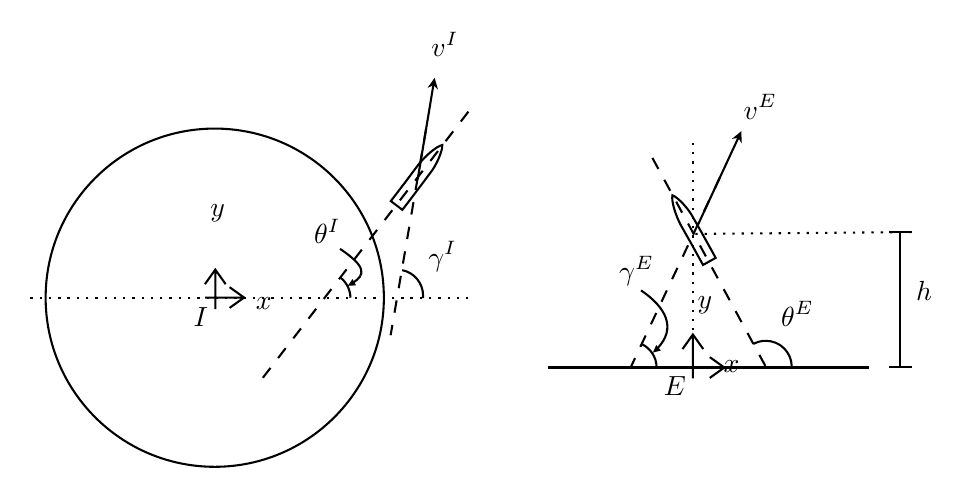
\begin{tikzpicture}[x=0.75pt,y=0.75pt,yscale=-1,xscale=1]
%uncomment if require: \path (0,300); %set diagram left start at 0, and has height of 300

%Shape: Circle [id:dp51055599617159] 
\draw   (13.15,136.59) .. controls (13.15,91.59) and (49.63,55.11) .. (94.63,55.11) .. controls (139.63,55.11) and (176.11,91.59) .. (176.11,136.59) .. controls (176.11,181.59) and (139.63,218.07) .. (94.63,218.07) .. controls (49.63,218.07) and (13.15,181.59) .. (13.15,136.59) -- cycle ;
%Shape: Polygon Curved [id:ds6809545569289366] 
\draw   (179.46,90.05) .. controls (188.94,77.65) and (184.18,83.93) .. (192.66,72.6) .. controls (195.98,68.34) and (201.51,63.56) .. (204.24,63.06) .. controls (204.49,65.63) and (201.56,72.74) .. (198.23,76.8) .. controls (192.12,84.99) and (188.87,89.29) .. (185.03,94.25) .. controls (182.08,92.03) and (181.97,91.94) .. (179.46,90.05) -- cycle ;
%Shape: Axis 2D [id:dp9626184003262446] 
\draw  (90,136.52) -- (108.78,136.52)(94.9,123.07) -- (94.9,142.07) (101.78,131.52) -- (108.78,136.52) -- (101.78,141.52) (89.9,130.07) -- (94.9,123.07) -- (99.9,130.07)  ;
%Straight Lines [id:da1924884864647387] 
\draw  [dash pattern={on 4.5pt off 4.5pt}]  (216.85,46.96) -- (115.22,178.52) ;
%Straight Lines [id:da37646115217489307] 
\draw  [dash pattern={on 0.84pt off 2.51pt}]  (216.85,136.59) -- (5,136.59) ;
%Straight Lines [id:da29558918810699253] 
\draw    (192.41,79.56) -- (200.06,33.63) ;
\draw [shift={(200.56,30.67)}, rotate = 459.46] [fill={rgb, 255:red, 0; green, 0; blue, 0 }  ][line width=0.08]  [draw opacity=0] (5.36,-2.57) -- (0,0) -- (5.36,2.57) -- (3.56,0) -- cycle    ;
%Straight Lines [id:da1751673672889571] 
\draw  [dash pattern={on 4.5pt off 4.5pt}]  (196.48,55.11) -- (179.37,154.68) ;
%Shape: Arc [id:dp12677215234005246] 
\draw  [draw opacity=0] (154.89,126.69) .. controls (157.95,128.93) and (159.95,132.54) .. (160,136.61) -- (147.5,136.77) -- cycle ; \draw   (154.89,126.69) .. controls (157.95,128.93) and (159.95,132.54) .. (160,136.61) ;
%Curve Lines [id:da5665026144335095] 
\draw    (155,113.07) .. controls (168.02,121.82) and (167.01,125.65) .. (161.3,129.35) ;
\draw [shift={(158.73,130.87)}, rotate = 331.11] [fill={rgb, 255:red, 0; green, 0; blue, 0 }  ][line width=0.08]  [draw opacity=0] (3.57,-1.72) -- (0,0) -- (3.57,1.72) -- cycle    ;
%Shape: Arc [id:dp5354114265871299] 
\draw  [draw opacity=0] (184.96,123.32) .. controls (190.69,124.46) and (195,129.51) .. (195,135.57) .. controls (195,135.98) and (194.98,136.38) .. (194.94,136.77) -- (182.5,135.57) -- cycle ; \draw   (184.96,123.32) .. controls (190.69,124.46) and (195,129.51) .. (195,135.57) .. controls (195,135.98) and (194.98,136.38) .. (194.94,136.77) ;
%Straight Lines [id:da09739935091747198] 
\draw    (255,170.24) -- (410,170.24) ;
%Shape: Polygon Curved [id:ds26667189428799865] 
\draw   (329.88,120.82) .. controls (322.34,107.15) and (326.18,114.03) .. (319.22,101.71) .. controls (316.65,96.96) and (314.51,89.97) .. (315.15,87.27) .. controls (317.6,88.08) and (322.93,93.62) .. (325.31,98.31) .. controls (330.34,107.19) and (332.97,111.91) .. (335.97,117.42) .. controls (332.74,119.22) and (332.62,119.29) .. (329.88,120.82) -- cycle ;
%Straight Lines [id:da7297056862448432] 
\draw  [dash pattern={on 4.5pt off 4.5pt}]  (305.49,69.25) -- (360.13,169.86) ;
%Shape: Arc [id:dp12318249729336173] 
\draw  [draw opacity=0] (354.11,158.9) .. controls (355.9,157.92) and (357.95,157.36) .. (360.13,157.36) .. controls (366.97,157.36) and (372.54,162.87) .. (372.62,169.7) -- (360.13,169.86) -- cycle ; \draw   (354.11,158.9) .. controls (355.9,157.92) and (357.95,157.36) .. (360.13,157.36) .. controls (366.97,157.36) and (372.54,162.87) .. (372.62,169.7) ;
%Straight Lines [id:da4987913292112276] 
\draw    (327.53,101.28) -- (347.12,59.03) ;
\draw [shift={(348.38,56.31)}, rotate = 474.87] [fill={rgb, 255:red, 0; green, 0; blue, 0 }  ][line width=0.08]  [draw opacity=0] (5.36,-2.57) -- (0,0) -- (5.36,2.57) -- (3.56,0) -- cycle    ;
%Straight Lines [id:da987115428584298] 
\draw  [dash pattern={on 4.5pt off 4.5pt}]  (337.95,78.8) -- (295,170.24) ;
%Shape: Arc [id:dp774819291660263] 
\draw  [draw opacity=0] (300.39,158.96) .. controls (304.55,160.95) and (307.44,165.17) .. (307.5,170.07) -- (295,170.24) -- cycle ; \draw   (300.39,158.96) .. controls (304.55,160.95) and (307.44,165.17) .. (307.5,170.07) ;
%Shape: Axis 2D [id:dp9530351851557042] 
\draw  (319.78,170.24) -- (340.15,170.24)(325,154.34) -- (325,175.45) (333.15,165.24) -- (340.15,170.24) -- (333.15,175.24) (320,161.34) -- (325,154.34) -- (330,161.34)  ;
%Straight Lines [id:da013198128788144192] 
\draw  [dash pattern={on 0.84pt off 2.51pt}]  (325,170.24) -- (325,151.52) -- (325,60.24) ;
%Curve Lines [id:da6766567652828324] 
\draw    (300,133.07) .. controls (311.91,141.12) and (317.43,151.22) .. (307.77,161.14) ;
\draw [shift={(305.73,163.04)}, rotate = 319.63] [fill={rgb, 255:red, 0; green, 0; blue, 0 }  ][line width=0.08]  [draw opacity=0] (3.57,-1.72) -- (0,0) -- (3.57,1.72) -- cycle    ;
%Straight Lines [id:da6854040010200555] 
\draw    (425,105) -- (425,170) ;
\draw [shift={(425,170)}, rotate = 270] [color={rgb, 255:red, 0; green, 0; blue, 0 }  ][line width=0.75]    (0,5.59) -- (0,-5.59)   ;
\draw [shift={(425,105)}, rotate = 270] [color={rgb, 255:red, 0; green, 0; blue, 0 }  ][line width=0.75]    (0,5.59) -- (0,-5.59)   ;
%Straight Lines [id:da9376071875237115] 
\draw  [dash pattern={on 0.84pt off 2.51pt}]  (430,105) -- (325,105.88) ;

% Text Node
\draw (113,135.07) node [anchor=north west][inner sep=0.75pt]   [align=left] {$\displaystyle x$};
% Text Node
\draw (91,90.07) node [anchor=north west][inner sep=0.75pt]   [align=left] {$\displaystyle y$};
% Text Node
\draw (83,140.07) node [anchor=north west][inner sep=0.75pt]   [align=left] {$\displaystyle I$};
% Text Node
\draw (197.5,7) node [anchor=north west][inner sep=0.75pt]   [align=left] {$\displaystyle v^{I}$};
% Text Node
\draw (141,97.07) node [anchor=north west][inner sep=0.75pt]   [align=left] {$\displaystyle \theta ^{I}$};
% Text Node
\draw (196,108.07) node [anchor=north west][inner sep=0.75pt]   [align=left] {$\displaystyle \gamma ^{I}$};
% Text Node
\draw (348,37.24) node [anchor=north west][inner sep=0.75pt]   [align=left] {$\displaystyle v^{E}$};
% Text Node
\draw (338.26,165.63) node [anchor=north west][inner sep=0.75pt]   [align=left] {$\displaystyle x$};
% Text Node
\draw (325.78,134.52) node [anchor=north west][inner sep=0.75pt]   [align=left] {$\displaystyle y$};
% Text Node
\draw (309.5,173.07) node [anchor=north west][inner sep=0.75pt]   [align=left] {$\displaystyle E$};
% Text Node
\draw (366,137) node [anchor=north west][inner sep=0.75pt]   [align=left] {$\displaystyle \theta ^{E}$};
% Text Node
\draw (288,115.07) node [anchor=north west][inner sep=0.75pt]   [align=left] {$\displaystyle \gamma ^{E}$};
% Text Node
\draw (431,127) node [anchor=north west][inner sep=0.75pt]   [align=left] {$\displaystyle h$};


\end{tikzpicture}
			
	\caption{Simulation reference frames and states.}
	\label{fig:to_refframes}
\end{figure}

